%% LyX 2.3.7 created this file.  For more info, see http://www.lyx.org/.
%% Do not edit unless you really know what you are doing.
\documentclass[oneside,english]{scrbook}
\usepackage[utf8]{inputenc}
\setcounter{secnumdepth}{3}
\setcounter{tocdepth}{1}
\synctex=-1
\usepackage{color}
\usepackage{babel}
\usepackage{float}
\usepackage{fancybox}
\usepackage{calc}
\usepackage{bm}
\usepackage{amsmath}
\usepackage{graphicx}
\usepackage{esint}
\usepackage[unicode=true,pdfusetitle,
 bookmarks=true,bookmarksnumbered=false,bookmarksopen=false,
 breaklinks=false,pdfborder={0 0 1},backref=section,colorlinks=false]
 {hyperref}

\makeatletter

%%%%%%%%%%%%%%%%%%%%%%%%%%%%%% LyX specific LaTeX commands.
\DeclareTextSymbolDefault{\textquotedbl}{T1}
%% Because html converters don't know tabularnewline
\providecommand{\tabularnewline}{\\}

%%%%%%%%%%%%%%%%%%%%%%%%%%%%%% Textclass specific LaTeX commands.
\newcommand{\lyxaddress}[1]{
	\par {\raggedright #1
	\vspace{1.4em}
	\noindent\par}
}

%%%%%%%%%%%%%%%%%%%%%%%%%%%%%% User specified LaTeX commands.
\usepackage{babel}
\usepackage{cite}




\usepackage{listings}
\renewcommand{\lstlistingname}{\inputencoding{latin9}Listing}

\makeatother

\usepackage{listings}
\renewcommand{\lstlistingname}{\inputencoding{latin9}Listing}

\begin{document}
\title{The Quantum and Stochastic Toolbox: xSPDE4}
\author{Peter D. Drummond}
\maketitle

\lyxaddress{\textbf{Centre for Quantum Science and Technology Theory, Swinburne
University of Technology, Melbourne, Victoria, Australia.}}

\newpage{} \tableofcontents{}\vspace{10pt}

\noindent \newpage{}

\chapter{Introduction}

\noindent \label{sec:Overview-of-xSPDE}

\textbf{\emph{xSPDE is an eXtensible Stochastic Partial Differential
Equation solver}}.

The xSPDE toolbox treats stochastic partial and ordinary differential
equations, with applications in biology, chemistry, engineering, medicine,
physics and quantum technologies. It computes statistical averages,
including time-step and/or sampling error estimation. xSPDE can provide
higher order convergence, Fourier spectra and probability densities.
The toolbox has graphical output and $\chi^{2}$ statistics, as well
as weighted, projected, or forward-backward equations. It can generate
input-output quantum spectra. All equations may have independent periodic,
Dirichlet, and Neumann or Robin boundary conditions in any dimension,
for any vector field component, and at either end of any interval.

xSPDE has functions that can numerically solve both ordinary and partial
differential stochastic equations of any type, obtaining correlations,
probabilities and averages. There are many equations of this type
\cite{Gardiner2009Stochastic,Drummond2014Quantum,Langevin1908theorie,Karatzas1991brownian,Glasserman2010monte}
in physics, chemistry, engineering, biology, medicine, and finance.
The toolbox has a core treating stochastic differential equations,
with averages, probability distributions and full error estimates.
There are stochastic extensions treating applications to partial differential
equations, projected equations, quantum stochastic equations, master
equations and quantum phase-space simulations.

Previous applications are in physics and quantum technology \cite{Opanchuk2013Quantum,Ng2019Phase,ramesh2022arcsine,peters2022limit,teh2017simulation,teh2018quantum,kiesewetter2022phase,teh2018creation,dechoum2016critical,drummond2017truncated,opanchuk2017one,drummond2017higher,ng2021fate,joseph2021hybrid,drummond2021time,drummond2020initial,ng2019nonlocal,busink2021stochastic,peters2021extremely,peters2022exceptional},
but the code has general applicability. The emphasis in xSPDE is on
combining a simple user interface with a wide range of useful functions,
including the essential features of averaging and global error estimates.
The code enables an efficient use memory and parallelism, which is
vital for large stochastic models, and it is able to be further extended
if needed.

The extensible structure of the code-base permits drop-in replacements
of the algorithms. Different simulations can be carried out sequentially.
This models different stages in an experiment or simulated environment.
It can be used with or without noise terms, and can use a range of
either built-in or user defined integration algorithms. This user
guide describes xSPDE4, which is an improved version of earlier toolboxes
\cite{Kiesewetter2016xSPDE,kiesewetter2023xspde3}.

xSPDE calculates and plots averages and probabilities of arbitrary
functions of any number of complex or real fields, as well as Fourier
transforms in time or space with any given dimensionality. Importantly,
it gives error estimates for both the discretization and sampling
error, but the algorithm, the step-size and the number of samples
used is up to the user to control to obtain the required error levels.

Ordinary and stochastic differential equations of many types can be
treated numerically \cite{Drummond1991Computer,Kloeden1992numerical},
including stochastic partial differential equations with space dependence
\cite{Werner1997Robust}. Comparative $\chi^{2}$ statistical tests
are available. Additional libraries exist for projected, forward-backward,
and weighted equations.

The algorithms included are designed to be useful and fast in many
practical applications. Higher order convergence is obtained through
order extrapolation. This allows higher-order convergence to be realized
in a uniform way. More complex higher-order algorithms are known \cite{Kloeden1992numerical,burrage2006comment},
which can be included if preferred, as the code is extensible.

The code can be used interactively or in batch mode. All graphs, data,
and input parameters, including default values, can be stored permanently
using standard file-types. It has a fully integrated graphics program,
xGRAPH. This is able to handle data of any dimensions, with multiple
types of graphical output, error-bars and comparisons.

xSPDE supports parallelism at both vector instruction and multiple
core level using array and parallel loop syntax. This version is Octave/Matlab
based. Matlab is a commercial product, GNU Octave \cite{eaton2012gnu}
is free and open-source. They each have excellent user interfaces
and reliable implementations. Full parallel operation currently requires
the Matlab parallel toolbox.

Chapters \ref{sec:SDE Theory} and \ref{sec:SPDE Theory} give background
information. Readers who are simply interested in how to use the code
can go directly to section \ref{sec:Simulating-an-SDE}.

Chapter \ref{sec:SDE Theory} has definitions and notations for stochastic
differential equations (SDEs). This is useful for understanding later
sections. The section includes Ito and Stratonovich calculus, probability
distributions and Fokker-Planck equations. It also explains and defines
the Fourier input-output spectra used in quantum technology.

Chapter \ref{sec:SPDE Theory} gives the concepts of stochastic partial
differential equations (SPDEs). It includes details of spectral methods
and the interaction picture approach. It has an explanation of how
Fourier transforms and discrete sine or cosine transforms are implemented.
It also explains how boundary conditions can be implemented using
finite differences.

Chapter \ref{sec:Simulating-an-SDE} describes the numerical solution
of SDEs with xSPDE. This includes an explanation of the user interface,
how to input parameters and equations, how to define the output in
terms of functional averages or probabilities, and how to define and
access auxiliary fields and noises. This chapter uses the default
algorithms, and a more detailed explanation is given in chapter \ref{sec:Algorithms}.

In Chapter \ref{sec:Simulating-an-SPDE}, the practical approach to
solving stochastic partial differential equations with xSPDE is explained.
The techniques used are an extension of the previous one, so a thorough
understanding of chapter \ref{sec:Simulating-an-SDE} is strongly
recommended.

Chapter \ref{sec:Algorithms} outlines the integration algorithms
used in the manual. It includes a number of extended integration libraries,
applicable to more specialized problems. This chapter also outlines
how integration errors, including time-step and stochastic errors,
can be estimated and displayed.

Chapter \ref{sec:xSIM-reference} provides a reference for the details
of the internals as well as a comprehensive explanation of the input
parameters useful in xSPDE simulations. This explains how to create
projects with separated computation and graphics, as well as workflow
and data storage. It also provides an extensive description of the
visualization aspects of xSPDE, using the integrated xGRAPH function,
which includes an automatic 'cascade' of graphic output where high
dimensional data is reduced to lower dimensional, visualizable data
through projections.

Input parameters related to this are described as well. Data can also
be graphed externally or stored for later analysis if preferred. Both
average and raw trajectory data can be stored. However, the storage
of raw data is generally not recommended, due to the large storage
requirements. Additional examples in Chapter \ref{sec:Examples} demonstrate
how to obtain parametric plots against input parameters. Plots of
one component value against another can be graphed. A function that
analyses convergence rates is also available.

Future implementations will include Julia versions, which are under
development and testing.

See:\emph{ }\textbf{www.github.com/peterddrummond/xspde\_matlab.}
For those familiar with earlier versions, a list of the main xSPDE
changes since the documentation of the previously published version
(v3.44){*}{*}{*}{*}{*}{*} \cite{Kiesewetter2016xSPDE} is as follows: 
\begin{enumerate}
\item Cell arrays for multiple variables with differing internal and space
dimensionality. 
\item Error-checking in space as well as time step-size
\item Phase-space simulations of quantum networks 
\item Quantum stochastic Schrödinger and master equations 
\item Jump algorithms as well as Gaussian noise methods 
\item Fast DST and DCT spectral methods for SPDEs with non-zero boundaries 
\end{enumerate}
\emph{xSPDE is distributed with no guarantee, under an open-source
license. Contributions and bug reports are welcome. }An alternative
approach to SPDEs \cite{Collecutt2001xmds,Dennis2013XMDS2} is available
in C++ at http://www.xmds.org/.

\newpage{}

\part{Fundamental Theory}

\chapter{SDE theory\label{sec:SDE Theory}}

\textbf{\emph{This chapter describes the basics of stochastic differential
equation (SDE) theory, in order to explain the background to the numerical
methods.}}

\section{General form}

A stochastic differential equation (SDE) is an equation with random
noise terms. These were introduced by Langevin to treat small particles
in fluids \cite{Langevin1908theorie}, and extended by Wiener, Ito
and Stratonovich \cite{wiener1930generalized,ito1996diffusion,stratonovich1960theory}.
The theory and its applications to biology, chemistry, engineering,
economics, physics, meteorology and other disciplines are treated
in many texts \cite{Karatzas1991brownian,VanKampen2007stochastic,Gardiner2009Stochastic,klebaner2012introduction,Drummond2014Quantum,Arnold1992stochastic}.

An ordinary stochastic differential equation in one time dimension
is,

\begin{equation}
\frac{\partial\mathbf{a}}{\partial t}=\mathbf{A}\left(\mathbf{a},t\right)+\underline{\mathbf{B}}\left(\mathbf{a},t\right)\cdot\mathbf{w}(t)\,.\label{eq:SDE}
\end{equation}
Here $\mathbf{a}$ is a real or complex vector, $\mathbf{A}$ is a
vector function, $\underline{\mathbf{B}}$ a matrix function and $\mathbf{w}$
is usually a delta-correlated real Gaussian noise vector such that:
\begin{eqnarray}
\left\langle w_{i}\left(t\right)w_{j}\left(t'\right)\right\rangle  & = & \delta\left(t-t'\right)\delta_{ij}.\label{eq:noise-correlations}
\end{eqnarray}

One can also have non-Gaussian noise or noise that is not delta-correlated.
Although these are somewhat less commonly treated, these alternatives
are often found in real applications.

\subsection{Observables}

In all cases, there are multiple independent trajectories, and one
is interested in probabilistic averages, where the unweighted average
of an observable $\mathbf{O}\left(\mathbf{a}\right)$, for $N_{s}$
trajectories $\mathbf{a}^{\left(n\right)}$ is: 
\begin{eqnarray}
\left\langle \mathbf{O}\right\rangle _{N_{s}} & = & \frac{1}{N_{s}}\sum_{n}\mathbf{O}\left(\mathbf{a}^{\left(n\right)}\right).\label{eq:averages-1}
\end{eqnarray}
In other types of stochastic equation \cite{graham1977path,Drummond2017forward},
there is a weight $\Omega\left(t\right)$ for each trajectory. This
has an additional equation of motion, where:

\begin{equation}
\frac{\partial\Omega}{\partial t}=A_{\Omega}\left(\mathbf{a},\Omega,t\right)+\underline{B}_{\Omega}\left(\mathbf{a},\Omega,t\right)\cdot\mathbf{w}(t)\,.\label{eq:SDE-2}
\end{equation}

The results for all mean values are then weighted by the term $\exp\left(\Omega\left(t\right)\right)$,
so that: 
\begin{equation}
\left\langle \mathbf{O}\right\rangle _{\Omega}=\frac{\sum_{n}\mathbf{O}\left(\mathbf{a}^{\left(n\right)}\right)\exp\left(\Omega^{\left(n\right)}\left(t\right)\right)}{\sum_{n}\exp\left(\Omega^{\left(n\right)}\left(t\right)\right)}.\label{eq:Weighted-averages-1}
\end{equation}
This expression reduces to the usual average if the weights are zero,
i.e, $\Omega=0$. Apart from the way that averages are treated, the
weight can simply be regarded as an additional term in the stochastic
differential equations. This simply means that one now has an equation
with an extra random field, so that $\mathbf{a}\rightarrow\left[\mathbf{a},\Omega\right]$,
together with a modified expression for the averages. This, in fact,
is how these equations are solved.

For reasons of efficiency, it is best to use ``breeding'' algorithms
to treat these numerically. This replicates highly weighted trajectories
with $\Omega^{\left(n\right)}\left(t\right)\gg0$ and removes trajectories
with $\Omega^{\left(n\right)}\ll0$, that have negligible weight.
The numerical method is described in section \ref{sec:Algorithms}.
The remainder of This chapter will focus on the most commonly treated
case of unweighted, Gaussian, delta-correlated noise.

\section{Stochastic calculus}

In the case of delta-correlated noise, the trajectories are not differentiable.
As a result, there are two main variants of stochastic calculus used
to define the derivatives, called Ito or Stratonovich \cite{Gardiner2009Stochastic,Arnold1992stochastic},
and xSPDE can be used for either type. The default algorithms are
designed for Stratonovich cases, since this is just ordinary calculus.
Ito calculus can be treated also, either using the directly applicable
Euler method, or else by appropriate transformations to a Stratonovich
form. One can also have a time-reversed or implicit Ito calculus \cite{Drummond1991Computer},
which is directly solved using an implicit Ito-Euler method.

A single step in time of duration $\Delta t$ uses finite noises $\mathbf{w}$
which are defined to be delta-correlated in the small time-step limit,
so that $\left\langle w_{i}w_{j}\right\rangle =\delta_{ij}/\Delta t.$

\subsection{Types of stochastic calculus}

The limits as $\Delta t\rightarrow0$ are taken differently for the
different types of stochastic calculus. Let $\mathbf{a}_{0}=\mathbf{a}\left(t_{0}\right)$,
$t_{1}=t_{0}+\Delta t$, $\mathbf{a}_{1}=\mathbf{a}\left(t_{1}\right)$,
$\bar{\mathbf{a}}=\left(\mathbf{a}_{1}+\mathbf{a}_{0}\right)/2$,
and $\bar{t}=t+\Delta t/2$, then the next step in time is: 
\begin{itemize}
\item Ito calculus - uses \textbf{initial-time} derivative evaluations 
\end{itemize}
\begin{equation}
\mathbf{a}_{1}=\mathbf{a}_{0}+\left[\mathbf{A}^{(I)}\left(\mathbf{a}_{0},t_{0}\right)+\underline{\mathbf{B}}\left(\mathbf{a}_{0},t_{0}\right)\cdot\mathbf{w}\right]\,\Delta t\,\,.\label{eq:SDE-1}
\end{equation}

\begin{itemize}
\item Stratonovich calculus - uses \textbf{midpoint} derivative evaluations 
\end{itemize}
\begin{equation}
\mathbf{a}_{1}=\mathbf{a}_{0}+\left[\mathbf{A}\left(\bar{\mathbf{a}},\bar{t}\right)+\underline{\mathbf{B}}\left(\bar{\mathbf{a}},\bar{t}\right)\cdot\mathbf{w}\right]\,\Delta t\,.\label{eq:SDE-1-1}
\end{equation}

\begin{itemize}
\item Implicit Ito calculus - uses \textbf{final-time} derivative evaluations 
\end{itemize}
\begin{equation}
\mathbf{a}_{1}=\mathbf{a}_{0}+\left[\mathbf{A}^{(I+)}\left(\mathbf{a}_{1},t_{1}\right)+\underline{\mathbf{B}}\left(\mathbf{a}_{1},t_{1}\right)\cdot\mathbf{w}\right]\,\Delta t\,\,.\label{eq:SDE-1-2}
\end{equation}
The drift term $\mathbf{A}$ is changed in Ito or implicit Ito calculus,
if the noise coefficient $B$ depends on the stochastic variable:
\begin{align}
A_{i}^{(I)} & =A_{i}+\frac{1}{2}B_{jk}\partial_{j}B_{ik},\label{eq:ItovsStratonovichDrift}\\
A_{i}^{(I+)} & =A_{i}-\frac{1}{2}B_{jk}\partial_{j}B_{ik}.
\end{align}

Here we define $\partial_{n}\equiv\partial/\partial a_{n}$ and we
use an Einstein convention of summing over all repeated indices.

\section{Interaction picture}

The interaction picture allows one to eliminate linear terms in the
time derivatives. It is especially useful for stochastic partial differential
equations, but it is applicable to stochastic equations as well. Suppose
there are linear terms $\underline{\mathbf{L}}$, so that $\mathbf{A}\left(\mathbf{a},t\right)=\mathbf{A}_{1}\left(\mathbf{a},t\right)+\underline{\mathbf{L}}\cdot\mathbf{a}\,$,
where $\underline{\mathbf{L}}$ is a constant matrix. The interaction
picture defines local variables $\tilde{\mathbf{a}}$ for the fields
$\mathbf{a}$.

It is convenient to introduce an abbreviated notation as: 
\begin{equation}
\begin{split}\begin{aligned}D\left(\mathbf{a}\right)=\mathbf{A}_{1}\left(\mathbf{a},t\right)+\underline{\mathbf{B}}\left(\mathbf{a},t\right)\cdot\mathbf{w}(t)\end{aligned}
\end{split}
,\label{eq:deriv_without_linear_term-1}
\end{equation}
so that one can write the differential equation as: 
\begin{equation}
\begin{split}\frac{\partial\mathbf{a}}{\partial t}=D\left(\mathbf{a}\right)+\underline{\mathbf{L}}\cdot\mathbf{a}.\end{split}
\end{equation}


\subsection{Linear propagator}

Next, we define a linear propagator. This is given formally by: 
\begin{equation}
\begin{split}\underline{\mathbf{P}}\left(\Delta t\right)=\exp\left(\Delta t\underline{\mathbf{L}}\right)\end{split}
.
\end{equation}
where $\Delta t=t-\bar{t}$, and $\bar{t}$ is the interaction picture
origin. Transforming the field $\mathbf{a}$ to an interaction picture
is achieved on defining: 
\begin{equation}
\tilde{\mathbf{a}}=\underline{\mathbf{P}}^{-1}\left(\Delta t\right)\mathbf{a}.
\end{equation}
As a result, the equation of motion is: 
\begin{equation}
\begin{split}\frac{\partial\tilde{\mathbf{a}}}{\partial t}=D\left(\underline{\mathbf{P}}\left(\Delta t\right)\tilde{\mathbf{a}}\right).\end{split}
\end{equation}

This removes linear terms, which can cause stiffness in the equations,
increasing the discretization error. Given the case of a completely
linear ODE or SDE, the trajectory solutions will be exact up to round-off
errors.

\section{Probability distributions}

Stochastic equations generate trajectories distributed with a probability
density $P\left(\mathbf{a}\right)$. These can be defined as an average
and hence can be evaluated stochastically, since: 
\begin{equation}
P\left(\mathbf{a}'\right)=\left\langle \delta\left(\mathbf{a}'-\mathbf{a}\right)\right\rangle .
\end{equation}
Here $\left\langle ..\right\rangle \equiv\left\langle ..\right\rangle _{\infty}$
is the infinite ensemble limit of the average over many trajectories.
The probability can be shown to follow a Fokker-Planck equation (FPE)
with positive semi-definite diffusion matrix, \cite{Risken1996,Gardiner2009Stochastic}:
\begin{equation}
\frac{\partial P}{\partial t}=\mathcal{L}P=\left[-\partial_{n}A_{n}^{(I)}+\frac{1}{2}\partial_{n}\partial_{m}B_{nk}B_{mk}\right]P\,,\label{eq:FPE}
\end{equation}
where the differential operators act on all terms to their right.

\subsection{Distribution averages}

The average of any observable $\mathbf{O}\left(\mathbf{a}\right)$
is obtained either by averaging over the stochastic trajectories numerically,
or by analytic calculations, using: 
\begin{eqnarray}
\left\langle \mathbf{O}\right\rangle  & = & \int\mathbf{O}\left(\mathbf{a}\right)P\left(\mathbf{a}\right)d\mathbf{a}.\label{eq:averages}
\end{eqnarray}

The dynamics of an observable or moment follows an adjoint equation,
where $\tilde{\mathcal{L}}$ is the adjoint of $\mathcal{L}$: 
\begin{equation}
\left\langle \frac{\partial\mathbf{O}}{\partial t}\right\rangle =\left\langle \tilde{\mathcal{L}}\mathbf{O}\right\rangle ,\label{eq:moment_equn}
\end{equation}
where: 
\begin{equation}
\left\langle \tilde{\mathcal{L}}\mathbf{O}\right\rangle =\left\langle \left[A_{n}^{(I)}\partial_{n}+\frac{1}{2}B_{nk}B_{mk}\partial_{n}\partial_{m}\right]\mathbf{O}\right\rangle .
\end{equation}
This equation allows the time-evolution of averages to be calculated
analytically in simple cases, given an initial distribution. However,
in more complex cases, a numerical simulation of the stochastic equations
is more practical, and this can be carried out with xSPDE or other
software.

\section{Example: random walk}

The first example of an SDE is the simplest possible stochastic equation
or Wiener process: 
\begin{equation}
\dot{a}=w(t)\,.\label{eq:Wiener_process}
\end{equation}

This has the solution that 
\begin{equation}
a\left(t\right)=a\left(0\right)+\int_{0}^{t}w\left(\tau\right)d\tau,
\end{equation}
which means that the initial mean value does not change in time: 
\begin{equation}
\left\langle a\left(t\right)\right\rangle =\left\langle a\left(0\right)\right\rangle .\label{eq:Wiener_mean}
\end{equation}


\subsection{Variance solution}

The noise correlation is non-vanishing from Eq \eqref{eq:noise-correlations},
so the variance must increase with time: 
\begin{align}
\left\langle a^{2}\left(t\right)\right\rangle  & =\left\langle a^{2}\left(0\right)\right\rangle +\int_{0}^{t}\int_{0}^{t}\left\langle w\left(\tau\right)w\left(\tau'\right)\right\rangle d\tau d\tau'\nonumber \\
 & =\left\langle a^{2}\left(0\right)\right\rangle +\int_{0}^{t}\int_{0}^{t}\delta\left(\tau-\tau'\right)d\tau d\tau'.
\end{align}

Integrating the delta function gives unity, which means that the second
moment and the variance both increase linearly with time:

\begin{align}
\left\langle a^{2}\left(t\right)\right\rangle  & =\left\langle a^{2}\left(0\right)\right\rangle +\int_{0}^{t}d\tau\nonumber \\
 & =\left\langle a^{2}\left(0\right)\right\rangle +t.\label{eq:Wiener_mean_square}
\end{align}

The probability follows an elementary diffusion equation: 
\begin{equation}
\frac{\partial P}{\partial t}=\frac{1}{2}\frac{\partial^{2}P}{\partial a^{2}}\,,\label{eq:FPE-1}
\end{equation}
which is an example of Eq \eqref{eq:FPE}. From this equation and
using Eq \eqref{eq:moment_equn}, the first two corresponding moment
equations in this case are 
\begin{align}
\frac{\partial}{\partial t}\left\langle a\right\rangle = & \left\langle \frac{1}{2}\frac{\partial^{2}}{\partial a^{2}}a\,\right\rangle =0\nonumber \\
\frac{\partial}{\partial t}\left\langle a^{2}\right\rangle = & \left\langle \frac{1}{2}\frac{\partial^{2}}{\partial a^{2}}a^{2}\,\right\rangle =1.
\end{align}

These differential equations are satisfied by the solutions obtained
directly from the stochastic equations, namely Eq \eqref{eq:Wiener_mean}
and Eq \eqref{eq:Wiener_mean_square}.

\section{Probability densities}

The Wiener process with an arbitrary noise strength has the stochastic
equation: 
\begin{equation}
\dot{a}=bw\left(t\right).
\end{equation}

The probability density satisfies the Fokker-Planck equation for diffusion,
\begin{equation}
\frac{\partial P}{\partial t}=\frac{b^{2}}{2}\frac{\partial^{2}}{\partial a^{2}}P\,.
\end{equation}

Then, if $x$ initially is Gaussian distributed, this has a Gaussian
distribution at time $t$ with: 
\begin{equation}
P\left(a\right)=\frac{1}{\sqrt{2\pi\sigma^{2}\left(t\right)}}\exp\left[-\frac{\left(a-\bar{a}\left(t\right)\right)^{2}}{2\sigma^{2}\left(t\right)}\right].
\end{equation}

Here: 
\begin{align}
\bar{a}\left(t\right) & =\bar{a}\left(0\right)\\
\sigma^{2}\left(t\right) & =\sigma^{2}\left(0\right)+b^{2}t.\nonumber 
\end{align}


\subsection{Distributions of functions}

Any function of the stochastic variables has a corresponding probability
density. For example, the distribution of $a^{2}$ has a $\chi^{2}$
distribution with a single degree of freedom, such that if $y=\left(a-\bar{a}\left(t\right)\right)^{2}/\sigma^{2}\left(t\right)$,
then:

\begin{equation}
P\left(y\right)=\frac{1}{\sqrt{2\pi y}}\exp\left[-\frac{y}{2}\right].
\end{equation}
Hence: 
\begin{equation}
P\left(a^{2}\right)=\frac{1}{\left|a-\bar{a}\left(t\right)\right|\sqrt{2\pi\sigma^{2}\left(t\right)}}\exp\left[-\frac{\left(a-\bar{a}\left(t\right)\right)^{2}}{2\sigma^{2}\left(t\right)}\right].
\end{equation}

More generally, it is often not known what the exact analytic solutions
are, and a numerical solution is employed. This can either use the
stochastic equation directly, or the Fokker-Planck equation, although
it is generally difficult to scale this to many variables or to partial
differential equations,

That is why we focus on the stochastic equation approach here, which
can be used to numerically calculate either the mean values or the
probability distributions in general cases.

\section{Fourier transforms}

Frequency spectra have many uses, especially for understanding the
steady-state fluctuations of any physical system in the presence of
noise, typically either thermal or quantum-mechanical, although the
noise could have other sources.

The time-domain spectral definition used here is: 
\begin{align}
\tilde{a}(\omega) & =\frac{1}{\sqrt{2\pi}}\int e^{i\omega t}a(t)dt\,\nonumber \\
a(t) & =\frac{1}{\sqrt{2\pi}}\int e^{-i\omega t}\tilde{a}(\omega)d\omega.\,
\end{align}

As a simple example, a sinusoidal oscillation in the form 
\begin{equation}
a(t)=\cos\left(\omega_{0}t\right).
\end{equation}
between $t=-T/2$ and $t=T/2$ has a Fourier transform given by: 
\begin{align}
\tilde{a}(\omega) & =\frac{1}{2\sqrt{2\pi}}\int_{-T/2}^{T/2}\left[e^{i\left(\omega-\omega_{0}\right)t}+e^{i\left(\omega+\omega_{0}\right)t}\right]dt\,\\
 & =\frac{T}{2\sqrt{2\pi}}\left[sinc\left(\left(\omega-\omega_{0}\right)\frac{T}{2}\right)+sinc\left(\left(\omega+\omega_{0}\right)\frac{T}{2}\right)\right].\nonumber 
\end{align}


\subsection{Discrete Fourier transforms}

While exact in this analytic case, the definition above is impractical
for numerical calculations. In taking measurements and doing simulations,
one has a discrete set of data-points. Assuming the samples are at
fixed intervals, the best one can do in practical cases is a discrete
Fourier transform, with samples $\bar{a}(\bar{t}_{j})$ that are defined
as integrals over each small interval $dt$:

Let $\bar{a}(\bar{t}_{j})$ be the average over a small time interval:
\begin{equation}
\bar{a}(\bar{t}_{j})=\int_{t_{j}}^{t_{j}+dt}a(t)dt\,,\label{eq:field-average}
\end{equation}
then to a good approximation as $dt\rightarrow0$, provided $\omega_{n}$
is not too large, 
\begin{align}
\tilde{a}(\omega_{n}) & =\frac{\Delta t}{\sqrt{2\pi}}\sum_{j=1}^{N}e^{i\omega_{n}\bar{t}_{j}}\bar{a}(\bar{t}_{j})\,\nonumber \\
\bar{a}(\bar{t}_{j}) & =\frac{\Delta\omega}{\sqrt{2\pi}}\sum_{n=1}^{N}e^{-i\omega_{n}\bar{t}_{j}}\tilde{a}(\omega_{n})\,.
\end{align}

These also form an invertible pair provided that $\Delta t\Delta\omega=2\pi/N$.
As well as being more practical, this is very efficient due to the
fast Cooley-Tukey (FFT) algorithm \cite{Cooley1965Algorithm}, allowing
computation on time-scales of $O\left(N\ln N\right)$ rather than
$O\left(N^{2}\right)$ as one might expect.

When taking Fourier transforms in the time-domain, xSPDE does a time-averaging
of all fields over the current time-step, using the available coarse
and fine time-samples. This is done by averaging the field before
and after the stochastic time-step. The methods used for this are
described in greater detail in Section (\ref{sec:Time-domain-spectra}).

\section{\label{sec:Quantum-phase-space-equations}Quantum phase-space}

One useful application of stochastic equations is in quantum technologies,
where stochastic methods are generally much more scalable than other
methods \cite{Opanchuk2019Mesoscopic,Opanchuk2019Robustness}. This
approach started when Schrödinger \cite{Schrodinger1926Constant}
pointed out that quantum oscillators can have classical equations.
Wigner, Moyal and Glauber extended this to other systems \cite{Wigner1932Quantum,Moyal1949Quantum,Glauber1963Coherent}.
In lasers and quantum optics \cite{Louisell1973Quantum,gardiner2004quantum,Carmichael2002Statistical,Drummond2014Quantum},
it is used to obtain SDEs for quantum systems coupled to reservoirs.

For the case of bosons, any $M$-mode quantum density matrix $\hat{\rho}$
may be written in a unified quantum phase-space form as: 
\begin{equation}
\hat{\rho}=\int d^{2M}\bm{\alpha}d^{2M}\bm{\beta}P_{\sigma}\left(\bm{\alpha},\bm{\beta}\right)\hat{\Lambda}_{\sigma}\left(\bm{\alpha},\bm{\beta}\right),
\end{equation}
where $P_{\sigma}$ is the $\sigma$-ordered phase-space distribution
function, and $\bm{\alpha}=\left[\alpha_{1},\ldots\alpha_{M}\right]$.
The basis, $\hat{\Lambda}_{\sigma}$, is a Gaussian function of annihilation
and creation operators (\cite{Corney2003Gaussian}), whose variance
depends on $\sigma$. This is defined as the variance of $\alpha\beta$
due to vacuum fluctuations, in the operator ordering of the representation.

For clarity, we hats like $\hat{a}$ are used here to indicate operators
that do not commute with each other, as opposed to stochastic variables
like $\alpha$ that do commute. For any given operator ordering, it
is always possible to find a probability distribution such that the
expectation of an operator product equals the stochastic variable
correlations \cite{Dirac1945Analogy}.

\subsection{Positive-P representation}

The above expansion leads to different statistics and noise terms
depending on the operator ordering. For example, in the normally ordered
positive P-representation where $\sigma=0$, the operator basis is
\begin{equation}
\hat{\Lambda}\left(\bm{\alpha},\bm{\beta}\right)\equiv\frac{\left|\bm{\alpha}\right\rangle \left\langle \bm{\beta}^{*}\right|}{\left\langle \bm{\beta}^{*}\right|\left.\bm{\alpha}\right\rangle }\,.
\end{equation}
Here $\bm{\beta}=\bm{\alpha}^{\dagger}\sim\hat{\bm{a}}^{\dagger}$
is a stochastic variable conjugate in the mean to $\bm{\alpha}^{*}$.
Any quantum state has a positive representation of this type \cite{Drummond1980Generalised},
and normally ordered coherence functions are moments of the distribution
with:

\begin{equation}
\left\langle \hat{a}_{m_{1}}^{\dagger}\ldots\hat{a}_{m_{n}}\right\rangle =\int d^{2M}\bm{\alpha}d^{2M}\bm{\beta}\left[\beta_{m_{1}}\ldots\alpha_{m_{n}}\right]P\left(\bm{\alpha},\bm{\beta}\right).\,\label{eq:nonclassical correlation}
\end{equation}

The Glauber-Sudarshan representation used in laser physics is obtained
for $\bm{\beta}=\bm{\alpha}^{*}$, so that the two variables are exactly
conjugate:

\begin{equation}
\hat{\rho}=\int d^{2M}\bm{\alpha}P\left(\bm{\alpha}\right)\left|\bm{\alpha}\right\rangle \left\langle \bm{\alpha}\right|.
\end{equation}
In this case, the total number of stochastic variables is halved,
but nonclassical squeezed or entangled states cannot be represented
as a positive distribution. Two additional frequently utilized representations
are the Wigner ($\sigma=1/2)$ and Husimi ($\sigma=1)$ representations,
characterized by symmetric ordering and anti-normal ordering, respectively.
These also have a classical phase-space with $\bm{\beta}=\bm{\alpha}^{*}$.

\subsection{Master equations}

The dynamics of a quantum system coupled to a reservoir is described
by a master equation. In the Markovian (high-frequency) limit, the
general quantum master equation for a dissipative quantum system with
damping rates $\Gamma_{j}$ is 
\begin{align}
{\frac{\partial\hat{\rho}}{\partial t}} & =\frac{1}{i\hbar}\left[\hat{H}_{sys},\hat{\rho}\right]+\sum_{j}\Gamma_{j}\left(\bar{n}_{j}+1\right)(2\hat{A}_{j}\hat{\rho}\hat{A}_{j}^{\dagger}-\hat{A}_{j}^{\dagger}\hat{A}_{j}\hat{\rho}-\hat{\rho}\hat{A}_{j}^{\dagger}\hat{A}_{j})\,\,\nonumber \\
 & +\sum_{j}\Gamma_{j}\bar{n}_{j}(2\hat{A}_{j}^{\dagger}\hat{\rho}\hat{A}_{j}-\hat{A}_{j}\hat{A}_{j}^{\dagger}\hat{\rho}-\hat{\rho}\hat{A}_{j}\hat{A}_{j}^{\dagger})\,\,,\label{eq:master-equation}
\end{align}
where $\Gamma_{j}$ is a damping rate for reservoir couplings to the
operator $\hat{A}_{j}$, $\bar{n}_{j}$ is the finite temperature
reservoir occupation, and the typical damping operators are:

\begin{table}
\begin{centering}
\begin{tabular}{|c|c|c|}
\hline 
Damping operator ($\hat{A}_{j}$)  & $\Gamma_{j}$  & Physical interpretation\tabularnewline
\hline 
$\hat{a}_{j}$  & $\gamma_{j}$  & Linear amplitude loss (units $s^{-1}$)\tabularnewline
\hline 
$\hat{a}_{j}^{\dagger}$  & $g_{j}$  & Linear amplitude gain (units $s^{-1}$)\tabularnewline
\hline 
$\hat{a}_{j}^{\dagger}\hat{a}_{j}$  & $\gamma_{j}^{p}$  & Phase decay rate gain (units $s^{-1}$)\tabularnewline
\hline 
$\hat{a}_{j}^{2}$  & $\kappa_{j}/2$  & nonlinear amplitude loss (units $s^{-1}$). \tabularnewline
\hline 
\end{tabular}
\par\end{centering}
\caption{Typical types of quantum damping term}
\end{table}

The operator equations are mapped to differential equations with the
equivalences:

\begin{eqnarray}
\hat{a}_{n}^{\dagger}\hat{\rho} & \rightarrow & \left[\beta_{n}+\left(\sigma-1\right)\frac{\partial}{\partial\alpha_{n}}\right]P_{\sigma}\nonumber \\
\hat{a}_{n}\hat{\rho} & \rightarrow & \left[\alpha_{n}+\sigma\frac{\partial}{\partial\beta_{n}}\right]P_{\sigma}\nonumber \\
\hat{\rho}\hat{a}_{n} & \rightarrow & \left[\alpha_{n}+\left(\sigma-1\right)\frac{\partial}{\partial\beta_{n}}\right]P_{\sigma}\nonumber \\
\hat{\rho}\hat{a}_{n}^{\dagger} & \rightarrow & \left[\beta_{n}+\sigma\frac{\partial}{\partial\alpha_{n}}\right]P_{\sigma}\,.\label{eq:drummond_identities-1-1}
\end{eqnarray}

The operator mappings give a differential equation. If it has a second-order
positive-definite form it is a Fokker-Planck equation equivalent to
an SDE, or an SPDE for quantum fields \cite{Carter1987Squeezing}.
The noise can be additive or multiplicative, depending on the problem.
Not all cases give stable FPE equations \cite{Deuar2002Gauge}, and
truncation is required for the Wigner representation if the Hamiltonian
is nonlinear \cite{Steel1998Dynamical}.

The total noise includes internal quantum noise generated from the
Hamiltonian term $\hat{H}_{sys}$, as well as reservoir noise terms
generated from the coupling to the reservoir operators, which is proportional
to $\Gamma_{j}$. There is a similar behavior in classical systems,
except that these correspond to a high-temperature limit, and in most
cases only have external reservoir noise from thermal fluctuations.

\section{Damped harmonic oscillator\label{sec:Damped-harmonic-oscillator}}

As an example, take the damped quantum harmonic oscillator. This has
the Hamiltonian $H=\omega_{0}\hat{a}^{\dagger}\hat{a}$. If damping
is added, it obeys the master equation 
\begin{align}
\frac{d\hat{\rho}}{dt} & =\frac{-i}{\hbar}[\omega_{0}\hat{a}^{\dagger}\hat{a},\rho]+\gamma\left(1+\bar{n}\right)(2\hat{a}\rho\hat{a}^{\dagger}-\hat{a}^{\dagger}\hat{a}\rho-\rho\hat{a}^{\dagger}\hat{a})\nonumber \\
 & +\gamma\bar{n}(2\hat{a}^{\dagger}\rho\hat{a}-\hat{a}\hat{a}^{\dagger}\rho-\rho\hat{a}\hat{a}^{\dagger}).
\end{align}
This leads to a random walk in a complex space \cite{Gardiner2009Stochastic,Drummond2014Quantum},
\begin{align}
\frac{d\alpha}{dt} & =-\left(\gamma+i\omega_{0}\right)\alpha+\sqrt{2\gamma\left(\sigma+\bar{n}\right)}\zeta(t)\nonumber \\
\frac{d\beta}{dt} & =-\left(\gamma-i\omega_{0}\right)\beta+\sqrt{2\gamma\left(\sigma+\bar{n}\right)}\zeta^{*}(t),
\end{align}
where the noise is complex and $\zeta(t)=\left(w_{1}(t)+iw_{2}(t)\right)/\sqrt{2}$.
The correlations are 
\begin{align}
\left\langle \zeta(t)\left(\zeta(t')\right)^{*}\right\rangle  & =\delta\left(t-t'\right)\nonumber \\
\left\langle \zeta(\omega)\left(\zeta\left(\omega'\right)\right)^{*}\right\rangle  & =\delta\left(\omega-\omega'\right).
\end{align}


\subsection{Wigner representation}

In the zero temperature Wigner case with $\gamma=$1, $\sigma=1/2$,
and in a rotating frame so that $\omega_{0}=0$, the probability follows
the Fokker-Planck equation: 
\begin{equation}
\frac{\partial P}{\partial t}=\left[\frac{\partial}{\partial\alpha_{x}}\alpha_{x}\,+\frac{\partial}{\partial\alpha_{y}}\alpha_{y}+\frac{1}{4}\left(\frac{\partial^{2}}{\partial\alpha_{x}^{2}}\,+\frac{\partial^{2}}{\partial\alpha_{y}^{2}}\right)\,\right]P\,,\label{eq:FPE-1-1}
\end{equation}
which is an example of Eq \eqref{eq:FPE}. Ignoring terms that vanish
or can be obtained from symmetry, the first corresponding moment equations
in each of the real and imaginary directions are 
\begin{align}
\frac{\partial}{\partial t}\left\langle \alpha_{x}\right\rangle = & \left\langle -\alpha_{x}\frac{\partial}{\partial\alpha_{x}}\alpha_{x}\,\right\rangle =-\left\langle \alpha_{x}\,\right\rangle \nonumber \\
\frac{\partial}{\partial t}\left\langle \alpha_{x}\alpha_{y}\right\rangle = & \left\langle -\left(\alpha_{x}\frac{\partial}{\partial\alpha_{x}}+\alpha_{y}\frac{\partial}{\partial\alpha_{y}}\,\right)\alpha_{x}\alpha_{y}\,\right\rangle =-\left\langle \alpha_{x}\alpha_{y}\,\right\rangle \nonumber \\
\frac{\partial}{\partial t}\left\langle \alpha_{x}^{2}\right\rangle = & \left\langle \left(-\alpha_{x}\frac{\partial}{\partial\alpha_{x}}+\frac{1}{4}\frac{\partial^{2}}{\partial\alpha_{x}^{2}}\,\right)\alpha_{x}^{2}\,\right\rangle =\frac{1}{2}-2\left\langle \alpha_{x}^{2}\,\right\rangle .
\end{align}

The steady-state is therefore a Gaussian distribution with $\left\langle \alpha_{x,y}\,\right\rangle =0$,
$\left\langle \alpha_{x}\alpha_{y}\,\right\rangle =0$ and $\left\langle \alpha_{x,y}^{2}\,\right\rangle =1/4$.
One can use an initial condition of $\alpha=(v_{1}+iv_{2})/2$, with
$\left\langle v_{i}^{2}\right\rangle =1/2$, in order to replicate
the steady state, which is a Gaussian with$\left\langle \alpha_{x}\,\right\rangle =\left\langle \alpha_{y}\,\right\rangle =0$
and$\left\langle \alpha_{x}^{2}\,\right\rangle =\left\langle \alpha_{y}^{2}\,\right\rangle =1/4$.

\subsection{Internal spectrum}

Neglecting any boundary terms, the equation in frequency space is:

\begin{equation}
-i\omega\tilde{\alpha}(\omega)=-\tilde{\alpha}(\omega)+\tilde{\zeta}(\omega).
\end{equation}

For sufficiently long times, the solution in frequency space - where
$\omega=2\pi f$ is the angular frequency - is therefore given by:
\begin{equation}
\tilde{\alpha}\left(\omega\right)=\frac{\tilde{\zeta}(\omega)}{1-i\omega}.
\end{equation}
The expectation value of the noise spectrum, $\left\langle \left|\tilde{\alpha}(\omega)\right|^{2}\right\rangle $
in the long time limit, is: 
\begin{eqnarray}
\left\langle \left|\tilde{\alpha}(\omega)\right|^{2}\right\rangle  & = & \frac{1}{2\pi\left(1+\omega^{2}\right)}\int\int e^{-i\omega(t-t')}\left\langle \zeta(t)\zeta^{*}(t')\right\rangle dtdt'\,.\nonumber \\
 & = & \frac{T}{2\pi\left(1+\omega^{2}\right)}.\label{eq:spectra_SHO}
\end{eqnarray}

This equation can also be used for some classical problems, which
correspond to the high-temperature limit of $\bar{n}\gg1$.

\section{Input-output spectra}

The spectrum of an internal field variable is not the one that is
usually measured. An important application of stochastic equations
is therefore in calculating output, measured spectra of lasers, quantum
optics, opto-mechanics and quantum circuits \cite{gardiner2004quantum,Kiesewetter2014Scalable}.
These have the feature that the measured output spectrum may also
include noise from reflected fields at the input/output ports. If
the quantum noise term in the Heisenberg equations for a cavity operator
$\hat{a}_{c}$ is given by: $\dot{\hat{a}}_{c}\sim..+\sqrt{2\gamma}\hat{a}_{in}(t),$
then the corresponding operator input-output relations are $\hat{a}_{out}(t)+\hat{a}_{in}(t)=\sqrt{2\gamma}\hat{a}_{c}$.

In quantum phase-space for the case of the harmonic oscillator or
similar systems, $\alpha_{in}=\sqrt{\sigma+\bar{n}}\zeta$ is the
noise term in the Langevin equation. The output fields $\alpha_{out}$
that are measured are given by: 
\begin{align}
\alpha_{out} & =\sqrt{2\gamma}\alpha-\alpha_{in}.
\end{align}

Hence one must include in the spectrum both the internal mode variables
and the noise terms themselves. Solving for the spectra, one obtains
auxiliary fields with 
\begin{align}
\tilde{\alpha}_{in}(\omega) & =\sqrt{\sigma+\bar{n}}\tilde{\zeta}(\omega)\\
\tilde{\alpha}_{out}(\omega) & =\sqrt{2\gamma}\tilde{a}(\omega)-\sqrt{\sigma+\bar{n}}\tilde{\zeta}(\omega).\nonumber 
\end{align}

In summary, it is the output fields that are amplified and measured.
Hence one must be able to compute the spectra of the output fields
for experimental comparisons. These have the additional feature that
they include the reservoir noise $\tilde{\zeta}(\omega)$, evaluated
at the same time as the field is evaluated, since the reservoir noise
is the input here. In xSPDE these are called \emph{auxfields}.

\subsection{Steady-state result}

Consider the example of Section (\ref{sec:Damped-harmonic-oscillator}),
in the Wigner representation case with $\gamma=1$, $\sigma=1/2$
and $\bar{n}=0$. Over long time-scales, so that one is in the steady
state, the solution for $\tilde{a}_{out}$ is that: 
\begin{align}
\tilde{\alpha}_{out}(\omega) & =\sqrt{2}\left[\frac{1}{1-i\omega}-\frac{1}{2}\right]\tilde{\zeta}(\omega)\nonumber \\
 & =\frac{1}{\sqrt{2}}\left[\frac{1+i\omega}{1-i\omega}\right]\tilde{\zeta}(\omega).
\end{align}

This gives the following expectation values: 
\begin{align}
\left\langle \tilde{\alpha}_{out}(\omega)\left(\tilde{\alpha}_{out}(\omega)\left(\omega'\right)\right)^{*}\right\rangle  & =\frac{1}{2}\delta\left(\omega-\omega'\right)\nonumber \\
\left\langle \tilde{\alpha}_{in}(\omega)\left(\tilde{\alpha}_{in}(\omega)\left(\omega'\right)\right)^{*}\right\rangle  & =\frac{1}{2}\delta\left(\omega-\omega'\right).
\end{align}
These are the expectation values of the zero temperature quantum fluctuations
in the input and output channels. This means that the harmonic oscillator
in its ground state is in equilibrium with an external vacuum field
reservoir, also in its ground state. However, from Eq \eqref{eq:spectra_SHO},
the internal spectral correlations of the harmonic oscillator are
modified by the coupling.

While this is a simple result, exactly the same general type of behavior
occurs in more sophisticated cases. These may include many coupled
modes with nonlinearities. Additional or auxiliary fields that depend
both on noise terms and internal stochastic variables are required.
The soluble case given above is a useful test case, and it is treated
numerically later in the manual.

\section{Forward-backward stochastic equations}

General forward-backward (FB) equations have the following structure,
written as an integral equation to make it clear what the relevant
boundary conditions are:

\begin{align}
\mathbf{p}\left(t\right) & =\mathbf{p}\left(0,\mathbf{q}\left(0\right)\right)+\int_{0}^{t}\left\{ \mathbf{A}^{p}\left[\mathbf{a}\left(t'\right)\right]dt'+\underline{\mathbf{B}}^{p}\left[\mathbf{a}\left(t'\right)\right]\cdot d\mathbf{w}^{p}(t')\right\} \nonumber \\
\mathbf{q}\left(t\right) & =\mathbf{q}\left(T\right)+\int_{t}^{T}\left\{ \mathbf{A}^{q}\left[\mathbf{a}\left(t'\right)\right]dt'+\underline{\mathbf{B}}^{q}\left[\mathbf{a}\left(t'\right)\right]\cdot d\mathbf{w}^{q}(t')\right\} .
\end{align}
Here, $\mathbf{a}=\left[\mathbf{p},\mathbf{q}\right]$ includes forward
components $\mathbf{p}$ and backwards components $\mathbf{q}$. These
have ``initial'' conditions in the past and the future, respectively,
and can depend on random inputs, just as with ordinary stochastic
equations. The equations are interpreted as having Stratonovich type
or symmetric limits to any products.

The noise terms $\mathbf{w}=\left[\mathbf{w}^{p},\mathbf{w}^{q}\right]$
are uncorrelated real Gaussian noises: 
\begin{equation}
\left\langle dw_{i}^{\alpha}\left(\mathbf{x}\right)dw_{j}^{\beta}\left(\mathbf{x}'\right)\right\rangle =\delta_{ij}\delta_{\alpha\beta}dt.
\end{equation}
This can also be written in differential form, where $t_{-}=T-t$,
as: 
\begin{align}
\frac{\partial\mathbf{p}}{\partial t} & =\mathbf{A}^{p}\left[\mathbf{a}\right]+\underline{\mathbf{B}}^{p}\left[\mathbf{a}\right]\cdot\mathbf{w}^{p}(t)\,\nonumber \\
\frac{\partial\mathbf{q}}{\partial t_{-}} & =\mathbf{A}^{q}\left[\mathbf{a}\right]+\underline{\mathbf{B}}^{q}\left[\mathbf{a}\right]\cdot\mathbf{w}^{q}(t)\,.
\end{align}

Other types of FB equations can be found in the mathematics literature,
as well as more sophisticated methods of solution.

\newpage{}

\chapter{Quantum theory\label{sec:Quantum Theory}}

\textbf{\emph{This chapter describes the quantum theory used in xSPDE,
to explain the background to the quantum methods.}}

\section{Master Equation}

The density matrix master equation is basic to quantum theory. It
has a memory requirement that scales as $e^{2\lambda M}$ for $M$
modes, where $\lambda=\ln(N_{max})$, and $N_{max}$ is the dimension
of the Hilbert space of a single mode. This becomes exponentially
difficult to solve numerically as $M\rightarrow\infty$.

The master equation treated here and elsewhere is repeated for reference
purposes. It has the standard Lindblad form that: 
\begin{align}
\dot{\rho} & =\mathcal{L}\rho\label{eq:Lindblad_Master_Equation}\\
 & =-i\left[\hat{H},\rho\right]+\sum_{j}\gamma_{j}\left(2\hat{L}_{j}\rho\hat{L}_{j}^{\dagger}-\hat{L}_{j}^{\dagger}\hat{L}_{j}\rho-\rho\hat{L}_{j}^{\dagger}\hat{L}_{j}\right)
\end{align}
Here, $H$ is the reversible system Hamiltonian, $L_{j}$ are operators
that couple the quantum system to the dissipative reservoir, and $\gamma_{j}$
is the decay rate.

Provide that $\rho$ is normalized, the expectation values of observables
$\hat{O}$ are given by: 
\begin{equation}
\left\langle \hat{O}\right\rangle =Tr\left(\rho\hat{O}\right)
\end{equation}
The definitions used here mean that for the case of linear damping
with $\hat{L}=\hat{a}$, the rate $\gamma$ is the amplitude decay
rate. This abstract notation does not include the effects of finite
temperatures, which are explained below.

The rate is written explicitly here. This is useful for xSPDE inputs,
which use standard dimensionless operators. Some references combine
the rate with the operator \cite{gisin1992quantum}, which implies
$\gamma=1.$ Others use a rate constant of $\kappa=2\gamma$, i.e.,
the number decay rate. Some combine \emph{this} rate with the operator,
defining $\hat{c}_{j}=\sqrt{2\gamma_{j}}\hat{L}_{j}$., giving a fourth
type of damping operator convention.

Including finite temperature reservoir occupation numbers $\bar{n}_{j}$
explicitly, the quantum master equation with damping rates $\Gamma_{j}$
is 
\begin{align}
{\frac{\partial\hat{\rho}}{\partial t}} & =-i\left[\hat{H},\hat{\rho}\right]+\sum_{j}\Gamma_{j}\left(\bar{n}_{j}+1\right)(2\hat{A}_{j}\hat{\rho}\hat{A}_{j}^{\dagger}-\hat{A}_{j}^{\dagger}\hat{A}_{j}\hat{\rho}-\hat{\rho}\hat{A}_{j}^{\dagger}\hat{A}_{j})\,\,\nonumber \\
 & +\sum_{j}\Gamma_{j}\bar{n}_{j}(2\hat{A}_{j}^{\dagger}\hat{\rho}\hat{A}_{j}-\hat{A}_{j}\hat{A}_{j}^{\dagger}\hat{\rho}-\hat{\rho}\hat{A}_{j}\hat{A}_{j}^{\dagger})\,\,,\label{eq:master-equation-1}
\end{align}
where $\Gamma_{j}$ is a zero temperature damping rate for reservoir
couplings to the operator $\hat{A}_{j}$, $\bar{n}_{j}$ is the finite
temperature reservoir occupation, and the typical damping operators
are:

\begin{table}
\begin{centering}
\begin{tabular}{|c|c|c|}
\hline 
Damping operator ($\hat{A}_{j}$)  & $\Gamma_{j}$  & Physical interpretation\tabularnewline
\hline 
$\hat{a}_{j}$  & $\gamma_{j}$  & Linear amplitude loss (units $s^{-1}$)\tabularnewline
\hline 
$\hat{a}_{j}^{\dagger}$  & $g_{j}$  & Linear amplitude gain (units $s^{-1}$)\tabularnewline
\hline 
$\hat{a}_{j}^{\dagger}\hat{a}_{j}$  & $\gamma_{j}^{p}$  & Phase decay rate gain (units $s^{-1}$)\tabularnewline
\hline 
$\hat{a}_{j}^{2}$  & $\kappa_{j}/2$  & nonlinear amplitude loss (units $s^{-1}$).\tabularnewline
\hline 
\end{tabular}
\par\end{centering}
\caption{Typical types of quantum damping term}
\end{table}


\section{Stochastic Schrödinger equation}

A stochastic Schrödinger equation (SSE) is an equation with noise
terms used to solve a dissipative master equation by random sampling,
and was originally developed for applications in quantum foundations
\cite{pearle1979toward,Ghirardi1986PhysRevD.34.470,gisin1992quantum}.
It has the advantage over a master equation that for large numbers
of modes it uses less storage. This requires $e^{\lambda M}$complex
numbers for the storage of an $M-$mode quantum system, compared to
$\sim e^{2\lambda M}$ for the master equation, where $\lambda=\log_{e}(N)$
for an $N$-level local Hilbert space. This is exponentially large,
but the memory required is less than with a density matrix equation,
doubling the number of modes that are accessible. The drawback is
that many parallel trajectories must be averaged in order to give
a low final sampling error.

An SSE can also be regarded in certain cases as providing a direct
simulation of the measurement process, which means that the information
recorded in a simulation is similar to the information measured in
a quantum experiment. This requires a suitable choice of the method,
sometimes called an ``unraveling'' and the stochastic integration
algorithm. Different unravellings mean different measurements and
different convergence rates.

There are many versions of the SSE, which use different normalization,
different random noises or different types of stochastic calculus.
Noises can be real or complex, and either continuous or with discrete
jumps. These are different ``unravellings'', and correspond physically
to distinct measurement devices and outcomes. They also have different
sampling errors.

Compared to phase-space expansions, the SSE method has the problem
that storage requirements are exponential in the system size, although
it may have lower sampling errors for high nonlinearities. This limits
mode numbers to $10-50$, depending on the size of the Hilbert space
per mode and the computational resources. The approach is most useful
for small mode numbers, especially for large nonlinearities.

\subsection{Normalized Ito SSE}

A widely used form of the continuous noise, normalized SSE is as follows
\cite{gisin1992quantum}, in the Ito calculus:

\begin{align}
d\left|\Psi\right\rangle  & =\left\{ -i\hat{H}+\sum_{j}\gamma_{j}\left(2\left\langle \hat{L}_{j}^{\dagger}\right\rangle _{\Psi}\hat{L}_{j}-\left\langle \hat{L}_{j}^{\dagger}\right\rangle _{\Psi}\left\langle \hat{L}_{j}\right\rangle _{\Psi}-\hat{L}_{j}^{\dagger}\hat{L}_{j}\right)\right\} \left|\Psi\right\rangle dt\nonumber \\
 & +\sum_{j}\sqrt{2\gamma_{j}}\Delta\hat{L}_{j}\left|\Psi\right\rangle d\xi_{j}.\label{eq:nonlinear SSE-1-2}
\end{align}
where $\Delta\hat{L}_{j}=\hat{L}_{j}-\left\langle \hat{L}_{j}\right\rangle _{\Psi}$,
and 
\begin{align}
\left\langle d\xi_{j}^{*}d\xi_{k}\right\rangle  & =\delta_{jk}dt.\nonumber \\
\left\langle d\xi_{j}d\xi_{k}\right\rangle  & =0.\label{eq:Complex noise}
\end{align}

A more general form of the normalized SSE \cite{rigo1997continuous}
in the Ito calculus is:

\begin{align}
d\left|\Psi\right\rangle  & =\left\{ -i\hat{H}+\sum_{j}\gamma_{j}\left(2\left\langle \hat{L}_{j}^{\dagger}\right\rangle _{\Psi}\hat{L}_{j}-\left\langle \hat{L}_{j}^{\dagger}\right\rangle _{\Psi}\left\langle \hat{L}_{j}\right\rangle _{\Psi}-\hat{L}_{j}^{\dagger}\hat{L}_{j}\right)\right\} \left|\Psi\right\rangle dt\nonumber \\
 & +\sum_{jn}\sqrt{2\gamma_{j}}\Delta\hat{L}_{j}\left|\Psi\right\rangle \alpha_{jn}d\zeta_{jn}.\label{eq:nonlinear SSE-1}
\end{align}
where we require that $\sum_{n}\left|\alpha_{jn}\right|^{2}=1$, and
\begin{align}
\left\langle d\zeta_{jn}\left(t\right)d\zeta_{km}\left(t'\right)\right\rangle  & =\delta_{jk}\delta_{nm}dt.
\end{align}

One can also include a unitary transformation, which we set to a delta
function for simplicity. When there is one noise per decay channel,
then $\alpha_{j}\left(t\right)=e^{i\phi_{j}}$, where $\phi_{j}$
is arbitrary. If there are two noises, then one can choose $\alpha_{j1}\left(t\right)=1/\sqrt{2}$,
and $\alpha_{j2}\left(t\right)=i/\sqrt{2}$., giving a complex noise
SDE, with $\xi_{j}=\left(\zeta_{1}+i\zeta_{2}\right)/\sqrt{2}$, as
above.

This can be written for $\left|\Psi\right\rangle \rightarrow\Psi_{\nu}$,
and $d\zeta_{jn}\rightarrow dw_{\sigma}$, as: 
\[
d\psi_{\mu}=A_{\mu}dt+B_{\mu\sigma}dw_{\sigma}
\]


\section{Stratonovich Equations}

To obtain standard calculus, one must transform to the Stratonovich
equation. This form of stochastic calculus allows integration algorithms
that often give lower errors \cite{Drummond1991Computer}. There are
also higher order methods for Ito equations, but these have greatly
increased complexity. Here we derive the Stratonovich correction \cite{stratonovich1960theory,Gardiner2009Stochastic},
which is obtained with $\hat{L}_{j}\left|\Psi\right\rangle \rightarrow L_{j\mu\nu}\Psi_{\nu}$
so that $\left\langle \hat{L}_{j}^{\dagger}\right\rangle _{\Psi}=\sum_{\sigma\rho}\Psi_{\sigma}^{*}L_{j\rho\sigma}^{*}\Psi_{\rho}$.

For complex noise as in Eq (\ref{eq:Complex noise}), the Stratonovich
drift is given by:

\begin{equation}
A_{\mu}=A_{\mu}^{(I)}-\frac{1}{2}\sum_{j\nu}B_{\nu j}^{*}\partial_{\nu}^{*}B_{\mu j}.
\end{equation}
On taking matrix elements in an orthogonal basis, and defining: 
\begin{equation}
\Delta L_{j\mu\nu}=L_{j\mu\nu}-\delta_{\mu\nu}\sum_{\sigma\rho}\Psi_{\rho}^{*}L_{j\rho\sigma}\Psi_{\sigma},
\end{equation}
one has:

\begin{align}
B_{\mu j} & =\sqrt{2\gamma_{j}}\Delta L_{j\mu\beta}\Psi_{\beta}\\
B_{\mu j}^{*} & =\sqrt{2\gamma_{j}}\Psi_{\beta}^{*}\Delta L_{j\mu\beta}^{*}.\nonumber 
\end{align}
On differentiating one therefore obtains: 
\begin{align}
\partial_{\nu}^{*}B_{\mu j} & =\sqrt{2\gamma_{j}}\sum_{\beta}\left[-\Psi_{\beta}\partial_{\nu}^{*}\left(\delta_{\mu\beta}\sum_{\sigma\rho}\Psi_{\rho}^{*}L_{j\rho\sigma}\Psi_{\sigma}\right)\right]\nonumber \\
 & =\sqrt{2\gamma_{j}}\left[-\Psi_{\mu}\sum_{\sigma}L_{j\nu\sigma}\Psi_{\sigma}\right].
\end{align}
The Stratonovich correction is given by: 
\begin{align}
-\frac{1}{2}\sum_{\nu,j}B_{\nu j}^{*}\partial_{\nu}^{*}B_{\mu j} & =-\sum_{j}\gamma_{j}\sum_{\nu,\alpha}\Psi_{\alpha}^{*}\Delta L_{j\nu\alpha}^{*}\left[-\Psi_{\mu}\sum_{\sigma}L_{j\nu\sigma}\Psi_{\sigma}\right]\nonumber \\
 & =\sum_{j}\gamma_{j}\left[\sum_{\nu\sigma\alpha}\Psi_{\alpha}^{*}\left(L_{j\nu\alpha}^{*}-\delta_{\nu\alpha}\left\langle \hat{L}_{j}^{\dagger}\right\rangle _{\Psi}\right)L_{j\nu\sigma}\Psi_{\sigma}\right]\Psi_{\mu}\nonumber \\
 & =\sum_{j}\gamma_{j}\left[\left\langle \hat{L}_{j}^{\dagger}\hat{L}_{j}\right\rangle _{\Psi}-\left\langle \hat{L}_{j}^{\dagger}\right\rangle _{\Psi}\left\langle \hat{L}_{j}\right\rangle _{\Psi}\right]\Psi_{\mu}.
\end{align}

In summary, the complex Ito SSE can be transformed to a nonlinear
Stratonovich stochastic differential equation which locally preserves
normalization for zero step-size \cite{Diosi1998PhysRevA.58.1699}.
This is called the quantum state diffusion model:

\begin{align}
\frac{d\left|\Psi\right\rangle }{dt} & =\left(-i\hat{H}-\sum_{j}\gamma_{j}\Delta\left[\hat{L}_{j}^{\dagger}\hat{L}_{j}\right]\right)\left|\Psi\right\rangle \nonumber \\
 & +\sum_{j}\left(2\gamma_{j}\left\langle \hat{L}_{j}^{\dagger}\right\rangle _{\Psi}+\sqrt{2\gamma_{j}}\xi_{j}\right)\Delta\hat{L}_{j}\left|\Psi\right\rangle \label{eq:nonlinear SSE}
\end{align}
where: 
\begin{equation}
\left\langle \xi_{j}\left(t\right)\xi_{j}^{*}\left(t'\right)\right\rangle =\delta_{kj}\delta\left(t-t'\right).
\end{equation}

Here, $\Delta\hat{L}_{j}\equiv\hat{L}_{j}-\left\langle \hat{L}_{j}\right\rangle _{\Psi}$
and the equation uses Stratonovich calculus. This preserves the norm
of the wave-function. Suppose the Stratonovich form has a dissipative
term $\Delta\hat{\mathcal{L}}_{s}$, where

\begin{equation}
\frac{d\left|\Psi\right\rangle }{dt}=\left\{ \Delta\hat{\mathcal{L}}_{s}-i\hat{H}\right\} \left|\Psi\right\rangle 
\end{equation}
Since it is a Stratonovich equation, one can use ordinary calculus
rules. Only dissipative terms can change the norm, and:

\begin{align}
\frac{d}{dt}\left\langle \Psi\right.\left|\Psi\right\rangle  & =\left\langle \Delta\left(\hat{\mathcal{L}}_{s}+\hat{\mathcal{L}}_{s}^{\dagger}\right)\right\rangle _{\psi}\nonumber \\
 & =\left\langle \hat{\mathcal{L}}_{s}+\hat{\mathcal{L}}_{s}^{\dagger}\right\rangle _{\psi}-\left\langle \hat{\mathcal{L}}_{s}+\hat{\mathcal{L}}_{s}^{\dagger}\right\rangle _{\psi}=0
\end{align}

For Ito equations, the trajectories have a norm error that grows with
time. While there are projective methods to prevent this, the result
has higher step-size errors \cite{Joseph2023midpoint}.To obtain observables,
one must use the ``double'' expectation indicating a quantum and
stochastic mean, where the wave-functions $\left|\Psi\right\rangle $
are normalized, and have all the same weight: 
\begin{equation}
\left\langle O\right\rangle \equiv\left\langle \left\langle \Psi\right|O\left|\Psi\right\rangle \right\rangle _{\xi}.
\end{equation}

Integrating this equation is best carried out with a projection at
each time-step to prevent the normalization changing, as derived elsewhere
\cite{Joseph2023midpoint}. This is implemented automatically within
xSPDE.

\subsection{Real noise Stratonovich equation}

For the real noise case, the correction term is: 
\begin{equation}
A_{\mu}=A_{\mu}^{(I)}-\frac{1}{2}\sum_{\sigma\nu}\left(B_{\nu\sigma}\partial_{\nu}+B_{\nu\sigma}^{*}\partial_{\nu}^{*}\right)B_{\mu\sigma},
\end{equation}
where $B_{\mu j}=\sqrt{2\gamma_{j}}\Delta L_{j\mu\beta}\Psi_{\beta}$.
Taking $n=1$ and $j=\sigma,$ the conjugate correction is given above
and is independent of $\alpha_{j}$. The first term is obtained from
differentiation of the noise matrix:

\begin{equation}
B_{\mu j}=\alpha_{j}\sqrt{2\gamma_{j}}\Delta L_{j\mu\beta}\Psi_{\beta}.
\end{equation}
hence one obtains that: 
\begin{align}
\partial_{\nu}B_{\mu j} & =\sqrt{2\gamma_{j}}\alpha_{j}\left[\Delta L_{j\mu\nu}-\sum_{\beta}\delta_{\mu\beta}\left[\Psi_{\rho}^{*}L_{j\rho\nu}\right]\Psi_{\beta}\right].
\end{align}
The additional correction is as follows: 
\begin{align}
-\frac{1}{2}\sum_{\nu j}B_{\nu j}\partial_{\nu}B_{\mu j} & =-\sum_{\nu j}\gamma_{j}\alpha_{j}^{2}\left[\Delta L_{j\mu\nu}-\Psi_{\rho}^{*}L_{j\rho\nu}\Psi_{\mu}\right]\Delta L_{j\nu\sigma}\Psi_{\sigma}\nonumber \\
 & =-\sum_{\nu j}\gamma_{j}\alpha_{j}^{2}\left(\Delta L_{j\mu\nu}\Delta L_{j\nu\sigma}\Psi_{\sigma}-\left[\Psi_{\rho}^{*}L_{j\rho\nu}\Delta L_{j\nu\sigma}\Psi_{\sigma}\right]\Psi_{\mu}\right).
\end{align}

Written in operator/wave-function terminology, the real correction
$\left|\delta A^{r}\right\rangle $is 
\begin{align}
\left|\delta A^{r}\right\rangle  & =-\sum_{\nu j}\gamma_{j}\alpha_{j}^{2}\left(\left[\Delta\hat{L}_{j}\Delta\hat{L}_{j}\right]-\left\langle \hat{L}_{j}\Delta\hat{L}_{j}\right\rangle _{\Psi}\right)\left|\Psi\right\rangle \nonumber \\
 & =-\sum_{\nu j}\gamma_{j}\alpha_{j}^{2}\left(\left[\hat{L}_{j}^{2}-2\hat{L}_{j}\left\langle \hat{L}_{j}\right\rangle _{\Psi}+\left\langle \hat{L}_{j}\right\rangle _{\Psi}^{2}\right]-\left\langle \hat{L}_{j}^{2}\right\rangle _{\Psi}+\left\langle \hat{L}_{j}\right\rangle _{\Psi}^{2}\right)\left|\Psi\right\rangle \nonumber \\
 & =\sum_{\nu j}\gamma_{j}\left(2\Delta\hat{L}_{j}\left\langle \alpha_{j}^{2}\hat{L}_{j}\right\rangle _{\Psi}-\Delta\left[\alpha_{j}^{2}\hat{L}_{j}^{2}\right]\right)\left|\Psi\right\rangle .
\end{align}
Combining both terms, and defining $\hat{X}_{j}=\hat{L}_{j}^{\dagger}+\alpha_{j}^{2}\hat{L}_{j}$,
one obtains a result known in the literature (Gambetta) for the case
$\alpha=1$; 
\begin{align}
\frac{d\left|\Psi\right\rangle }{dt} & =\left\{ -iH+\sum_{j}\gamma_{j}\left(2\left\langle \hat{X}_{j}\right\rangle _{\Psi}\Delta\hat{L}_{j}-\Delta\left[\hat{X}_{j}\hat{L}_{j}\right]\right)\right\} \left|\Psi\right\rangle \nonumber \\
 & +\sum_{j}\sqrt{2\gamma_{j}}\Delta\hat{L}_{j}\left|\Psi\right\rangle \alpha_{j}\zeta_{j}\left(t\right)
\end{align}

As with the complex noise case, this is explicitly norm-preserving
since the dissipative terms have zero quantum mean values for every
noise realization. This generic result reduces to the complex case
if one sets$\hat{X}_{j}=\hat{L}_{j}^{\dagger}$ and $\alpha_{j}\zeta_{j}\rightarrow\xi_{j}$.

\subsection{Stochastic master equation}

Although it provides no memory use improvements, there is a density
matrix version of this equation. It is derivable simply using the
product rule, since the above equation is in the Stratonovich calculus.
It is useful when simulating measurements when only some measurements
are being monitored, or if there is a measurement efficiency $\eta$:
\begin{align}
\frac{d\rho}{dt} & =\left(\frac{d}{dt}\left|\Psi\right\rangle \right)\left\langle \Psi\right|+\left|\Psi\right\rangle \left(\frac{d}{dt}\left\langle \Psi\right|\right)\nonumber \\
 & =-i\left[\hat{H},\rho\right]-\sum_{j}\left(\gamma_{j}\left[\Delta\left(\hat{L}_{j}^{\dagger}\hat{L}_{j}\right)\rho+h.c\right]\right)\\
 & +\sum_{j}\left[\left(2\gamma_{j}\left\langle \hat{L}_{j}^{\dagger}\right\rangle _{\Psi}+\sqrt{2\gamma_{j}}\xi_{j}\right)\Delta\hat{L}_{j}\rho+h.c\right]\label{eq:nonlinear SSE-2-1-1}
\end{align}
where: 
\begin{equation}
\left\langle \xi_{j}\left(t\right)\xi_{j}^{*}\left(t'\right)\right\rangle =\delta_{kj}\delta\left(t-t'\right).
\end{equation}

The instantaneous complex observable $z_{j}$ measured with efficiency
$\eta$ then becomes $z_{j}=\sqrt{2\eta\gamma_{j}}\left\langle \hat{L}_{j}\right\rangle +\xi_{j}^{*}$.

\section{Monte Carlo wave-function method\label{sec:MCWF Theory}}

The Monte Carlo wave-function or quantum jump method is an approach
to solve a master equation. The master equation treated here has the
form given in Eq (\ref{eq:Lindblad_Master_Equation}).

\subsection{Integer noise}

A simple SSE is obtained by using a nonlinear Ito stochastic differential
equation with real noise, in the form:

\begin{align}
\frac{d\left|\phi\right\rangle }{dt} & =\left\{ -i\hat{H}-\sum_{j}\gamma_{j}\left[\hat{L}_{j}^{\dagger}\hat{L}_{j}-\left\langle \hat{L}_{j}^{\dagger}\hat{L}_{j}\right\rangle \right]\right\} \left|\phi\right\rangle +\label{eq:linear_SSE}\\
 & +\sum_{j}\left(\hat{L}_{j}/\sqrt{\left\langle \hat{L}_{j}^{\dagger}\hat{L}_{j}\right\rangle }-1\right)\left|\phi\right\rangle dN_{j},
\end{align}
where the real integer noise $dN=[0,1/dt]$ has correlations of: 
\begin{align}
\left\langle dN_{j}\left(t\right)\right\rangle  & =2\gamma_{j}\left\langle \hat{L}_{j}^{\dagger}\hat{L}_{j}\right\rangle .
\end{align}
In any interval $dt$, $dN.dt$ is unity with probability $p=2\gamma_{j}\left\langle \hat{L}_{j}^{\dagger}\hat{L}_{j}\right\rangle dt$
, and zero otherwise.

\subsection{Integer noise properties}

To generate integer noise, one first obtains a random real number
$r$ where $0<r<1/dt$. From this, one can choose $dN=1/dt$ if $r<2\gamma_{j}\left\langle \hat{L}_{j}^{\dagger}\hat{L}_{j}\right\rangle $.

\subsection{MCWF method}

In the MCWF method, state vectors evolve according to an effective
Hamiltonian, 
\begin{equation}
H_{e}=H-i\sum_{m}\gamma_{m}L_{m}^{\dagger}L_{m}\,,\label{eq:non-Hermitian_Hamiltonian}
\end{equation}
punctuated by quantum jumps 
\begin{equation}
|\psi\rangle\rightarrow L_{m}|\psi\rangle\,,\label{eq:jump}
\end{equation}
where $L_{m}$ is one of the possible operators in the master equation.
At each step in time, the system will either evolve according to the
non-Hermitian Hamiltonian Eq. (\ref{eq:non-Hermitian_Hamiltonian})
or undergo a jump operation, depending on the jump probability $\Delta P$.

A sequence of quantum jumps or photo-counts giving total counts $\bm{c}=c_{1},\ldots c_{M}$
is obtained. For times when there is no jump, 
\begin{equation}
\dot{\psi}_{c}=-i\hat{H}_{e}\psi_{c}.\label{eq:Lindblad_Master_Equation-1}
\end{equation}

Jumps occur at random times given by choosing random numbers $r_{m}$
such that $0<r_{m}<1/\Delta t$, where $r_{m}$ determines the jump
probability for the $m-th$ process.

The jump changes counts so that $c_{j}\rightarrow c_{j}+1$ . Afterwards,
one resets $\rho_{c}$ after an infinitesimal time $\epsilon$ so
that 
\begin{equation}
|\psi\left(t_{c}+\epsilon\right)\rangle=\frac{|\psi_{j}\rangle}{\sqrt{\left\langle \psi_{j}\right|\left.\psi_{j}\right\rangle }}.
\end{equation}
The MCWF algorithm will be presented in the numerical section in Chapter
\ref{sec:Solving-with-MCWF}.

\subsection{Monte-Carlo master equations}

Monte Carlo master equation theory \cite{mollow1975pure,Zoller1987,Gardiner1992PhysRevA.46.4363,molmer1993monte,Carmichael:1993,Dalibard1992Wave}
implements the Copenhagen model for measurement as a sequential wave-function
projections. It treats dissipative evolution whose average behavior
is given by a master equation, where if there is one decay channel
$\hat{L}_{j}$ per mode $M$: 
\begin{equation}
\frac{d\rho}{dt}=-i\left[\hat{H},\rho\right]+\sum_{j=1}^{M}\gamma_{j}\left(2\hat{L}_{j}\rho\hat{L}_{j}^{\dagger}-\left[\hat{L}_{j}^{\dagger}\hat{L}_{j},\rho\right]_{+}\right).\label{eq:Lindblad_Master_Equation-2}
\end{equation}

An equivalent sequence of quantum jumps or photo-counts giving total
counts $\bm{c}=c_{1},\ldots c_{M}$ is described by a conditional
density matrix equation, which is a nonlinear Ito discrete SDE in
the form: 
\begin{align}
d\rho & =-i\left[\hat{H}_{e}\rho-\rho\hat{H}_{e}^{\dagger}\right]dt+\sum_{j}\left(\frac{\hat{L}_{j}\rho\hat{L}_{j}^{\dagger}}{\left\langle \hat{L}_{j}^{\dagger}\hat{L}_{j}\right\rangle }-\rho\right)dN_{j}\nonumber \\
 & \,\,,
\end{align}
where the effective Hamiltonian $\hat{H}_{e}$ is non-hermitian: 
\[
\hat{H}_{e}=H-i\sum_{j=1}^{M}\gamma_{j}\left[\hat{L}_{j}^{\dagger}\hat{L}_{j}-\left\langle \hat{L}_{j}^{\dagger}\hat{L}_{j}\right\rangle \right]
\]
and the real integer noise $dN_{j}=[0,1]$ has correlations of: 
\begin{align}
\left\langle dN_{j}\left(t\right)\right\rangle  & =2\gamma_{j}\left\langle \hat{L}_{j}^{\dagger}\hat{L}_{j}\right\rangle dt.
\end{align}
In any interval $dt$, $dN$ is unity with probability $p=2\gamma_{j}\left\langle \hat{L}_{j}^{\dagger}\hat{L}_{j}\right\rangle dt$
, and zero otherwise. This is not a standard Lindblad form due to
the nonlinear terms, but it conserves probabilities, and has an average
behavior that corresponds to the full master equation.

Jumps occur at times given as above by choosing random numbers $r_{j}$
in $[0,1/dt]$ such that $dN=1$ if 
\begin{equation}
r_{j}<2\gamma_{j}\left\langle \hat{L}_{j}^{\dagger}\hat{L}_{j}\right\rangle .
\end{equation}

The Ito density matrix equation can be integrated by integrating the
deterministic part over a small time interval, then deciding whether
or not to jump. A jump changes detector counts so $c_{j}\rightarrow c_{j}+1$.
One must correspondingly project $\rho$ after an infinitesimal time
to give the new density matrix, given by the discontinuous jump $d\rho_{N}$,
where 
\begin{equation}
d\rho_{N}=\sum_{j}\left(\frac{\hat{L}_{j}\rho\hat{L}_{j}^{\dagger}}{\left\langle \hat{L}_{j}^{\dagger}\hat{L}_{j}\right\rangle }-\rho\right)dN_{j}.\label{eq:projected density}
\end{equation}


\section{Linear absorber example}

We now consider examples of dissipative operators. The standard case
of linear losses in quantum optics, gives:

\begin{align}
L & =a
\end{align}


\subsection{Master equation}

The corresponding master equation is;

\begin{equation}
\dot{\rho}=2a\rho a^{\dagger}-a^{\dagger}a\rho-\rho a^{\dagger}a.
\end{equation}
This leads to a linear decay in amplitude and occupation number:

\begin{align}
\left\langle \dot{n}\right\rangle  & =Tr\left[\left(2a\rho a^{\dagger}a^{\dagger}a-n^{2}\rho-\rho n^{2}\right)\right]\nonumber \\
 & =2Tr\left[\rho a^{\dagger2}a^{2}-n^{2}\rho\right]\nonumber \\
 & =2Tr\left[\rho\left(n^{2}-n\right)-n^{2}\rho\right]\nonumber \\
 & =-2\left\langle n\right\rangle .
\end{align}

The effect of the operator on the state expansion is 
\begin{align}
\left|\phi\right\rangle  & =\sum_{n}\phi_{n}\left|n\right\rangle \nonumber \\
a\left|n\right\rangle  & =\sqrt{n}\left|n-1\right\rangle \nonumber \\
a^{\dagger}\left|n\right\rangle  & =\sqrt{n+1}\left|n+1\right\rangle \nonumber \\
a^{\dagger}a\left|n\right\rangle  & =n\left|n\right\rangle .
\end{align}

Therefore for a number state expansion of the density operator: 
\begin{align}
\left\langle a\right\rangle  & =\sum_{nm}\phi_{j}^{*}\left\langle m\right|\phi_{n}a\left|n\right\rangle \nonumber \\
 & =\sum_{nm}\phi_{j}^{*}\left\langle m\right|\phi_{n}\sqrt{n}\left|n-1\right\rangle \nonumber \\
 & =\sum_{n=0}^{\infty}\phi_{n}^{*}\phi_{n+1}\sqrt{n+1}.
\end{align}
also, for the conjugate, 
\begin{equation}
\left\langle a^{\dagger}\right\rangle =\sum_{n=1}^{\infty}\phi_{n}^{*}\phi_{n-1}\sqrt{n}.
\end{equation}


\subsection{Linear stochastic equation}

This is the simplest case:

\begin{align}
\frac{d\left|\phi\right\rangle }{dt} & =\sum_{n}\left(-a^{\dagger}a+a\xi\right)\phi_{n}\left|n\right\rangle \nonumber \\
 & =\sum_{n}\left(-n\left|n\right\rangle +\sqrt{n}\left|n-1\right\rangle \xi\right)\phi_{n}.
\end{align}

Taking matrix elements, one obtains: 
\begin{align*}
\frac{d\phi_{j}}{dt} & =\sqrt{m+1}\phi_{m+1}\xi-m\phi_{j}
\end{align*}


\subsection{Normalized, nonlinear stochastic equation}

\begin{align*}
\frac{d\left|\phi\right\rangle }{dt} & =\sum_{n}\left(\left[\left\langle a^{\dagger}a\right\rangle -a^{\dagger}a\right]+\left[a-\left\langle a\right\rangle \right]\left[\xi+2\left\langle a^{\dagger}\right\rangle \right]\right)\phi_{n}\left|n\right\rangle \\
 & =\sum_{n}\left(\left[\left\langle n\right\rangle -n\right]\left|n\right\rangle +\left[\xi+2\left\langle a^{\dagger}\right\rangle \right]\left[\sqrt{n}\left|n-1\right\rangle -\left\langle a\right\rangle \left|n\right\rangle \right]\right)\phi_{n}
\end{align*}
Taking matrix elements, 
\begin{align}
\frac{d\phi_{j}}{dt} & =\left[\xi+2\left\langle a^{\dagger}\right\rangle \right]\left[\sqrt{m+1}\phi_{m+1}-\left\langle a\right\rangle \phi_{j}\right]+\left[\left\langle n\right\rangle -m\right]\phi_{j}.
\end{align}


\section{Nonlinear absorber}

The next case of nonlinear two-photon losses in quantum optics, gives:

\begin{align*}
L & =a^{2}
\end{align*}
where we recall that: 
\begin{align*}
\left|\phi\right\rangle  & =\sum_{n}\phi_{n}\left|n\right\rangle \\
a^{2}\left|n\right\rangle  & =\sqrt{n\left(n-1\right)}\left|n-2\right\rangle \\
a^{\dagger2}\left|n\right\rangle  & =\sqrt{\left(n+1\right)\left(n+2\right)}\left|n+2\right\rangle \\
a^{\dagger2}a^{2}\left|n\right\rangle  & =n\left(n-1\right)\left|n\right\rangle 
\end{align*}


\subsection{Master equation}

The quantum expectations in a pure state are given by: 
\begin{align*}
\left\langle a^{2}\right\rangle  & =\sum_{nm}\phi_{j}^{*}\left\langle m\right|\phi_{n}a^{2}\left|n\right\rangle \\
 & =\sum_{nm}\phi_{j}^{*}\left\langle m\right|\phi_{n}\sqrt{n(n-1)}\left|n-2\right\rangle \\
 & =\sum_{n=0}^{\infty}\phi_{n}^{*}\phi_{n+2}\sqrt{(n+2)(n+1)}
\end{align*}

The diagonal master equation in a number state basis is: 
\[
\dot{\rho}_{n}=-2n(n-1)\rho_{n}+2(n+1)(n+2)\rho_{n+2}
\]


\section{Linear photonic networks\label{sec:Linear-photonic-networks}}

The xSPDE numerical code can solve for output observables obtained
after a linear transformation of a multi-mode quantum input state
$\hat{\rho}^{(\text{in})}$. The mode transformation is generated
by a linear photonic network of generalized beam-splitters and phase
delays. This acts as an $M$-mode interferometer such that output
modes are linear combinations of each input mode.

Without losses, the network itself is defined by an $M\times M$ unitary
matrix $\boldsymbol{U}$. Physically, this corresponds to the interference
of input photons that generates large amounts of entanglement due
to the exponential number of paths available to photons.

In the ideal, lossless case, one has:

\begin{equation}
\hat{a}_{i}^{(\text{out})}=\sum_{j=1}^{M}U_{ij}\hat{a}_{j}^{(\text{in})},\label{eq:linear_combo}
\end{equation}
where $\hat{a}_{i}^{(\text{in})}$ and $\hat{a}_{j}^{(\text{out})}$
are the input and output annihilation operators for modes $i$, $j$
respectively.

Practically, losses in the network are commonplace, thus causing the
experimental transmission matrix to be non-unitary. Therefore, lossy
networks are denoted by the transmission matrix $\boldsymbol{T}$.
Not every input channel needs to have an input. In these cases, $N\subset M$
represents the number of input modes, thus changing the unitary to
an $N\times M$ transmission matrix.

These give a different transformation law, where:

\begin{equation}
\hat{a}_{i}^{(\text{out})}=\sum_{j=1}^{N}T_{ij}\hat{a}_{j}^{(\text{in})}+\sum_{j=1}^{M}B_{ij}\hat{b}_{j}^{(\text{in})},\label{eq:linear_combo-1}
\end{equation}

Here, the $M$ operators $\hat{b}_{i}^{(\text{in})}$are noise operators.
These are necessary to conserve the operator commutation relations.
They comprise inputs from the reservoirs that cause losses, as well
as the $M-N$ vacuum inputs at unused ports. They are independent
commuting operators, whose reservoirs are all in a vacuum state.

Due to the need to conserve commutators, we know that for both inputs
and outputs: 
\begin{align}
\left[\hat{a}_{i},\hat{a}_{j}\right] & =0\nonumber \\
\left[\hat{a}_{i},\hat{a}_{j}^{\dagger}\right] & =\delta_{ij}.\label{eq:bose_comm_rel}
\end{align}

Applying this to the outputs, considering a vacuum state input, and
taking expectation values, gives 
\begin{align}
\delta_{ij} & =\left\langle \left[\hat{a}_{i}^{(\text{out})},\hat{a}_{j}^{\dagger(\text{out})}\right]\right\rangle \nonumber \\
 & =\sum_{k}\left(T_{ik}T_{jk}^{*}+B_{ik}B_{jk}^{*}\right).
\end{align}
Next, we can define a new $M\times M$ matrix 
\begin{equation}
\bm{D}=\bm{B}\bm{B}^{\dagger}=\bm{I}-\bm{T}\bm{T}^{\dagger}.
\end{equation}

This is hermitian, since $\bm{D}^{\dagger}=\bm{D}$, and so has a
diagonal representation as $D=\tilde{U}\lambda^{2}\tilde{U}^{\dagger}$,
for some unitary matrix $\tilde{U}$. We assume that the transmission
matrix $\bm{T}$ is lossy, so that $\bm{D}$ is positive definite
and $\lambda$ is real, representing absorption rather than gain.

\section{Quantum input states\label{subsec:Quantum-input-states}}

The input state is defined in a number of ways depending on the desired
distribution one wishes to sample from. If each input mode is independent,
$\hat{\rho}^{(\text{in})}$ is a product of input states.

To sample from the permanent, inputs are single photon Fock states
such that

\begin{equation}
\hat{\rho}^{(\text{in})}=\prod_{j=1}^{M}\left|1\right\rangle _{j}\left\langle 1\right|_{j},
\end{equation}
where $\left|1\right\rangle _{j}=a_{j}^{\dagger}\left|0\right\rangle $.

To sample from the Hafnian or Torontonian, the input is a product
of single-mode pure squeezed vacuum states

\begin{equation}
\hat{\rho}^{(\text{in})}=\prod_{j=1}^{M}\left|r_{j}\right\rangle \left\langle r_{j}\right|,
\end{equation}
where $\boldsymbol{r}=[r_{1},\dots,r_{M}]$ is the squeezing vector
and

\begin{align}
\left|r_{j}\right\rangle  & =\hat{S}(r_{j})\left|0\right\rangle \nonumber \\
 & =\exp\left(r_{j}\frac{(a_{j}^{\dagger})^{2}}{2}-r_{j}\frac{\hat{a}_{j}^{2}}{2}\right)\left|0\right\rangle ,\label{eq:squeezed_state_exp}
\end{align}
is the squeezed vacuum state where we have assumed the squeezed phase
is zero.

Currently, xQSim can only generate input squeezed states and thermal
states as outlined below. Other inputs are possible, since the positive
P-representation and Q-representation are complete, positive representations,
and can be added through user customization.

\subsubsection{Pure squeezed states}

For a single-mode, squeezed vacuum states are generated by applying
the squeezing operator $\hat{S}(r)$ onto a vacuum state. As is clear
from the operator definition Eq.(\ref{eq:squeezed_state_exp}), where
we drop the $j$ subscript for the single-mode case, squeezed vacuum
states always generate even numbers of photons.

The mean photon number $\bar{n}=\left\langle \hat{a}^{\dagger}\hat{a}\right\rangle $
and coherence $m=\left\langle \left(\hat{a}\right)^{2}\right\rangle $
can be derived using the relations

\begin{align}
\hat{S}^{\dagger}(r)\hat{a}\hat{S}(r) & =\hat{a}\cosh(r)-\hat{a}^{\dagger}\sinh(r)\nonumber \\
\hat{S}^{\dagger}(r)\hat{a}^{\dagger}\hat{S}(r) & =\hat{a}^{\dagger}\cosh(r)-\hat{a}\sinh(r),
\end{align}
where the mean photon number is

\begin{align}
\bar{n} & =\left\langle \hat{a}^{\dagger}\hat{a}\right\rangle \nonumber \\
 & =\left\langle r\right|\hat{a}^{\dagger}\hat{a}\left|r\right\rangle \nonumber \\
 & =\left\langle 0\right|\hat{S}^{\dagger}(r)\hat{a}^{\dagger}\hat{a}\hat{S}(r)\left|0\right\rangle \nonumber \\
 & =\sinh^{2}(r),
\end{align}
whilst the coherence is

\begin{align}
m & =\left\langle \left(\hat{a}\right)^{2}\right\rangle \nonumber \\
 & =\left\langle r\right|\hat{a}\hat{a}\left|r\right\rangle \nonumber \\
 & =\left\langle 0\right|\hat{S}^{\dagger}(r)\hat{a}\hat{a}\hat{S}(r)\left|0\right\rangle \nonumber \\
 & =\sinh(r)\cosh(r).
\end{align}
For pure squeezed states, the coherence and photon number are related
via $m^{2}-\bar{n}=\bar{n}^{2}$.

The superposition of only even Fock states becomes clearer when expanding
the squeezed state in terms of Fock states as

\begin{equation}
\left|r\right\rangle =\frac{1}{\sqrt{\cosh(r)}}\sum_{n=0}^{\infty}\frac{\sqrt{(2n)!}}{2^{n}n!}\tanh^{n}(r)\left|2n\right\rangle ,\label{eq:Fock state_exp}
\end{equation}
where $n=0,1,2,\dots$ is the number of photons. From the above Fock
state expansion the photon number distribution for the squeezed vacuum
state is

\begin{align}
P_{2n} & =\frac{1}{\cosh(r)}\frac{(2n)!}{(n!)^{2n}2^{2n}}(\tanh(r))^{2n},\nonumber \\
P_{2n+1} & =0,
\end{align}
with variance $\sigma_{n}^{2}=2\bar{n}(\bar{n}+1)=\bar{n}(1+\cosh(2r_{j}))$.

Squeezed states are minimum uncertainty states and are therefore defined
entirely by their quadrature variances. Using the quadrature operators

\begin{align}
\hat{x} & =\hat{a}+\hat{a}^{\dagger}\nonumber \\
\hat{y} & =-i\left(\hat{a}-\hat{a}^{\dagger}\right),
\end{align}
which obey the commutation relation $\left[\hat{x}_{j},\hat{y}_{k}\right]=2i\delta_{jk}$,
the normally ordered $x$-quadrature variance is obtained as

\begin{align}
\left\langle :(\Delta\hat{x})^{2}:\right\rangle  & =\left\langle \hat{x}^{2}\right\rangle \nonumber \\
 & =2(n+m)\nonumber \\
 & =e^{2r}-1,\label{eq:x-quad}
\end{align}
whilst the normally ordered $y$-quadrature variance is

\begin{align}
\left\langle :(\Delta\hat{y})^{2}:\right\rangle  & =\left\langle \hat{y}^{2}\right\rangle \nonumber \\
 & =2(n-m)\nonumber \\
 & =e^{-2r}-1.\label{eq:y-quad}
\end{align}

All the results derived here are also valid for multiple modes, denoted
by the subscript $j$, given each mode is independent as is the case
in optical networks. Currently, xQSim can simulate pure and thermalized
squeezed states as well as classical thermal state inputs into the
network. This is achieved using a model for thermal squeezed states
which alters the multi-mode input coherence $m(r_{j})$ as $\tilde{m}(r_{j})=(1-\epsilon)m(r_{j})$
whilst keeping the input photon number $n(r_{j})=\bar{n}_{j}$ unchanged.
This allows users to easily interpolate between thermal, $\epsilon=1$,
and pure squeezed, $\epsilon=0$, states.

\subsubsection{Squeezed thermal states}

Thermal states are classical states with fluctuations larger than
the vacuum limit such that their quadrature variances are $\left\langle :(\Delta\hat{x})^{2}:\right\rangle =\left\langle :(\Delta\hat{y})^{2}:\right\rangle $.

In terms of Fock states, the thermal state density matrix is

\begin{equation}
\hat{\rho}=\frac{1}{1+\bar{n}}\sum_{n=0}^{\infty}\left(\frac{\bar{n}}{1+\bar{n}}\right)^{n}\left|n\right\rangle \left\langle n\right|,
\end{equation}
which gives the well known photon number distribution

\begin{equation}
P\left(n\right)=\frac{\bar{n}^{n}}{\left(\bar{n}+1\right)^{n+1}}.\label{eq:thermal state dis}
\end{equation}

Thermal states can be used to generate squeezed thermal states with
initial occupation $n_{th}$, which gives \cite{marian1992higher}:
\begin{align}
\bar{n}= & n_{th}+\left(2n_{th}+1\right)\sinh^{2}\left(r\right)\nonumber \\
\tilde{m}= & \left(2n_{th}+1\right)\sinh\left(r\right)\cosh\left(r\right).
\end{align}
In the thermalized case, the relationship between coherence and photon
number is modified, since to eliminate $r$ one must use the relationship
that 
\begin{align*}
\frac{\tilde{m}^{2}}{\left(2n_{th}+1\right)^{2}} & =\sinh^{2}\left(r\right)\left(1+\sinh^{2}\left(r\right)\right)\\
 & =\frac{\bar{n}-n_{th}}{\left(2n_{th}+1\right)}\left(1+\frac{\bar{n}-n_{th}}{\left(2n_{th}+1\right)}\right)
\end{align*}
Therefore: 
\begin{align}
\tilde{m}^{2} & =\left(\bar{n}-n_{th}\right)\left(1+\bar{n}+n_{th}\right)\nonumber \\
 & =\bar{n}+\bar{n}^{2}-\left(n_{th}^{2}+n_{th}\right).
\end{align}

Squeezed thermal states are used as a test case, since one can define
the saturating, or click, detectors in terms of the photon number
and coherence as explained below. An example of such a test is also
given in subsection \ref{subsec:Squeezed-thermalised-state-example}.

\section{Photon counting}

Photonic networks employed as quantum computers aim to sample from
an output state whose distribution corresponds to the $\#P$-hard
matrix permanent, Hafnian or Torontonian distributions. Which output
probability is sampled depends on the input states to the network,
with Fock states corresponding to the permanent and squeezed states
corresponding to the Hafnian or Torontonian distributions, where the
difference between these distributions comes from the detector used.

The sampled distribution not only depends on the input state but also
the detector type. When photon-number resolving (PNR) detectors are
used one samples either the permanent, given the input is a Fock state,
or the Hafnian distribution for a squeezed state input. The Torontonian
corresponds to the use of saturating, or click, detectors with squeezed
state inputs.

Output samples from linear networks consist of photon count patterns.
The $j$-th detector records $c_{j}=0,1,2,\dots$ photon counts, with
a specific output pattern being denoted by the count vector $\boldsymbol{c}$.

From standard photon counting theory, the projection operator for
observing $c_{j}=0,1,2,\dots$ counts is denoted by

\begin{equation}
\hat{p}_{j}(c_{j})=\frac{1}{c_{j}!}:(\hat{n}'_{j})^{c_{j}}e^{-\hat{n}'_{j}}:,\label{eq:photon_counting_proj}
\end{equation}
where $:\dots:$ denotes normal ordering and $\hat{n}'_{j}=a_{j}^{\dagger(\text{out})}a_{j}^{(\text{out})}$
is the output photon number.

For PNR detectors, which can discriminate between photon numbers,
each detector is defined by the above projector, with the projection
operator for a specific output pattern given as

\begin{equation}
\hat{P}(\boldsymbol{c})=\bigotimes_{j=i}^{M}\hat{p}_{j}(c_{j}).
\end{equation}
The expectation value of the PNR pattern projection operator corresponds
to the Hafnian

\begin{equation}
\text{Haf}=\left\langle \hat{P}(\boldsymbol{c})\right\rangle ,
\end{equation}
which is $\#P$-hard to compute at large $M$.

Click detectors saturate for more than one count at a detector. Therefore,
outputs are binary with $c_{j}=1$ denoting a detection event, even
if multiple photons hit the same detector, and $c_{j}=0$ is no detection
event. From Eq.(\ref{eq:photon_counting_proj}), the click projection
operator is obtained by summing over all $c_{j}>0$ counts such that

\begin{align}
\hat{\pi}(1) & =:\sum_{c_{j}>0}\frac{(\hat{n}'_{j})^{c_{j}}}{c_{j}!}e^{-\hat{n}'_{j}}:\nonumber \\
 & =1-e^{-\hat{n}'_{j}},
\end{align}
which gives the standard saturating detector projection operator

\begin{equation}
\hat{\pi}_{j}(c_{j})=:e^{-\hat{n}'_{j}}\left(e^{\hat{n}'_{j}}-1\right)^{c_{j}}:.\label{eq:click proj}
\end{equation}

The projection operator for an pattern output is then similarly defined
as

\begin{equation}
\hat{\Pi}(\boldsymbol{c})=\bigotimes_{j=i}^{M}\hat{\pi}_{j}(c_{j}),
\end{equation}
where the expectation value corresponds to the Torontonian distribution

\begin{equation}
\text{Tor}=\left\langle \hat{\Pi}(\boldsymbol{c})\right\rangle .
\end{equation}


\subsubsection{Exact outputs\label{subsec:Exact-click}}

To test photon count distributions, xQSim uses a modified version
of the click probabilities which can be computed exactly in the limit
of a unit transmission matrix.

Using the thermal state photon number distribution Eq.(\ref{eq:thermal state dis}),
one obtains the click distributions: 
\begin{align}
\pi\left(0\right)=P\left(0\right) & =\frac{1}{\bar{n}+1}\nonumber \\
\pi\left(1\right)=1-\pi\left(0\right) & =\frac{\bar{n}}{\bar{n}+1}.
\end{align}
Substituting the thermal squeezed state modified photon number the
probability of a vacuum state is \cite{marian1992higher}: 
\begin{align*}
\pi\left(0\right) & =\frac{1}{n_{th}+1}\left(1+\frac{2n_{th}+1}{\left(n_{th}+1\right)^{2}}\sinh^{2}\left(r\right)\right)^{-(1/2)}\\
 & =\left(\bar{n}-n_{th}+\left(n_{th}+1\right)^{2}\right)^{-(1/2)}\\
 & =\left(1+\bar{n}+n_{th}+n_{th}^{2}\right)^{-(1/2)}\\
 & =\left(\left(1+\bar{n}\right)^{2}-\tilde{m}^{2}\right)^{-(1/2)}.
\end{align*}
Hence, by using known results for a photon number distribution of
a squeezed thermal state \cite{marian1992higher}, combined with the
definitions of $\bar{n}$ and $\tilde{m}$, the probability of a vacuum
state and a non-vacuum or click state are: 
\begin{align}
\left\langle \hat{\pi}\left(0\right)\right\rangle  & =\frac{1}{\sqrt{\left(1+\bar{n}\right)^{2}-\tilde{m}^{2}}}\nonumber \\
\left\langle \hat{\pi}\left(1\right)\right\rangle  & =1-\frac{1}{\sqrt{\left(1+\bar{n}\right)^{2}-\tilde{m}^{2}}}.
\end{align}

Example applications of this result is presented in subsection \ref{subsec:Squeezed-thermalised-state-example}.

\section{Intensity correlations}

We now explain two types of measurable correlations: Glauber intensity
correlations and grouped correlations, also referred to as a grouped
count probabilities (GCPs).

Intensity correlation simulations can only be performed on photon
number operator observables. Therefore, although they are valid for
determining photon number probabilities in click experiments, they
correspond directly to PNR detector outputs. Meanwhile GCPs are only
valid for click detectors. Although methods are available which convert
PNR detectors to click detectors, direct binning methods for PNR outputs
will be included in a sequential updates.

Glauber's $n$-th order intensity correlation is defined as

\begin{equation}
G^{(n)}(c_{j})=\left\langle :(\hat{n}'_{j})^{c_{j}}\dots(\hat{n}'_{M})^{c_{M}}:\right\rangle ,
\end{equation}
where $n=\sum c_{j}$ is the correlation order. Multi-mode Glauber
correlations determine the probability of detecting $n$ photons at
$n$ modes.

The normal ordering requirement causes all creation operators to the
right and all annihilation operators to the left. For example, the
second-order correlation

\begin{equation}
G^{(2)}=\left\langle a_{1}^{\dagger(\text{out})}a_{2}^{\dagger(\text{out})}a_{2}^{(\text{out})}a_{1}^{(\text{out})}\right\rangle ,
\end{equation}
corresponds to detecting one photon at mode $1$ and one at mode $2$.

Upon reordering using the standard Bose commutation relations Eq.(\ref{eq:bose_comm_rel}),
one obtains

\begin{equation}
G^{(2)}=\left\langle a_{1}^{\dagger(\text{out})}a_{2}^{(\text{out})}\right\rangle \left\langle a_{2}^{\dagger(\text{out})}a_{1}^{(\text{out})}\right\rangle +\left\langle a_{1}^{\dagger(\text{out})}a_{1}^{(\text{out})}\right\rangle \left\langle a_{2}^{\dagger(\text{out})}a_{2}^{(\text{out})}\right\rangle .
\end{equation}
The first term describes non-local correlations which is the interference
of photons between detectors, whilst the second term describes the
photon intensity at a detector or local correlations.

If the mean number of photons is small, such that a detector will
only ever observe one photon, the intensity correlation becomes a
coincidence count

\begin{equation}
P_{N}=\left\langle \prod_{j}\hat{n}'_{j}\right\rangle ,
\end{equation}
as we assume photons do not interfere at detectors, removing non-local
correlations.

\subsection{Grouped correlations}

Grouped count probabilities (GCPs) are the main observable correlation
implemented by xQSim and are only valid for click detectors.

GCPs are defined as

\begin{equation}
\mathcal{G}_{\boldsymbol{S}}^{(n)}(\boldsymbol{m})=\left\langle \prod_{j=1}^{d}\left[\sum_{\sum c_{i}=m_{j}}\hat{\Pi}_{S_{j}}(\boldsymbol{c})\right]\right\rangle ,\label{eq:GCP}
\end{equation}
where $\boldsymbol{m}=(m_{1},\dots,m_{d})$ are the observed grouped
counts in $d$-dimensions and $\boldsymbol{S}=(S_{1,}S_{2},\dots)$
is a vector of disjoint subsets of $\boldsymbol{M}=(M_{1},M_{2},\dots)$
modes.

Each grouped count is obtained by summing over binary patterns $m_{j}=\sum_{i}^{M}c_{i}$.
Therefore, grouped counts contain $k$ bins, with each bin corresponding
to the total number of clicks in each pattern. In one-dimension, GCPs
are the probability of observing $m$ counts in any pattern with $n=M$
and $S=\{1,\dots,M\}$. This observable is called total counts.

For larger dimensions, each grouped count sums over detector outputs
for a subset of modes only such that $m_{j}=\sum_{i}^{M/d}c_{i}$.
The modes in each subset are denoted in the vector $\boldsymbol{S}$.
For example, in two-dimensions one has subsets $\boldsymbol{S}=(S_{1},S_{2})$
which contain modes

\begin{align}
S_{1} & =\left\{ 1,\dots,\frac{M}{2}\right\} \nonumber \\
S_{2} & =\left\{ \frac{M+2}{2},\dots,M\right\} .
\end{align}
The output GCP is then a joint probability of observing $m_{1}=\sum_{i=1}^{M/2}c_{i}$
and $m_{2}=\sum_{i=M/2+1}^{M}c_{i}$ grouped counts with $k=(M/2+1)^{2}$
total bins.

The implied segregation of output modes in the two-dimensional example
above is that $S_{1}$ will always contain the first $M/d$ modes,
$S_{2}$ the next $M/d+1\rightarrow2M/d$ modes, and so on for larger
dimensions. However, there is no practical restriction on the output
modes each subset can contain.

Therefore, by randomly permuting each binary pattern we can change
the output modes that are contained in each subset giving

\begin{equation}
\frac{\binom{M}{M/d}}{d}=\frac{M!}{d(M/d)!(M-M/d)!},
\end{equation}
possible ways of generating $m_{1},\dots,m_{d}$ grouped counts without
repeating a specific permutation.

For example, when $M=4$ and $d=2$, including the standard division,
there are $3$ different orderings of outputs modes with subsets

\begin{align}
\boldsymbol{S} & =(S_{1},S_{2})=(\{1,2\},\{3,4\}),\nonumber \\
\boldsymbol{S} & =(S_{1},S_{2})=(\{1,3\},\{2,4\}),\nonumber \\
\boldsymbol{S} & =(S_{1},S_{2})=(\{1,4\},\{2,3\}).
\end{align}
Each permutation generates a different correlation, where we assume
the commutation of GCP probabilities with subsets $(\{1,3\},\{2,4\})=(\{2,4\},\{1,3\})$.

This permutation only changes the multidimensional GCP simulations,
as in the total count case all modes are contained in the same subset
$S=\{1,\dots,M\}$. This is also the case when simulating marginal
probabilities, which are obtained by setting $n<M$ such that $M-n$
inputs are ignored. The first-order marginal, $n=1$, is called the
click correlation, $\left\langle \hat{\pi}_{j}(1)\right\rangle $,
and determines the probability of observing a click at the $j$-th
detector.

\chapter{\label{sec:Quantum-phase-space-equations-1}Quantum phase-space}

Orthogonal basis methods are not scalable to large numbers of modes.
This is because the Hilbert space dimension grows rapidly with the
number of modes. If one solves the quantum equations directly in an
orthogonal basis, the memory and CPU time required grows exponentially.
Hence, large quantum systems can be inaccessible, without using approximations
that may be unreliable.

Instead, a useful application of stochastic equations is in phase-space
expansion, where stochastic methods are generally more scalable than
other methods \cite{Opanchuk2019Mesoscopic,Opanchuk2019Robustness}.
There are trade-offs, and these techniques often may require further
approximations or truncations.

The advantage of these methods is that the phase-space distribution
can be sampled using random sampling, where each sample in phase-space
only requires a polynomial quantity of storage, typically growing
linearly with the number of modes. While sampled results are approximate,
it is usually relatively straightforward to estimate and reduce the
resulting sampling errors.

This approach started when Schrödinger \cite{Schrodinger1926Constant}
pointed out that quantum oscillators can have classical equations.
Wigner, Moyal and Glauber extended this to other systems \cite{Wigner1932Quantum,Moyal1949Quantum,Glauber1963Coherent}.
In lasers and quantum optics \cite{Louisell1973Quantum,gardiner2004quantum,Carmichael2002Statistical,Drummond2014Quantum},
it is used to obtain SDEs for quantum systems coupled to reservoirs.

For the case of bosons, any $M$-mode quantum density matrix $\hat{\rho}$
may be written in a unified quantum phase-space form as: 
\begin{equation}
\hat{\rho}=\int d\bm{\phi}P_{\sigma}\left(\bm{\phi}\right)\hat{\Lambda}_{\sigma}\left(\bm{\phi}\right),
\end{equation}
where $P_{\sigma}$ is the $\sigma$-ordered phase-space distribution
function, and $\bm{\phi}$ is the phase-space. The basis, $\hat{\Lambda}_{\sigma}$,
is a Gaussian function of annihilation and creation operators (\cite{Corney2003Gaussian}),
whose variance depends on $\sigma$. This is defined as the mean occupation
of vacuum fluctuations, in the operator ordering of the representation.

Commonly utilized classical phase-space representations, where $\bm{\phi}=\bm{\alpha}=\left[\alpha_{1},\ldots\alpha_{M}\right]$
are the Glauber-Sudarshan, ($\sigma=0)$, Wigner ($\sigma=1/2)$ and
Husimi ($\sigma=1)$ representations, characterized by symmetric ordering
and anti-normal ordering, respectively. One can also use nonclassical
representations, which have a larger than classical phase-space.

For clarity, hats like $\hat{a}$ are used here to indicate operators
that do not commute with each other, as opposed to stochastic variables
like $\alpha$ that do commute. For any given operator ordering, it
is always possible to find a probability distribution such that the
expectation of an operator product equals the stochastic variable
correlations \cite{Dirac1945Analogy}.

\section{Phase-space sampling}

The outputs in phase-space are continuous real or complex variables
whose stochastic moments are equal to moments of the experimental
distributions, apart from sampling errors due to finite numbers of
experimental and theoretical counts. This assumes that the parameters
are precisely known, and do not have noise or fluctuations.

\subsection{Glauber P-representation}

The $M$-mode Glauber diagonal P-representation expands the density
matrix as a sum of diagonal coherent state projectors

\begin{equation}
\hat{\rho}=\int P(\boldsymbol{\alpha})\left|\boldsymbol{\alpha}\right\rangle \left\langle \boldsymbol{\alpha}\right|d^{2M}\boldsymbol{\alpha},
\end{equation}
where the distribution $P(\boldsymbol{\alpha})$ is a positive and
non-singular distribution over multimode coherent state amplitudes
$\boldsymbol{\alpha}=[\alpha_{1},\dots,\alpha_{M}]$ for classical
states.

However, the diagonal P-representation famously breaks down for certain
quantum states, generating non-positive and singular distributions.
This is due to the lack of off-diagonal coherent state amplitudes
needed to represent such nonclassical superpositions.

\subsection{Positive P-representation}

Part of a family of generalized P-representations developed to extend
Glauber's diagonal P-representation to quantum states \cite{Drummond_generalizedP1980},
the normally ordered positive-P representation always generates a
non-singular and positive distribution for any quantum state.

The density matrix is defined as an expansion over a multidimensional
subspace of the complex plane:

\begin{equation}
\hat{\rho}=\iint P(\boldsymbol{\alpha},\boldsymbol{\beta})\hat{\Lambda}(\boldsymbol{\alpha},\boldsymbol{\beta})\text{d}^{2M}\boldsymbol{\alpha}\text{d}^{2M}\boldsymbol{\beta},
\end{equation}
where $P(\boldsymbol{\alpha},\boldsymbol{\beta})$ is the positive-P
distribution over coherent state amplitudes $\boldsymbol{\alpha},\boldsymbol{\beta}$.
The off-diagonal coherent state projector

\begin{equation}
\hat{\Lambda}(\boldsymbol{\alpha},\boldsymbol{\beta})=\frac{\left|\boldsymbol{\alpha}\right\rangle \left\langle \boldsymbol{\beta}^{*}\right|}{\left\langle \boldsymbol{\beta}^{*}|\boldsymbol{\alpha}\right\rangle },
\end{equation}
doubles the classical phase-space dimension, allowing off-diagonal
amplitudes $\boldsymbol{\beta}\neq\boldsymbol{\alpha}^{*}$ to exist.

One can restrict the distribution to a classical phase-space with
$\boldsymbol{\beta}=\boldsymbol{\alpha}^{*}$, in which case the diagonal
P-representation is obtained as a special case of the positive P-representation
via the substitution $P(\boldsymbol{\alpha},\boldsymbol{\beta})=P(\boldsymbol{\alpha})\delta(\boldsymbol{\alpha}^{*}-\boldsymbol{\beta})$.
However, for squeezed states, this will lead to the singular behavior
that is already known.

Moments of the positive-P distribution are equivalent to normally
ordered operator moments

\begin{align}
\left\langle \hat{a}_{j_{1}}^{\dagger},\dots,\hat{a}_{j_{n}}\right\rangle  & =\left\langle \beta_{j_{1}},\dots,\alpha_{j_{n}}\right\rangle _{P}\nonumber \\
 & =\iint P(\boldsymbol{\alpha},\boldsymbol{\beta})[\beta_{j_{1}},\dots,\alpha_{j_{n}}]\text{d}^{2M}\boldsymbol{\alpha}\text{d}^{2M}\boldsymbol{\beta},
\end{align}
where $\left\langle \dots\right\rangle $ denotes a quantum expectation
value and $\left\langle \dots\right\rangle _{P}$ is the positive-P
probability average.

Although the diagonal P-representation is unsuitable to simulate squeezed
or entangled states, other classical phase-space distributions exist
with positive distributions for quantum states. These are the symmetrically
orders Wigner representation and anti-normally ordered Q-function.

\subsection{Wigner representation}

The $M$-mode Wigner representation is defined as the Fourier transform
of the symmetrically ordered characteristic function such that

\begin{equation}
W(\boldsymbol{\alpha})=\frac{1}{\pi^{2M}}\int\text{d}^{2}\boldsymbol{z}\text{Tr}\left\{ \hat{\rho}e^{i\boldsymbol{z}(\hat{a}-\boldsymbol{\alpha})+i\boldsymbol{z}^{*}(\hat{a}^{\dagger}-\boldsymbol{\alpha}^{*})}\right\} ,
\end{equation}
where $\text{Tr \{\ensuremath{\dots}\}}$ is the trace and $\boldsymbol{z}$
is a complex vector.

Although the Wigner function always exists as a real-valued function
on phase-space for the density operator, or any other hermitian operator,
the resulting probability distribution need not be positive. This
is why the Wigner distribution is referred to as a quasi-probability.
However for thermal and squeezed states, the Wigner distribution is
positive.

Despite the positive distribution, the Wigner function is only valid
for symmetrically ordered operator products. Symmetric ordering, denoted
$\{\dots\}_{sym}$, is the average over all possible combinations
of creation and annihilation operators, for example

\begin{align}
\{\hat{a}^{\dagger}a\}_{sym} & =\frac{1}{2}(\hat{a}\hat{a}^{\dagger}+\hat{a}^{\dagger}\hat{a})\label{eq:sym_number_op}\\
\{\hat{a}^{\dagger}\hat{a}^{2}\}_{sym} & =\frac{1}{3}(\hat{a}^{2}\hat{a}^{\dagger}+\hat{a}\hat{a}^{\dagger}\hat{a}+\hat{a}^{\dagger}\hat{a}^{2}).
\end{align}

This ordering requirement makes applications to normally ordered detectors
both cumbersome, as one must reorder all operators to normal order,
and inaccurate, as seen from Eq.(\ref{eq:sym_number_op}), where the
expectation value of the symmetrically ordered number operator becomes

\begin{equation}
\left\langle \{\hat{a}^{\dagger}a\}_{sym}\right\rangle =|\alpha|^{2}+\frac{1}{2}.
\end{equation}
Therefore, the Wigner function adds half a quantum of vacuum noise
per mode causing a rapid increase sampling errors, making the Wigner
function unsuitable for simulations of network output probabilities.

However, the Wigner function is ideal for simulating squeezed state
quadrature operators, Eqs.(), as these are measured via homodyne detectors
which are symmetrically ordered.

\subsection{Q-function}

The standard form of the anti-normally ordered $M$-mode Q-function
is

\begin{equation}
Q(\boldsymbol{\alpha})=\frac{1}{\pi^{M}}\left\langle \boldsymbol{\alpha}|\hat{\rho}|\boldsymbol{\alpha}\right\rangle ,
\end{equation}
and, like the Wigner function, can be expressed as the Fourier transform
of the anti-normally ordered characteristic function.

The Q-function distribution is always positive but is only defined
for anti-normally ordered operator products with moments being obtained
as

\begin{align}
\left\langle \hat{a}_{j_{1}},\dots,\hat{a}_{j_{n}}^{\dagger}\right\rangle  & =\left\langle \alpha_{j_{1}},\dots,\alpha_{j_{n}}^{*}\right\rangle _{Q}\nonumber \\
 & =\int Q(\boldsymbol{\alpha})[\alpha_{j_{1}},\dots,\alpha_{j_{n}}^{*}]\text{d}^{2M}\boldsymbol{\alpha},
\end{align}
where $\left\langle \dots\right\rangle _{Q}$ denotes a Q-distribution
average.

However, like the Wigner function, operators must be reordered for
applications to normally ordered detectors. Using the standard bosonic
commutation relations, Eqs.(\ref{eq:bose_comm_rel}), the expectation
value of the number operator is

\begin{equation}
\left\langle \{a\hat{a}^{\dagger}\}_{anti}\right\rangle =|\alpha|^{2}+1.
\end{equation}
The Q-function adds a quantum of vacuum noise per mode, generating
the largest increase in sampling errors of any phase-space representation
when used to simulate normally ordered detectors. This accumulation
of vacuum noise for multimode networks rapidly causes the Q-function
to become inaccurate for simulating linear networks.

\subsection{$\sigma$-ordering}

The amount of vacuum noise added by each representation can be used
to define the operator ordering parameter $\sigma$, where $\sigma=0$
corresponds to normal ordering, $\sigma=1/2$ symmetric ordering and
$\sigma=1$ anti-normal ordering.

The ability to define a common ordering scheme arises from writing
the Wigner and Q-function distributions as convolutions of the positive
P-representation

\begin{equation}
P_{\sigma}(\boldsymbol{\alpha})=\frac{1}{(\pi\sigma)^{M}}\int P(\boldsymbol{\alpha}_{0},\boldsymbol{\beta}_{0})e^{-(\boldsymbol{\alpha}-\boldsymbol{\alpha}_{0})(\boldsymbol{\alpha}^{*}-\boldsymbol{\beta}_{0})/\sigma}\text{d}^{2M}\boldsymbol{\alpha}\text{d}^{2M}\boldsymbol{\beta},
\end{equation}
where $P_{\sigma}(\boldsymbol{\alpha})$ is a $\sigma$-ordered representation,
$P(\boldsymbol{\alpha}_{0},\boldsymbol{\beta}_{0})$ is the positive-P
distribution and $\boldsymbol{\alpha}_{0},\boldsymbol{\beta}_{0}$
are used to denote the normal ordered nonclassical phase-space variables
whilst $\boldsymbol{\alpha},\boldsymbol{\alpha}^{*}$ denotes a classical
phase-space which is valid for $\sigma=1/2,1$.

Operator moments for any ordering can now be obtained via

\begin{align}
\left\langle \left\{ \hat{a}_{j_{1}}^{\dagger},\dots,\hat{a}_{j_{n}}\right\} _{\sigma}\right\rangle  & =\left\langle \alpha_{j_{1}}^{*},\dots,\alpha_{j_{n}}\right\rangle _{\sigma}\nonumber \\
 & =\int P_{\sigma}(\boldsymbol{\alpha})[\alpha_{j_{1}}^{*},\dots,\alpha_{j_{n}}]\text{d}^{2M}\boldsymbol{\alpha}.
\end{align}


\section{Operator mappings}

In phase-space methods, it is convenient to define $\beta=\alpha^{*}$
in a classical phase-space, to give a unified notation. The operator
equations are mapped to differential equations with the equivalences:

\begin{eqnarray}
\hat{a}_{n}^{\dagger}\hat{\rho} & \rightarrow & \left[\beta_{n}+\left(\sigma-1\right)\frac{\partial}{\partial\alpha_{n}}\right]P_{\sigma}\nonumber \\
\hat{a}_{n}\hat{\rho} & \rightarrow & \left[\alpha_{n}+\sigma\frac{\partial}{\partial\beta_{n}}\right]P_{\sigma}\nonumber \\
\hat{\rho}\hat{a}_{n} & \rightarrow & \left[\alpha_{n}+\left(\sigma-1\right)\frac{\partial}{\partial\beta_{n}}\right]P_{\sigma}\nonumber \\
\hat{\rho}\hat{a}_{n}^{\dagger} & \rightarrow & \left[\beta_{n}+\sigma\frac{\partial}{\partial\alpha_{n}}\right]P_{\sigma}\,.\label{eq:drummond_identities-1-1-1}
\end{eqnarray}

The operator mappings give a differential equation. If it has a second-order
positive-definite form it is a Fokker-Planck equation equivalent to
an SDE, or an SPDE for quantum fields \cite{Carter1987Squeezing}.
The noise can be additive or multiplicative, depending on the problem.
Not all cases give stable FPE equations \cite{Deuar2002Gauge}, and
truncation is required for the Wigner representation if the Hamiltonian
is nonlinear \cite{Steel1998Dynamical}.

The total noise includes internal quantum noise generated from the
Hamiltonian term $\hat{H}_{sys}$, as well as reservoir noise terms
generated from the coupling to the reservoir operators, which is proportional
to $\Gamma_{j}$. There is a similar behavior in classical systems,
except that these correspond to a high-temperature limit, and in most
cases only have external reservoir noise from thermal fluctuations.

\section{Damped harmonic oscillator\label{sec:Damped-harmonic-oscillator-1}}

As an example, take the driven and damped quantum harmonic oscillator.
This has the Hamiltonian 
\begin{equation}
\hat{H}/\hbar=i\mathcal{E}\left(\hat{a}^{\dagger}-\hat{a}\right)+\omega_{0}\hat{a}^{\dagger}\hat{a}.
\end{equation}
. If damping is added, it obeys the master equation 
\begin{align}
\frac{d\hat{\rho}}{dt} & =-i[i\left(\mathcal{E}\hat{a}^{\dagger}-\mathcal{E}^{*}\hat{a}\right)+\omega_{0}\hat{a}^{\dagger}\hat{a},\rho]+\gamma\left(1+\bar{n}\right)(2\hat{a}\rho\hat{a}^{\dagger}-\hat{a}^{\dagger}\hat{a}\rho-\rho\hat{a}^{\dagger}\hat{a})\nonumber \\
 & +\gamma\bar{n}(2\hat{a}^{\dagger}\rho\hat{a}-\hat{a}\hat{a}^{\dagger}\rho-\rho\hat{a}\hat{a}^{\dagger}).
\end{align}
This leads to a random walk in a complex space \cite{Gardiner2009Stochastic,Drummond2014Quantum},
\begin{align}
\frac{d\alpha}{dt} & =\mathcal{E}-\left(\gamma+i\omega_{0}\right)\alpha+\sqrt{2\gamma\left(\sigma+\bar{n}\right)}\zeta(t)\nonumber \\
\frac{d\beta}{dt} & =\mathcal{E}^{*}-\left(\gamma-i\omega_{0}\right)\beta+\sqrt{2\gamma\left(\sigma+\bar{n}\right)}\zeta^{*}(t),
\end{align}
where the noise is complex and $\zeta(t)=\left(w_{1}(t)+iw_{2}(t)\right)/\sqrt{2}$.
The correlations are 
\begin{align}
\left\langle \zeta(t)\left(\zeta(t')\right)^{*}\right\rangle  & =\delta\left(t-t'\right)\nonumber \\
\left\langle \zeta(\omega)\left(\zeta\left(\omega'\right)\right)^{*}\right\rangle  & =\delta\left(\omega-\omega'\right).
\end{align}


\subsection{Wigner representation}

In the undriven, zero temperature Wigner case with $\gamma=$1, $\sigma=1/2$,
and in a rotating frame so that $\omega_{0}=0$, the probability follows
the Fokker-Planck equation: 
\begin{equation}
\frac{\partial P}{\partial t}=\left[\frac{\partial}{\partial\alpha_{x}}\alpha_{x}\,+\frac{\partial}{\partial\alpha_{y}}\alpha_{y}+\frac{1}{4}\left(\frac{\partial^{2}}{\partial\alpha_{x}^{2}}\,+\frac{\partial^{2}}{\partial\alpha_{y}^{2}}\right)\,\right]P\,,\label{eq:FPE-1-1-1}
\end{equation}
which is an example of Eq \eqref{eq:FPE}. Ignoring terms that vanish
or can be obtained from symmetry, the first corresponding moment equations
in each of the real and imaginary directions are 
\begin{align}
\frac{\partial}{\partial t}\left\langle \alpha_{x}\right\rangle = & \left\langle -\alpha_{x}\frac{\partial}{\partial\alpha_{x}}\alpha_{x}\,\right\rangle =-\left\langle \alpha_{x}\,\right\rangle \nonumber \\
\frac{\partial}{\partial t}\left\langle \alpha_{x}\alpha_{y}\right\rangle = & \left\langle -\left(\alpha_{x}\frac{\partial}{\partial\alpha_{x}}+\alpha_{y}\frac{\partial}{\partial\alpha_{y}}\,\right)\alpha_{x}\alpha_{y}\,\right\rangle =-\left\langle \alpha_{x}\alpha_{y}\,\right\rangle \nonumber \\
\frac{\partial}{\partial t}\left\langle \alpha_{x}^{2}\right\rangle = & \left\langle \left(-\alpha_{x}\frac{\partial}{\partial\alpha_{x}}+\frac{1}{4}\frac{\partial^{2}}{\partial\alpha_{x}^{2}}\,\right)\alpha_{x}^{2}\,\right\rangle =\frac{1}{2}-2\left\langle \alpha_{x}^{2}\,\right\rangle .
\end{align}

The steady-state is therefore a Gaussian distribution with $\left\langle \alpha_{x,y}\,\right\rangle =0$,
$\left\langle \alpha_{x}\alpha_{y}\,\right\rangle =0$ and $\left\langle \alpha_{x,y}^{2}\,\right\rangle =1/4$.
One can use an initial condition of $\alpha=(v_{1}+iv_{2})/2$, with
$\left\langle v_{i}^{2}\right\rangle =1/2$, in order to replicate
the steady state, which is a Gaussian with$\left\langle \alpha_{x}\,\right\rangle =\left\langle \alpha_{y}\,\right\rangle =0$
and$\left\langle \alpha_{x}^{2}\,\right\rangle =\left\langle \alpha_{y}^{2}\,\right\rangle =1/4$.

\subsection{Internal spectrum}

Neglecting any boundary terms, the equation in frequency space is:

\begin{equation}
-i\omega\tilde{\alpha}(\omega)=-\tilde{\alpha}(\omega)+\tilde{\zeta}(\omega).
\end{equation}

For sufficiently long times, the solution in frequency space - where
$\omega=2\pi f$ is the angular frequency - is therefore given by:
\begin{equation}
\tilde{\alpha}\left(\omega\right)=\frac{\tilde{\zeta}(\omega)}{1-i\omega}.
\end{equation}
The expectation value of the noise spectrum, $\left\langle \left|\tilde{\alpha}(\omega)\right|^{2}\right\rangle $
in the long time limit, is: 
\begin{eqnarray}
\left\langle \left|\tilde{\alpha}(\omega)\right|^{2}\right\rangle  & = & \frac{1}{2\pi\left(1+\omega^{2}\right)}\int\int e^{-i\omega(t-t')}\left\langle \zeta(t)\zeta^{*}(t')\right\rangle dtdt'\,.\nonumber \\
 & = & \frac{T}{2\pi\left(1+\omega^{2}\right)}.\label{eq:spectra_SHO-1}
\end{eqnarray}

This equation can also be used for some classical problems, which
correspond to the high-temperature limit of $\bar{n}\gg1$.

\section{Stochastic gauge +P expansion}

The density matrix is expanded as a weighted integral over coherent
state projection operators: 
\begin{equation}
\rho\left(t\right)=\int d\bm{\phi}P\left(t,\bm{\phi}\right)\Lambda\left(\bm{\phi}\right).
\end{equation}
Here, in the stochastic gauge method \cite{DeuarGaugeP}, $\bm{\phi}\equiv\left[\Omega,\bm{\alpha},\bm{\beta}\right]$
, where $\bm{\alpha},\bm{\beta}$ are each $M$-dimensional complex
numbers, and $\Omega$ is a real or complex weight. The operator basis
$\Lambda$ is defined using un-normalized coherent states $\left\Vert \bm{\alpha}\right\rangle $,
so that: 
\begin{align}
\Lambda\left(\bm{\phi}\right) & =\Omega\left\Vert \bm{\alpha}\right\rangle \left\langle \bm{\beta}^{*}\right\Vert e^{-\bm{\alpha}\cdot\bm{\beta}}.
\end{align}

There are standard identities available, namely:

\begin{align}
\hat{a}_{j}\Lambda & =\alpha_{j}\Lambda\nonumber \\
\hat{a}_{j}^{\dagger}\Lambda & =\left[\partial/\partial\alpha_{j}+\beta_{j}\right]\Lambda\nonumber \\
\Lambda\hat{a}_{j}^{\dagger} & =\beta_{j}\Lambda\nonumber \\
\Lambda\hat{a}_{j} & =\left[\partial/\partial\beta_{j}+\alpha_{j}\right]\Lambda\nonumber \\
0 & =\left[\Omega\partial/\partial\Omega-1\right]\Lambda\nonumber \\
0 & =\partial^{2}/\partial\Omega^{2}\Lambda
\end{align}
The hermiticity of $\rho$ means that every $\bm{\phi}$ has a conjugate
$\bm{\phi}^{*}$ of equal weight, so the integral is sampled in pairs
$\bm{\phi}_{s}$ and $\bm{\phi}_{s}^{*}$, corresponding to a sum
over $\mathcal{S}$ samples of the real part of $\Lambda$: 
\begin{equation}
\rho_{c}\left(t\right)=\lim_{\mathcal{S}\rightarrow\infty}\frac{1}{\mathcal{S}}\sum_{s}\Re\Lambda\left(\bm{\phi}_{s}\left(t\right)\right).
\end{equation}
Operator averages are obtained through defining a \emph{weighted}
average as the infinite ensemble limit of a sum of trajectories: 
\begin{equation}
\left\langle f\left(\bm{\phi}\right)\right\rangle \equiv\lim_{\mathcal{S}\rightarrow\infty}\left\langle f\left(\bm{\phi}\right)\right\rangle _{\mathcal{S}}.
\end{equation}

Here, for hermitian operators, 
\begin{equation}
\left\langle f\left(\bm{\phi}\right)\right\rangle _{\mathcal{S}}\equiv\frac{1}{\mathcal{S}}\sum_{s}\Re\left[\Omega_{s}f\left(\bm{\phi}_{s}\right)\right],
\end{equation}
with the approximation of taking only a finite number of samples $\mathcal{S}$.
For example, the quantum average particle number $\left\langle \hat{n}_{j}\right\rangle _{Q}$
is obtained on taking a weighted average of $n_{js}\equiv\alpha_{js}\beta_{js}$:
\begin{equation}
\left\langle \hat{n}_{j}\right\rangle _{Q}=\left\langle n_{j}\right\rangle .
\end{equation}
Individual trajectory photon numbers $\Re\left(\Omega_{s}n_{js}\right)$
can be negative, although their large-$\mathcal{S}$ average is non-negative.
These trajectories correspond to Schrodinger cat superpositions, causing
mixtures of positive and negative 'effective' photon numbers. Such
behavior is impossible in the diagonal Glauber-Sudarshan representation,
where for a probabilistic distribution, only classical photon statistics
occur \cite{Titulaer1966density,Reid1986}.

\subsection{MCPS}

The Monte-Carlo density matrix equations can be solved with a positive-P
phase-space representation, in which the density matrix is expanded
as above. While it does not involve exponential storage, there is
a sampling error with this method. One can term this approach MCPS.

As an application of the MCPS method we now treat the case of photodetector
counts, where $\hat{L}_{j}=\hat{a}_{j}$ is the annihilation operator
for mode $j$. The evolution only occurs through losses, which describes
the ideal case for photo-detection, and is simplest to treat in detail.

We assume all photodetectors have identical efficiency $\gamma$.
The non-Hermitian Hamiltonian evolution leads to an anti-commutator,
so that, if $\tau=2\gamma t$ 
\begin{equation}
\frac{d\rho_{c}}{d\tau}=-\frac{1}{2}\int d\bm{\phi}P\left(t,\bm{\phi}\right)\sum_{j}\left[\hat{a}_{j}^{\dagger}\hat{a}_{j}-\left\langle \hat{n}_{j}\right\rangle ,\Lambda\left(\bm{\phi}\right)\right]_{+}.
\end{equation}
Using standard identities together with partial integration gives
a first order partial differential equation for $P\left(\bm{\phi}\right)$,
and hence ensures that the probability remains normalized: 
\begin{equation}
\dot{P}\left(\bm{\phi}\right)=\sum_{j}\frac{1}{2}\left[\frac{\partial}{\partial\alpha_{j}}\alpha_{j}+\frac{\partial}{\partial\beta_{j}}\beta_{j}+2\Omega\frac{\partial}{\partial\Omega}\Delta n_{j}\left(\bm{\phi}\right)\right]P\left(\bm{\phi}\right),
\end{equation}
where $\Delta n_{j}\left(\bm{\phi}\right)\equiv\alpha_{j}\beta_{j}-\left\langle \hat{n}_{j}\right\rangle =n_{j}-\left\langle n_{j}\right\rangle $.
Because the coherent states are eigenstates of $\hat{a}$, the density
matrix jump in Eq (\ref{eq:projected density}) is

\begin{equation}
d\rho\equiv\sum_{j}\int d\bm{\phi}\frac{\Delta n_{j}}{\bar{n}_{j}}P\left(\bm{\phi}\right)\Lambda\left(\bm{\phi}\right)dN_{j}.
\end{equation}


\subsection{Sampled trajectory equations}

The equations only involve $n_{j}=\alpha_{j}\beta_{j}$, so we transform
to these variables. The sampled probability of a jump $dN_{j}$ in
channel $j$ is $p_{j}=\left\langle n_{j}\right\rangle d\tau$. This
gives a change in trajectory weights so that, for sampled calculations,
the jump maps $\Omega_{s}\rightarrow\Omega_{s}+d\Omega_{s}$ where:
\begin{equation}
d\omega_{s}=\sum_{j}\frac{\Delta n_{js}}{\left\langle n_{j}\right\rangle }dN_{js}.\label{eq:jump-1}
\end{equation}

This leads to a combined equation for the time-evolution of sample
trajectories, 
\begin{align*}
dn_{js} & =-n_{js}d\tau\\
d\Omega_{s} & =\Omega_{s}\sum_{j}\left(-d\tau+\frac{dN_{js}}{\left\langle n_{j}\right\rangle }\right)\Delta n_{js},
\end{align*}

Consider a moving frame transformation, and a compensated jump variable
with zero mean: 
\begin{align*}
\tilde{n}_{j}\left(\tau\right) & =n_{j0}\left(0\right)e^{\tau}\\
dN_{j}^{c} & =dN_{j}-\left\langle n_{j}\right\rangle d\tau
\end{align*}
Hence, there are now only $\mathcal{S}$ stochastic variables, with
equation 
\begin{align*}
d\Omega_{s}\left(\tau\right) & =\Omega_{s}\sum_{j}\frac{dN_{js}^{c}}{\left\langle \tilde{n}_{j}\right\rangle }\Delta\tilde{n}_{js}
\end{align*}

As a further transformation, let 
\begin{align*}
\chi & =1-e^{-\tau}\\
d\chi & =e^{-\tau}d\tau
\end{align*}
so that if the probability of a jump in $d\tilde{N}_{j}$ is $\tilde{p}_{j}$:
\begin{align*}
\tilde{p}_{j} & =\left\langle n_{j}\right\rangle d\tau=\left\langle \tilde{n}_{j}\right\rangle d\chi\\
d\tilde{N}_{j}^{c} & =d\tilde{N}_{j}-\left\langle \tilde{n}_{j}\right\rangle d\chi
\end{align*}
In a step of $d\chi$ there is a time-independent probability of:
\begin{align*}
d\Omega_{s}\left(\chi\right) & =\Omega_{s}\sum_{j}\frac{d\tilde{N}_{js}^{c}}{\left\langle \tilde{n}_{j}\right\rangle }\Delta\tilde{n}_{js}\\
 & =\Omega_{s}\sum_{j}c_{j}\left(\bm{\Omega}\right)d\tilde{N}_{j}^{c}
\end{align*}

Numerically, this can be treated using an Euler method, 
\[
\Omega_{s}^{\left(n+1\right)}=\Omega_{s}^{\left(n\right)}\left(1+\sum_{j}c_{j}\left(\bm{\Omega}^{\left(n\right)}\right)d\tilde{N}_{j}^{c}\right).
\]

Hence, a weight $\Omega_{s}$ with a positive relative number $\Delta n_{js}$
decays if unobserved, but grows if a jump is observed. This is because
a large number is more probable if a jump is observed, and less probable
otherwise. The opposite behavior is found with a negative relative
number $\Delta n_{js}$. Every term eventually is in a vacuum state,
and no further decay is possible.

\section{Input-output spectra}

The spectrum of an internal field variable is not the one that is
usually measured. An important application of stochastic equations
is therefore in calculating output, measured spectra of lasers, quantum
optics, opto-mechanics and quantum circuits \cite{gardiner2004quantum,Kiesewetter2014Scalable}.
These have the feature that the measured output spectrum may also
include noise from reflected fields at the input/output ports. If
the quantum noise term in the Heisenberg equations for a cavity operator
$\hat{a}_{c}$ is given by: $\dot{\hat{a}}_{c}\sim..+\sqrt{2\gamma}\hat{a}_{in}(t),$
then the corresponding operator input-output relations are $\hat{a}_{out}(t)+\hat{a}_{in}(t)=\sqrt{2\gamma}\hat{a}_{c}$.

In quantum phase-space for the case of the harmonic oscillator or
similar systems, $\alpha_{in}=\sqrt{\sigma+\bar{n}}\zeta$ is the
noise term in the Langevin equation. The output fields $\alpha_{out}$
that are measured are given by: 
\begin{align}
\alpha_{out} & =\sqrt{2\gamma}\alpha-\alpha_{in}.
\end{align}

Hence one must include in the spectrum both the internal mode variables
and the noise terms themselves. Solving for the spectra, one obtains
auxiliary fields with 
\begin{align}
\tilde{\alpha}_{in}(\omega) & =\sqrt{\sigma+\bar{n}}\tilde{\zeta}(\omega)\\
\tilde{\alpha}_{out}(\omega) & =\sqrt{2\gamma}\tilde{a}(\omega)-\sqrt{\sigma+\bar{n}}\tilde{\zeta}(\omega).\nonumber 
\end{align}

In summary, it is the output fields that are amplified and measured.
Hence one must be able to compute the spectra of the output fields
for experimental comparisons. These have the additional feature that
they include the reservoir noise $\tilde{\zeta}(\omega)$, evaluated
at the same time as the field is evaluated, since the reservoir noise
is the input here. In xSPDE these are called \emph{auxfields}.

\subsection{Steady-state result}

Consider the example of Section (\ref{sec:Damped-harmonic-oscillator-1}),
in the Wigner representation case with $\gamma=1$, $\sigma=1/2$
and $\bar{n}=0$. Over long time-scales, so that one is in the steady
state, the solution for $\tilde{a}_{out}$ is that: 
\begin{align}
\tilde{\alpha}_{out}(\omega) & =\sqrt{2}\left[\frac{1}{1-i\omega}-\frac{1}{2}\right]\tilde{\zeta}(\omega)\nonumber \\
 & =\frac{1}{\sqrt{2}}\left[\frac{1+i\omega}{1-i\omega}\right]\tilde{\zeta}(\omega).
\end{align}

This gives the following expectation values: 
\begin{align}
\left\langle \tilde{\alpha}_{out}(\omega)\left(\tilde{\alpha}_{out}(\omega)\left(\omega'\right)\right)^{*}\right\rangle  & =\frac{1}{2}\delta\left(\omega-\omega'\right)\nonumber \\
\left\langle \tilde{\alpha}_{in}(\omega)\left(\tilde{\alpha}_{in}(\omega)\left(\omega'\right)\right)^{*}\right\rangle  & =\frac{1}{2}\delta\left(\omega-\omega'\right).
\end{align}
These are the expectation values of the zero temperature quantum fluctuations
in the input and output channels. This means that the harmonic oscillator
in its ground state is in equilibrium with an external vacuum field
reservoir, also in its ground state. However, from Eq \eqref{eq:spectra_SHO-1},
the internal spectral correlations of the harmonic oscillator are
modified by the coupling.

While this is a simple result, the same general type of behavior occurs
in more sophisticated cases. These may include many coupled modes
with nonlinearities. Additional or auxiliary fields that depend both
on noise terms and internal stochastic variables are required. The
soluble case given above is a useful test case, and it is treated
numerically later in the manual.

\section{Sampling methods in phase-space\label{sec:Numerical-methods}}

The section outlines the sampling methods used to simulate output
distributions and perform comparisons with either experimental data,
or exact tests.

\subsection{Input-output samples}

To simulate quantum networks in phase-space, one must first generate
initial stochastic samples. This is achieved using the $\sigma$-ordering
scheme as stochastic samples for any Gaussian input state in any representation
are generated following:

\begin{align}
\alpha_{j} & =\frac{1}{2}\left(\Delta_{\sigma x_{j}}w_{j}+i\Delta_{\sigma y_{j}}w_{j+M}\right)\nonumber \\
\beta_{j} & =\frac{1}{2}\left(\Delta_{\sigma x_{j}}w_{j}-i\Delta_{\sigma y_{j}}w_{j+M}\right),
\end{align}
where $\left\langle w_{j}w_{k}\right\rangle =\delta_{jk}$ are real
Gaussian noises and

\begin{align}
\Delta_{\sigma x_{j}}^{2} & =2(n_{j}+\sigma+\tilde{m}_{j})\nonumber \\
\Delta_{\sigma y_{j}}^{2} & =2(n_{j}+\sigma-\tilde{m}_{j}),\label{eq:quad_var_altered}
\end{align}
are thermal squeezed state quadrature variances which are altered
from the pure squeezed state definitions Eqs.(\ref{eq:x-quad}) and
(\ref{eq:y-quad}).

For normally ordering, the input amplitudes $\boldsymbol{\alpha},\boldsymbol{\beta}$
are converted to outputs as

\begin{align}
\boldsymbol{\alpha}' & =\boldsymbol{T\alpha}\nonumber \\
\boldsymbol{\boldsymbol{\beta}}' & =\boldsymbol{T}^{*}\boldsymbol{\beta},
\end{align}
which follows from Eq.(\ref{eq:linear_combo}). However for non-normally
ordered methods, additional vacuum noise arising from the reservoir
modes must be included.

This is achieved using a hermitian decoherence matrix

\begin{equation}
\boldsymbol{D}=\boldsymbol{I}-\boldsymbol{T}^{\dagger}\boldsymbol{T},
\end{equation}
with decomposition $\boldsymbol{D}=\boldsymbol{U}\boldsymbol{\lambda}^{2}\boldsymbol{U}^{\dagger}$
where $\boldsymbol{B}=\boldsymbol{U}\boldsymbol{\lambda}\boldsymbol{U}^{\dagger}$
is the matrix square root and $\boldsymbol{\lambda}$ is a diagonal,
positive matrix. The output amplitudes when $\sigma>0$ are then obtained
as

\begin{equation}
\boldsymbol{\alpha}'=\boldsymbol{T\alpha}+\sqrt{\frac{\sigma}{2}}\boldsymbol{B}(\boldsymbol{u}+i\boldsymbol{v}),
\end{equation}
where $\boldsymbol{\beta}'=\boldsymbol{\alpha}^{\prime*}$ as we are
in a classical phase-space.

\subsection{Grouped correlations computation}

GCPs are readily simulated in phase-space using the positive-P representation
by replacing the normally ordered projection operator Eq.(\ref{eq:click proj})
with the positive-P observable

\begin{equation}
\pi_{i}(c_{i})=:e^{-n'_{i}}\left(e^{n'_{i}}-1\right)^{c_{i}},
\end{equation}
where $n'_{i}=\alpha'_{i}\beta'_{i}$ is the output photon number.

The summation over exponentially many patterns implemented by GCPs
(see Eq.(\ref{eq:GCP}) is simulated using a multidimensional inverse
discrete Fourier transform

\begin{align}
\tilde{\mathcal{G}}_{\boldsymbol{S}}^{(n)}(\boldsymbol{k}) & =\left\langle \prod_{j=1}^{d}\bigotimes_{i\in S_{j}}\left(\pi_{i}(0)+\pi_{i}(1)e^{-ik_{j}\theta_{j}}\right)\right\rangle _{P},\nonumber \\
\mathcal{G}_{\boldsymbol{S}}^{(n)}(\boldsymbol{m}) & =\frac{1}{\prod_{j}(M_{j}+1)}\sum_{\boldsymbol{k}}\tilde{\mathcal{G}}_{\boldsymbol{S}}^{(n)}(\boldsymbol{k})e^{i\sum k_{j}\theta_{j}m_{j}},
\end{align}
where $\theta_{j}=2\pi/(M_{j}+1)$ and $k_{j}=0,\dots,M_{j}$.

The Fourier transform removes all patterns which don't contain $\boldsymbol{m}$
counts, in doing this the Fourier transform simulates all possible
correlations generated in a network. This reduces an otherwise computationally
complex task into a highly efficient and scalable one, allowing comparisons
to be performed on experimental correlations of any order.

\newpage{}

\chapter{SPDE theory\label{sec:SPDE Theory}}

\textbf{\emph{This chapter describes the basics of stochastic partial
differential equation (SPDE) theory, in order to explain the background
to the numerical methods.}}

\section{SPDE definitions}

A stochastic partial differential equation or SPDE is defined in both
time $t$ and one or more space dimensions $\mathbf{x}$. We suppose
there are $d$ total space-time dimensions. The space-time coordinate
is denoted as $\mathbf{r}=\left(r^{1},\ldots r^{d}\right)=\left(t,\mathbf{x}\right)=\left(t,x,y,z,...\right)$.

The stochastic partial differential equation solved is written in
differential form as

\begin{equation}
\frac{\partial\mathbf{a}}{\partial t}=\mathbf{A}\left[\mathbf{\nabla},\mathbf{a},\mathbf{r}\right]+\underline{\mathbf{B}}\left[\mathbf{\nabla},\mathbf{a},\mathbf{r}\right]\cdot\mathbf{w}(\mathbf{r})+\mathbf{L}\left[\mathbf{\nabla},\mathbf{a},\mathbf{r}\right]\cdot\mathbf{a}.\label{eq:spde}
\end{equation}
Here, $\mathbf{a}=\left[a_{1},\dots a_{f}\right]$ is a real or complex
vector field, $\mathbf{A}$ is a vector function of fields and space
and $\underline{\mathbf{B}}$ a matrix function. The new feature is
that terms can now include the operator $\nabla$, which is a differential
term in a real space $\mathbf{x}$. The exact structure of these terms
is important, and not all such equations have well-behaved solutions
\cite{quastel2015one,lam1998improved}.

In many common cases, the noise term $\mathbf{w}$ is delta-correlated
in time and space: 
\begin{eqnarray}
\left\langle w_{i}\left(\mathbf{r}\right)w_{j}\left(\mathbf{r}'\right)\right\rangle  & = & \delta\left(t-t'\right)\delta\left(\mathbf{x}-\mathbf{x}'\right)\delta_{ij}.
\end{eqnarray}
One can also have noise with a finite correlation length defined by
a noise correlation function $N_{ij}\left(\mathbf{x}-\mathbf{x}'\right)$
in space so that: 
\begin{eqnarray}
\left\langle w_{i}\left(\mathbf{r}\right)w_{j}\left(\mathbf{r}'\right)\right\rangle  & = & \delta\left(t-t'\right)N_{ij}\left(\mathbf{x}-\mathbf{x}'\right).
\end{eqnarray}
It is even possible to have noise with a finite correlation time.
Currently, these are not directly treated in xSPDE, although user
definitions of this are possible by adding a customized noise function.

Additionally, the initial field has a probability distribution. In
most examples, we suppose that this initial random field distribution
can be generated as a function of Gaussian distributed initial random
fields $\mathbf{v}\left(\mathbf{x}\right)$, where: 
\begin{equation}
\left\langle v_{i}\left(\mathbf{x}\right)v_{j}\left(\mathbf{x}'\right)\right\rangle =\delta\left(\mathbf{x}-\mathbf{x}'\right)\delta_{ij}.
\end{equation}

However, it is also possible that the initial random fields are also
not delta-correlated, so that

\begin{equation}
\left\langle v_{i}\left(\mathbf{x}\right)v_{j}\left(\mathbf{x}'\right)\right\rangle =R_{ij}\left(\mathbf{x}-\mathbf{x}'\right).
\end{equation}
Both finite correlation length and delta-correlated noise and random
terms can be used in xSPDE simulations, with finite correlation lengths
defined through a Fourier transform method.

\section{Boundary conditions\label{subsec:Boundary-conditions}}

There are three types of boundaries that are available in xSPDE. They
are specified independently for each space dimension $j=2,\ldots d$,
field component $i=1,\dots f,$ and lower or upper location $\ell=1,2$.
Each has an xSPDE boundary type. These are specified with a numerical
code $bt$, as: 
\begin{description}
\item [{Dirichlet}] (specified value, $bt=1$): $a_{i}\left(r^{1},r^{2},\dots\hat{r}_{\ell}^{j},\dots\right)=f_{ij\ell}\left(\mathbf{r},\mathbf{a}\right)$
. 
\item [{Periodic}] ($bt=0$): $a_{i}\left(r^{1},r^{2},\dots\hat{r}_{\ell}^{j},\dots\right)=a_{i}\left(r^{1},r^{2},\dots\hat{r}_{3-\ell}^{j},\dots\right)$
. 
\item [{Robin/Neumann}] (specified derivative, $bt=-1$): $\frac{\partial}{\partial r^{j}}a_{i}\left(r^{1},r^{2},\dots\hat{r}_{\ell}^{j},\dots\right)=g_{ij\ell}\left(\mathbf{r},\mathbf{a}\right)$. 
\end{description}
The coordinates $\hat{r}_{\ell}^{j}=\left(r_{1}^{j},r_{2}^{j}\right)$
are locations where boundary conditions are enforced. There are five
types of boundary \emph{combinations} of these for each dimension
and field variable. Note that the boundary type can change the error
stability properties of an equation. The most general boundaries can
only be specified using finite differences currently, as the spectral
method boundary types are more limited.

Periodic boundaries can't be combined with other types, as this defines
both boundaries: 
\begin{description}
\item [{a)}] periodic-periodic- P-P: \textquotedbl 0,0\textquotedbl{} 
\item [{b)}] Dirichlet-Dirichlet- D-D: \textquotedbl 1,1\textquotedbl{} 
\item [{c)}] Robin-Robin- R-R: \textquotedbl -1,-1\textquotedbl{} 
\item [{d)}] Robin-Dirichlet- R-D: \textquotedbl -1,1\textquotedbl{} 
\item [{e)}] Dirichlet-Robin- D-R: \textquotedbl 1,-1\textquotedbl{} 
\end{description}
Just as with the derivative term, each of these types can change with
dimension and field component. Specified field or derivative values
can be any user-defined functions of space, time, and field amplitude
or simply have fixed values. Currently, all combinations of boundaries
can be treated in xSPDE using finite difference derivatives. Spectral
methods are restricted to periodic or zero Dirichlet/Neumann boundary
conditions.

\section{Spatial grid and boundaries}

The precise location of the boundary at $\hat{r}_{\ell}^{j}$ is important
in solving (S)PDEs, especially if high accuracy is required, or if
field values at the boundary are needed.

Suppose the spatial grid spacing is $\Delta x$ and the number of
grid points in a particular dimension $d$ is $points(d)=N$, then
the maximum range from the first to last computed point is \textbf{always}:
\begin{equation}
\begin{split}R=(N-1)\Delta x=ranges(d).\end{split}
\end{equation}
Noting that $\mathbf{r}=\left(t,\mathbf{x}\right)$, and $\Delta\mathbf{r}=\left(\Delta t,\Delta\mathbf{x}\right),$this
means that the space-time points are at: 
\begin{equation}
r_{i}=O_{i}+(i-1)\Delta r_{i}.
\end{equation}
There are two distinct spatial boundary locations used in xSPDE, depending
on the type of boundary conditions specified, as follows:

\subsection{Periodic boundary}

Due to periodicity, the logical boundary location is arbitrary. For
the default case of a periodic boundary, the indices are arranged
as though on a circle from $1:N$. It is useful to suppose the boundary
as at both $\hat{r}_{1}^{j}=r_{1}^{j}-\Delta r^{j}/2$ and at $\hat{r}_{2}^{j}=r_{N_{j}}^{j}+\Delta r^{j}/2$.
Neither upper or lower logical 'boundary' is at a grid point. The
effective range of the domain is $R^{j}+\Delta r^{j}$. Only the values
at $N$ points are computed, and one must regard the point where the
periodicity is enforced as interpolating between the last and first
point.

\subsection{Dirichlet/Robin boundary}

For the case of a non-periodic boundary, including Dirichlet, Robin
and Neumann boundary conditions, the indices are simply in a line
from $1:N$. The lower and upper lower boundaries are at $\hat{r}_{1}^{j}=r_{1}^{j}$
and at $\hat{r}_{2}^{j}=r_{N_{j}}^{j}$. In some PDE methods the logical
boundaries are outside the grid boundaries, but that is not the case
here. Unlike the periodic case, boundaries are enforced at the first
and last point. This is different to what is found in standard trigonometric
transform software, but this approach allows for a unified and simpler
treatment of multiple types of algorithm.

\section{Multidimensional walk}

The simplest example of an SPDE is the multidimensional Wiener process:
\begin{equation}
\dot{a}=w(t,\mathbf{x})\,.\label{eq:Wiener_process-1}
\end{equation}

This has a solution that is identical in appearance to an SDE: 
\begin{equation}
a\left(t,\mathbf{x}\right)=a\left(0,\mathbf{x}\right)+\int_{0}^{t}w\left(\tau,\mathbf{x}\right)d\tau.
\end{equation}
Just as for an SDE, this means that the initial mean value does not
change in time: 
\begin{equation}
\left\langle a\left(t,\mathbf{x}\right)\right\rangle =\left\langle a\left(0,\mathbf{x}\right)\right\rangle .\label{eq:Wiener_mean-1}
\end{equation}

Since there are no spatial derivatives here, boundary values are not
important. One can regard this as having periodic boundaries, which
by the xSPDE conventions means that no boundary conditions are enforced
- since periodic boundaries do not alter computed values when there
are no derivatives.

\subsection{Variance solution}

The noise correlation is non-vanishing from Eq \eqref{eq:noise-correlations},
so the variance must increase with time: 
\begin{align}
\left\langle a^{2}\left(t,\mathbf{x}\right)\right\rangle  & =\left\langle a^{2}\left(0,\mathbf{x}\right)\right\rangle +\int_{0}^{t}\int_{0}^{t}\left\langle w\left(\tau,\mathbf{x}\right)w\left(\tau',\mathbf{x}\right)\right\rangle d\tau d\tau'\nonumber \\
 & =\left\langle a^{2}\left(0,\mathbf{x}\right)\right\rangle +\delta^{d-1}\left(0\right)\int_{0}^{t}\int_{0}^{t}\delta\left(\tau-\tau'\right)d\tau d\tau'.
\end{align}

Integrating the temporal delta function gives unity. The spatial delta-function
is replaced by $1/\Delta V$ in a discretized lattice calculation
at points $\mathbf{x}_{j}$ with cell volume $\Delta V=\prod\Delta x_{j}$,
which means that the second moment and the variance both increase
linearly with time:

\begin{align}
\left\langle a^{2}\left(t,\mathbf{x}_{j}\right)\right\rangle  & =\left\langle a^{2}\left(0,\mathbf{x}_{j}\right)\right\rangle +t/\Delta V.\label{eq:Wiener_mean_square-1}
\end{align}

The probability on the lattice for observing lattice field values
$a_{j}$ follows an elementary diffusion equation: 
\begin{equation}
\frac{\partial P}{\partial t}=\frac{1}{2\Delta V}\sum_{j}\frac{\partial^{2}P}{\partial a_{j}^{2}}\,,\label{eq:FPE-1-2}
\end{equation}
which is an example of Eq \eqref{eq:FPE}. From this equation and
using Eq \eqref{eq:moment_equn}, the first two corresponding moment
equations in this case are 
\begin{align}
\frac{\partial}{\partial t}\left\langle a_{j}\right\rangle = & \left\langle \frac{1}{2}\frac{\partial^{2}}{\partial a_{j}^{2}}a_{j}\,\right\rangle =0\nonumber \\
\frac{\partial}{\partial t}\left\langle a_{j}^{2}\right\rangle = & \left\langle \frac{1}{2\Delta V}\frac{\partial^{2}}{\partial a_{j}^{2}}a_{j}^{2}\,\right\rangle =\frac{1}{\Delta V}.
\end{align}

These differential equations are satisfied by the solutions obtained
directly from the stochastic equations, but as one can see, the coupling
between the lattice points provides more interesting behavior. This
requires derivative terms such as Laplacians.

\section{Interaction picture}

To treat Laplacians, spectral or interaction-picture methods can be
very efficient, and in certain cases give both much lower errors and
much faster run-times. They do not have the large errors and stability
problems of finite difference methods, which allows much larger time-steps
to be used.

To explain the algorithm, (S)PDEs often contain terms which are linear
in the field variables $\mathbf{a}$, including derivative operators
acting on $\mathbf{a}$. This can be treated using an \textit{interaction
picture}, which leads to dramatically reduced time-step errors and
higher stability \cite{Drummond1993Simulation,Werner1997Robust}.
In the literature on partial differential equations, this is called
a spectral method.

The interaction picture provides a means to solve for linear terms
in the time derivatives in a very efficient way. This is based on
introducing local variables $\tilde{\mathbf{a}}$ for the field variables
$\mathbf{a}$. It is convenient for the purposes of describing such
interaction picture methods to introduce an abbreviated notation as:
\begin{equation}
\begin{split}\begin{aligned}\mathcal{D}\left[\mathbf{a},\mathbf{r}\right]=\mathbf{A}\left[\mathbf{\nabla},\mathbf{a},\mathbf{r}\right]+\underline{\mathbf{B}}\left[\mathbf{\nabla},\mathbf{a},\mathbf{r}\right]\cdot\mathbf{w}(\mathbf{r})\end{aligned}
\end{split}
\label{eq:deriv_without_linear_term}
\end{equation}
Hence, provided that $\underline{\mathbf{L}}\left[\boldsymbol{\nabla}\right]$
has no explicit space-dependence, we can write the differential equation
as: 
\begin{equation}
\begin{split}\frac{\partial\boldsymbol{a}}{\partial t}=\mathcal{D}\left[\mathbf{a},\mathbf{r}\right]+\underline{\mathbf{L}}\left[\boldsymbol{\nabla}\right]\cdot\boldsymbol{a}.\end{split}
\end{equation}


\subsection{Linear propagator}

Next, we define a linear propagator. This is given formally by: 
\begin{equation}
\begin{split}\mathcal{P}\left(\Delta t\right)=\exp\left(\Delta t\underline{\mathbf{L}}\left[\boldsymbol{\nabla}\right]\right)\end{split}
.
\end{equation}
where $\Delta t=t-\bar{t}$, and $\bar{t}$ is the interaction picture
origin. Transforming the field $\mathbf{a}$ to an interaction picture
is achieved on defining: 
\begin{equation}
\tilde{\mathbf{a}}=\mathcal{P}^{-1}\left(\Delta t\right)\mathbf{a}.
\end{equation}
As a result, the equation of motion is: 
\begin{equation}
\begin{split}\frac{\partial\tilde{\mathbf{a}}}{\partial t}=\mathcal{D}\left[\mathcal{P}\left(\Delta t\right)\tilde{\mathbf{a}},t\right].\end{split}
\end{equation}

This allows an SPDE to be treated like an SDE, if transformations
are used. These can be efficiently implemented using Fourier or discrete
sine or cosine transforms. The xSPDE implementation of this currently
requires either periodic or zero boundary conditions and a diagonal
linear operator \emph{L} without space-dependence. The linear operator
can have any derivative in the periodic case, but only even order
derivatives in the Dirichlet and Neumann case.

As well as the linear term, derivatives and nonlinear functions that
are not tractable with spectral methods can appear in the residual
term $\mathcal{D}\left[\mathbf{a},\mathbf{r}\right]$, where they
are treated using finite difference techniques. As a result, while
the interaction picture does not handle all derivative terms, it also
does not restrict them from being used elsewhere in the equations.

Other methods exist in the literature. Improved convergence properties
are obtained for some problems in a spectral picture using an exact
solution of a linear part of the drift term \cite{bao2005fourth,Blakie2005Projected},
or stochastic noise terms \cite{jentzen2009numerical}, as well as
the Laplacian terms. The xSPDE code has user-definable functions that
can be adapted to include these.

\section{Fourier transforms}

It is often useful to transform a field to implement the interaction
picture, or to extract nonlocal correlation properties in space. The
Fourier transforms or spectrum definitions used in xSPDE are given
by the symmetric Fourier transform definition: 
\begin{align}
\tilde{a}(\mathbf{k}) & =\mathcal{F}\left(a(\mathbf{x})\right)\nonumber \\
 & =\frac{1}{\left[2\pi\right]^{\left(d-1\right)/2}}\int e^{-i\mathbf{k}\cdot\mathbf{x}}a(\mathbf{x})d\mathbf{x}\,.
\end{align}

The inverse Fourier transform is the function: 
\begin{align}
a(\mathbf{x}) & =\mathcal{F}^{-1}\left(\tilde{a}\right)\nonumber \\
 & =\frac{1}{\left[2\pi\right]^{\left(D-1\right)/2}}\int e^{i\mathbf{k}\cdot\mathbf{x}}\tilde{a}(\mathbf{k})d\mathbf{k}\,.
\end{align}

In simulations, this is not combined with any time (or space) averaging
as in the temporal Fourier transforms. The reason for this is that
the interaction picture transformations must be invertible, which
is the case for a point-based discrete Fourier transform.

\subsection{Normalization}

During propagation, we define temporary internal fields $A\left(\mathbf{k}_{\mathbf{n}}\right)$,
that are normalized using FFT conventions: 
\begin{align}
A\left(\mathbf{k}_{\mathbf{n}}\right) & =\sum_{j_{2}=1}^{N_{2}}\ldots\sum_{j_{d}=1}^{N_{d}}e^{-i\mathbf{k}_{n}\cdot\mathbf{x}_{\mathbf{j}}}a\left(\mathbf{x}_{\mathbf{j}}\right)\,\nonumber \\
a\left(\mathbf{x}_{\mathbf{j}}\right) & =\frac{1}{\prod_{k=2}^{D}N_{k}}\sum_{n_{2}=1}^{N_{2}}\ldots\sum_{n_{D}=1}^{N_{D}}e^{i\mathbf{k}_{\mathbf{n}}\cdot\mathbf{x}_{\mathbf{j}}}A\left(\mathbf{k}_{\mathbf{n}}\right)\,.
\end{align}
Otherwise, for graphical and output averages, we define Fourier transforms
using physics and mathematics conventions:

\begin{align}
\tilde{a}\left(\mathbf{k}_{\mathbf{n}}\right) & =\prod_{d=2}^{D}\left[\frac{\Delta x_{d}}{\sqrt{2\pi}}\right]\sum_{j_{2}=1}^{N_{2}}\ldots\sum_{j_{d}=1}^{N_{D}}e^{-i\mathbf{k}_{n}\cdot\mathbf{x}_{\mathbf{j}}}a\left(\mathbf{x}_{\mathbf{j}}\right)\,\nonumber \\
a\left(\mathbf{x}_{\mathbf{j}}\right) & =\prod_{d=2}^{D}\left[\frac{\Delta k_{d}}{\sqrt{2\pi}}\right]\sum_{n_{2}=1}^{N_{2}}\ldots\sum_{n_{d}=1}^{N_{D}}e^{i\mathbf{k}_{\mathbf{n}}\cdot\mathbf{x}_{\mathbf{j}}}\tilde{a}\left(\mathbf{k}_{\mathbf{n}}\right)\,.
\end{align}

Note that this rescaling is consistent, because 
\begin{equation}
\Delta x_{d}\Delta k_{d}=\frac{2\pi}{N_{d}}.
\end{equation}


\section{Trigonometric transforms}

Taking the interaction picture approach, we now consider other types
of boundary conditions, which we assume here are either a zero field
(Dirichlet) or a zero derivative (Neumann). We will only treat cases
of even order derivatives, which do not change the trigonometric function.
Any odd order derivatives are taken to be included in the finite difference
($\mathcal{D}$) term.

In the spectral transform method in one space dimension, one uses
a trigonometric function, $T\left(kx\right)=T_{1}\sin\left(kx\right)+T_{2}\cos\left(kx\right)$
to expand as: 
\begin{align}
a_{i}\left(t,x\right) & =\sum_{n}a_{i,n}(t)T(k_{i,n}x),
\end{align}
The discrete inverse transform allows evaluation at sample points
$x_{j}$, in order to satisfy the boundary conditions: 
\begin{equation}
a_{i,n}(t)=\sum_{j}a_{i}(t,x_{j})\tilde{T}(k_{n}x_{j}),
\end{equation}
The trigonometrical function is defined such that:

\begin{equation}
\partial_{x}^{2p}T(kx)=\left(-k^{2}\right)^{p}T(kx).
\end{equation}


\subsection{Propagator solution}

This means that the propagator equation is now soluble for the sampled
points, since for each component 
\begin{align}
\mathcal{L}\cdot a(t,x_{j}) & =\sum_{ijn}\mathcal{L}a_{n}(t)T(k_{n}x_{j}),\nonumber \\
 & =-\sum_{ijnp}L_{p}\left(-k_{n}^{2}\right)^{p}a_{n}(t)T(k_{n}x_{j})).
\end{align}

Hence, 
\begin{equation}
a_{n}(t)=\exp\left(\sum L_{p}\left(-k_{n}^{2}t\right)^{p}t\right)a_{n}(0).
\end{equation}

This is an exact solution, provided the initial condition has the
given expansion. There are no approximations made on the transverse
derivative. Provided the $k$ values are the same, this propagator
is identical for all types of trigonometric and Fourier transforms.

As explained above in (\ref{subsec:Boundary-conditions}), there are
five types of boundary combinations that are possible in each dimension
and field component. Each has a corresponding xSPDE boundary type
and spectral integrator. Just as with the derivative term, each of
these types can change with dimension and field component.

Currently, all can be treated in xSPDE using finite differences, and
each type of boundary has a particular spectral method that preserves
the boundary requirement. In principle, more than one transform can
be used. It is possible to define the relevant trigonometric transforms
to correspond to whole symmetries whose boundary is either at a grid
point, or half symmetries which are half-way between two grid points.

Differential equations can also have first order terms, which currently
require using finite differences or periodic boundaries. These make
use of boundaries at a grid point, in order to compute the relevant
terms, which means that there is greater compatibility with the finite
difference methods when the boundaries are at the grid points. With
this restriction, the available transforms are reduced.

It is possible to compute first-order derivatives with spectral methods,
but these turn sine transforms into cosine transforms. This is not
compatible with simple interaction picture transformations, except
for the periodic case.

In summary, spectral transforms can all be implemented using fast
FTT, discrete sine (DST) or cosine (DCT) transforms, but the trigonometric
method to be used is specific to the boundary type. The definitions
used here mostly correspond to the definitions used in the FFTW \cite{Frigo1998FFTW,Frigo2005Design}
software.

\section{\label{sec:Spectral-transforms-and}Transforms and boundaries}

Suppose that there are Dirichlet or Neumann boundaries, then the following
expansion can be employed in each dimension. We only describe one
space dimension for simplicity with: 
\begin{equation}
a=\sum_{n=1}^{\infty}\left[S_{n}\sin\left(k_{n}x\right)+C_{n}\cos\left(k_{n}x\right)\right]e^{\sum L_{p}\left(-k_{n}^{2}\right)^{p}t},
\end{equation}
where $k_{n},C_{n},S_{n}$ are chosen to satisfy the initial and boundary
conditions. Boundaries are taken, for the purposes of explanation,
as being from $x=0$ to $x=R$. This is not quite the case in the
actual code, which can treat arbitrary boundary locations due to the
use of the optional \emph{origins} input to change the origin.

Suppose there are $N$ computational grid-points. For the spatial
grid (1-based), this corresponds to $x_{n}=\left(n-1\right)\Delta x$,
$n=1,...,N$ with $\Delta x=\frac{R}{N-1}$ , so we have $x_{1}=0$
and $x_{N}=R$.

In carrying out a discrete transform on $N_{T}$ points, using standard
trigonometric transform definitions, there may be less grid points
required, so we may have $N_{T}\le N$ if some of the boundary values
are defined due to Dirichlet boundaries. Internal xSPDE definitions
always use the full computational grid range, $N$, which \emph{includes}
boundary values.

An unnormalized inverse results in the original array multiplied by
$N_{FT}/2=\left(N-1\right)/2$, where $N_{FT}=N-1$ is the FFTW 'logical'
size, so our definitions include a factor of $\sqrt{2/\left(N-1\right)}$.
Here$N_{T}$, the number of points in the standard DST/DCT definitions,
can differ from \textbf{both} the xSPDE computation grid size $N$
that includes both boundaries, and also from the FFTW 'logical' size,
which always includes one (periodic) boundary.

The notation in this section is based on the usual discrete sine and
cosine transform (FFTW) definitions. However, we use $1-$based indices,
often found in mathematics and in Octave/Matlab/Julia/Fortran. For
all coordinates, including these examples of discrete Fourier transforms,
we remind the reader that:\textbf{ 
\begin{equation}
r_{n}^{d}=R^{d}\left(n-1\right)/(N^{d}-1).
\end{equation}
}

If we regard the transforms as having arguments of form $k_{n}\left(x_{0}+x_{n}\right)$,
the momentum spacings given below are such that: 
\begin{align}
\Delta k & =\frac{\pi}{R}\nonumber \\
\Delta x\Delta k & =\frac{\pi}{N-1}.
\end{align}
These internal definitions used in the propagator calculations are
therefore different to those used in external graphs and in periodic
boundary cases.

\textbf{The following lists the inverse trigonometric transforms required
to obtain $a(x)$ from $a_{k}$, for the four different non-periodic
boundary types in each dimension and field index. }

\subsection{D-D case: Discrete map (DST-I)}

Take $a(0)=a(R)=0$, with a sine transform. The representation of
$a$ is

\begin{align}
a\left(x_{n},t\right) & =\sqrt{\frac{2}{N-1}}\sum_{j=2}^{N-1}a_{j}\left(t\right)\sin\left(\pi\frac{\left(j-1\right)\left(n-1\right)}{N-1}\right).
\end{align}

\textbf{Forward transform: this is also DST-I}

\subsection{R-R case: Discrete map (DCT-I)}

Take $a'(0)=a'(R)=0$. The representation of $a$ is

\begin{align}
a\left(x_{n},t\right) & =\sqrt{\frac{2}{N-1}}\left(\frac{1}{2}\left(a_{1}+(-1)^{n-1}a_{N}\right)+\sum_{j=2}^{N-1}a_{j}\left(t\right)\cos\left(\pi\frac{\left(j-1\right)\left(n-1\right)}{N-1}\right)\right).
\end{align}

\textbf{Forward transform: this is also DCT-I}

\subsection{D-R case: Discrete map (DST-II)}

Take $a(0)=a'(R)=0$. The representation of $a$ is:

\begin{align}
a\left(t,x_{n}\right) & =\sqrt{\frac{2}{N-1}}\left(\sum_{j=1}^{N-1}a_{j}\left(t\right)\sin\left[\frac{\pi}{N-1}\left(j-\frac{1}{2}\right)n\right]\right).
\end{align}

\textbf{Forward transform: this is DST-III}.

\subsection{R-D case Discrete map (DCT-II)}

Take $a'(0)=a(R)=0$. The representation of $a$ is:

\begin{align}
a\left(t,x_{n}\right) & =\sqrt{\frac{2}{N-1}}\sum_{j=1}^{N-1}a_{j}\left(t\right)\cos\left[\frac{\pi}{N-1}\left(j-\frac{1}{2}\right)\left(n-1\right)\right].
\end{align}

\textbf{Forward transform: this is DCT-III}.

\section{Frequency or momentum grid \label{sec:IP-implementation}}

The frequency or momentum grid spacing is defined for all \emph{output}
graphs and periodic Fourier transforms as 
\begin{equation}
\begin{split}\Delta k=\frac{2\pi}{N\Delta x}\end{split}
.
\end{equation}

However, the internal momentum grid spacing used can differ from this,
depending on the transforms used in the interaction picture. As explained
above in Section (\ref{sec:Spectral-transforms-and}), the internal
momenta for trigonometric transforms are:

\begin{equation}
\begin{split}\Delta k=\frac{\pi}{\left(N-1\right)\Delta x}\end{split}
.
\end{equation}
This is because the xSPDE algorithms allow the use of a sequence of
interaction pictures. Each successive interaction picture is referenced
to $t=t_{n}$, for the n-th step starting at $t=t_{n}$, so $\boldsymbol{a}_{I}(t_{n})=\boldsymbol{a}(t_{n})\equiv\boldsymbol{a}_{n}$.
It is also possible to solve stochastic partial differential equations
in xSPDE using explicit derivatives, but this is less efficient.

A discrete Fourier transform (DFT) using a fast Fourier transform
method is employed for the interaction picture (IP) transforms used
with periodic boundaries. This is normalized differently to the graphed
Fourier transforms, but the difference is not computationally significant.
However, the $\Delta k$ used internally changes with the precise
type of trigonometric transform used in other cases.

In one dimension, the DFT is usually defined by a sum over indices
starting with zero, rather than the Matlab convention of one. Hence,
if $\tilde{m}=m-1$: 
\begin{equation}
\begin{split}A_{\tilde{n}}=\mathcal{F}\left(a\right)=\sum_{\tilde{m}=0}^{N-1}a_{\tilde{m}}\exp\left[-2\pi i\tilde{m}\tilde{n}/N\right]\end{split}
.
\end{equation}
For periodic boundaries, the IP Fourier transform can be written in
terms of an FFT as 
\begin{equation}
\begin{split}\boldsymbol{A}\left(\boldsymbol{k}_{\boldsymbol{n}}\right)=\prod_{j}\left[\sum_{\tilde{m}_{j}}\exp\left[-i\left(dk_{j}dx_{j}\right)\tilde{m}_{j}\tilde{n}_{j}\right]\right]\end{split}
.
\end{equation}
The inverse FFT Fourier transforms divide by the correct factors of
$\prod_{j}N_{j}$ to ensure invertibility. Due to the periodicity
of the exponential function, negative momenta are obtained if we consider
an ordered lattice such that: 
\begin{equation}
\begin{split}\begin{aligned}k_{j} & =(j-1)\Delta k\,\,\,(j\le N/2)\\
k_{j} & =(j-1-N)\Delta k\,\,(j>N/2)
\end{aligned}
.\end{split}
\end{equation}
This Fourier transform is then multiplied by the appropriate factor
to propagate in the interaction picture, then an inverse Fourier transform
is applied. While it is not scaled for interaction picture transforms,
an additional scaling factor is applied to obtain transformed fields
in any averages for output plots.

In other words, in the averages 
\begin{equation}
\begin{split}\tilde{a}_{n}=\frac{\Delta x}{\sqrt{2\pi}}A_{\tilde{n}'}.\end{split}
\end{equation}
where the indexing change indicates that graphed momenta are stored
from negative to positive values. For plotted frequency spectra a
\textbf{positive} sign is used in the frequency exponent of the transform
to frequency space, to agree with common physics conventions.

\section{Derivatives}

\subsection{Spectral derivatives}

For spectral derivatives in the interaction picture, we define $D_{x}\left(k\right)$
to obtain a derivative. To explain, one integrates by parts: 
\begin{equation}
\begin{split}D_{x}^{p}\tilde{\boldsymbol{a}}\left(\boldsymbol{k}\right)=\left[ik_{x}\right]^{p}\tilde{\boldsymbol{a}}\left(\boldsymbol{k}\right)=\frac{1}{\left(2\pi\right)^{d/2}}\int d\boldsymbol{x}e^{-i\boldsymbol{k}\cdot\boldsymbol{x}}\left[\frac{\partial}{\partial x}\right]^{p}\boldsymbol{a}\left(\boldsymbol{x}\right).\end{split}
\end{equation}
This means, for example, that to calculate a one dimensional space
derivative in a Fourier interaction picture routine, one uses:

\emph{ 
\begin{equation}
\nabla_{x}\rightarrow D_{x}.
\end{equation}
}

Here \emph{Dx} is an array of momenta in cyclic order in dimension
$d$ as defined above, suitable for an FFT calculation. The imaginary
$i$ is not needed to give the correct sign, as it is included in
the derivative array. In two dimensions, a full two-dimensional Laplacian
is:

\emph{ 
\begin{equation}
\boldsymbol{\nabla}^{2}=\nabla_{x}^{2}+\nabla_{y}^{2}\rightarrow D_{x}^{2}+D_{y}^{2}.
\end{equation}
}

Then, on inverting the transform 
\begin{equation}
\left[\frac{\partial}{\partial x}\right]^{p}\boldsymbol{a}\left(\boldsymbol{x}\right)=\frac{1}{\left(2\pi\right)^{d/2}}\int d\boldsymbol{x}e^{i\boldsymbol{k}\cdot\boldsymbol{x}}\left[D_{x}\left(\boldsymbol{k}\right)\right]^{p}\tilde{\boldsymbol{a}}\left(\boldsymbol{k}\right).
\end{equation}


\subsection{Finite difference derivatives}

For calculating derivatives using finite differences, the following
central differencing method is used, away from the boundaries: 
\[
\nabla_{x}a\left(x_{i}\right)\rightarrow\frac{1}{2\Delta x}\left[a\left(x_{i+1}\right)-a\left(x_{i-1}\right)\right]
\]

\begin{equation}
\nabla_{x}^{2}a\left(x_{i}\right)\rightarrow\frac{1}{\Delta x^{2}}\left[a\left(x_{i+1}\right)-2a\left(x_{i}\right)+a\left(x_{i-1}\right)\right].
\end{equation}

This raises the question of how to calculate derivatives at the boundary,
for example at the lower boundary $x_{1}$, where $a\left(x_{0}\right)$
is not known, and similarly at the upper boundary. The answer depends
on the boundary type \cite{crank1947practical}, and is obtained by
extending the boundary to additional points $a\left(x_{0}\right)$
and $a\left(x_{N+1}\right)$ that are assumed to extend the boundary
condition:

\paragraph{Periodic:~$a\left(x_{0}\right)=a\left(x_{N}\right)$ }

\[
\nabla_{x}a\left(x_{1}\right)\rightarrow\frac{1}{2\Delta x}\left[a\left(x_{2}\right)-a\left(x_{N}\right)\right]
\]

\begin{equation}
\nabla_{x}^{2}a\left(x_{1}\right)\rightarrow\frac{1}{\Delta x^{2}}\left[a\left(x_{2}\right)-2a\left(x_{2}\right)+a\left(x_{N}\right)\right].
\end{equation}


\paragraph{Dirichlet: $\tilde{a}\left(x_{1}\right)$ specified: ~$a\left(x_{0}\right)=\tilde{a}\left(x_{1}\right)$ }

\[
\nabla_{x}a\left(x_{1}\right)\rightarrow\frac{1}{2\Delta x}\left[a\left(x_{2}\right)-\tilde{a}\left(x_{1}\right)\right]
\]

\begin{equation}
\nabla_{x}^{2}a\left(x_{1}\right)\rightarrow\frac{1}{\Delta x^{2}}\left[a\left(x_{2}\right)-\tilde{a}\left(x_{1}\right)\right].
\end{equation}


\paragraph{Robin/Neumann: $\tilde{a}'\left(x_{1}\right)$ specified: ~$a\left(x_{0}\right)=a\left(x_{2}\right)-2\tilde{a}'\left(x_{1}\right)\Delta x$ }

\[
\nabla_{x}a\left(x_{1}\right)\rightarrow\tilde{a}'\left(x_{1}\right)
\]

\begin{equation}
\nabla_{x}^{2}a\left(x_{1}\right)\rightarrow\frac{2}{\Delta x^{2}}\left[a\left(x_{2}\right)-a\left(x_{1}\right)-\tilde{a}'\left(x_{1}\right)\Delta x\right].
\end{equation}

In all cases the boundary value is evaluated as part of the derivative
evaluation, so it can be a nonlinear function of $\mathbf{a}$.

\newpage{}

\part{Numerical Toolboxes}

\chapter{SDE toolbox\label{sec:Simulating-an-SDE}}

\textbf{\emph{This chapter describes how to use the xSPDE numerical
toolbox to solve an SDE to obtain and graph averages, spectra or probability
distributions.}}

\section{Using xSPDE}

Stochastic equations generally require numerical solutions. To obtain
them, xSPDE has a parameter structure, \emph{p}, that defines both
the equations and numerical parameters. The equations are defined
as user functions with arguments \emph{(fields..,noises.., parameters)}.

Any other parameters are all passed to functions in the structure
$p$. The essential functions are listed below:

\begin{tabular}{|c|c|c|}
\hline 
Label  & Arguments  & Purpose\tabularnewline
\hline 
\hline 
\textbf{\emph{initial}}  & \textbf{\emph{$(w,p)$}}  & \textbf{Function to initialize fields}\tabularnewline
\hline 
\textbf{\emph{deriv}}  & \textbf{\emph{$(a,..w,..p)$}}  & \textbf{Stochastic derivative}\tabularnewline
\hline 
\textbf{\emph{observe}}  & \textbf{\emph{$(a,..,p)$}}  & \textbf{Observable function}\tabularnewline
\hline 
\end{tabular}\\

The xSPDE code provides many options. To run it, an Octave or Matlab
environment is needed. The current xSPDE distribution includes the
toolbox: $xspde.mltbx$, or a folder: xSPDE, with: 
\begin{itemize}
\item simulation (xSIM) and graphics (xGRAPH) functions. 
\item xAMPLES: examples that can also be used as templates 
\item xDOC: contains the current documentation 
\end{itemize}
xSPDE can be run interactively as a script, or as a function in batch
mode, either at a local workstation or on a remote cluster. Data can
be either plotted immediately, or saved then plotted later. To simulate
a stochastic equation interactively, first check that the xSPDE toolbox
is installed.

\textbf{If you have the toolbox file, $xspde.mltbx$, just open it
and click on $install$.} Otherwise the Octave/Matlab path must point
to the xSPDE folder and subfolders. If you have the folders, but not
the toolbox, proceed as follows: 
\begin{itemize}
\item Click on the Octave/Matlab HOME tab (top left), then Set Path 
\item Click on Add with Subfolders 
\item Find the xSPDE folder in the drop-down menu, and select it , then
save the path. 
\end{itemize}
Type $clear$ to clear old data, and enter the xSPDE inputs and functions
into the command window interactively. For more advanced cases, it
is best to create a function that calls xSPDE. The Octave/Matlab built-in
editors are useful. There are many examples listed in this manual,
and there are more in the xAMPLES folder. Any of these can be used
as templates for building your own simulation.

\subsection{Wiener process}

To solve for a single trajectory of Eq \eqref{eq:Wiener_process}
with xSPDE, just type in: 
\begin{center}
\doublebox{\begin{minipage}[t]{0.75\columnwidth}%
\texttt{p.deriv = @(a,w,p) w;}

\texttt{xspde(p);}%
\end{minipage}} 
\par\end{center}

Here $p.deriv$ defines the time derivative $\dot{a}$ in the input
parameter structure \emph{p, }while $w$ is a delta-correlated Gaussian
noise generated internally. There are no other parameters, so default
values are used. This produces the graph shown in Fig (\ref{fig:The-simplest-case: Wiener}),
which gives a single trajectory. 
\begin{center}
\begin{figure}
\centering{}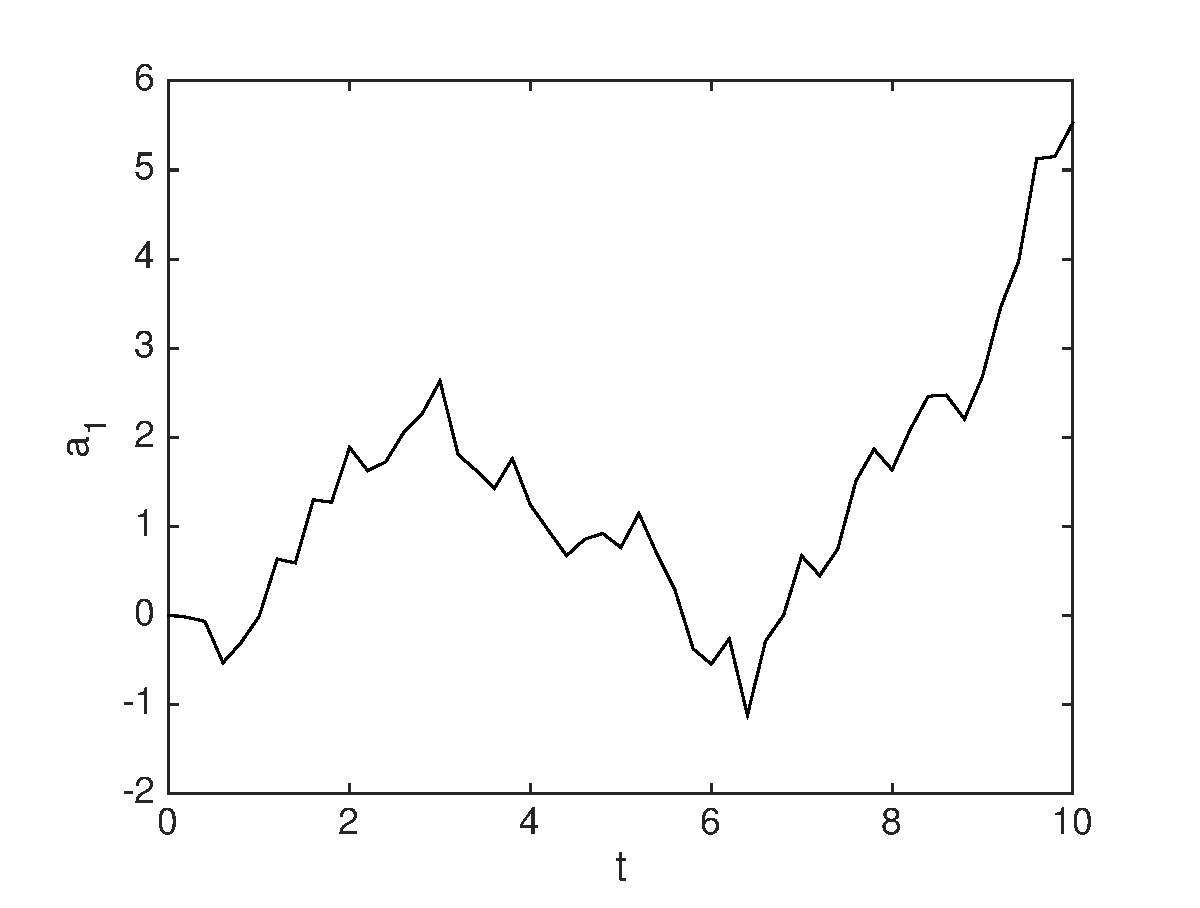
\includegraphics[width=0.75\textwidth]{Wiener_1}

\caption{\label{fig:The-simplest-case: Wiener}\emph{The simplest example:
a random walk.}}

\vspace{10pt}
 
\end{figure}
\par\end{center}

At the end of the run, xSPDE reports the RMS errors. There are discretization,
sampling and comparison errors, all normalized by the maximum observable
value, unless compared to a result of zero. In the present simulation,
the discretization or step error is about $10^{-16}$, due to round-off.
This is just a single trajectory, but more can be added.

\subsection{General derivatives}

All important xSPDE procedures use functions. Functions can be specified
inline, which is the simplest, or externally. The last argument of
any xSPDE function is the parameter structure. An example already
introduced is the derivative function, labeled $p.deriv$.

For example, consider the stochastic differential equation, 
\begin{equation}
\frac{da}{dt}=-ga+w.
\end{equation}
The corresponding derivative code definition is: 
\begin{center}
\doublebox{\begin{minipage}[t]{0.75\columnwidth}%
\texttt{p.deriv = @(a,w,p) - p.G{*}a + w;}%
\end{minipage}} 
\par\end{center}

This code defines the function handle $p.deriv$, which gives the
derivative function, $da/dt$. In this example, it simply returns
the derivative, in terms of the variable $a$, loss parameter $p.G$,
and stochastic noise term $w.$ This user specified inline function
is known internally by the function handle $p.deriv$.

Inside a complete xSPDE simulation input with a parameter values,
it would look like: 
\begin{center}
\doublebox{\begin{minipage}[t]{0.75\columnwidth}%
\texttt{p.G = 0.25;}

\texttt{p.deriv = @(a,w,p) - p.G{*}a + w;}

\texttt{xspde(p);}%
\end{minipage}} 
\par\end{center}

External function handles can also be used. They are useful for complex
functions with more internal logic.

A typical script first defines parameters and function specifications,
in a structure, then runs the simulation code with the parameter structure
as an input, as follows: 
\begin{center}
\doublebox{\begin{minipage}[t]{0.75\columnwidth}%
\texttt{p.{[}label1{]} = {[}parameter1{]};}

\texttt{...}

\texttt{p.{[}label2{]} = {[}parameter2{]};}

\texttt{p.deriv = @(a,w,p) {[}derivative{]};}

\texttt{xspde(p);}%
\end{minipage}} 
\par\end{center}

Note the following points to remember: 
\begin{itemize}
\item $\mathtt{p.}[label1]=[parameter1]$ defines a parameter in the structure
$p$. 
\item There are many possible inputs, which all have default values. 
\item You don't have to save the data if you want an immediate plot. 
\item The notation $\mathtt{p.deriv=}\mathtt{@(a,w,p)}\,\,[derivative]$
defines a function, $da/dt$. 
\item In this example, $\mathtt{a}$ is the stochastic variable, $\mathtt{w}$
the random noise, $p$ a structure. 
\item Other labels can be used instead of \emph{(a,w,p)} if preferred. 
\end{itemize}

\section{Input parameters\label{sec:Input-parameters}}

All xSPDE simulations use a structure for input data. Most functions
also require a parameter structure, combining the data input with
additional internal parameters. Any naming convention will do for
either structure, as long as you are consistent.

User-defined parameters can be added freely. To ensure that there
is no clash with internal variables, it is best if user defined parameters
start with a capital letter.

The xSPDE inputs have default values, which are used if the input
values are omitted. If you only need the first element of a vector
or array, just input the value required. Parameters can be output
with the verbose switch, \texttt{p.verbose}. This has four levels
of output: $-1$,$0$, $1$ or $2$, with \texttt{p.verbose=0} as
default, giving final error reports. To get more progress details
and individual errors, use \texttt{p.verbose=1.} To eliminate almost
everything, use \texttt{p.verbose=-1.} For maximum information, including
all the internal parameter values, use; 
\begin{center}
\doublebox{\begin{minipage}[t]{0.75\columnwidth}%
\texttt{p.verbose = 2;}%
\end{minipage}} 
\par\end{center}

While this level of detail is not usually needed, it can be useful
to print out all the internal parameters and default values to understand
how the program operates.

\subsection{Simulation parameters table\label{subsec:Simulation-parameters-1}}

The most common xSPDE input parameters used to define the equations
in a simulation, together with their default values are: \\

\begin{center}
\begin{tabular}{|c|c|c|c|}
\hline 
Label  & Type  & Default value  & Description\tabularnewline
\hline 
\hline 
\emph{fields}  & integer vector  & $1$  & Number of stochastic \emph{fields}\tabularnewline
\hline 
\emph{noises}  & integer vector  & $1$  & Number of \emph{noises}\tabularnewline
\hline 
\emph{name}  & string  & ' '  & Simulation \emph{name}\tabularnewline
\hline 
\emph{deriv}  & function  & 0  & The stochastic \emph{deriv}ative\tabularnewline
\hline 
\emph{initial}  & function  & 0  & Function to \emph{initial}ize variables\tabularnewline
\hline 
\emph{method}  & function  & {[}see \ref{sec:Algorithms}{]}  & Integration \emph{method}\tabularnewline
\hline 
\emph{ensembles}  & integer vector  & {[}1,1,1{]}  & Stochastic \emph{ensemble} sizes\tabularnewline
\hline 
\emph{ranges}  & real vector  & {[}10{]}  & Time and space \emph{ranges}\tabularnewline
\hline 
\emph{points}  & integer vector  & {[}51{]}  & Output lattice \emph{points} in {[}t,x,y,z,..{]}\tabularnewline
\hline 
\emph{steps}  & integer  & $[1]$  & Intermediate \emph{steps} per time point\tabularnewline
\hline 
\emph{observe\{n\}}  & function  & \emph{a}  & \emph{Observ}able function for averages\tabularnewline
\hline 
\emph{compare\{n\}}  & function  & \emph{0}  & \emph{Compar}ison function for averages\tabularnewline
\hline 
\emph{binranges\{n\}\{m\}}  & vector  & {[}0{]}  & \emph{Bin}ning \emph{ranges} for probabilities\tabularnewline
\hline 
\end{tabular}
\par\end{center}

A more detailed explanation of these parameters is found below, and
a complete table is given in section \ref{sec:Simulation-parameters}.

\subsection{Graphics parameters}

The generated average data can be graphed using any graphics editors,
or else using the internal xGRAPH function defined for this purpose.
An xSPDE simulation can return many different averages. These are
defined in a cell array with indices in braces. The index is used
to address the output data produced.

For each index, one can define parameters that define the quantity
stored, together with corresponding graphics outputs. Some commonly
used options are:\\

\begin{center}
\begin{tabular}{|c|c|c|c|}
\hline 
Label  & Type  & Default value  & Description\tabularnewline
\hline 
\hline 
\emph{olabels\{n\}}  & string  & \emph{'a'}  & Observable label\tabularnewline
\hline 
\emph{transverse\{n\}}  & integer  & \emph{$0$}  & Transverse slices in time\tabularnewline
\hline 
\emph{transforms\{n\}}  & vector  & $0$  & Set to 1 for Fourier transforms in time\tabularnewline
\hline 
\emph{scatters\{n\}}  & integer  & \emph{$0$}  & Set to s for s scatter plots in the observable\tabularnewline
\hline 
\end{tabular}\\
\par\end{center}

The full definition of the options is given in the user guide in sections
\ref{sec:xSIM-parameters} and \ref{sec:xGRAPH-reference}, although
most will be clear from examples.

\section{Fields and noises}

Stochastic variables in an SDE are \emph{fields}, stored in a real
or complex matrix, $a(i,j)$. Here, $i$ is an internal field index,
while $e$ is the ensemble index. 
\begin{description}
\item [{fields}] gives the range of the first internal index. This is the
total number of SDE variables or fields. It has a default value of
$fields=1$. 
\item [{ensembles}] allows multiple trajectories to be integrated. This
has up to three components. The first component, \emph{ensembles(1),
}gives a vector of local trajectories, so $e=1,\ldots$\emph{ensembles(1)}.
The two other ensemble values specify serial or parallel processing,
as explained below. 
\item [{noises}] are noise dimensions, similar to \emph{fields}, and used
as $w(i,j),$ where the first noise index has $noises$ components.
The default value is $noises=fields$. 
\end{description}
In the example above, we could add the fields, dimensions, ensembles
and noises:

\doublebox{\begin{minipage}[t]{0.75\columnwidth}%
\texttt{p.fields = 1;}

\texttt{p.dimensions = 1;}

\texttt{p.noises = 1;}

\texttt{p.ensembles = 1;}%
\end{minipage}}

As these are all default values, this is superfluous in a simple case.
The full definition of ensembles as a vector is given below, and in
some cases uses the parallel toolbox in Matlab.

\subsection{Initial values, points and ranges}

Initial values are required to define any differential equation, and
in a numerical calculation one must also have a defined lattice. 
\begin{description}
\item [{initial}] The initial value is defined by a function\texttt{ $p.initial$}.
This must return either an initial vector of size \emph{fields}, or
else a random array of size $fields\times ensembles(1)$. The default
function simply returns zero. 
\item [{inrandoms}] are initial random number dimensions, similar to \emph{fields},
and used as $v(i,j),$ where the first random dimension has $randoms$
components. The default value is $randoms=noises$. Specifies the
first argument of the function\texttt{ $p.initial(v,p)$} as a real
Gaussian noise vector $v$ with unit variance. The same noise is used
when error-checking, so that changes are from the step-size, not from
random fluctuations. 
\item [{points}] The number of integration points. The default setting
is currently $51$. 
\item [{steps}] The number of integration steps used for each output time-step.
The default is $1$. 
\item [{ranges}] The total integration range in each dimension, the first
element being the maximum integration time $T$. The default setting
is currently $10$. 
\end{description}

\subsection{Observables$ $}
\begin{description}
\item [{observe}] is a cell array of functions of stochastic fields, each
defining an average. xSPDE expects a (named or anonymous) function
that takes two parameters, namely the field matrix $a$ and the input
structure $p$. The function must return a real or complex matrix
of dimension $(\ell,ensembles(1))$, where $\ell$ indexes over a
vector observable. xSPDE then averages over the second index, to calculate
the observable.\\
 To plot the variance, for example: 
\end{description}
\doublebox{\begin{minipage}[t]{0.75\columnwidth}%
\texttt{p.observe\{1\} = @(a,p) (a(1,:)-mean(a,2)).\textasciicircum 2;}%
\end{minipage}} 
\begin{description}
\item [{rawdata}] By setting \emph{p.rawdata=1} (see section \ref{sec:xSIM-parameters}),
one can also store every trajectory including both fine and coarse
time-step values, and but this is very memory-intensive for large
simulations. 
\item [{olabels}] is cell array of graph labels associated with each average,
although one can also define a function of the averages to be graphed
with this label. 
\end{description}
Observables are computed as a two-dimensional packed array, then unpacked
for storage, giving an array of dimension $(d1,dspacetime,ensembles(1))$.
Here $d1$ is the local observable dimension, so $d1=1$ for a scalar
observable. The space-time dimension is $dspacetime=1$ for an SDE,
otherwise a vector for a SPDE, and $ensembles(1)$ is the size of
the ensemble of trajectories computed in each processor. Once data
is averaged internally over $ensembles(1)$, further transforms of
the resulting averages are available.

\subsection{Using the dot}

All equations entered in xSPDE utilize the Matlab syntax. This is
designed to handle scientific or mathematical matrix and array-based
formulae. It has features to simplify matrix or array equations which
often require a 'dot' or a 'colon'. 
\begin{itemize}
\item Stochastic variables in xSPDE are matrices or arrays, where the last
index is used to treat parallel stochastic trajectories, for greater
efficiency. This requires use of the 'dot' notation to perform multiplication
inside equations. 
\item To multiply vectors, matrices or arrays element-wise, like $a_{ij}=b_{ij}c_{ij}$,
the notation $a=b.*c$ indicates that all the elements are multiplied.
This is used to speed up calculations in parallel. 
\item An equation in xSPDE can apply to many stochastic trajectories in
parallel. Using the dot shortens the equation, and it also means that
a fast parallel arithmetic will be used. The same principle holds
for larger arrays with spatial lattices, treated in in section \ref{sec:Simulating-an-SPDE}. 
\item Broadcasting occurs if one or more dimensions has a unit size. For
example, arrays of size (1,100) and (6,1) can be added or multiplied
to give a (6,100) matrix. 
\item A formula for a stochastic field may require you to address the first
index - which is the field component - and treat all the other elements
in parallel. To do this in a compact way, one may use the notation
$a(1,:)$, which indicates that all the subsequent index elements
are being addressed as well. 
\item For an an SPDE this can ``flatten'' a larger array into a matrix.
This requires care to make sure all the terms have the same dimensionality
as described in section \ref{sec:Simulating-an-SPDE}. xSPDE includes
routines to help this issue. 
\end{itemize}
In summary, whenever a formula combines multiplication operations
over spatial lattices or ensembles, \textbf{USE THE DOT}.

\section{Advanced random walk}

We now return to the random walk, but with some more advanced features:
\begin{equation}
\dot{a}=w(t)\,,
\end{equation}

This is integrated numerically and graphed with $N=points(1)$ points.
The first point stored is the initial value, so there are $N-1$ integration
steps, of length $dt=ranges(1)/(N-1)$. Numerical graphs have discrete
steps, and more detail is obtained if more time steps are used. The
default value is $N=51$, which is predefined in the $xpreferences$
file. This is adjustable by the user. It can also be changed for a
simulation, by inputting a new value of $points$.

\subsection{Simple xSPDE example}

Unless you type \emph{clear} first, any changes to the input structure
are additive; so in the exercises you should get the combination of
all the previous structure inputs as well as your new input. 
\begin{itemize}
\item \textbf{Run the complete xSPDE script of Example 1 in Matlab.} 
\end{itemize}
It is simple to cut and paste from an electronic file to the command
window. Be careful; pasting can cause subtle changes that may require
correction. Some generated characters may be invalid input characters,
and these will need retyping if this occurs.

You should get the output in Fig (\ref{fig:The-simplest-case: Wiener}). 
\begin{itemize}
\item \textbf{What do you see if you average over $10000$ trajectories
?} 
\end{itemize}
\begin{center}
\doublebox{\begin{minipage}[t]{0.75\columnwidth}%
\texttt{p.ensembles = 10000;}

\texttt{xspde(p);}%
\end{minipage}} 
\par\end{center}
\begin{itemize}
\item \textbf{What do you see if you plot the mean square distance? Note
that variances should increase linearly with $t$.} 
\end{itemize}
\begin{center}
\doublebox{\begin{minipage}[t]{0.75\columnwidth}%
\texttt{p.observe = @(a,p) a.\textasciicircum 2;}

\texttt{p.olabels = '\textless a\textasciicircum 2\textgreater
';}

\texttt{xspde(p);}%
\end{minipage}} 
\par\end{center}
\begin{itemize}
\item \textbf{What if you add a force that takes the particle back to the
origin?} 
\begin{equation}
\dot{a}=-a+w(t)\,,\label{eq: damped_path_with_noise}
\end{equation}
\end{itemize}
\begin{center}
\doublebox{\begin{minipage}[t]{0.75\columnwidth}%
\texttt{p.deriv = @(a,w,p) -a+w;}

\texttt{xspde(p);}%
\end{minipage}} 
\par\end{center}

The corresponding Fokker-Planck equation from Eq \eqref{eq:FPE} is:
\begin{equation}
\frac{\partial P\left(a\right)}{\partial t}=\left[\frac{\partial}{\partial a}+\frac{1}{2}\frac{\partial^{2}}{\partial a^{2}}\right]P\left(a\right).
\end{equation}
It is easy to verify that inserting this dynamical equation into Eq
\eqref{eq:moment_equn} gives the result: 
\begin{equation}
\frac{\partial}{\partial t}\left\langle a^{2}\right\rangle =1-2\left\langle a^{2}\right\rangle 
\end{equation}

\begin{itemize}
\item Solve for $\left\langle a^{2}\left(t\right)\right\rangle $ and use
xSPDE to compare the numerical and analytic solutions. The current
time is accessible as the parameter $p.t$. Can you explain the graph
differences? 
\end{itemize}

\section{Probability binning}

It is possible to graph probability densities of real observables
instead of averages, if $p.ensembles$ is large. This is achieved
by inputting the observable number and binning range:

\begin{equation}
p.binranges\{n\}=\{oa:ostep:ob\};
\end{equation}

If present, this returns probability density of the $n$-th observable
$o\{n\}$, through binning into ranges of width $ostep$ around the
centers of each bin, starting at $\text{\emph{oa}}$, and ending at
$ob$. The simulation returns a result of $1/ostep$ in the $j-th$
bin if the trajectory is inside the bin, so that $o(j)-ostep/2<o<o(j)+ostep/2$,
and zero otherwise. This gives a probability density on output, plotted
against time. Note that on graphing, an extra dimension is added for
the variable $o$. The probability density at \textit{ntimes} equally
spaced simulation times can be plotted with \textit{p.transverse\{n\}=ntimes}.

The probability can be plotted for any \emph{observe} function of
the stochastic variable.

\subsection{Multivariate probabilities}

The probability density is multivariate for vector observables. This
is possible because the binning ranges are stored in a cell array,
which may contain several bin vectors. If the observable $o\{n\}$
is two-dimensional, then one can input:

\begin{equation}
p.binranges\{n\}=\{oa(1):ostep(1):ob(1),oa(2):ostep(2):ob(2)\};
\end{equation}

On graphing, \emph{two} extra dimensions are added for the variable
$o$ in this case. The graphics program \emph{xGRAPH} will attempt
to graph them, but it is limited by graphical visualization constraints.
In general, an arbitrary observable dimension is possible, but this
is also limited by the sampling and memory, since the number of samples
per bin will decrease rapidly with dimensionality.

The graphics program extracts slices and windows of probabilities
if required. To plot the probabilities of two observables, one for
a range of $-5:5$ and the other for 0:25 for a range of 0:1, add
the following inputs before the \emph{xsim} or \emph{xspde} command: 
\begin{center}
\doublebox{\begin{minipage}[t]{0.75\columnwidth}%
p.\texttt{binranges\{1\} = \{-5:0.25:5\};}

p.\texttt{binranges\{2\} = \{0:0.5:25\};}%
\end{minipage}} 
\par\end{center}

In the case of a two-dimensional probability density, plotted against
time, there are a total of four graphics dimensions. That is, one
dimension for time, two for the observable dimensions, and one for
the probability itself. One can also plot how the probability density
changes in space for the case of a stochastic partial differential
equation, as described in section \ref{sec:Simulating-an-SPDE}.

\section{Auxiliary fields and noises}

In some problems, it is useful to access the noise terms, or functions
of the noises and their correlations with the fields at the same time.
This is handled in xSPDE with auxiliary fields or \emph{auxfields.}
These are fields that are functions of noise terms and the integrated
fields. The number of these is defined in the input structures using
the parameter \emph{p.auxfields,} which is arbitrary.

Auxiliary fields are calculated using a function \emph{p.define,}
which is similar to \emph{p.deriv}, except that it returns the current
value of the auxiliary field, not the derivative. These fields are
defined as the \emph{average} over the previous step in time of the
auxiliary function, including the noise term. This is essential in
calculating spectra, in order to eliminate systematic errors in Fourier
transforms.

More details on this are given in Section (\ref{sec:Time-domain-spectra}).
To access the auxiliary fields, one can compute any observable average
using a \emph{p.observe} function as usual, or else store the \emph{raw
}trajectories including auxiliary fields by setting \emph{p.rawdata=1}.
In either case, the auxiliary fields are appended to the integrated
fields by adding extra cells.\emph{ }

\subsection{Outputting the noise}

As a simple example, suppose one wishes to calculate the noise terms
and compare them with the field trajectories in a simple Wiener process.
Since there is now an extra cell for the auxiliary field in the define
function, it is passed as an additional field argument to the observe
function. The following code can be used:\\

\doublebox{\begin{minipage}[t]{0.75\columnwidth}%
\texttt{clear}

\texttt{p.auxfields = 1;}

\texttt{p.deriv = @(a,w,p) w;}

\texttt{p.define = @(a,w,p) w;}

\texttt{p.observe = @(a,x,p) {[}a;x{]};}

\texttt{p.olabels = \{'a, w'\};}

\texttt{xspde(p);}%
\end{minipage}} \\

The observe function calculates both rows of the output array, including
the auxiliary field which is defined as the noise term and plotted
as a dashed line. There is no ensemble averaging, and hence no ensemble
error-bars in the example. This is because because no ensembles were
specified in the input parameters. Similarly, there are no time-step
error-bars for this observable, because the fine and coarse noises
are equal to each other after time averaging.

The result that is plotted is therefore the coarse noise, whose correlation
time equals the time step. This is plotted below in Fig ( \ref{fig:The-simplest-case: Wiener-2}),
which plots the same Wiener process as before, except adding the driving
noise term as well. The standard deviation of the noise in a single
step here is $\sqrt{1/dt}$, where $1/dt=50/10=5$ for the default
range of $10$ and default time points of $51.$ Note that noise terms
do not converge at small time-steps for delta-correlated noise, even
when the integrated stochastic process does converge. This is why
it is necessary to choose to plot one or the other, or else to time-average
to obtain a converged result.

If multiple steps are used, only the noise during the last step prior
to the time-point is plotted. 
\begin{center}
\begin{figure}
\centering{}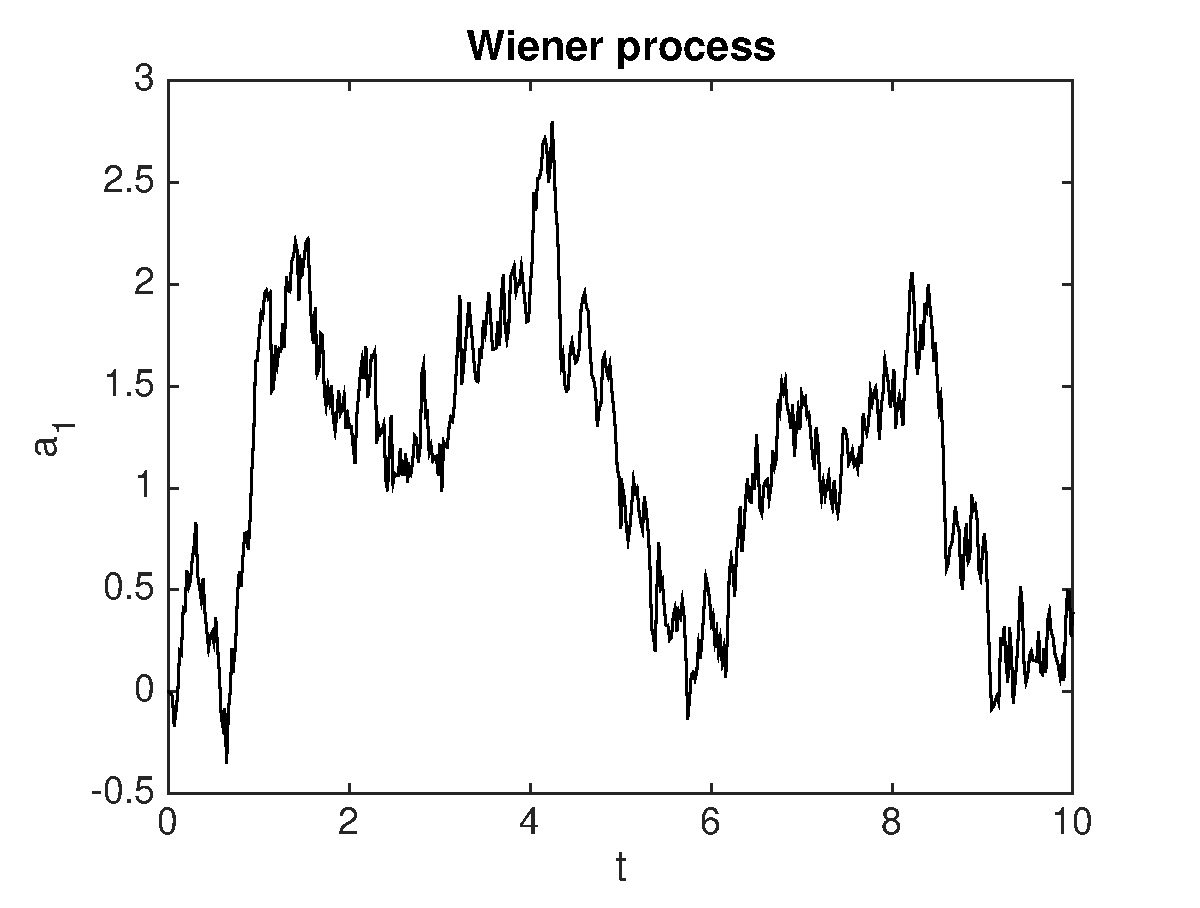
\includegraphics[width=0.75\textwidth]{Wiener_2}

\caption{\label{fig:The-simplest-case: Wiener-2}\emph{A single trajectory
of a random walk, with the noise terms $w$ graphed using dashed lines,
and the integrated variable $a$ plotted as the solid line.}}
\vspace{10pt}
 
\end{figure}
\par\end{center}

\section{Time-domain spectra\label{sec:Time-domain-spectra}}

To get an output from a temporally Fourier transformed field, set
$transforms\{n\}=1$ for the observable ($n$) you need to calculate
in transform space. This parameter is a cell array. It can have a
different value for every observable and for every dimension in space-time,
if you have space dimensions as well.

To obtain spectra from Eq \eqref{eq:field-average} with greater accuracy,
all fields are must be averaged internally. The code will use trapezoidal
integration in time over the integration interval, to give the average
midpoint value. This employs the same interval for fine and coarse
integration, to allow comparisons for error-checking. After this,
the resulting step-averaged fields are then Fourier transformed.

In the simplest case of just one internal step, with no error-checking,
this means that the field used to calculate a spectrum is: 
\begin{equation}
\begin{split}\bar{a}_{j}=\left({a}_{j}+{a}_{j+1}\right)/2,\end{split}
\end{equation}
which corresponds to the time in the spectral Fourier transform of:
\begin{equation}
\begin{split}\bar{t}_{j}=\left({t}_{j}+{t}_{j+1}\right)/2.\end{split}
\end{equation}

Note that if any temporal Fourier transform is specified, all the
field variables are time-averaged over a step. This is not strictly
necessary, but it means that there is a reduced code complexity for
cases where there is a Fourier transform for some but not all variables.
As described above, the auxiliary variables are always time-averaged
to allow error-checking, so there is no change for these.

\subsection{Error-checking}

For an error-checking calculation with two internal \emph{steps},
there are three successive valuations: $a_{j}$, $a_{j+1/2}$, $a_{j+1}$.
In this case, for spectral calculations one averages according to:
\begin{equation}
\begin{split}\bar{a}_{j}=\left(a_{j}+2a_{j+1/2}+a_{j+1}\right)/4.\end{split}
\end{equation}

In addition, one must define the noise terms, both for error-checking
and for output, since spectral calculations in quantum input-output
theory include noise terms as well as fields. The noise term used
to calculate a spectrum involving $\bar{a}_{j}$ is $w_{j}$. A coarse
noise term is set equal to the average of two successive fine noise
terms: 
\begin{equation}
\begin{split}\bar{w}_{1}=\frac{1}{2}\left(w_{1}+w_{1/2}\right).\end{split}
\end{equation}
The time integral is carried out numerically as a sum which has $N=points(1)$
time points of interval $dt$. In xSPDE, $dt=T/(N-1)$, where $T=ranges(1)$.
The effective integration time for the Fourier transform time integrals
is 
\begin{equation}
T_{eff}=Ndt=2\pi/d\omega
\end{equation}

When there are larger numbers of steps from using the internal \emph{steps}
parameter, there are more points to Fourier transform. These additional
frequencies are computed while carrying out the Fourier transform,
but only $N$ low frequency points are saved. The unused high frequency
results are not stored or plotted, to conserve memory.

\section{Examples}

\subsection{Complex damped spectrum}

Consider the spectrum of Eq \eqref{eq: damped_path_with_noise}, with
a complex noise, 
\begin{equation}
\left\langle w\left(t\right)w^{*}\left(t'\right)\right\rangle =\delta\left(t-t'\right),
\end{equation}
a random initial equation near the equilibrium value, and a range
of $t=100$, with $640$ points. Here there are two real noises.

The input parameters are given below. There are parallel operations
here, for ensemble averaging, so we \textbf{USE THE DOT}. 
\begin{center}
\doublebox{\begin{minipage}[t]{0.75\columnwidth}%
\texttt{clear}

\texttt{p.points = 640;}

\texttt{p.ranges = 100;}

\texttt{p.noises = 2;}

\texttt{p.ensembles = 10000;}

\texttt{p.initial = @(v,p) (v(1,:)+1i{*}v(2,:))/sqrt(2);}

\texttt{p.deriv = @(a,w,p) -a + w(1,:)+1i{*}w(2,:);}

\texttt{p.observe = @(a,p) a.{*}conj(a);}

\texttt{p.transforms = 1;}

\texttt{p.olabels = '\textbar a(\textbackslash omega)\textbar\textasciicircum 2';}

\texttt{xspde(p);}%
\end{minipage}} 
\par\end{center}

Note that \emph{p.}\texttt{\emph{transforms = 1}} tells xSPDE to Fourier
transform the field over the time coordinate before averaging, to
give a spectrum. Both \emph{observe} and \emph{transforms} could be
cell arrays, but the this is not needed with a single observable.
The first argument $v$ of the \emph{initial} function is a random
field, used to initialize the stochastic variable.

To define as many observables as you like, use a Matlab cell array; 
\begin{center}
\doublebox{\begin{minipage}[t]{0.75\columnwidth}%
\texttt{p.observe\{1\} = ..;}

\texttt{p.observe\{2\} = ..;}%
\end{minipage}} 
\par\end{center}

To learn more, try the following: 
\begin{itemize}
\item \textbf{Simulate over a range of $t=200$. What changes do you see?
Why?} 
\item \textbf{Change the equation to the laser noise equations introduced
in the next section (Laser quantum noise). Why is the spectrum much
narrower?} 
\end{itemize}

\subsection{Laser amplification noise}

Laser quantum noise is commonly modeled \cite{Louisell1973Quantum,Carmichael2002Statistical,gardiner2004quantum}
using SDEs in a normally ordered quantum phase-space representation.
Consider a model for the quantum noise of a single mode laser as it
turns on, near threshold:

\begin{equation}
\dot{a}=ga+bw(t)
\end{equation}
where the noise is complex, $w=\left(w_{1}+iw_{2}\right)$, so that:
\begin{equation}
\left\langle w(t)w^{*}(t')\right\rangle =2\delta\left(t-t'\right)\,.
\end{equation}

Here the coefficient $b$ describes the quantum noise of the laser,
and is inversely proportional to the equilibrium photon number.

Try the following, noting that you should type \emph{clear }first
when starting new simulations. 
\begin{itemize}
\item \textbf{Solve for the case of $g=0.1$, $b=0.01$} 
\end{itemize}
Most lasers have more than $100$ photons and hence much less noise
than this.

For this exercise, small error-bars will display on the graph. These
are calculated from the difference between using steps of size $dt$
and steps of size $dt/2$. They only appear if greater than a minimum
relative size, typically $1\%$ of the graph size, which can be set
by the user. 
\begin{center}
\doublebox{\begin{minipage}[t]{0.75\columnwidth}%
\texttt{clear}

\texttt{p.noises = 2;}

\texttt{p.observe = @(a,p) abs(a)\textasciicircum 2;}

\texttt{p.olabels = '\textbar a\textbar\textasciicircum 2';}

\texttt{p.deriv = @(a,w,p) a + 0.01{*}(w(1)+1i{*}w(2));}

\texttt{xspde(p);}%
\end{minipage}} 
\par\end{center}

\subsection{Saturated laser noise}

Consider the case where the laser saturates to a steady state:

\begin{equation}
\dot{a}=\left(1-\left|a\right|^{2}\right)a+bw(t)
\end{equation}

To learn how to use the function inputs, try the following: 
\begin{itemize}
\item \textbf{Solve for the saturated laser case} 
\end{itemize}
You should get the output graph in Fig (\ref{fig:The-laser}). 
\begin{center}
\doublebox{\begin{minipage}[t]{0.75\columnwidth}%
\texttt{p.deriv = @(a,w,p) (1-abs(a)\textasciicircum 2){*}a+0.01{*}(w(1)+1i{*}w(2));}

\texttt{xspde(p);}%
\end{minipage}} 
\par\end{center}

\begin{figure}
\centering{}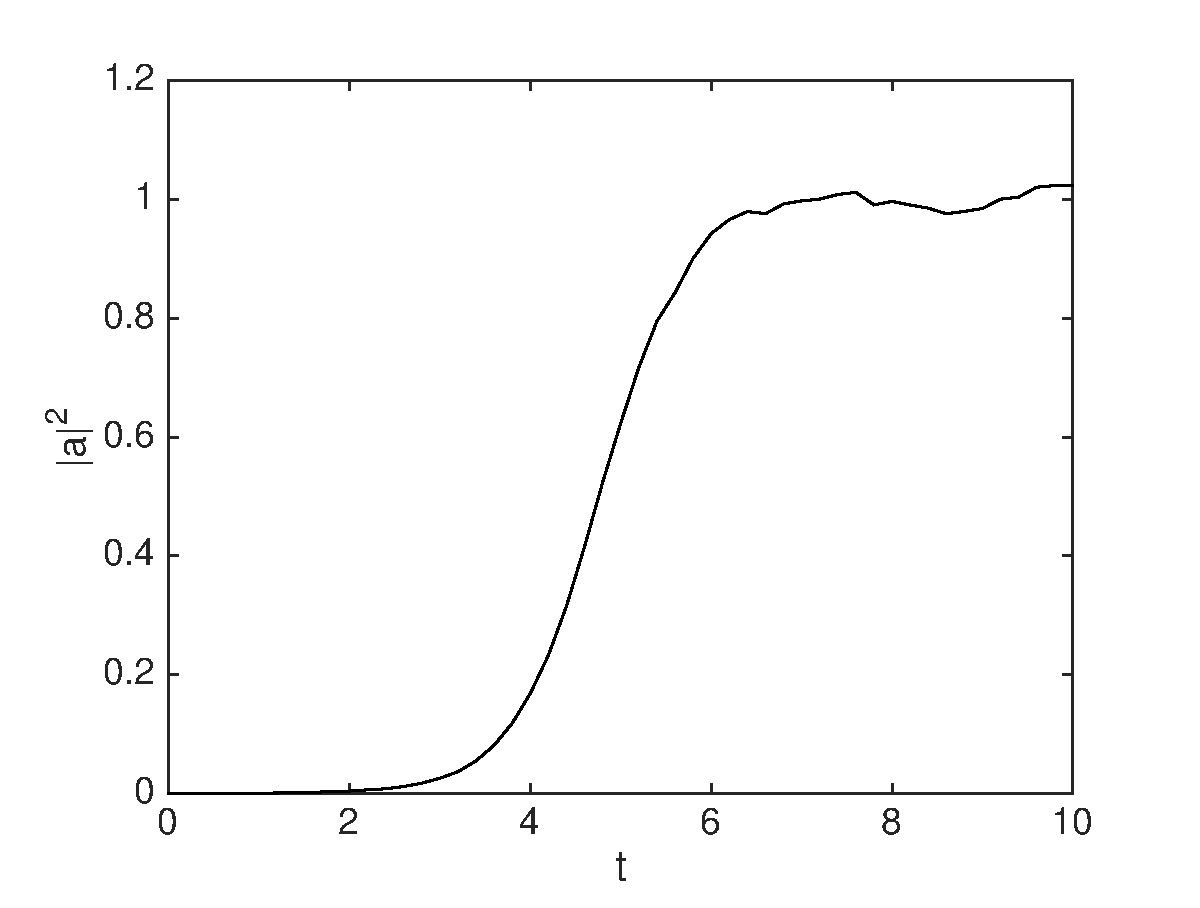
\includegraphics[width=0.75\textwidth]{Laser}

\caption{\label{fig:The-laser}\emph{Simulation of the stochastic equation
describing a laser turning on.}}
\vspace{10pt}
 
\end{figure}


\subsection{Financial calculus}

A well-known Ito-type stochastic equation is called the Black-Scholes
equation \cite{black1976pricing}, used to price financial options.
It describes the fluctuations in a stock or commodity value: 
\begin{equation}
da=\mu a\,dt+a\sigma\,dw,
\end{equation}
where $\left\langle dw^{2}\right\rangle =dt$. As the noise is multiplicative,
the equation is different in Ito and Stratonovich calculus. The corresponding
Stratonovich equation, as used in xSPDE for the standard default integration
routine is: 
\begin{equation}
\dot{a}=\left(\mu-\sigma^{2}/2\right)a+a\sigma w(t).
\end{equation}

An interactive xSPDE script in Matlab is given below with an output
graph in Fig (\ref{fig:The-Black-Scholes}). This is for a startup
with a volatile stock having $\mu=0.1,\,\sigma=1$. The spiky behavior
is typical of multiplicative noise, and also of the more risky stocks
in the small capitalization portions of the stock market. 
\begin{center}
\doublebox{\begin{minipage}[t]{0.75\columnwidth}%
\texttt{clear}

\texttt{p.initial = @(v,p) 1;}

\texttt{p.deriv = @(a,w,p) -0.4{*}a+a.{*}w;}

\texttt{xspde(p);}%
\end{minipage}} 
\par\end{center}

\begin{figure}
\centering{}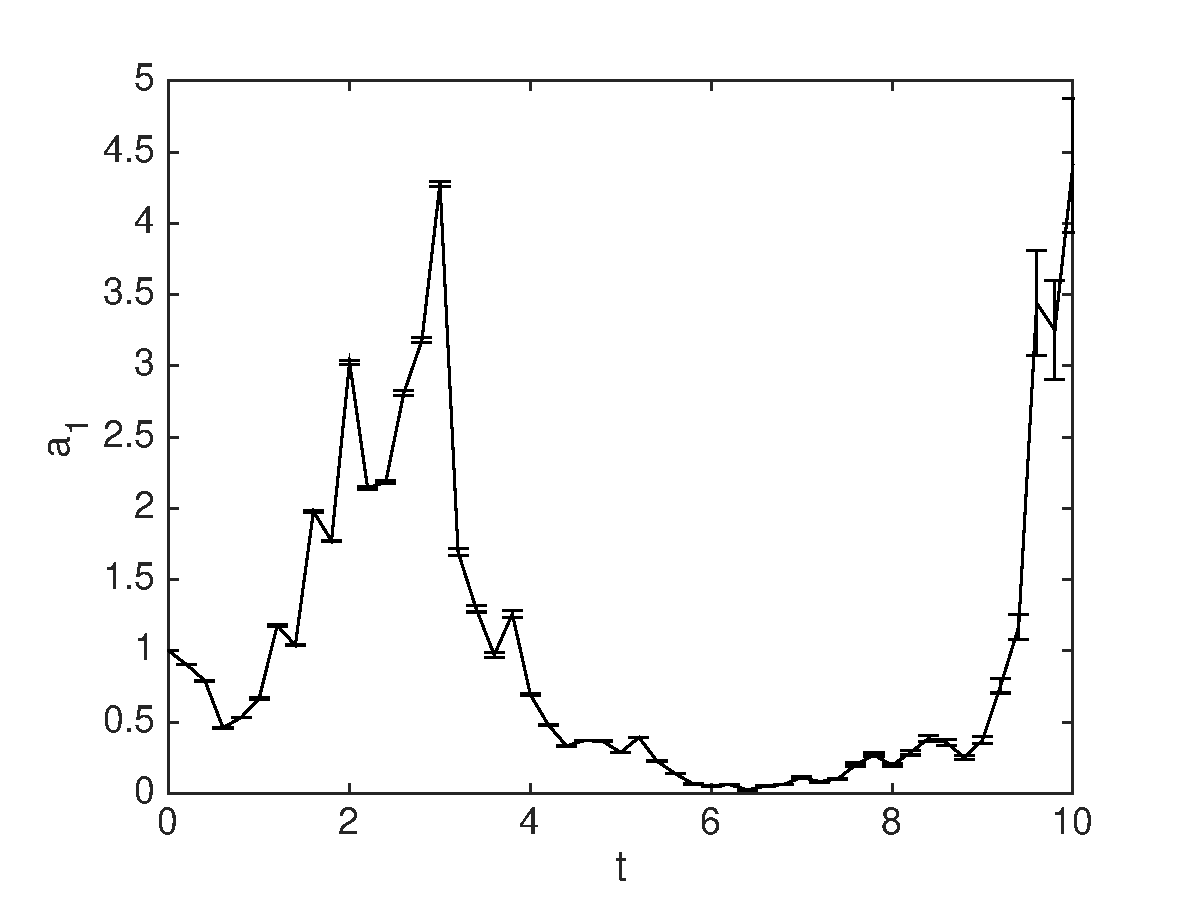
\includegraphics[width=0.75\textwidth]{Black-Scholes}

\caption{\label{fig:The-Black-Scholes}\emph{Simulation of the Black-Scholes
equation describing stock prices.}}
\vspace{10pt}
 
\end{figure}

Here $p.initial$ describes the initialization function. The first
argument of $@(v,p)$ is $v$, an initial random variable with unit
variance. \emph{The error-bars are estimates of step-size error}.
Errors can be reduced by using more time-steps.

To learn more, try the following: 
\begin{itemize}
\item \textbf{Solve for a more mature stock having $\mu=0.1,\,\sigma=0.1$.} 
\end{itemize}

\subsection{Nonlinear quantum simulation}

This example involves a full nonlinear quantum phase-space simulation
using the positive-P representation described in Sec (\ref{sec:Quantum-phase-space-equations}),
in which the two variables are only conjugate in the mean. This allows
quantum superpositions of coherent states to be represented, or in
fact any state, including squeezed or entangled states in more general
cases.

A simple example is the nonlinear driven quantum subharmonic generator
- for example, an opto-mechanical, superconducting or nonlinear optical
medium in a driven cavity \cite{Drummond1981Non-equilibrium,Sun2019Schrodinger,sun2019discrete,Lugiato1988Bistability}.
This is derived from the Hamiltonian for a resonant, coupled two-mode
nonlinear interferometer, with $\hat{a}_{2}$ driven externally at
twice the frequency of $\hat{a}_{1}$: 
\begin{equation}
\hat{H}=i\hbar\left[\frac{\kappa}{2}\hat{a}_{2}\hat{a}_{1}^{\dagger2}+\mathcal{E}_{2}\hat{a}_{2}^{\dagger}-h.c.\right]
\end{equation}

After including losses in both modes in the positive P-representation,
assuming zero temperature reservoirs, and adiabatically eliminating
$\alpha_{2}$ with $\gamma_{2}\gg\gamma_{1}$, one has the following
Ito equation: 
\begin{align}
\frac{d\alpha_{1}}{dt} & =-\gamma_{1}\alpha_{1}+\alpha_{1}^{\dagger}\frac{\kappa\epsilon_{2}}{\gamma_{2}}\left[1-\frac{\kappa}{2\epsilon_{2}}\alpha_{1}^{2}\right]+\sqrt{\frac{\kappa\epsilon_{2}}{\gamma_{2}}-\frac{\kappa^{2}}{2\gamma_{2}}\alpha_{1}^{2}}w_{1}\left(t\right)\nonumber \\
\frac{d\alpha_{1}^{\dagger}}{dt} & =-\gamma_{1}\alpha_{1}^{\dagger}+\alpha_{1}\frac{\kappa\epsilon_{2}}{\gamma_{2}}\left[1-\frac{\kappa}{2\epsilon_{2}}\alpha_{1}^{\dagger2}\right]+\sqrt{\frac{\kappa\epsilon_{2}}{\gamma_{2}}-\frac{\kappa^{2}}{2\gamma_{2}}\alpha_{1}^{\dagger2}}w_{1}\left(t\right)
\end{align}
Rescaling the fields so that $\alpha_{1}=a_{1}\sqrt{n_{c}}$, $\alpha_{1}^{\dagger}=a_{2}\sqrt{n_{c}}$,
where $n_{c}=\frac{2\epsilon_{2}}{\kappa}$, then rescaling time by
letting $\tau=\frac{\kappa\epsilon_{2}}{\gamma_{2}}t$, defining $c=\frac{\gamma_{1}\gamma_{2}}{\kappa\epsilon_{2}}$,
and using Eq (\ref{eq:ItovsStratonovichDrift}) to transform from
an Ito to a Stratonovich equation gives: 
\begin{align}
\frac{da_{1}}{d\tau} & =-(c-\frac{1}{2n_{c}})a_{1}+a_{2}\left[1-a_{1}^{2}\right]+\frac{1}{\sqrt{n_{c}}}\sqrt{1-a_{1}^{2}}w_{1}\left(\tau\right)\nonumber \\
\frac{da_{2}}{d\tau} & =-(c-\frac{1}{2n_{c}})a_{2}+a_{1}\left[1-a_{2}^{2}\right]+\frac{1}{\sqrt{n_{c}}}\sqrt{1-a_{2}^{2}}w_{2}\left(\tau\right)\,,
\end{align}
where $w_{1},w_{2}$ are delta-correlated real Gaussian noises.

There is a bistable region, which leads to a discrete time symmetry
breaking. The solution in the steady-state is 
\begin{equation}
P=\left(1-a_{1}^{2}\right)^{cn_{c}-1}\left(1-a_{2}^{2}\right)^{cn_{c}-1}e^{2n_{c}a_{1}a_{2}}
\end{equation}

The integration manifold is the region of real $a_{1}$, $a_{2}$,
such that $a_{1}^{2}\le1$ , $a_{2}^{2}\le1$. There are two physically
possible metastable values of the amplitudes. The physically observed
quantity is the amplitude and number: 
\begin{align}
\left\langle \hat{a}\right\rangle  & =\left\langle a_{1}+a_{2}\right\rangle \sqrt{\frac{n_{c}}{2}}\nonumber \\
\left\langle \hat{n}\right\rangle  & =n_{c}\left\langle a_{1}a_{2}\right\rangle .
\end{align}

Parameters that show bistable behavior on reasonable time-scales of
$T=100$ are $c=0.6$, $n_{c}=4$. To learn more, try the following: 
\begin{itemize}
\item \textbf{Simulate the nonlinear oscillator by creating a file, say,
$NonlinearQ.m$} 
\item \textbf{Can you observe quantum tunneling in the bistable regime?} 
\item \textbf{Do you see transient Schrödinger `cat states' with a negative
$n=\alpha_{1}\alpha_{2}$ value?} 
\end{itemize}
A negative value of $\alpha_{1}\alpha_{2}$ is evidence for a quantum
superposition! For experimental comparisons, one would measure correlation
functions and spectra. These calculations require long time scales,
$\mathtt{p.ranges}$, to observe tunneling, and of order $100$ time
steps per plotted time point, $\mathtt{p.steps}$, to maintain good
accuracy in the quantum simulations.

For lower damping and large nonlinearity, other methods should be
used, as the stochastic equations can become unstable in this limit.

The model is a simplified version of more recent quantum technologies
used to investigate Schrödinger cat formation in superconducting quantum
circuits \cite{leghtas2015confining}, and the CIM machine used to
solve NP-hard optimization problems with photonic circuits \cite{Marandi2014network,McMahon2019fully,Inagaki2019coherent},
although there are greater complexities in both these cases.

Similar methods can also be used to investigate quantum and chemical
non-equilibrium phase transitions \cite{drummond1981quasiprobability},
tunneling in open systems \cite{Kinsler1995Critical}, quantum entanglement
\cite{Kiesewetter2017Pulsed}, Einstein-Podolsky-Rosen paradoxes \cite{Reid1989Demonstration,Reid1989Correlations},
Bell violations \cite{RosalesZarate2014Probabilistic,Reid2014Quantum},
and many other problems treated in the literature \cite{gardiner2004quantum,Drummond2014Quantum}.

\section{Hints}
\begin{itemize}
\item When first using xSPDE, it is a good idea to run the batch test script,
\emph{Batchtest}. 
\item \emph{Batchtest} uses the Matlab parallel toolbox installation. If
you have no license for this, omit the third ensemble setting. 
\item To create a project file, it is often easiest to start with an existing
example function using a similar equation: see the xAMPLES folder. 
\item Graphics parameters can be included in the xSIM inputs to modify graphs. 
\item Comparison functions can be included if you want to compare with analytic
results. 
\item Chapters \ref{sec:xSIM-reference} and \ref{sec:xGRAPH-reference}
list the input parameters. 
\end{itemize}
\newpage{}

\chapter{Quantum toolbox \label{sec:Solving-an-SSE-2}}

\textbf{\emph{This chapter describes how to use the xSPDE numerical
toolbox to solve quantum dynamical problems.}}

Techniques for master equations and stochastic Schrödinger equations
(SSEs) are similar to those for an SDE, except for specific equations
that generate the derivatives, and a projected version of the stochastic
method.

The fundamental master equation solved has the Markovian form: 
\begin{align}
\dot{\rho} & =-i\left[\hat{H},\rho\right]+\sum_{j}\gamma_{j}\left(2\hat{L}_{j}\rho\hat{L}_{j}^{\dagger}-\hat{L}_{j}^{\dagger}\hat{L}_{j}\rho-\rho\hat{L}_{j}^{\dagger}\hat{L}_{j}\right),
\end{align}
where: $j=\left[j_{1},j_{2}(,j_{3})\right]$. Here $j_{1}$ is an
index that gives the type of damping operator, $j_{2}$ is a mode
index, and $j_{3}$ is an optional second mode index.

\section{Wave-functions and density matrices}

The quantum toolbox in xSPDE has three methods for representing open
quantum systems, which allow the treatment of Hilbert spaces of increasing
dimensionality: 
\begin{enumerate}
\item Density matrices with sparse operators 
\item Stochastic wave-functions with sparse operators 
\item Stochastic wave-functions with functional operators 
\end{enumerate}
There is a speed/memory tradeoff here. The lowest numbered methods
are typically faster, but use more memory. In the second two cases,
one can use either a method using functions for operators, or else
a sparse matrix method, which requires the operators to be stored
in memory. The wave-function equations describe decoherence through
stochastic methods, so each of these two approaches can treat coupling
to reservoirs, up to the limits of time and memory constraints.

When using sparse methods, the multimode index $\bm{n}$ is packed
into the first single index $n$. This is automatic for density matrices,
but it is optional for stochastic wave-function calculations, which
can use either sparse or full vectors. While sparse methods are useful
for storing operators, these require memory, which must be allocated
when the matrices are generated. This can be minimized by only generated
the operators that are needed, rather than all possible ones.

Less memory is required if the operators' effect on the wave-function
are calculated only when needed. This is a function call strategy,
It is currently available for stochastic wave-function calculations
only. It is slower than using sparse matrices, but it is more scalable.
Currently, this approach is not available for density matrix equations.

These different approaches therefore have areas of applicability that
depend on the Hilbert space dimension, as explained below.

\subsection{Number-state methods}

Algorithms for either wave-functions or density matrices, are selected
by choosing two parameters, \emph{quantum} and \emph{sparse}. If \emph{sparse}
is omitted, the default is $sparse=0$. 
\begin{description}
\item [{p.quantum~=~1,~p.sparse~=~0}] - this is used to treat a full
wave-function, $psi(\bm{n},e)$, Here, $\bm{n}=n_{1},\ldots n_{m}$
is a wave-function index index, while $e$ is an ensemble index for
random ensembles, if used. Operators are treated as functions, so
there are no operator matrices stored. This minimizes the overall
memory requirement. 
\item [{p.quantum~=~1,~p.sparse~=~1}] - this is used to treat a packed
wave-function, $psi(n,e)$, Here, $n$ is a wave-function index index,
which is a packed version of the vector index $\bm{n}$, while $e$
is an ensemble index for random ensembles. Operators are treated as
sparse matrices, so these must be stored. This increases the overall
memory usage but is somewhat faster. 
\item [{p.quantum~=~2,~p.sparse~=~1}] - this is used to treat a packed
density matrix, $rho(n,\ell)$, Here, $n$ and $\ell$ are density
matrix indices, which are packed version of the vector index $\bm{n}$.
Operators are treated as sparse matrices. Due to the storage requirements
of a density matrix, this uses the most memory, and is the fastest.
There is no vector ensemble here. 
\end{description}

\subsection{Independent cells}

If one wishes to combine results from independent quantum systems,
or from classical and quantum subsystems, the relevant parameters
can be input as successive cell variables, together with any other
toolbox inputs that are required. This allows, as an example, implementation
of the Maxwell-Bloch equations, togther with arbitrary numbers of
independent quantum systems like molecules and atoms.

\section{Input parameters}

Input parameters are stored in a structure which is input to the \emph{xSPDE}
program. This is a superset of the parameters already defined. In
the definitions below, the structure name is omitted. but we normally
use $p$ in the examples. For example, to specify a quantum wave-function
method, one would use $quantum=1$, as explained already. The input
parameters can be chosen not just in terms of the problem itself,
but also to suit the computational hardware that is available.

Not that while the $quantum$ toolbox and $phase$ toolbox share common
parameters listed below, but they are distinct toolboxes, and one
must choose to use either one or the other by setting $quantum>0$
or $phase>0$.

\subsection{Common parameters}
\begin{description}
\item [{modes}] gives the number of modes, hence $modes=3$ defines a 3
mode quantum system,. This can be given implicitly through nmax. 
\item [{ensembles(1)}] gives a vector of trajectories, $e=1,\ldots$\emph{ensembles(1)}.
This is fast, but increases memory use. It is not used for density
matrices. 
\item [{ensembles(2)}] gives the number of series repeats for stochastic
ensembles. It is always available, but slower. 
\item [{ensembles(3)}] gives the number of parallel repeats for stochastic
ensembles. It is useful for multicore processors with fast memory. 
\item [{jump~-}] this selects either a continuous stochastic differential
equation (\emph{jump = 0}), the default, or a stochastic jump equation
(\emph{jump=}1). 
\item [{noises}] are noise dimensions., set automatically for the built-in
quantum methods. If other methods are used \emph{noises }may need
specifying. 
\item [{points}] The number of integration points in time for data outputs.
The default setting is $51$. 
\item [{steps}] The integration steps used per time-step, used to reduce
time-step errors. The default is $1$. 
\item [{ranges}] The total integration range in time. The default setting
is$10$. 
\item [{initial}] The initial state is given by a function\texttt{ $initial$}.
This returns a column vector of size \emph{$fields\times1$} or $fields\times ensembles(1)$,
for wave-functions, or else of size $fields\times fields$ for density
matrix calculations. The default is the state with the first level
occupied. 
\item [{inrandoms}] are initial random number dimensions. They specify
the first argument of the function\texttt{ $initial(v,p)$} as a real
Gaussian noise vector $v$ with unit variance and length \emph{inrandoms}.
These are used for an initially decoherent, randomized wave-function. 
\end{description}
The internal variable \emph{fields }is used to specify the dimension
of the integrated variables, and is automatically set.

\subsection{Quantum parameters }
\begin{description}
\item [{quantum}] is the type of problem: $quantum=1$ for a wave-function,
$quantum=2$ for a density matrix. 
\item [{sparse}] indicates sparseness: if $sparse=1$, sparse matrices
are used to store operators. The default is $sparse=0$. 
\item [{nmax}] is the Hilbert dimension per mode. If this is a vector,
the dimension can be varied. 
\item [{gamma}] is a cell array of functions that define an amplitude decay
rate. If omitted, these must be specified in the Lindblad operators. 
\item [{alpha}] is a cell array of amplitudes for the noise. type., to
allow different unravellings. If zero, there is a complex noise. 
\item [{L}] is a cell array of Lindblad operator functions for different
types of decoherence. 
\item [{mk...}] is a make function to generate sparse operators where required,
eg,\textbf{ mkbose}. 
\end{description}
Note the following defaults are used to simplify input: 
\begin{itemize}
\item If \emph{modes }is not specified, it is equal to the length of \emph{nmax}. 
\item If \emph{modes} and \emph{nmax} are not specified the default is a
single qubit\emph{: modes=1} , \emph{nmax=2}. 
\item If the \emph{nmax} vector is shorter than \emph{modes}, the last value
of \emph{nmax} is repeated as necessary. 
\end{itemize}

\section{Dissipative parameters}

In order to explain the terminology, the following list is useful.
There are some differences that depend on whether one uses sparse
matrices or functional operators to describe the quantum operators. 
\begin{description}
\item [{operator:}] If \emph{sparse=0}, an operator is a function with
inputs of the mode index (or indices), and the wave-function $psi$.
Operators acting on multiple modes may have two or more indices. The
function $O_{k}$ returns a wave-function $\hat{O}_{k}\left|\psi\right\rangle $. 
\item [{sparse\_operator:}] When \emph{sparse=1}, operators are sparse
matrices. This is faster, but uses more memory. 
\item [{Hamiltonian:}] the function $H(psi,p)$ returns a wave-function
$\hat{H}\left|\psi\right\rangle $, if \emph{sparse=0}. Otherwise,
if \emph{sparse=1}, it is an operator function $H(p)$ that returns
a sparse matrix. 
\item [{L\{n\}:}] this is a cell array of dissipative or ``Lindblad''
functions. The first argument is the mode index, $k$, or a vector
of two indices, $[k_{1},k_{2}]$, and the last argument p includes
parameters. 
\begin{description}
\item [{@(k,p)}] is used for sparse operators. The function returns a sparse
matrix $\hat{L}_{k}$. 
\item [{@(k,psi,p)}] is used for operator functions. The function can return
both $\hat{L}_{k}\left|\psi\right\rangle $, and $\hat{L}_{k}^{\dagger}\hat{L}_{k}\left|\psi\right\rangle $,
as required. 
\end{description}
\item [{gamma\{n\}(p):}] This is a cell array of functions for every type
of damping process. Cell array indices give different types of damping.
If used, it returns a vector or matrix of damping rates for each type
of Lindblad operator. If omitted, the rates must be included in the
operators. 
\item [{alpha\{n\}(k):}] This is a cell array of noise amplitude vectors
or matrices for each type of damping process with real noises. If
\textbf{alpha} is zero, which is the default, a complex noise is used. 
\end{description}
Note that: 
\begin{itemize}
\item Operators may have one or two mode indices. 
\item Functional operators are slower than sparse operators for small Hilbert
spaces. 
\item Only the required index combinations are accessed by the Lindblad
functions, reducing storage. 
\item A separate \emph{gamma} array is more efficient if some Lindblad indices
have a zero rate. 
\end{itemize}

\section{Functional operators}

These are linear functions that act on the quantum wave-function.
New ones can readily be added. They reduce memory requirements, which
is an advantage for large Hilbert spaces, where storing even sparse
operators can require large quantities of memory.

The xSPDE code includes internal functions for bosonic and spin operators.
The predefined operators also return auxiliary quantities used in
dissipative equations if required, as they have variable input and
output lists.

\subsection{Bosonic operators({*}PARTLY IMPLEMENTED)}
\begin{center}
\begin{tabular}{|c|c|c|}
\hline 
Label  & Inputs  & Output(s)\tabularnewline
\hline 
\hline 
\emph{a}  & \emph{$(m,psi)$}  & $\hat{a}_{m}\left|\psi\right\rangle $\tabularnewline
\hline 
\emph{ad}  & \emph{$(m,psi)$}  & $\hat{a}_{m}^{\dagger}\left|\psi\right\rangle $\tabularnewline
\hline 
\emph{a2}  & \emph{$([m,n],psi)$}  & $\hat{a}_{m}\hat{a}_{n}\left|\psi\right\rangle $\tabularnewline
\hline 
\emph{ad2}  & \emph{$([m,n],psi)$}  & $\hat{a}_{m}^{\dagger}\hat{a}_{n}^{\dagger}\left|\psi\right\rangle $\tabularnewline
\hline 
\emph{n}  & \emph{$([m,n],psi)$}  & $\hat{a}_{m}^{\dagger}\hat{a}_{n}\left|\psi\right\rangle $\tabularnewline
\hline 
\emph{n2}  & \emph{$([m,n],psi)$}  & $\hat{n}_{m}\hat{n}_{n}\left|\psi\right\rangle $\tabularnewline
\hline 
\end{tabular}
\par\end{center}

Nonlinear operators can have up to two indices. For a complete description,
see (\ref{subsec:Bosonic-operator-table}).

\subsection{Qubit and Pauli spin operators({*}PARTLY IMPLEMENTED)}

The following set of operators are used for spin chain evolution. 
\begin{center}
\begin{tabular}{|c|c|c|}
\hline 
Label  & Inputs  & Output(s)\tabularnewline
\hline 
\hline 
\emph{sx}  & \emph{$(m,psi)$}  & $\hat{\sigma}_{m}^{x}\left|\psi\right\rangle $\tabularnewline
\hline 
\emph{sy}  & \emph{$(m,psi)$}  & $\hat{\sigma}_{m}^{y}\left|\psi\right\rangle $\tabularnewline
\hline 
\emph{sz}  & \emph{$(m,psi)$}  & $\hat{\sigma}_{m}^{z}\left|\psi\right\rangle $\tabularnewline
\hline 
\emph{sx2}  & \emph{$(m_{1},m_{2},psi)$}  & $\hat{\sigma}_{m_{1}}^{x}\hat{\sigma}_{m_{2}}^{x}\left|\psi\right\rangle $\tabularnewline
\hline 
\emph{sy2}  & \emph{$(m_{1},m_{2},psi)$}  & $\hat{\sigma}_{m_{1}}^{y}\hat{\sigma}_{m_{2}}^{y}\left|\psi\right\rangle $\tabularnewline
\hline 
\emph{sz2}  & \emph{$(m_{1},m_{2},psi)$}  & $\hat{\sigma}_{m_{1}}^{z}\hat{\sigma}_{m_{2}}^{z}\left|\psi\right\rangle $\tabularnewline
\hline 
\end{tabular}
\par\end{center}

\subsection{Qubit gate operators({*}PARTLY IMPLEMENTED)}

The following operators can be used to implement quantum logic gates,
in addition to the standard Pauli operators. These assume qubit or
two-state qubit logic in each mode. 
\begin{center}
\begin{tabular}{|c|c|c|}
\hline 
Label  & Inputs  & Output(s)\tabularnewline
\hline 
\hline 
\emph{cx}  & \emph{$(m_{1},m_{2},psi)$}  & Controlled Not\tabularnewline
\hline 
\emph{ha}  & \emph{$(m,psi)$}  & Hadamard\tabularnewline
\hline 
\emph{p8}  & \emph{$(m,psi)$}  & $\pi/8$\tabularnewline
\hline 
\emph{ph}  & \emph{$(m,psi)$}  & Phase\tabularnewline
\hline 
\end{tabular}
\par\end{center}

\section{Sparse operators }

The xSPDE code includes internal functions to generate operators.
These are either sparse or full. Sparse operators are generated if
needed requiring a \emph{mk} function call to create the required
index combinations, before they are used.

\subsection{Sparse bosonic operators: \emph{mkbose.}}

These are a cell array of annihilation operators, generated using
\emph{mkbose.} 
\begin{center}
\begin{tabular}{|c|c|c|}
\hline 
Label  & Indices  & Meaning\tabularnewline
\hline 
\hline 
\emph{a}  & \emph{$\{m\}$}  & $\hat{a}_{m}$\tabularnewline
\hline 
\emph{a'}  & \emph{$\{m\}$}  & $\hat{a}_{m}^{\dagger}$\tabularnewline
\hline 
\end{tabular}
\par\end{center}
\begin{description}
\item [{p.a~=~mkbose((list,)~p)}] Returns a cell array of annihilation
operators defined either at all modes, if there is no \emph{list,
}or at the listed mode locations\emph{. }Here\emph{ list }is a vector
of integers, \emph{p} is the parameter structure. 
\end{description}

\subsection{Sparse Pauli spin operators: \emph{mkpauli.}}

The following set of operators are used for spin chain evolution.
They are generated using \emph{mkpauli.} 
\begin{center}
\begin{tabular}{|c|c|c|}
\hline 
Label  & Indices  & Meaning\tabularnewline
\hline 
\hline 
\emph{sx}  & \emph{$\{m\}$}  & $\hat{\sigma}_{m}^{x}$\tabularnewline
\hline 
\emph{sy}  & \emph{$\{m\}$}  & $\hat{\sigma}_{m}^{y}$\tabularnewline
\hline 
\emph{sz}  & \emph{$\{m\}$}  & $\hat{\sigma}_{m}^{z}$\tabularnewline
\hline 
\end{tabular}
\par\end{center}
\begin{description}
\item [{{[}p.sx,p.sy,p.sz{]}~=~mkpauli((list,)~p)}] Returns three cell
arrays of Pauli operators defined either at all modes, if there is
no \emph{list, }or at the listed mode locations\emph{. }Here\emph{
list }is a vector of integers, \emph{p} is the parameter structure. 
\end{description}

\subsection{Sparse logic operators({*}NOT IMPLEMENTED)}

The following operators can be used to implement quantum logic gates,
in addition to the standard Pauli operators. These assume qubit or
two-state qubit logic in each mode. They are generated using \emph{mklogic.} 
\begin{center}
\begin{tabular}{|c|c|c|}
\hline 
Label  & Inputs  & Output(s)\tabularnewline
\hline 
\hline 
\emph{cx}  & \emph{$\{[m,n]\}$}  & Controlled Not\tabularnewline
\hline 
\emph{ha}  & \emph{$\{m\}$}  & Hadamard\tabularnewline
\hline 
\emph{p8}  & \emph{$\{m\}$}  & $\pi/8$\tabularnewline
\hline 
\emph{ph}  & \emph{$\{m\}$}  & Phase\tabularnewline
\hline 
\end{tabular}
\par\end{center}
\begin{description}
\item [{{[}p.ha,p.p8,p.ph{]}~=~mklogic1((list,)~p)}] Returns three cell
arrays of unary logic operators defined either at all modes, if there
is no \emph{list, }or at the listed locations\emph{. }Here\emph{ list
}is a vector of integers, \emph{p} is the parameter structure. 
\item [{p.cx~=~mklogic2((list,)~p)}] Returns a cell array of binary
\emph{controlled not} operators defined either at all modes, if there
is no \emph{list, }or at the listed locations\emph{. }Here\emph{ list
}is a matrix of integers, \emph{p} is the parameter structure. 
\end{description}

\section{\emph{Observe}, \emph{expect, output }and\emph{ compare}}

There are four types of possible outputs. The \emph{observe} and \emph{compare}
functions are computed during the time-evolution, so that the entire
wave-function doesn't need to be stored in time, reducing the storage
needs. Additional functional transformations for either can be used
as well, called \emph{output} functions. Finally, a \emph{compare}
function allows comparison plots. 
\begin{description}
\item [{observe}] is a cell array of \emph{any} stochastic function. xSPDE
expects a (named or anonymous) function that takes two parameters,
namely the wave-function $psi$ or density matrix $\rho$, and the
input structure $p$. The function return a real or complex matrix
of dimension $(\ell,ensembles(1))$, where $\ell$ indexes a vector
observable. xSPDE then averages over the second index, to calculate
the observable. This allows an average of any type. 
\item [{expect}] is a cell array of operators defining a quantum expectation
value. For full matrices, \emph{expect} is a (named or anonymous)
function that takes two inputs, the wave-function $psi$ and the structure
$p$. For sparse matrices, the \emph{expect} function returns a matrix.
xSPDE internally averages over both the quantum and stochastic degrees
of freedom to calculate the observable.\\
 To plot the mean number in mode $m=1$, using:\\
 a) the number operator $\hat{n}=\hat{a}^{\dagger}\hat{a}$ with sparse
operators:\\
 ~~%
\doublebox{\begin{minipage}[t]{0.75\columnwidth}%
\texttt{p.expect\{1\} = @(p) p.a\{1\}'{*}p.a\{1\};}%
\end{minipage}}\\
 ~\\
 b) the number operator $\hat{n}=\hat{a}^{\dagger}\hat{a}$, with
function calls: \\
 %
\doublebox{\begin{minipage}[t]{0.75\columnwidth}%
\texttt{p.expect\{1\} = @(psi,p) n(1,psi);}%
\end{minipage}} 
\item [{output}] All \emph{observe} and \emph{expect} results are stored.
Transformations of both can be introduced. These may include multiple
averages and/or different times. These are called the \emph{output}
functions. Default \emph{outputs} pass through \emph{observe} and
\emph{expect} results with no change. Defined outputs, like \emph{p.output\{1\}},
replace the defaults, or add new outputs. Graphed data uses the \emph{outputs},
which include sampling errors if \emph{ensembles} are used, and step-size
errors if \emph{checks} is turned on. 
\item [{compare}] Comparison functions can be used to obtain comparison
graphs and differences. 
\end{description}
The output numbering that is used is the \textbf{same} for all four
types of function. This can lead to overwriting, with the precedence
that \emph{output\textgreater expect\textgreater observe}. To prevent
overwriting, use different cell-indices. Compare functions are plotted
independently, as an extra line on an existing graph, so they don't
overwrite, and can be compared with any of \emph{output, expect, observe.}

\section{SSE derivative}

The SSE derivative terms are calculated from two distinct derivative
subroutines, which are $SSElinear(a,w,p)$ for solving the linear
SSE, Eq (\ref{eq:linear_SSE}), and $SSE(a,w,p)$ for solving the
nonlinear SSE, Eq \ref{eq:nonlinear SSE}. Note that SSE is the default
if this is not specified.

These are specified in the nonlinear equation case by the input of:
\[
p.deriv=@SSE
\]
or, for the linear case, which is \emph{not} recommended except for
tutorial purposes(!) 
\[
p.deriv=@SSElinear.
\]

These correspond to normalized and un-normalized wave-functions. The
equation can be solved by any $method$ for a Stratonovich SDE. For
SSE, typically the lowest errors are obtained using an RK4 Schrödinger
method with projective normalization, @RK4S.

\section{Solving with the MCWF method \label{sec:Solving-with-MCWF-1}}

At each time step in the numerical simulation with the MCWF method,
the jump probability $\Delta P$ is first calculated. This is carried
out by computing the jump probability per unit time of each jump operator
$L_{m}$ in the master equation, which is given by 
\begin{equation}
\Delta P_{m}=2\gamma_{m}\langle\psi(t)|L_{m}^{\dagger}L_{m}|\psi(t)\rangle\,.\label{eq:individual_jump_prob-1}
\end{equation}

The calculated jump rate $\Delta P_{m}$ is then compared with a uniform,
randomly generated number $r_{m}$ between zero and $1/\Delta t$.
If $\Delta P_{m}>r_{m}$, the state then undergoes the given jump.
As $\Delta t\rightarrow0$, a jump in any given step become increasingly
rare.

After this, the state vector evolves according to the non-hermitian
Hamiltonian $H_{eff}$ in Eq. (\ref{eq:non-Hermitian_Hamiltonian})
as follows: 
\begin{equation}
\frac{d}{dt}|\psi(t)\rangle=-iH_{eff}|\psi(t)\rangle\label{eq:ODE-1}
\end{equation}
This differential equation is solved by a RK4S algorithm, or others
that are available. These steps are repeated till the final time step,
and they constitute a single trajectory. Many trajectories are taken
to compute the expectation values for the observables of interest.

For error-checking, fine step results are checked against a coarse
step with a noise given by $r_{c}=\min\left(r_{1},r_{2}\right)$,
so that the coarse jump occurs if a jump takes place in either fine
step. This allows errors due to step-size to be accurately estimated
by comparing the fine and coarse step-size results, just as with continuous
noise.

The MCWF algorithm described above is carried out simply by setting
$p.jump=1$. No further inputs from the user are required. All other
parameters are input exactly the same way as in the SSE numerical
simulation.

\newpage{}

\chapter{Phase-space toolbox \label{chap:Phase-space}}

\textbf{\emph{This chapter describes how to use the xSPDE numerical
toolbox to solve network and quantum dynamical problems in phase-space.}}

\section{Phase-spaces}

There are multiple phase-space methods available. These include the
classical Wigner, Husimi and Glauber representations, as well as the
positive-P and gauge methods. These are generally applicable to large
Hilbert spaces as well as small ones. They have other limitations,
and the reader is referred to the original literature to obtain further
explanations of these methods.

These different approaches therefore have areas of applicability that
depend on the Hilbert space dimension, as explained below.

\subsection{Phase-space methods}

These are used for phase-space mappings, selected by choosing three
relevant parameters, \emph{phase, number} and \emph{gauge}. When \emph{gauge}
and are omitted, the default is $gauge=0$. Details are: 
\begin{description}
\item [{p.phase~=~1}] - this is used to treat a normally-ordered P-representation
or positive P-representation. 
\item [{p.phase~=~2}] - this is used to treat a symmetrically-ordered
Wigner-representation. 
\item [{p.phase~=~3}] - this is used to treat an anti-normally-ordered
Q-representation. 
\item [{p.phase~=~1,~p.gauge~=~1}] - this is used to treat a normally-ordered
gauge P-representation, which includes an additional real or complex
weight. 
\item [{p.phase~=~1,~p.number~=~1}] - this is used to treat a normally-ordered
gauge P-representation using stochastic jumps, with additional output
of the number of jumps to allow a large-scale simulation of counting
statistics. 
\end{description}

\section{Input parameters}

Input parameters are stored in a structure which is input to the \emph{xSPDE}
program. This is a superset of the parameters already defined. In
the definitions below, the structure name is omitted. but we normally
use $p$ in the examples.

Not that while the $quantum$ toolbox and $phase$ toolbox share common
parameters listed below, they are distinct toolboxes, and one must
choose to use either one or the other by setting $quantum>0$ or $phase>0$.

\subsection{Common parameters}
\begin{description}
\item [{modes}] gives the number of modes, hence $modes=3$ defines a 3
mode quantum system. 
\item [{ensembles(1)}] gives a vector of trajectories, $e=1,\ldots$\emph{ensembles(1)}.
This is fast, but requires memory. It is not used for direct density
matrix simulations 
\item [{ensembles(2)}] gives the number of series repeats for stochastic
ensembles. It is always available, but slow. 
\item [{ensembles(3)}] gives the number of parallel repeats for stochastic
ensembles. It is useful for multicore processors with fast memory. 
\item [{noises}] are noise dimensions. There should be $1$ or $2$ real
noises per independent relaxation process in each mode, for real or
complex noise processes respectively. These are set automatically
if the built-in stochastic methods are used. 
\item [{points}] The number of integration points in time. The default
setting is $51$. 
\item [{steps}] The integration steps used per time-step. The default is
$1$. 
\item [{ranges}] The total integration range in time. The default setting
is$10$. 
\item [{initial}] The initial state is given by a function\texttt{ $initial$}.
This returns a column vector of size \emph{$fields\times1$} or $fields\times ensembles(1)$,
for wave-functions, or else of size $fields\times fields$ for density
matrix calculations. The default is the state with the first level
occupied. For \emph{sparse} calculations, the result must be sparse.
It can be used optionally or set automatically in phase-space, see
below. 
\item [{inrandoms}] are initial random number dimensions. They specify
the first argument of the function\texttt{ $initial(v,p)$} as a real
Gaussian noise vector $v$ with unit variance and length \emph{inrandoms}.
These describe an initially decoherent, randomized wave-function. 
\end{description}
The variable \emph{fields }is used to specify the random variables,
and is automatically set.

\subsection{Phase-space parameters }
\begin{description}
\item [{phase}] indicates a phase-space method, gives the operator ordering:
$1$ for a P-function, $2$ for Wigner, $3$ for a Q-function. 
\item [{samples}] gives the number of samples used in MCPS simulations. 
\item [{gauge}] indicates a gauge or weighted representation: if $gauge=1$,
an additional weight is used. 
\item [{number}] indicates a simulation of jump statistics, where the number
of jumps per mode is recorded. Automatically sets 
\item [{sqz}] is the initial squeezing parameter, $\bm{r}$, per mode. 
\item [{alpha}] is the initial coherent amplitude per mode 
\item [{matrix}] is a matrix transformation used to create more complex
multi-mode initial states. 
\item [{tr}] is a transmission factor used to attenuate the initial state. 
\item [{thermal}] is a thermal fraction used to initialize a thermalized
squeezed state. 
\item [{gamma}] is a cell array of damping rate vectors only used when
implemented jump methods. 
\end{description}
Initial values are needed to start the differential equation, and
one can use other initial methods as well as the automatic initial
conditions defined using the set given above, by specifying an \emph{initial}
function.

\section{Network simulations}

xQSim is the quantum simulation code. To run this, an input m-file
is needed to define the simulation parameters and run the code. A
simple example is given below. This makes use of xGraph, an accompanying
batch graphics program, but use of xGraph is optional. More examples
are given in section. \ref{sec:Examples} and the xQSimExamples folder.
\noindent \begin{center}
\doublebox{\begin{minipage}[t]{1in}%
 \inputencoding{latin9}
\begin{lstlisting}
p.matrix     = @Unitary;                %matrix type
p.M          = 40;                      %matrix size m
p.N          = 20;                      %input size n
p.ensembles  = [1000,10,12];            %repeats for errors
p.r          = 1;                       %squeezing parameter(s)
p.observe    = {@n,@k};                 %correlation functions
p.glabels    = {{'Mode m'},{'Mode m'}}; %axis label
p.olabels    = {'<n>','<c>'};           %Numbers and clicks
[e1,d,p]     = xQSim(p);                %simulation function
xGraph(d,p);                            %graphics function
\end{lstlisting}
\inputencoding{utf8}%
\end{minipage}}
\par\end{center}

~

\subsection{Network parameters}

\textbf{The input is a cell array of parameter structures p.} The
code generates simulation data and sampling errors in an output cell
data array $d,$ including comparative experimental or analytic data
if required. An input cell array can be replaced by a single parameter
structure if there is only one simulation in a sequence. Otherwise,
the cell array defines a sequence of network transformations.

In general, simulations can treat an arbitrary sequence of networks
and parameters. Some inputs are optional, and have specified defaults.
These allow the input parameter list to be shortened. Full input parameter
lists are in Sec (\ref{sec:xqSIM-reference}).

The most used parameter inputs are:
\begin{center}
\begin{tabular}{|c|c|c|c|}
\hline 
Label  & Type  & Default  & Description\tabularnewline
\hline 
\hline 
\textit{deco}  & string  & ''  & Decoherence factors used for optimization\tabularnewline
\hline 
CO  & integer  & None  & Correlation order\tabularnewline
\hline 
\emph{compare}  & function handles  & {[}{]}  & Optional comparison functions\tabularnewline
\hline 
\emph{ensembles}  & vector  & {[}1,1,1{]}  & Size of vector, serial, parallel ensemble\tabularnewline
\hline 
$eps$  & vector  & 0  & An n-dimensional decoherence factor\tabularnewline
\hline 
M  & integer  & 1  & Total number of modes\tabularnewline
\hline 
\emph{matrix}  & matrix function  & Identity  & An $M\times M$ transfer matrix function\tabularnewline
\hline 
\emph{method}  & integer  & 1  & Phase-space method: $m=1,2,3$\tabularnewline
\hline 
N  & integer  & 1  & Number of excited input modes\tabularnewline
\hline 
\emph{name}  & character  & ''  & Name of simulation\tabularnewline
\hline 
O  & vector  & $[]$  & Vector of various correlation orders\tabularnewline
\hline 
\emph{observe}  & function handles  & $\{@(a,p)\,a\}$  & Observable functions\tabularnewline
\hline 
\textit{permute}  & vector  & $[1,2,3,\dots,M]$  & Random permutation of outputs\tabularnewline
\hline 
\emph{r}  & vector or function  & 0  & An n-dimensional squeezing vector\tabularnewline
\hline 
\emph{t}  & vector  & 1  & An n-dimensional transmission factor\tabularnewline
\hline 
\end{tabular}
\par\end{center}
\begin{itemize}
\item Note that vectors $r$, $eps$, $t$ are $N$-dimensional. They are
expanded to $N$ dimensions by repeating the last element, if they
are less than $N$-dimensional. 
\item If $ensembles(1)>1$, all calculations are repeated in parallel and
averaged using low-level, single core vector methods. 
\item If $ensembles(2)>1$, calculations are repeated sequentially, in a
loop, in order to estimate sampling errors. 
\item If $ensembles(3)>1$, calculations are repeated using multi-core parallel
loops. This is also used to estimate sampling errors. 
\item If $method>1$, an alternative phase-space method is used: Wigner
or Q. The default is the +P method. 
\item The squeezing vector \textbf{$\bm{r}$} and transfer matrix $matrix$
can be input as numbers or as a function handle. The transmission
factor $t$ is an additional prefactor applied to inputs prior to
the measured transmission $matrix$ to allow additional fine-tuning. 
\end{itemize}
Other notation used in the input structure is given in the associated
preprint. One dataset is generated per observe function, but this
can produce more than one plot, depending on the graphics options
specified.

\subsection{Simulation notes}

\subsubsection{General}
\begin{itemize}
\item Starting from a vacuum state, $\bm{a}^{(0)}$, xQSim iteratively combines
the $n$-th output $\bm{a}^{(n)}$ with a locally generated Gaussian,
or another state in general. The quantum state is transformed through
a network to generate $\bm{a}^{(n+1)}$ and detected. 
\item Each network is repeated $cyc$ times, with a default of $cyc=1$.
If $cyc>1$, output data is indexed by cycle, and graphs vs cycle
number are made. If $cyc>1$ and $re>0$, the field is recycled with
recycling amplitude $re$. 
\item The $gen$ code generates the input, checks if random permutations
are present and simulates the network. 
\end{itemize}

\chapter{SPDE toolbox \label{sec:Simulating-an-SPDE}}

\textbf{\emph{This chapter describes how to simulate a PDE or SPDE,
including choosing spectral or finite difference methods and specifying
boundary conditions.}}

\section{Multidimensional Wiener process}

To solve for a single four-dimensional trajectory with three space
dimensions, as in Eq \eqref{eq:Wiener_process-1} , just type in: 
\begin{center}
\doublebox{\begin{minipage}[t]{0.75\columnwidth}%
\texttt{p.dimensions = 4;}

\texttt{p.deriv = @(a,w,p) w;}

\texttt{xspde(p);}%
\end{minipage}} 
\par\end{center}

Here $p.deriv$ defines the time derivative $\dot{a}$ in the input
parameter structure \emph{p, }while $w$ is a delta-correlated Gaussian
noise generated internally. Apart from the dimensions, there are no
other parameters, so default values are used. This produces the graph
shown in Fig (\ref{fig:The-simplest-case: Wiener-1}), which gives
a single trajectory. 
\begin{center}
\begin{figure}[H]
\centering{}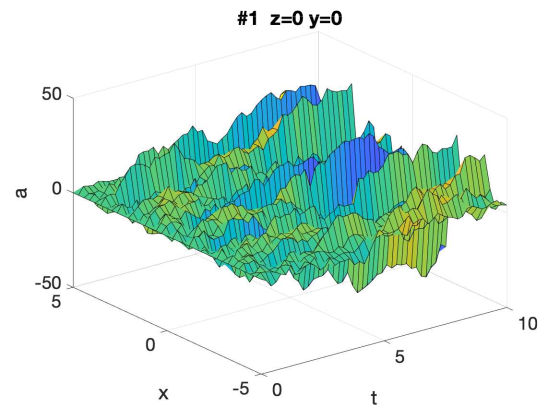
\includegraphics[width=0.75\textwidth]{Multi-Wiener}

\caption{\label{fig:The-simplest-case: Wiener-1}\emph{A multidimensional random
walk of a three-dimensional field projected onto $y=z=0$.}}
\vspace{10pt}
 
\end{figure}
\par\end{center}

For more interesting problems than this, more parameters are needed,
as explained next.

\section{SPDE parameters}

A stochastic partial differential equation or $SPDE$ for a complex
vector field is defined in both time $t$ and space dimension(s) $\mathbf{x}$.
The total \emph{dimensions} $d$ includes both time and space. To
solve a stochastic partial differential equation xSPDE involves a
similar procedure to the case of the SDE, covered in section \ref{sec:Simulating-an-SDE}.

The numerical solutions require additional parameters to define the
spatial grid, and to define the linear transformations in an interaction
picture, if spectral methods are used. The SPDE input parameters extend
those already introduced in (\ref{subsec:Simulation-parameters-1}).
Some new and extended parameters are listed in the table below: 
\begin{center}
\begin{tabular}{|c|c|c|c|}
\hline 
Label  & Type  & Typical value  & Description\tabularnewline
\hline 
\hline 
\emph{dimensions}  & integer  & $2$  & Space-time dimensions\tabularnewline
\hline 
\emph{linear\{c\}}  & function  & @(p) p.Dx  & Linear interaction picture function\tabularnewline
\hline 
\emph{ranges}  & real vector  & {[}10,10,...{]}  & Ranges in time and space\tabularnewline
\hline 
\emph{transforms\{c,d\}}  & integer vector  & $[1,0,1,..]$  & Space-time transform switch\tabularnewline
\hline 
\emph{points\{c\}}  & integer vector  & {[}51,35,..{]}  & Output lattice points in {[}t,x,y,z,..{]}\tabularnewline
\hline 
\textit{origins}  & real vector  & {[}0,-5,..{]}  & Space-time integration origin\tabularnewline
\hline 
\emph{boundaries\{c,d\}}  & integer array  & $[0,0;0,0]$  & Boundary type per field index\tabularnewline
\hline 
\emph{boundval\{c,d\}}  & array  & $[0,0;0,0]$  & Boundary value per field index\tabularnewline
\hline 
\emph{boundfun\{c,d\}}  & function  & {[}{]}  & Boundary function per field index\tabularnewline
\hline 
\end{tabular}
\par\end{center}

Setting $dimensions>1$ defines an (S)PDE as opposed to an ordinary
(S)DE. Here the cell index $i$ indicates a field index, and the cell
index $n$ gives the observable output or graph index.

In the xSPDE implementation, the total space-time \emph{dimensions}
is unlimited, although, large space-time dimensions become memory-intensive
and slow. There is a practical limit of about ten space-time dimensions
with current digital computers, unless you have a very large, fast
computer.

\subsection{SPDE spatial lattice}

Stochastic variables in an SPDE are stored in a real or complex array,
$a(i,\mathbf{\ell},e)$. Here $i$ is the internal field index, $\mathbf{\ell}$
is a $d-1$ dimensional spatial lattice index for \emph{d} space-time
dimensions, and $e$ is the ensemble index. To specify the spatial
lattice, one must define: 
\begin{description}
\item [{dimensions}] The dimensionality in time and space. The default
is an SDE: $d=1$. 
\item [{points}] The number of integration points. The default is $\mathbf{N}=[51,35,35..]$. 
\item [{ranges}] The integration ranges in each dimension. The default
is $\mathbf{R}=[10,10,10..]$. 
\item [{origins}] The origins of the space-time integration domains. By
default, the origin is $O\left(1\right)=0$ for the time coordinate
and $\mathbf{O}=-\mathbf{R}/2$ for the space coordinates ($\mathbf{R}$
is the $ranges$ variable) such that the spatial grid is symmetric
around $\mathbf{r}=0$. 
\end{description}

\subsection{Initial conditions}

Initial conditions are set at the initial time of $t=O_{1}$ with
a user-defined function so that: 
\begin{equation}
a(O_{1})=initial(v,p)
\end{equation}
The \emph{initial} function includes initial random fields $v=\left[v^{x},v^{k}\right]$.
Their correlations are either delta correlated or spatially correlated.
To allow this, the input parameter $randoms$ is a vector such that:
$randoms(1)$ is the number of delta-correlated random fields, $v^{x}$,
and $randoms(2)$ is the number of correlated random fields, $v^{k}$.
All random fields in the \emph{initial} function, even if correlated
using filters in momentum space, are transformed to position space
before use. If there is no filtering, $v^{x}$ and $v^{k}$ have the
same correlations.

\section{Next example}

As another very simple example, consider the SPDE

\begin{eqnarray}
\frac{\partial a}{\partial t} & = & -\frac{1}{4}a+x\cdot w\label{eq:simple_spde_example}
\end{eqnarray}

The system has one spatial dimension, or $d=2$ space-time dimensions,
one field and one noise variable. We suppose that the initial noise
variance is Gaussian, with: 
\begin{equation}
a(0,x)=10v(x).
\end{equation}
We want to consider $10,000$ stochastic trajectories per sub-ensemble
with$10$ sub-ensembles. We will set the origin for $x$ to $0$.
The variable $a$ will be initialized as delta-correlated in space
with a gaussian standard deviation on the lattice of $\sigma=10/\sqrt{\Delta V}$.
As our observable, we consider the second moment of $a$.

This is simulated through the following xSPDE code: 
\begin{center}
\doublebox{\begin{minipage}[t]{0.75\columnwidth}%
\texttt{clear;}

\texttt{p.name = 'simple SPDE';}

\texttt{p.dimensions = 2;}

\texttt{p.ensembles = {[}10000,10{]};}

\texttt{p.origins = {[}0,0{]};}

\texttt{p.noises = 1;}

\texttt{p.initial = @(v,p) 10{*}v;}

\texttt{p.observe = @(a,\textasciitilde ) a.\textasciicircum 2;}

\texttt{p.olabels = '\textless a\textasciicircum 2\textgreater
';}

\texttt{p.deriv = @(a,w,p) -0.25{*}a + p.x .{*} w;}

\texttt{xspde(p);}%
\end{minipage}} 
\par\end{center}

With this input, Matlab produces two output graphs:

\begin{figure}
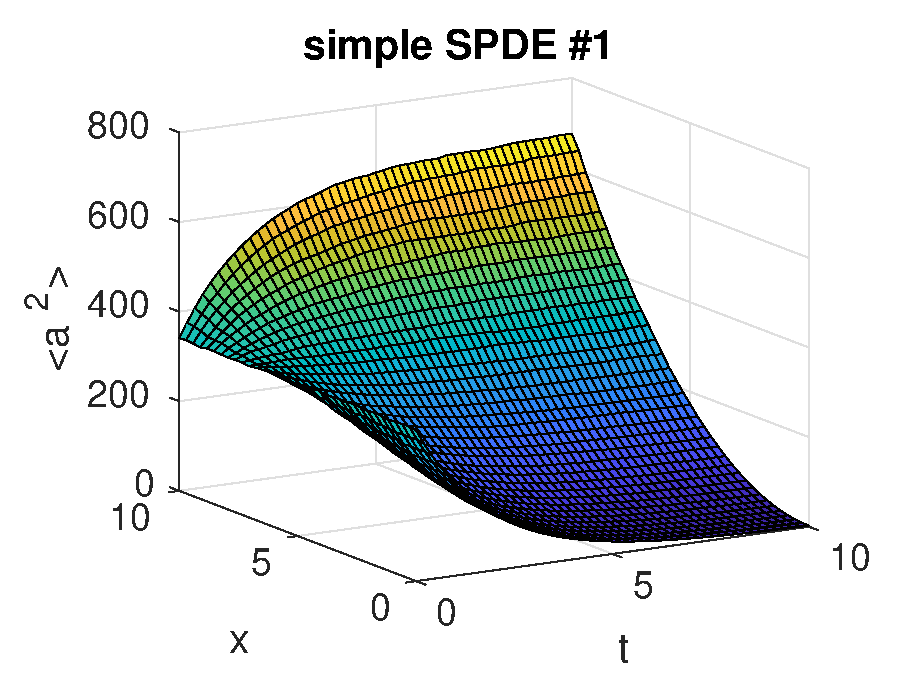
\includegraphics[width=0.5\textwidth]{simple_SPDE1}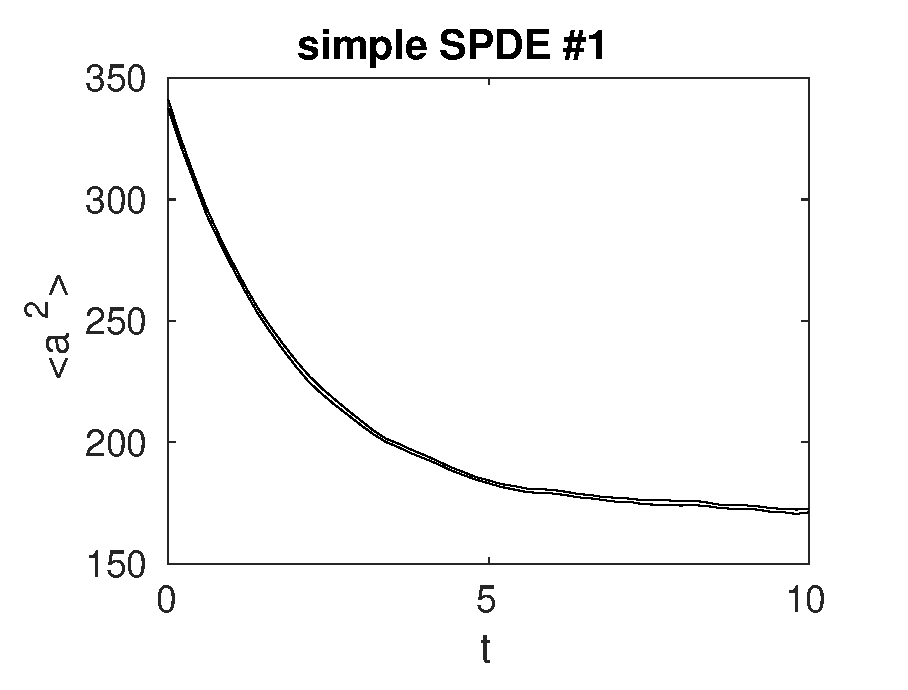
\includegraphics[width=0.5\textwidth]{simple_SPDE2}

\caption{\emph{Example: simple SPDE output graphs.}}
\vspace{10pt}
 
\end{figure}

The second graph shows the time evolution for $x$ at the mid-point,
$x=5$.\textbf{\textcolor{red}{{} }}The variances are larger than
they would be in the SDE case, where one might expect an initial variance
of $\left\langle a^{2}(0)\right\rangle =100$. The reason for this
is that the initial noise random and noise fields are replaced by
a lattice with a variance of $1/\Delta V$. In the default case, this
causes an increase in the local noise.

\section{Transverse lattice}

In the functions $deriv$, $initial$ and $observe$, the field and
noise variables $a$ and $w$ now have extended dimensionality compared
to the $1$-dimensional case, to index the transverse lattice. The
indices are $a\left(f,\mathbf{i},e\right)$, where the: 
\begin{description}
\item [{field}] index $f$ corresponds to the field index for $a$ and
the noise index for $w$. 
\item [{intermediate}] indices $\mathbf{i},$ which are absent in the $1$-dimensional
case, correspond to the spatial grid and have the same structure.
For example, in the case with \emph{dimensions = 3}, indicating one
time index and two spatial dimension, $\mathbf{i}$ corresponds to
the two space indices. 
\item [{last}] index $e$ corresponds to the stochastic trajectory. 
\end{description}
For storing space coordinates like $p.x$, the first and last index
are $f=e=1$. Where Fourier transforms are used internally, the momentum
arrays have zero momentum as the first index to follow standard discrete
Fourier transform conventions. This is changed to a symmetric convention
in all stored graphics data outputs.

As explained in section \ref{sec:IP-implementation}, the general
equation solved can be written in differential form as

\begin{equation}
\frac{\partial\mathbf{a}}{\partial t}=\mathbf{A}\left[\mathbf{a}\right]+\underline{\mathbf{B}}\left[\mathbf{a}\right]\cdot\mathbf{w}(t)+\underline{\mathbf{L}}\left[\mathbf{\nabla},\mathbf{a}\right]\,.
\end{equation}

The linear function $L$ can be input either inside the derivative
function using finite difference operators described below, or as
a separate \emph{linear} function, to allow for an interaction picture
in which case: 
\begin{equation}
\underline{\mathbf{L}}\left[\mathbf{\nabla},\mathbf{a}\right]=\,\underline{\mathbf{L}}\left[\mathbf{\nabla}\right]\mathbf{a}\,.
\end{equation}
This depends on momentum space coordinates, which involves Fourier
transforms and means that no space dependence is allowed. Spectral
methods in xSPDE are currently restricted to cases with linear derivative
terms and periodic or zero boundary conditions. It is also possible
to use finite differences, in which case the derivative terms are
included as part of the derivative function \emph{deriv}.

The usual FFT spectral methods require periodicity. The four other
boundary methods can currently only be used with the default boundary
values of zero, and with an interaction picture derivative that only
has even powers of derivatives. Additional spectral methods will be
included in a subsequent release: xSPDE4.

\subsection{Linear operator}

The field $x$ is provided by the parameter structure, and corresponds
to the variable $x$ in Eq \eqref{eq:simple_spde_example}. All parameters
are preceded by the parameter structure label. Likewise, for higher
dimensional problems, the variables $y$ and $z$ exist. These are
placeholders for $r\{1\},r\{2\},r\{3\}$, so the spatial variables
of even higher dimensional problems can be accessed through $r\{n\}$.

Using a linear operator in an SPDE gives better accuracy, and allows
use of the interaction picture. This is included automatically for
all built-in xSPDE algorithms, provided the \emph{linear} function
is defined in the parameter structure. Variables $p.D\{i\}$ (with
placeholders $p.Dx,p.Dy,p.Dz$ for the first 3 spatial dimensions)
provide access to the derivative operator. Higher-order derivatives
are found through potentiating $p.Dx$ accordingly.

For example, the $2$-dimensional Laplacian operator 
\begin{equation}
\nabla^{2}=\frac{\partial^{2}}{\partial x^{2}}+\frac{\partial^{2}}{\partial y^{2}}
\end{equation}
corresponds to a linear differential operator specified as: 
\begin{equation}
p.linear=@(p)\,\,\,p.Dx.^{2}+p.Dy^{2};
\end{equation}
For a comprehensive list of variables accessible through the $p$-structure,
refer to sec. \ref{sec:Table-of-parameters}.

\subsection{Integrals and averages}

\label{xsim:averages} There are functions available in xSPDE for
spatial grid averages and integrals, to handle the spatial grid. These
are \textbf{\emph{Ave}}\emph{ }and\emph{ }\textbf{\emph{Int,}} which
are used to calculate observables for plotting. They operate in parallel
over the lattice dimensions, by taking a vector or scalar quantity,
for example a single field component, and returning an average or
a space integral. In each case the first argument is the field, the
second argument is a vector defining the type of operation, and the
last argument is the parameter structure. If there are two arguments,
the operation vector is replaced by its default value.

Integrals over the spatial grid allow calculation of global quantities.
To take an integral over the spatial grid, use the xSPDE function
\emph{Int} with arguments \emph{(o, {[}dx, {]} p)}.

This function takes a scalar or vector quantity \emph{o}, and returns
a trapezoidal space integral over selected dimensions with vector
measure \emph{dx}. If\emph{ $dx(j)>0$} an integral is taken over
dimension \emph{j}. Dimensions are labelled from \emph{j = 1,2,3 ...}
as in all xSPDE standards. Time integrals are ignored at present.
Integrals are returned at all lattice locations. To integrate over
an entire lattice, set \emph{dx = p.dx}, otherwise set \emph{dx(j)
= p.dx(j)} for selected dimensions \emph{j}.

If momentum-space integrals are needed, first use the \emph{transforms}
switch to make sure that the field is Fourier transformed before being
averaged, and input \emph{dk} instead of \emph{dx}.

Spatial grid averages can be used to obtain stochastic results with
reduced sampling errors if the overall grid is homogeneous. An average
is carried out using the builtin xSPDE function \emph{Ave()} with
arguments \emph{(o, {[}av, {]} p)}.

This takes a vector or scalar field or observable, defined on the
lattice, and returns an average over the spatial lattice. The input
is a field \emph{a} or observable \emph{o}, and an optional averaging
switch \emph{av}. If $av(j)>0$, an average is taken over dimension
\emph{j}. Space dimensions are labelled from \emph{j = 2,3...} as
elsewhere. If the \emph{av} vector is omitted, the average is taken
over all space directions.

\subsection{One space-dimensional example}

A famous partial differential equation is an exactly soluble equation
for a soliton, the nonlinear Schrödinger equation (NLSE): 
\begin{equation}
\frac{da}{dt}=\frac{i}{2}\left[\nabla^{2}a-a\right]+ia\left|a\right|^{2}.
\end{equation}

Together with the initial condition that $a(0,x)=sech(x)$, this has
a soliton, an exact solution that doesn't change in time: 
\begin{eqnarray}
a(t,x) & = & sech(x).
\end{eqnarray}
The spatial integral is simply: 
\begin{eqnarray}
\int sech(x)dx & = & \pi.
\end{eqnarray}

An xSPDE code that solves this is given below, together with code
that compares the numerical solution with the exact solutions for
the soliton and the integral: 
\begin{center}
\doublebox{\begin{minipage}[t]{0.75\columnwidth}%
\texttt{p.name = 'NLS soliton';}

\texttt{p.dimensions = 2;}

\texttt{p.initial = @(v,p) sech(p.x);}

\texttt{p.deriv = @(a,\textasciitilde ,p) 1i{*}a.{*}(conj(a).{*}a);}

\texttt{p.linear = @(p) 0.5{*}1i{*}(p.Dx.\textasciicircum 2-1.0);}

\texttt{p.olabels = \{'a(x)','\textbackslash int a(x) dx'\};}

\texttt{p.observe\{2\} = @(a,p) Int(a, p);}

\texttt{p.compare\{1\} = @(p) sech(p.x);}

\texttt{p.compare\{2\} = @(p) pi;}

\texttt{e = xspde(p);}%
\end{minipage}} 
\par\end{center}

Due to finite boundaries and discrete spatial lattice, the agreement
is not perfect. The errors can be reduced by increasing the range
of the integration domain and improving the resolution with more points.

\subsection{Two space-dimensional example}

As another example, consider the two-dimensional nonlinear stochastic
equation, with periodic boundary conditions:

\begin{eqnarray}
\frac{\partial a}{\partial t} & = & \nabla^{2}a\left(\mathbf{x},t\right)+a\left(\mathbf{x},t\right)-a\left(\mathbf{x},t\right)^{3}+\eta\left(\mathbf{x},t\right).\label{eq:Nonlinear-SPDE-example}
\end{eqnarray}

Using the interaction picture allows for the absorption of both the
Laplacian and the first-order term by the \textit{p.linear} parameter,
which results in 
\begin{center}
\doublebox{\begin{minipage}[t]{0.75\columnwidth}%
\texttt{...}

\texttt{p.linear = @(p) (p.Dx.\textasciicircum 2+p.Dy.\textasciicircum 2)
+ 1;}

\texttt{p.deriv = @(a,w,\textasciitilde ) -a.\textasciicircum 3
+ w;}

\texttt{xspde(p);}%
\end{minipage}} 
\par\end{center}

With this input, Matlab produces two output graphs:

\begin{figure}
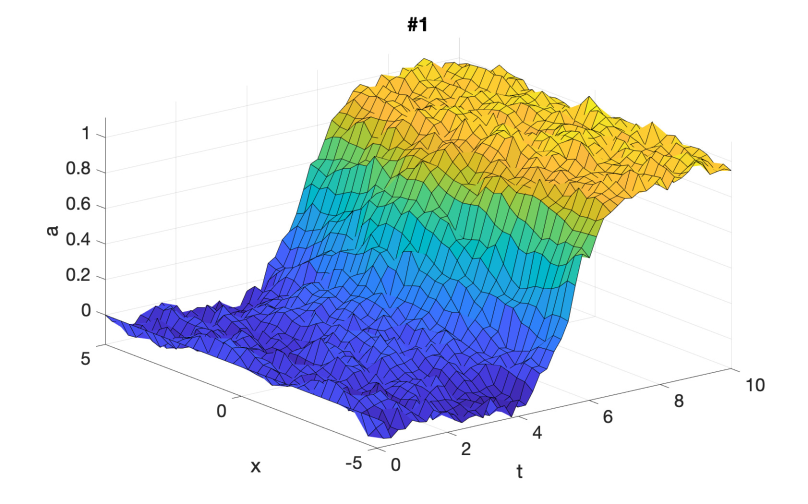
\includegraphics[width=0.5\textwidth]{TwoD-example}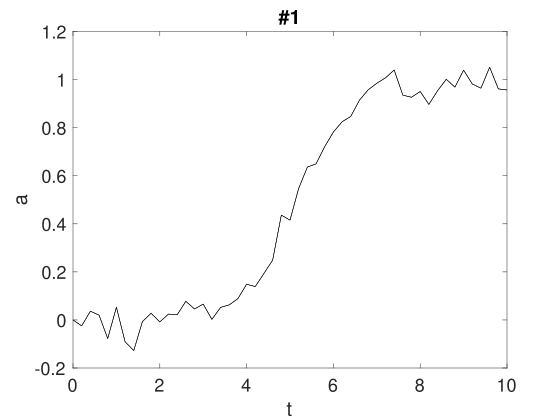
\includegraphics[width=0.5\textwidth]{TwoD-example1}

\caption{\emph{Two space-dimensional example graphs.}}
\vspace{10pt}
 
\end{figure}


\section{Finite differences }

Instead of using the interaction picture, xSPDE also has finite difference
methods for direct differentiation. These derivatives are obtained
through function calls $D1$ and $D2$ respectively for first and
second derivatives, which use a fixed grid spacing. As elsewhere,
they can be replaced by user-written functions if preferred. Generally
they require smaller steps in time than spectral methods, when used
to define the derivative.

\subsection{Finite difference first derivatives}

The code to take a first order spatial derivative with finite difference
methods is carried out using the xSPDE function\emph{ D1()} with arguments
\emph{(o, {[}dir, {]} p)}.

This takes a scalar or vector \emph{o} and returns a first derivative
in an axis direction \emph{dir}. Set \emph{dir = 2} for an x-derivative,
\emph{dir = 3} for a y-derivative, and so on. Time derivatives are
ignored at present. Derivatives are returned at all lattice locations.

If the direction is omitted, an \emph{x}-derivative is returned. These
derivatives can be used both in calculating propagation and in calculating
observables. The boundary condition is set by the \emph{boundaries}
input. It can be made periodic, which is the default, or Neumann with
zero derivative, or Dirichlet with zero field.

\subsection{Finite difference second derivatives}

The code to take a second order spatial derivative with finite difference
methods is carried out using the xSPDE \emph{D2} function with arguments
\emph{(o, {[}dir, {]} p)}.

This takes a scalar or vector \emph{o} and returns the second derivative
in axis direction \emph{dir}. Set \emph{dir = 2} for an x-derivative,
\emph{dir = 3} for a y-derivative and so on. All other properties
are exactly the same as \emph{D1}.

Without using the interaction picture, the stochastic equation of
Eq \eqref{eq:Nonlinear-SPDE-example} is specified in xSPDE using
finite differences as 
\begin{center}
\doublebox{\begin{minipage}[t]{0.75\columnwidth}%
\texttt{p.dimensions = 3;}

\texttt{p.steps = 50;}

\texttt{p.deriv = @(a,w,p) D2(a,2,p)+D2(a,3,p)+a - a.\textasciicircum 3
+...}

\texttt{w/10;}

\texttt{xspde(p);}%
\end{minipage}} 
\par\end{center}

This gives the same result as with the linear propagator, although
requiring smaller step-sizes for numerical stability, with an output
graph shown in Fig (\ref{fig:Two-space-dimensional-example-direct-diff}).
Note that the parameters and noises are slightly different!

\begin{figure}
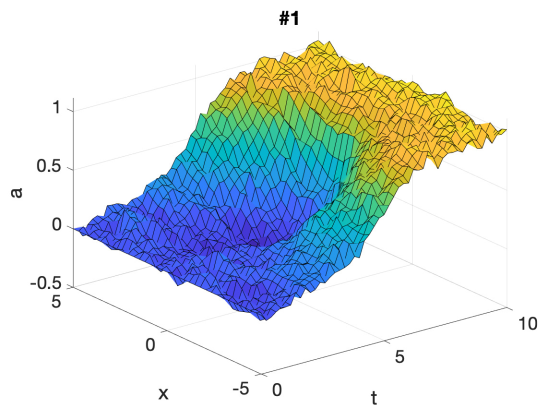
\includegraphics[width=0.5\textwidth]{TwoD-example-direct}\includegraphics[width=0.5\textwidth]{TwoD-example-direct1}

\caption{\emph{Two space-dimensional example graphs, direct differentiation}.\label{fig:Two-space-dimensional-example-direct-diff}}
\vspace{10pt}
 
\end{figure}


\section{Boundary conditions}

\subsection{Transverse boundaries}

Transverse boundary conditions must be given for all partial differential
equations. Common transverse \emph{boundary types} are of three types:
Neumann (specified derivative), periodic, or Dirichlet (specified
field). These are obtained using $boundaries\{d\}=-1,0,1$, which
is specified for each space dimension $d>1$, field index and boundary.

If \emph{boundaries} are omitted for any dimension the default is
$0$, which gives periodic boundaries in that dimension for all field
indices, and permits the use of Fourier transforms and an interaction
picture as described above.

The value of $boundaries\{d\}$ is a matrix whose column index $(i)$
is the field index, and whose row index (j) is given by $j=1,2$ for
the lower and upper boundary type respectively.

Spatial derivatives or other functions linking different spatial points
can be specified either in the functionals $\boldsymbol{A}\left[\mathbf{a},\mathbf{r}\right]$,
$\underline{\mathbf{B}}\left[\mathbf{a},\mathbf{r}\right]$ or else
in the $linear$ function, provided the derivative terms are linear
functions of the fields. Use of the $linear$ function allows an interaction
picture algorithm, with increased efficiency. The $linear$ function
is currently only available with periodic boundary conditions.

The default boundary conditions are periodic. The implicit setting
of this is that periodicity is enforced such that $a\left(o_{i}-dx_{i}/2\right)=a\left(o_{i}+r_{i}+dx_{i}/2\right)$
, which is the usual discrete Fourier transform requirement.

Otherwise, the differential equation boundaries are specified at $a\left(o_{i}\right)$,
$a\left(o_{i}+r_{i}\right)$, using the cell-array input $boundaries\{d\}(i,j)$,
which is defined per space dimension ($d=2,3..$), field index ($i=1,2..$)
and boundary $j=(1,2)$. Here $d>1$ is the transverse dimension,
not including time, which only has an initial condition.

In summary the available boundary types are: 
\begin{description}
\item [{Neumann:}] For specified \emph{derivative} boundaries, $boundaries\{d\}(i,j)=-1$ 
\item [{Periodic:}] For \emph{periodic} boundaries, $boundaries\{d\}(i,j)=0$ 
\item [{Dirichlet:}] For specified \emph{field} boundaries, $boundaries\{d\}(i,j)=1$ 
\end{description}
These are specified in a cell array: $boundaries\{d\}(i,1)$ sets
the lower boundary type in dimension \emph{d}, for the \emph{i -th
}field component\emph{ }while $boundaries\{d\}(i,2)$ gives the upper
boundary type. Each space dimension, variable and boundary is set
independently. In xSPDE, the equations are always initial value problems
in time, so the time dimension boundary specification for $d=1$ is
not included.

\paragraph{Example: boundary types in a 2-dimensional PDE}

Suppose there are two fields, and we wish to set mixed boundaries
in space, with Dirichlet in the past and Neumann in the future for
the first field $a(1,:)$, with the opposite combination in the second
field component, $a(2,:)$: 
\begin{center}
\doublebox{\begin{minipage}[t]{0.75\columnwidth}%
\texttt{p.boundaries\{2\} = {[}1,-1;-1,1{]};}%
\end{minipage}} 
\par\end{center}

Note that the field cell index is $c=1$, which can be omitted.

\subsection{Transverse boundary values}

For non-vanishing, specified boundary conditions, the boundary value
can be entered using $boundval(a,p)$, or else, if it is dynamical,
the function $boundfun(a,p)$ is called. This returns the boundary
values used for the fields or derivatives in a particular dimension
$d>1$ as an array of dimension $b(\mathbf{j},e))$, where $\mathbf{j}=i,\mathbf{k}$.

Here $i=j_{1}$ is the field index, and $\mathbf{k}$ is the space
index, where $j_{d}$ is the index of the dimension whose boundary
values are specified. For this dimension, only two values are needed:
$j_{d}=1,2$ for the lower and upper boundary values, which could
either be field values or their derivatives. An ensemble index $e$
is also needed if the boundary values are stochastic.

Boundary values can be a function of both the fields ($a$) and internal
variables like the current time ($t$). These may have stochastic
initial values at $t=0$ which are calculated only once. In such cases
the boundary values must first be initialized, so the routine $boundfun(a,p)$
is first internally initialized with time $t<origin(1)$, and with
random Gaussian values in the input field $a$. These are delta-correlated
in space, i.e., with the same definition as ``inrandoms''. The xSDPE
program stores the returned values $b$ for the boundaries in an internal
cell array, $boundval\{c,d\}$, for later use if required.

The default boundary value is zero, if not specified.

\textbf{NOTE: Current xSPDE code requires finite-difference methods
to be used with $boundfun$. Spectral methods use the default boundary
conditions. }

\subsection{Example: boundaries in a 2-dimensional PDE}

Suppose there are two fields, and we wish to set boundary values.

We take boundary values as Dirichlet for $x=0$ and Neumann for $x=1$
in field variable 1, and Neumann for $x=0$ and Dirichlet for $x=1$
in field variable 2, that are different from the default values of
$a=0$, $\partial_{x}a=0$, so that: 
\begin{align}
a_{1}\left(x=0\right) & =1,\nonumber \\
\partial_{x}a_{1}\left(x=1\right) & =a_{1}\left(x=1\right).\nonumber \\
\partial_{x}a_{2}\left(x=0\right) & =-a_{2}\left(x=0\right)\nonumber \\
a_{2}\left(x=1\right) & =-1.
\end{align}

These are set in the following code: 
\begin{center}
\doublebox{\begin{minipage}[t]{0.75\columnwidth}%
\texttt{p.boundfun\{1,2\} = @mybfun}

\texttt{p.boundaries\{2\} = {[}1,-1;-1,1{]};}

\texttt{...}

\texttt{function b = mybfun(a,p)}

\texttt{\% b = mybfun(a,p) calculates boundary values}

\texttt{b(1,2,:) = a(1,end,:);}

\texttt{b(2,1,:) = -a(2,end,:);}

\texttt{b(1,1,:) = 1;}

\texttt{b(2,2,:) = -1;}

\texttt{end}%
\end{minipage}} 
\par\end{center}

\subsection{Transverse plots}

A number of plots at equally spaced points in time can be generated
through. For example, adding the line below creates 3 time-sliced
plots at $t=0,5,10$: 
\begin{center}
\doublebox{\begin{minipage}[t]{0.75\columnwidth}%
\texttt{p.transverse\{1\} = 3;}%
\end{minipage}} 
\par\end{center}

\section{Output transforms}

For graphical output, Fourier transforms involve a sum over the lattice
points using a discrete Fourier transform at the lattice points $x_{i}$,
so that:

\begin{equation}
\tilde{a}(\omega_{i},\mathbf{k}_{i})=\frac{dtd\mathbf{x}}{\left[2\pi\right]^{d/2}}\sum_{j_{1}\ldots j_{d}}\exp\left[i\left(\omega_{i_{1}}t_{j_{1}}-\mathbf{k}_{\mathbf{i}}\cdot\mathbf{x}_{\mathbf{j}}\right)\right]a(t_{j_{1}},\mathbf{x}_{\mathbf{j}})\,
\end{equation}
The momenta $k_{i}$ have an interval of 
\begin{equation}
dk_{i}=\frac{2\pi}{n_{i}dx_{i}}
\end{equation}
with $k_{i}$ values given for even n by: 
\begin{equation}
k_{i}=\left(1-\frac{n_{i}}{2}\right)dk_{i},\ldots\frac{n_{i}}{2}dk_{i}
\end{equation}
and for odd n by: 
\begin{equation}
k_{i}=\frac{1-n_{i}}{2}dk_{i},\ldots\frac{n_{i}-1}{2}dk_{i}
\end{equation}

Once Fourier transformed, the $observe$ function can be used to take
any further functions or combinations of Fourier transformed fields
prior to averaging. Important points to keep in mind are as follows: 
\begin{itemize}
\item Fourier transforms are specified for the k-th \emph{observe }function
independently of all other functions, by specifying $transforms\{k\}=\left[\ell_{1,}\ldots\ell_{d,}\right]$. 
\item Here $\ell_{j}=0,1$ is a logical switch, set to to $\ell_{j}=1$
if the $j-th$ dimension requires a Fourier transform, and $\ell_{j}=0$
if there is no Fourier transform. 
\item The internal fields $p.k\{1\},\ldots p.k\{d\}$ are available for
use in making functions of momentum for use with observations. 
\item In propagation calculations, the momentum lattice values start with
$k=0,\ldots$, following standard Matlab and FFT conventions. 
\item For storing and graphing, momentum lattice values are reordered to
start with $k=-k_{max},\ldots$, following standard graphics and mathematical
conventions. 
\end{itemize}

\section{Initial random fields}

Fourier transforms are available for use both on initial random values
and on noise fields during time-evolution. This is controlled by the
second element of $randoms$ and $noises$, respectively.

When $randoms(1)>0$, an initial random field $\mathbf{v}^{x}$ is
generated with delta-correlations in $x$-space. When $randoms(2)>0$,
an initial random field $\tilde{\mathbf{v}}^{k}$ is generated with
delta-correlations in $k$-space. This can be filtered with a user-specified
filter function to give $\tilde{\mathbf{v}}^{kf}$, then inverse Fourier
transformed to give $v^{k}$. Both random fields are passed to the
$initial$ function as an extended vector $\left[v^{x},v^{k}\right]$,
for field \emph{initialization} in space.

There is a user specified filter function available, to modify random
fields $\tilde{v}^{k}$, that are delta-correlated in momentum space
using a filter function, '\emph{rfilter}' so that $v_{i}^{kf}\left(\mathbf{k}\right)=f_{i}^{(r)}\left(\mathbf{v}^{k}\left(\mathbf{k}\right)\right)$,
before being used. The corresponding correlations are: 
\begin{eqnarray}
\left\langle v_{i}^{x}\left(\mathbf{x}\right)v_{j}^{x}\left(\mathbf{x}'\right)\right\rangle  & = & \delta\left(\mathbf{x}-\mathbf{x}'\right)\delta_{ij}\sim\frac{1}{\Delta V}\delta_{\mathbf{x},\mathbf{x}'}\delta_{ij}\nonumber \\
\left\langle \tilde{v}_{i}^{k}\left(\mathbf{k}\right)\tilde{v}_{j}^{k}\left(\mathbf{k}'\right)\right\rangle  & = & \delta\left(\mathbf{k}-\mathbf{k}'\right)\delta_{ij}\sim\frac{1}{\Delta K}\delta_{\mathbf{k},\mathbf{k}'}\delta_{ij}\nonumber \\
\left\langle \tilde{v}_{i}^{kf}\left(\mathbf{k}\right)\tilde{v}_{j}^{kf}\left(\mathbf{k}'\right)\right\rangle  & = & \left\langle f_{i}^{(r)}\left(\tilde{\mathbf{v}}^{k}\left(\mathbf{k}\right)\right)f_{j}^{(r)}\left(\tilde{\mathbf{v}}^{k}\left(\mathbf{k}'\right)\right)\right\rangle .
\end{eqnarray}

Note that on a lattice, we replace the Dirac continuous delta-function
by a discrete Kronecker delta function scaled by an inverse volume
element either in space ($\Delta V$) or momentum ($\Delta K$) .
The xSPDE Fourier transforms are given by a symmetric Fourier transform,
so that if we inverse Fourier-transform the $k-$space \emph{inrandoms},
without filtering, then: 
\begin{equation}
v^{k}(\mathbf{x})=\frac{1}{\left[2\pi\right]^{(d-1)/2}}\int e^{i\mathbf{k}\cdot\mathbf{x}}\tilde{v}^{k}(\mathbf{k})d\mathbf{k}\,
\end{equation}

These have random initial values that are real and delta-correlated
in space, so that: 
\begin{equation}
\left\langle v^{x}\left(\mathbf{x}\right)v^{x}\left(\mathbf{x}'\right)\right\rangle =\delta\left(\mathbf{x}-\mathbf{x}'\right).
\end{equation}
The corresponding noises in position space are correlated according
to:

\begin{align}
\left\langle v^{k}\left(\mathbf{x}\right)\left(v^{k}\left(\mathbf{x}'\right)\right)^{*}\right\rangle  & =\frac{1}{\left[2\pi\right]^{(d-1)}}\int e^{i(\mathbf{k}\cdot\mathbf{x}-\mathbf{k}'\cdot\mathbf{x}')}\left\langle \tilde{v}^{k}\left(\mathbf{k}\right)\tilde{v}^{k}\left(\mathbf{k}'\right)\right\rangle d\mathbf{k}d\mathbf{k}'\nonumber \\
 & =\frac{1}{\left[2\pi\right]^{(d-1)}}\int e^{i(\mathbf{x}-\mathbf{x}')\cdot\mathbf{k}}d\mathbf{k}\nonumber \\
 & =\delta\left(\mathbf{x}-\mathbf{x}'\right).
\end{align}
Similarly, if we don't conjugate the k-noise, then: 
\begin{equation}
\left\langle v^{k}\left(\mathbf{x}\right)v^{k}\left(\mathbf{x}'\right)\right\rangle =\delta\left(\mathbf{x}+\mathbf{x}'\right).
\end{equation}

However, if we define $\tilde{v}^{c}\left(\mathbf{k}\right)=\left[\tilde{v}_{1}^{k}\left(\mathbf{k}\right)+i\tilde{v}_{2}^{k}\left(\mathbf{k}\right)\right]/\sqrt{2}$
, then we obtain complex noise that is only delta correlated when
conjugated. 
\begin{align}
\left\langle v^{c}\left(\mathbf{x}\right)\left(v^{c}\left(\mathbf{x}'\right)\right)^{*}\right\rangle  & =\delta\left(\mathbf{x}-\mathbf{x}'\right)\nonumber \\
\left\langle v^{c}\left(\mathbf{x}\right)v^{c}\left(\mathbf{x}'\right)\right\rangle  & =0.
\end{align}
This is obtainable with the x-space noise as well, but the utility
of the k-space noise is that it can be filtered to have nonlocal correlations
in space if required.

During propagation in time, $\mathbf{w}=\left[\mathbf{w}^{x},\mathbf{w}^{k}\right]$
are real noise fields that are delta-correlated in space-time. They
are calculated in an analogies way, except with an additional factor
of $1/\sqrt{dt}$ because they are delta correlated in time as well.There
is a user specified scaling function available, to take random noises
$w^{k}$ in momentum space that are then scaled using a filter function,
'\emph{nfilter}' so that $w_{i}^{kf}\left(\mathbf{k}\right)=f_{i}^{(n)}\left(\mathbf{w}^{k}\left(\mathbf{k}\right)\right)$,
before being used:

\begin{eqnarray}
\left\langle w_{i}^{x}\left(t,\mathbf{x}\right)w_{j}^{x}\left(t,\mathbf{x}'\right)\right\rangle  & = & \delta\left(\mathbf{x}-\mathbf{x}'\right)\delta\left(t-t'\right)\delta_{ij}\nonumber \\
\left\langle \tilde{w}_{i}^{k}\left(t,\mathbf{k}\right)\tilde{w}_{j}^{k}\left(t,\mathbf{k}'\right)\right\rangle  & = & \delta\left(\mathbf{k}-\mathbf{k}'\right)\delta\left(t-t'\right)\delta_{ij}\nonumber \\
\left\langle \tilde{w}_{i}^{kf}\left(t,\mathbf{k}\right)\tilde{w}_{j}^{kf}\left(t',\mathbf{k}'\right)\right\rangle  & = & \left\langle f_{i}^{(n)}\left(\tilde{\mathbf{w}}^{k}\left(t,\mathbf{k}\right)\right)f_{j}^{(n)}\left(\tilde{\mathbf{w}}^{k}\left(t',\mathbf{k}'\right)\right)\right\rangle .
\end{eqnarray}


\section{Scanned parameter plots}

Since xSIM is a function that can be called, plots of results against
simulation parameters are possible. This requires repeated calls to
xSIM with different parameter values, together with data storage in
an xGRAPH compatible form, and a call to xGRAPH. If different random
seeds are required, the seed needs to be reset in each call. The relevant
axes points plotted, labels and the values of scanned parameters also
need to be input.

The simulation function xSIM uses the last data array index, $c$,
to store the data values and up to two corresponding errors. This
takes up three index values. A value of $c=4$ is used to store comparison
data, and its errors if there are any in $c=5,6$. This can be used
for exact results, approximations, or experimental data.

\begin{figure}
\centering{}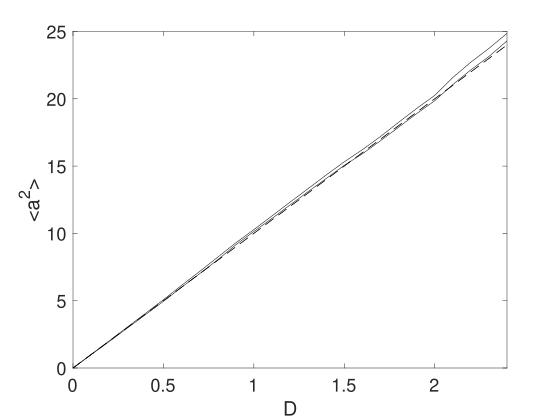
\includegraphics[width=0.75\textwidth]{Scan}

\caption{\label{fig:Scanned-diffusion}\emph{Scanned parameter output with
a variable diffusion, for the case of a pure Wiener process, $\dot{a}=Bw(t)$.
Exact value is the dashed line.}}
\vspace{10pt}
 
\end{figure}


\subsection{Example: Scanned diffusion}

As an example, consider the simplest possible stochastic equation,
with a scanned diffusion: 
\begin{equation}
\dot{a}=Bw(t)\,.
\end{equation}

The equation is integrated over the interval $t=0:10$, with $a=0$
initially, using $10^{4}$ trajectories to give an expected error
of around $\pm1\%$. The variance of $a$ at $t=10$ is plotted as
a function of $D=B^{2}$, then compared to an exact value. The result
is in Fig (\ref{fig:Scanned-diffusion}). The corresponding code is
given as well. 
\begin{center}
\doublebox{\begin{minipage}[t]{0.75\columnwidth}%
\texttt{function e = WienerScan()}

\texttt{p.name = 'Wiener process';}

\texttt{p.ensembles = {[}1000,10{]};}

\texttt{p.points = 12;}

\texttt{p.deriv = @(a,z,p) z{*}p.B;}

\texttt{p.observe = @(a,p) a.\textasciicircum 2;}

\texttt{p.olabels = \{'\textless a\textasciicircum 2\textgreater
'\};}

\texttt{p.glabels\{1\} = \{'D'\};}

\texttt{scanpoints = 25;}

\texttt{data\{1\}\{1\} = zeros(1,scanpoints,4);}

\texttt{for j = 1:scanpoints}

\texttt{\quad{}p.seed = j;}

\texttt{\quad{}p.B = sqrt((j-1){*}0.1);}

\texttt{\quad{}{[}e,data1,input,\textasciitilde{]} = xsim(p);}

\texttt{\quad{}data\{1\}\{1\}(1,j,1:3) = data1\{1\}\{1\}(1,p.points,:);}

\texttt{\quad{}xk\{1\}\{1\}(j) = p.B\textasciicircum 2;}

\texttt{\quad{}D(j) = p.B\textasciicircum 2;}

\texttt{end}

\texttt{data\{1\}\{1\}(1,:,4) = input.ranges(1){*}D(:);}

\texttt{input.xk = xk;}

\texttt{input.axes\{1\}\{1\} = 1:scanpoints;}

\texttt{xgraph(data,input);}

\texttt{end}%
\end{minipage}} 
\par\end{center}

Here $p.deriv$ defines the time derivative function $\dot{a}$, with
$w$ being the delta-correlated Gaussian noise that is generated internally.

\section{Project examples}

\subsection{Kubo project}

To get started on more complex programs, we next simulate the Kubo
oscillator, which is an oscillator with a random frequency: 
\begin{equation}
\dot{a}=iaw.
\end{equation}


\subsection*{Exercises}
\begin{itemize}
\item Simulate the Kubo oscillator using a file, $Kubo.m$, with two ensemble
levels to allow sampling error estimates. The error vector $error$
gives the total time-step error plus the sampling error. 
\item Increase the first ensemble size to check how it modifies the sampling
errors. 
\end{itemize}
\begin{center}
\doublebox{\begin{minipage}[t]{0.75\columnwidth}%
\texttt{function {[}error{]} = Kubo()}

\texttt{p.name = 'Kubo oscillator';}

\texttt{p.ensembles = {[}400,16{]};}

\texttt{p.initial = @(v,p) 1;}

\texttt{p.deriv = @(a,w,\textasciitilde ) 1i{*}a.{*}w;}

\texttt{p.olabels = \{'\textless a\_1\textgreater '\};}

\texttt{p.file = 'kubo.mat';}

\texttt{{[}error,\textasciitilde ,\textasciitilde ,\textasciitilde{]}
= xsim(p);}

\texttt{xgraph(p.file);}

\texttt{end}%
\end{minipage}} 
\par\end{center}

This function generates a data file, \texttt{kubo.mat}. If you run
this twice without deleting the earlier file, you will get a warning
and the old file will be moved to a backup file-name, \texttt{kubo\_1.mat},
to protect the earlier data. Note that xGRAPH will graph the data
in the most recent file saved.

You can also include modified graphics parameters as a second input
when running \texttt{xGRAPH, }just in case the first graphs you generate
need further changes.

\subsection{Gaussian diffraction}

Free diffraction and absorption of a Gaussian wave-function in $d-1=s$
space dimensions, is given by the partial differential equation (PDE):
\begin{equation}
\frac{da}{dt}=-\frac{\gamma}{2}a+\frac{i}{2}D\nabla^{2}a.
\end{equation}

The corresponding stochastic partial differential equation (SPDE)
includes additional noise, so that:

\begin{equation}
\frac{da}{dt}=-\frac{\gamma}{2}a+\frac{i}{2}D\nabla^{2}a+bw(t,x).
\end{equation}

The xSPDE spectral definition in space is: 
\begin{equation}
\tilde{a}(t,\mathbf{k})=\frac{1}{\left[2\pi\right]^{s/2}}\int e^{i\mathbf{k}\cdot\mathbf{x}}a(t,\mathbf{x})d\mathbf{x}\,.
\end{equation}

Together with the initial condition that $a(0,x)=exp(-\left|\mathbf{x}\right|^{2}/2)$,
this has an exact solution for the diffracted intensity with $b=0$,
in either ordinary space or momentum space: 
\begin{eqnarray}
\left|a\left(t,\mathbf{x}\right)\right|^{2} & = & \frac{1}{\left(1+\left(Dt\right)^{2}\right)^{s/2}}exp\left(-\left|\mathbf{x}\right|^{2}/\left(1+\left(Dt\right)^{2}\right)-\gamma t\right)\nonumber \\
\left|\tilde{a}\left(t,\mathbf{k}\right)\right|^{2} & = & exp\left(-\left|\mathbf{k}\right|^{2}-\gamma t\right).
\end{eqnarray}


\subsection*{Exercises}
\begin{itemize}
\item Simulate Gaussian diffraction in three dimensions using an xSPDE function 
\item Check your results against the exact solution 
\item The example below stores data in a standard HDF5 file. 
\end{itemize}
\begin{center}
\doublebox{\begin{minipage}[t]{0.75\columnwidth}%
\texttt{function {[}e{]} = Gaussian()}

\texttt{p.dimensions = 4;}

\texttt{p.initial = @(v,p) exp(-0.5{*}(p.x.\textasciicircum 2+p.y.\textasciicircum 2+p.z.\textasciicircum 2));}

\texttt{p.linear = @(p) 1i{*}0.05{*}(p.Dx.\textasciicircum 2+p.Dy.\textasciicircum 2+p.Dz.\textasciicircum 2);}

\texttt{p.observe = @(a,p) a.{*}conj(a);}

\texttt{p.olabels = '\textbar a(x)\textbar\textasciicircum 2';}

\texttt{p.file = 'Gaussian.h5';}

\texttt{p.images = 4;}

\texttt{e = xsim(p);}

\texttt{xgraph(p.file);}

\texttt{end}%
\end{minipage}} 
\par\end{center}
\begin{itemize}
\item \textbf{Add an additive complex noise of $0.01(w_{1}+iw_{2}$) to
the Gaussian differential equation, then replot with an average over
$100$ samples.} 
\item Work out the exact solution and repeat the comparisons. 
\end{itemize}
Note that for this, you'll need to add: $p.deriv=@(a,w,p)\,\,..+0.01*(w(1,:)+i*w(2,:))$

\section{Examples}

\subsection{Stochastic Ginzburg-Landau}

Including two space dimensions, or space-time dimensions of $d=3$,
an example of a SPDE is the stochastic Ginzburg-Landau equation. This
describes symmetry breaking. The system develops a spontaneous phase
which varies spatially as well. The model is used to describe lasers,
magnetism, superconductivity, superfluidity and particle physics:
\begin{equation}
\dot{a}=\left(1-\left|a\right|^{2}\right)a+bw(t)+c\nabla^{2}a
\end{equation}
where 
\begin{equation}
\left\langle w(x)w^{*}(x')\right\rangle =2\delta\left(t-t'\right)\delta\left(x-x'\right).
\end{equation}

The following new ideas are introduced for this problem: 
\begin{enumerate}
\item \textbf{$\mathtt{dimensions}$ is the space-time dimension.} 
\item \textbf{The} 'dot' \textbf{notation used for parallel operations over
lattices}. 
\item \textbf{$\mathtt{linear}$ is the linear operator - a Laplacian in
these cases.} 
\item \textbf{$\mathtt{images}$ produces movie-style images at discrete
time slices.} 
\item \textbf{$\mathtt{Dx}$ indicates a derivative operation, $\partial/\partial x$.} 
\item \textbf{$-5<x<5$ is the default xSPDE coordinate range in space.} 
\end{enumerate}

\subsection*{Exercises}
\begin{enumerate}
\item \textbf{Solve the stochastic G-L equation for $b=0.001$ and $c=0.01i$.} 
\item \textbf{Change to a real diffusion so that $c=0.1$.} 
\end{enumerate}
In the first case, you should get the output graphed in Fig (\ref{fig:Symmetry-breaking})
. 
\begin{center}
\doublebox{\begin{minipage}[t]{0.75\columnwidth}%
\texttt{clear;}

\texttt{p.name = 'Extended laser gain equation';}

\texttt{p.noises = 2;}

\texttt{p.dimensions = 3;}

\texttt{p.steps = 10;}

\texttt{p.linear = @(p) 1i{*}0.01{*}(p.Dx.\textasciicircum 2+p.Dy.\textasciicircum 2);}

\texttt{p.observe = @(a,\textasciitilde ) abs(a).\textasciicircum 2;}

\texttt{p.images = 6;}

\texttt{p.olabels = '\textbar a\textbar\textasciicircum 2';}

\texttt{p.deriv = @(a,w,\textasciitilde ) (1-abs(a(1,:).\textasciicircum 2)).{*}a(1,:)+...}

\texttt{~~~~~~~~~~~~~~~~~0.001{*}(w(1,:)+1i{*}w(2,:));}

\texttt{xspde(p)}%
\end{minipage}} 
\par\end{center}

Here the notation $a(1,:)$ means that the operation is repeated over
all values of the subsequent indices, which are the two spatial lattice
indices in this case.

\begin{figure}
\centering{}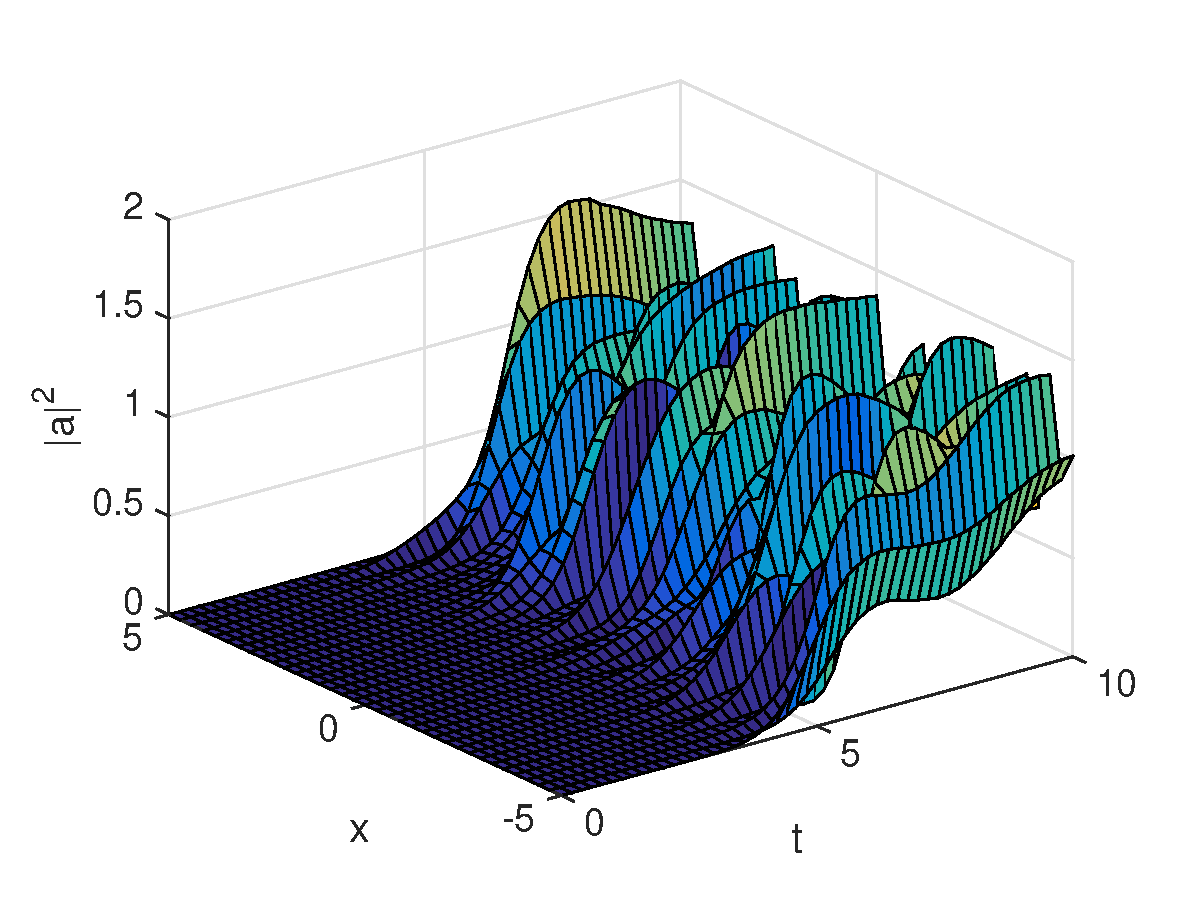
\includegraphics[width=0.75\textwidth]{GinzLand}

\caption{\label{fig:Symmetry-breaking}\emph{Simulation of the stochastic equation
describing symmetry breaking in two dimensions. Spatial fluctuations
are caused by the different phase-domains that interfere. The graph
obtained here is projected onto the $y=0$ plane.}}
\vspace{10pt}
 
\end{figure}


\subsection{NLS soliton}

The famous nonlinear Schrödinger equation (NLSE) is: 
\begin{equation}
\frac{da}{dt}=\frac{i}{2}\left[\nabla^{2}a-a\right]+ia\left|a\right|^{2}.
\end{equation}

Together with the initial condition that $a(0,x)=sech(x)$, this has
a soliton \cite{Scott1973soliton}, an exact solution that doesn't
change in time: 
\begin{eqnarray}
a(t,x) & = & sech(x).
\end{eqnarray}
The Fourier transform at $k=0$ is simply: 
\begin{eqnarray}
\tilde{a}(t,0) & = & \frac{1}{\sqrt{2\pi}}\int sech(x)dx=\sqrt{\frac{\pi}{2}}.
\end{eqnarray}


\subsection*{Exercises}
\begin{itemize}
\item \textbf{Solve the NLSE for a soliton using a function instead of a
script, then include an additive complex noise of $0.01(w_{1}+iw_{2}$)
to the differential equation, and plot again with an average over
$1000$ samples.} 
\end{itemize}
\newpage{}

\subsection{Planar noise}

The next example is growth of thermal noise of a two-component complex
field in a plane, given by the equation 
\begin{equation}
\frac{d\mathbf{a}}{dt}=\frac{i}{2}\nabla^{2}\mathbf{a}+\mathbf{w}(t,x).
\end{equation}
where $\mathbf{\zeta}$ is a delta-correlated complex noise vector
field: 
\begin{equation}
w_{j}(t,\mathbf{x})=\left[w_{j}^{re}(t,\mathbf{x})+i\zeta_{j}^{im}(t,\mathbf{x})\right]/\sqrt{2},
\end{equation}
with the initial condition that the initial noise is delta-correlated
in position space 
\begin{equation}
a(0,\mathbf{x})=\mathbf{\zeta}^{(in)}(\mathbf{x})
\end{equation}
where: 
\begin{equation}
\mathbf{\zeta}^{(in)}(\mathbf{x})=\left[\mathbf{\zeta}^{re(in)}(\mathbf{x})+i\mathbf{\zeta}^{im(in)}(\mathbf{x})\right]/\sqrt{2}
\end{equation}

This has an exact solution for the noise intensity in either ordinary
space or momentum space: 
\begin{eqnarray}
\left\langle \left|a_{j}\left(t,\mathbf{x}\right)\right|^{2}\right\rangle  & = & (1+t)/dV\nonumber \\
\left\langle \left|\tilde{a}_{j}\left(t,\mathbf{k}\right)\right|^{2}\right\rangle  & = & (1+t)/dV_{k}\nonumber \\
\left\langle \tilde{a}_{1}\left(t,\mathbf{k}\right)\tilde{a}_{2}^{*}\left(t,\mathbf{k}\right)\right\rangle  & = & 0.
\end{eqnarray}

Here, the noise is delta-correlated, and $dV$, $dV_{k}$ are the
cartesian space and momentum space lattice cell volumes, respectively.
Suppose that $n=n_{x}n_{y}$ is the total number of spatial points,
and there are $n_{x(y)}$ points in the x(y)-direction, so then: 
\begin{eqnarray}
dV & = & dxdy\\
dV_{k} & = & dk_{x}dk_{y}=\frac{(2\pi)^{2}}{ndV}.\nonumber 
\end{eqnarray}

In the simulations, two planar noise fields are propagated, one using
delta-correlated noise, the other with noise transformed to momentum
space to allow filtering. This allows use of finite correlation lengths
when needed, by including a frequency filter function that is used
to multiply the noise in Fourier-space. The Fourier-space noise variance
is the square of the filter function.

The first noise index, $p.noises(1)$, indicates how many noise fields
are generated, while $p.noises(2)$ indicates how many of these are
spatially correlated, via Fourier transform, filter and inverse Fourier
transform. These appear to the user as additional noises, so the total
is $p.noises(1)+p.noises(2)$. The filtered noises have a finite correlation
length. They are correlated with the first $p.noises(1)$ x-space
noises they are generated from, as this can be useful.

\subsection*{Exercises}
\begin{itemize}
\item \textbf{Solve the planar noise growth equation} 
\end{itemize}
\begin{center}
\doublebox{\begin{minipage}[t]{0.75\columnwidth}%
\texttt{function {[}e{]} = Planar()}

\texttt{p.name = 'Planar noise growth';}

\texttt{p.dimensions = 3;}

\texttt{p.fields = 2;}

\texttt{p.ranges = {[}1,5,5{]};}

\texttt{p.steps = 2;}

\texttt{p.noises = {[}2,2{]};}

\texttt{p.ensembles = {[}10,4,4{]};}

\texttt{p.initial = @Initial;}

\texttt{p.deriv = @Da;}

\texttt{p.linear = @Linear;}

\texttt{p.observe = @(a,p) a(1,:).{*}conj(a(1,:));}

\texttt{p.olabels = '\textless\textbar a\_1(x)\textbar\textasciicircum 2\textgreater
';}

\texttt{p.compare = @(p) {[}1+p.t{]}/p.dv;}

\texttt{p.images = 4;}

\texttt{e = xspde(p);}

\texttt{end }~\\
 \ 

\texttt{function a0 = Initial(v,p)}

\texttt{a0(1,:) = (v(1,:)+1i{*}v(2,:))/sqrt(2);}

\texttt{a0(2,:) = (v(3,:)+1i{*}v(4,:))/sqrt(2);}

\texttt{end }~\\
 \ 

\texttt{function da = Da(a,w,p)}

\texttt{da(1,:) = (w(1,:)+1i{*}w(2,:))/sqrt(2);}

\texttt{da(2,:) = (w(3,:)+1i{*}w(4,:))/sqrt(2);}

\texttt{end }~\\
 \ 

\texttt{function L = Linear(p)}

\texttt{lap = p.Dx.\textasciicircum 2+p.Dy.\textasciicircum 2;}

\texttt{L(1,:) = 1i{*}0.5{*}lap(:);}

\texttt{L(2,:) = 1i{*}0.5{*}lap(:);}

\texttt{end}%
\end{minipage}} 
\par\end{center}
\begin{itemize}
\item \textbf{Add a decay rate of $-a$ to the differential equation, then
plot again} 
\item \textbf{Add growth and nonlinear saturation terms} 
\end{itemize}

\subsection{Gross-Pitaevskii equation}

The next example is a stochastic Gross-Pitaevskii (GP) equation \cite{Gardiner2003Stochastic}
in two dimensions, 
\begin{equation}
\frac{da}{dt}=\frac{i}{2}\nabla^{2}a-ia(V(r)-i\kappa(r)+\left|a\right|^{2})+\epsilon\eta\label{eq:Stochastic GPE}
\end{equation}
where $\eta$ is a correlated complex noise vector field: 
\begin{equation}
\eta(t,\mathbf{x})=w_{1}(t,\mathbf{x})+iw_{2}(t,\mathbf{x}),
\end{equation}
with the initial condition that the initial random field and the noise
are both filtered in momentum space 
\begin{equation}
a(0,\mathbf{x})=a_{0}(\mathbf{x})+\epsilon\zeta^{(in)}(\mathbf{x})
\end{equation}
where: 
\begin{equation}
\zeta^{(in)}(\mathbf{x})=v_{1}(\mathbf{x})+iv_{2}(\mathbf{x})
\end{equation}

We add a Gaussian filter in momentum space for both the initial random
field and noise so that, if $\tilde{w}\left(\mathbf{k}\right)$ is
a delta-correlated noise in momentum space: 
\begin{align}
w\left(\mathbf{k}\right) & =\tilde{w}\left(\mathbf{k}\right)\exp\left(-\left|\mathbf{k}\right|^{2}\right)\nonumber \\
v\left(\mathbf{k}\right) & =\tilde{v}\left(\mathbf{k}\right)\exp\left(-\left|\mathbf{k}\right|^{2}\right)
\end{align}

This allows use of finite correlation lengths when needed, by including
a frequency filter function that is used to multiply the noise in
Fourier-space. The Fourier-space noise variance is the square of the
filter function.

The first noise index, $p.noises(1)$, indicates how many noise fields
are generated that are delta-correlated in $x$, while $p.noises(2)$
indicates how many of these are spatially correlated, via Fourier
transform, filter and inverse Fourier transform. These appear to the
user as additional noises, so the total is $p.noises(1)+p.noises(2)$.
The filtered noises have a finite correlation length.

\subsection*{Exercises}
\begin{itemize}
\item \textbf{Solve the stochastic GP equation \eqref{eq:Stochastic GPE},
with a noise coefficient of $b=0.1$, $V=0.01\left|\mathbf{x}\right|^{2},$
$\kappa=0.001\left|\mathbf{x}\right|^{4}$, and a stored output data
file.} 
\end{itemize}
\begin{center}
\doublebox{\begin{minipage}[t]{0.75\columnwidth}%
\texttt{function {[}e{]} = GPE()}

\texttt{p.name = 'GPE';}

\texttt{p.dimensions = 3;}

\texttt{p.points = {[}101,64,64{]};}

\texttt{p.ranges = {[}1,20,20{]};}

\texttt{p.noises = {[}0,2{]};}

\texttt{p.rfilter = @(w,p) w.{*}exp(-p.kx.\textasciicircum 2-p.ky.\textasciicircum 2);}

\texttt{p.nfilter = @(v,p) v.{*}exp(-p.kx.\textasciicircum 2-p.ky.\textasciicircum 2);}

\texttt{b = @(xi) .1{*}(xi(1,:,:)+1i{*}xi(2,:,:));}

\texttt{p.initial = @(v,p) (p.x+1i{*}p.y)./(1+10{*}(p.x.\textasciicircum 2
+...}

\texttt{p.y.\textasciicircum 2))+b(v);}

\texttt{V = @(p) 0.01{*}(p.x.\textasciicircum 2 + p.y.\textasciicircum 2)-0.001{*}1i{*}(p.x.\textasciicircum 2
+...}

\texttt{p.y.\textasciicircum 2).\textasciicircum 2;}

\texttt{p.deriv = @(a,w,p) -1i{*}a.{*}(V(p)+conj(a).{*}a)+b(w);}

\texttt{p.linear = @(p) 0.5{*}1i{*}(p.Dx.\textasciicircum 2+p.Dy.\textasciicircum 2);}

\texttt{p.observe\{1\} = @(a,p) a.{*}conj(a);}

\texttt{p.images = \{2\};}

\texttt{p.imagetype = \{2\};}

\texttt{p.olabels = \{'\textbar a\textbar\textasciicircum 2'\};}

\texttt{p.file = 'GPE.mat';}

\texttt{e = xsim(p);}

\texttt{xgraph(p.file,p);}

\texttt{end}%
\end{minipage}} 
\par\end{center}

\newpage{}

\subsection{Characteristic equation}

The next example is the characteristic equation for a traveling wave
at constant velocity \cite{courant2008methods}. It is included to
illustrate what happens at periodic boundaries, when Fourier-transform
methods are used for propagation. There are a number of methods known
to prevent this effect, including addition of absorbers - called apodization
- at the boundaries. The equation is: 
\begin{equation}
\frac{da}{dt}+\frac{da}{dx}=0.
\end{equation}

Together with the initial condition that $a(0,x)=sech(2x+5)$, this
has an exact solution that propagates at a constant velocity: 
\begin{eqnarray}
a(t,x) & = & sech(2(x-t)+5).
\end{eqnarray}
The time evolution at $x=0$ is simply: 
\begin{eqnarray}
a(t,0) & = & sech(2(t-5/2)).
\end{eqnarray}


\subsection*{Exercises}
\begin{itemize}
\item \textbf{Solve the characteristic equation given above, noting the
effects of periodic boundaries.} 
\end{itemize}
\begin{center}
\doublebox{\begin{minipage}[t]{0.75\columnwidth}%
\texttt{function {[}e{]} = Characteristic()}

\texttt{p.name = 'Characteristic';}

\texttt{p.dimensions = 2;}

\texttt{p.initial = @(v,p) sech(2.{*}(p.x+2.5));}

\texttt{p.deriv = @(a,z,p) 0{*}a;}

\texttt{p.linear = @(p) -p.Dx;}

\texttt{p.olabels = \{'a\_1(x)'\};}

\texttt{p.compare = @(p) sech(2.{*}(p.t-2.5));}

\texttt{e = xspde(p);}

\texttt{end}%
\end{minipage}} 
\par\end{center}
\begin{itemize}
\item \textbf{Recalculate with the opposite velocity, and a new exact solution.} 
\end{itemize}

\subsection{Nonlinear Anderson localization}

A random potential \emph{prevents} normal wave-packet spreading in
quantum-mechanics. This is Anderson localization \cite{Anderson1958Absence}:
a famous property of quantum mechanics in a random potential. A typical
experimental method is to confine an ultra-cold Bose-Einstein condensate
(BEC) in a trap, then release the BEC in a random external potential
produced by a laser \cite{billy2008direct}. The expansion rate of
the BEC is reduced by the Anderson localization due to the random
potential. Physically, the observable quantity is the particle density
$n=\left|\psi\right|^{2}$, but there is a complication, which is
that there are nonlinearities from atomic scattering \cite{pikovsky2008destruction}.

This can be treated either using a Schrodinger equation with a random
potential, at low density, or using the Gross-Pitaevskii (GP) equation
to include atom-atom interactions at the mean field level. In this
example of a problem where strong localization occurs, the general
equations are:

\begin{equation}
\frac{\partial\psi}{\partial t}=\frac{1}{i\hbar}\left[-\frac{\hbar^{2}}{2m}\nabla^{2}+V\left(\mathbf{r}\right)+g\left|\psi\right|^{2}\right]\psi.
\end{equation}

In calculations, it is best to use a dimensionless form by rescaling
coordinates and fields. A simple way to simulate this with xSPDE is
to treat $\psi$ as a scaled field $a(1),$ and to assume the random
potential field $V\left(\mathbf{r}\right)$ as caused by interactions
with second random field $\left|a(2)\right|^{2}$. This has the advantage
that it is similar to the actual experiment and allows one to treat
time-dependent potentials as well, if desired.

With the rescaling, this simplifies to: 
\begin{equation}
\frac{\partial a_{1}}{\partial\tau}=i\left[\frac{\partial}{\partial\zeta^{2}}^{2}-\left|a_{2}\right|^{2}-\left|a_{1}\right|^{2}\right]a_{1}.
\end{equation}

A convenient initial condition is to use: 
\begin{eqnarray}
a_{1} & = & a_{0}\exp(-\zeta^{2})\nonumber \\
\left\langle a_{2}(\zeta)a_{2}(\zeta')\right\rangle  & = & v\delta\left(\zeta-\zeta'\right).
\end{eqnarray}


\subsection*{Exercise}
\begin{itemize}
\item \textbf{Solve Schrodinger's equation without a random potential, to
observe expansion.} 
\item \textbf{Include a random potential $v$, to observe localization.} 
\item \textbf{Experiment with nonlinear terms and higher dimensions.} 
\end{itemize}
The GP equation is a mean field approximation; this is still not a
full solution of the many-body problem! Also, the experiments are
more complicated than this, and actually observe the momentum distribution.

\newpage{}

\part{Methods, API and Examples}

\chapter{Stochastic methods and errors\label{sec:Algorithms}}

\textbf{\emph{This chapter describes the methods available, and how
to add custom algorithms.}}

\section{Introduction to algorithms}

Stochastic, partial and ordinary differential equations are central
to numerical mathematics. Ordinary differential equations have been
known in some form ever since calculus was invented. There are an
extraordinary number of algorithms used to solve these equations.
This chapter provides an overview of the included algorithms.\\
 xSPDE has six built-in choices of algorithm, with defaults. All built-in
methods have an interaction picture and can be used with any space
dimension, including $dimensions=1$, which is an ordinary stochastic
equation. All can be used with stochastic or with non-stochastic equations,
and with order extrapolation. \\
 For stochastic equations, the Euler method requires an Ito form of
stochastic equation, the implicit Euler method requires an implicit
Ito form, while the others should be used with the Stratonovich form
of calculus. Each is chosen to be able to use an interaction picture
to take care of exactly soluble linear terms.

The default methods will solve most DE, SDE, PDE and SPDE problems
reliably, but other ones can be included if needed.

\subsection{Standard methods}

The standard xSIM algorithms given below are available for ODEs, PDEs,
SDEs and SPDEs. More advanced algorithms for specialized cases are
described in section \ref{sec:Algorithms}.

For stochastic differential equations, which are non-differentiable,
the usual rules of calculus do not apply because stochastic noise
is non-differentiable. It has fluctuations proportional to $1/\sqrt{dtdV}$,
for noise defined on a lattice with temporal cell-size $dt$ and spatial
cell-size $dV$. Hence, the usual differentiability and smoothness
properties required to give high-order convergence for standard Runge-Kutta
methods are simply not present. Instead, xSPDE has a built-in extrapolation
to zero step-size for high-order stochastic convergence.

Many more complex higher order algorithms for stochastic integration
exist but are not included in the current xSPDE distribution, and
users are encouraged to contribute their favorite methods.

We note here that there are multiple error sources possible. SDE/SPDE
errors are often dominated by the sampling error, not discretization.
In addition, all convergence theorems only apply to the limit of zero
step-size. One may be very far from this regime in a given practical
calculation. Analytic error estimates also have prefactors which are
hard to calculate. However, xSPDE can numerically estimate both the
discretization and sampling error for any given average observable.

\subsection{Advanced methods}

Three more advanced method libraries are included here, namely \emph{weighted},
\emph{projected} and \emph{forward-backward} stochastic differential
equations. If you have a favorite algorithm that is not included,
user-defined algorithms and libraries can be added. The existing methods
are listed below, and the corresponding {.m}-files can be used as
a model.

Define the routine, for example {"myalgorithm.m"}, set \textit{$p.method=@myalgorithm$},
then adjust the input value of \emph{ipsteps} and \emph{order} if
these need be changed to a new value. The interaction-picture transform,
\emph{prop}, can also be changed if the built-in choice is not sufficient.The
xSPDE algorithms available currently treat 
\begin{itemize}
\item ordinary (and partial) differential equations 
\item stochastic differential equations 
\item stochastic partial differential equations 
\item weighted stochastic differential equations 
\item projected stochastic differential equations, 
\item forward-backward stochastic differential equations 
\end{itemize}
Some of the more advanced features of the libraries require additional
input parameters. In particular: 
\begin{description}
\item [{backfields}] is used for forward-backward stochastic equations,
describing backward time components. These are described in the \emph{Forward-backward}
section. Note that \textbf{fields} is still used, and it gives the
total number of forward+backward fields. 
\item [{auxfields}] gives the number of auxiliary fields. These have a
functional definition (\emph{defines}) that includes both a field
and noise variable, as needed for spectral observables. Cell index
numbers $i$ greater than the maximum field cells access the auxiliary
fields in the \emph{observe} function. 
\end{description}

\section{General differential form}

The general equation treated is given in differential form as 
\begin{equation}
\begin{split}\frac{\partial\boldsymbol{a}}{\partial t}=\boldsymbol{A}\left[\boldsymbol{\nabla},\boldsymbol{a},t\right]+\underline{\mathbf{B}}\left[\boldsymbol{\nabla},\boldsymbol{a},t\right]\cdot\boldsymbol{\zeta}(t)+\underline{\mathbf{L}}\left[\boldsymbol{\nabla}\right]\cdot\boldsymbol{a}.\end{split}
\label{eq:Standard xspde SDE}
\end{equation}
It is convenient for the purposes of describing interaction picture
methods, to introduce an abbreviated notation as: 
\begin{equation}
\begin{split}\begin{aligned}\mathcal{D}\left[\mathbf{a},t\right]=\boldsymbol{A}\left[\boldsymbol{a},t\right]+\underline{\mathbf{B}}\left[\boldsymbol{a},t\right]\cdot\boldsymbol{\zeta}(t).\end{aligned}
\end{split}
\end{equation}
Hence, we can rewrite the differential equation in the form: 
\begin{equation}
\begin{split}\frac{\partial\boldsymbol{a}}{\partial t}=\mathcal{D}\left[\mathbf{a},t\right]+\underline{\mathbf{L}}\left[\boldsymbol{\nabla}\right]\cdot\boldsymbol{a}.\end{split}
\end{equation}


\subsection{Linear propagator}

Next, we define a linear propagator. This is given formally by: 
\begin{equation}
\begin{split}\mathcal{P}\left(\Delta t\right)=\exp\left(\Delta t\underline{\mathbf{L}}\left[\boldsymbol{\nabla}\right]\right)\end{split}
.
\end{equation}
Typically, but not necessarily, this is evaluated in Fourier space,
where it should be just a diagonal term in the momentum vector conjugate
to the transverse space coordinate. It will then involve a Fourier
transform, multiplication by an appropriate function of the momentum,
and then an inverse Fourier transform afterwards. For simplicity,
the stochastic noise is assumed constant throughout the interval $dt$.
The reader is referred to the literature for more details.

It is simple to add your own algorithm if you prefer a different one.
Note that if they use an interaction picture, then \emph{ipsteps}
must be given explicitly to specify the interaction picture duration,
where \emph{ipsteps} gives the number of sequential propagator steps
in time required for the method.

\section{Standard methods}

The standard methods are listed below. All of these can be used with
any equation: ODE, SDE, PDE or SPDE, either with or without a linear
interaction picture term.

\subsection{\emph{Euler}: Ito-Euler}

\label{algorithms:euler} This is an explicit Ito-Euler method using
an interaction picture. While traditional, it is not generally recommended.
If it is used, very small step-sizes will generally be necessary to
reduce errors to a usable level. This is because it is is only convergent
to first order deterministically and tends to have large errors.

It is designed for use with an Ito form of stochastic equation. It
requires one IP transform per step (\textit{$p.ipsteps=1$}). Starting
from time $t=t_{n}$, to get the next time point at $t=t_{n+1}=t_{n}+\Delta t$,
one calculates: 
\begin{equation}
\begin{split}\begin{aligned}\Delta\mathbf{a}_{n} & =\Delta t\mathcal{D}\left[\mathbf{a}_{n},t_{n}\right]\\
\mathbf{a}_{n+1} & =\mathcal{P}\left(\Delta t\right)\cdot\left[\mathbf{a}_{n}+\Delta\mathbf{a}_{n}\right]
\end{aligned}
\end{split}
\end{equation}


\subsection{\emph{Implicit}: implicit Ito-Euler}

\label{algorithms:implicit} This is a fully implicit Ito-Euler method
using an interaction picture. It is more robust, though slower, than
the explicit form. If it is used, very small step-sizes will generally
be necessary to reduce errors to a usable level.

This is because it is is only convergent to first order, and therefore
tends to have large errors. It is designed for use with an implicit
Ito form of stochastic equation. Note that this implies double the
usual Stratonovich correction!

It requires one IP transform per step ($p.ipsteps=1$). Starting from
time $t=t_{n}$, to get the next time point at $t=t_{n+1}=t_{n}+\Delta t$,
one calculates, using iteration to get the implicit result of the
next time-point:

\begin{equation}
\begin{split}\begin{aligned}\bar{\mathbf{a}}^{(0)} & =\mathcal{P}\left(\Delta t\right)\cdot\left[\mathbf{a}_{n}\right]\\
\bar{\mathbf{a}}^{(i)} & =\bar{\mathbf{a}}^{(0)}+\Delta t\mathcal{D}\left[\bar{\mathbf{a}}^{(i-1)},t_{n+1}\right]\\
\mathbf{a}_{n+1} & =\bar{\mathbf{a}}^{(iter)}
\end{aligned}
\end{split}
\end{equation}
\begin{equation}
\begin{split}\begin{aligned}\tilde{\mathbf{a}}_{n} & =\mathcal{P}\left(\Delta t\right)\cdot\left[\mathbf{a}_{n}\right]\\
\Delta\mathbf{a}_{n} & =\Delta t\mathcal{D}\left[\tilde{\mathbf{a}}_{n}+\Delta\mathbf{a}_{n},t_{n}\right]\\
\mathbf{a}_{n+1} & =\tilde{\mathbf{a}}_{n}+\Delta\mathbf{a}_{n}
\end{aligned}
\end{split}
\end{equation}


\subsection{\emph{MP}: Midpoint}

\label{algorithms:midpoint} This is a semi-implicit midpoint method
using an interaction picture. It gives good results for stochastic
and stochastic partial differential equations. It is convergent to
second order in time for deterministic equations and for stochastic
equations with commuting noise. It is strongly convergent and robust.
It requires two half-length IP transforms per step ($p.ipsteps=2$).

To get the next time point, one calculates a midpoint derivative iteratively
at time to get the next time point at $t=t_{n+1/2}=t_{n}+\Delta t/2$,
to give an estimated midpoint field $\bar{\mathbf{a}}^{(i)}$, usually
with four iterations. The number of iterations can be changed: 
\begin{equation}
\begin{split}\begin{aligned}\bar{\mathbf{a}}^{(0)} & =\mathcal{P}\left(\frac{\Delta t}{2}\right)\cdot\left[\mathbf{a}_{n}\right]\\
\bar{\mathbf{a}}^{(i)} & =\bar{\mathbf{a}}^{(0)}+\frac{\Delta t}{2}\mathcal{D}\left[\bar{\mathbf{a}}^{(i-1)},t_{n+1/2}\right]\\
\mathbf{a}_{n+1} & =\mathcal{P}\left(\frac{\Delta t}{2}\right)\cdot\left[2\bar{\mathbf{a}}^{(iter)}-\bar{\mathbf{a}}^{(0)}\right]
\end{aligned}
\end{split}
\end{equation}

This is the default method for stochastic cases.

\subsection{\emph{MPadap}t: adaptive midpoint}

\label{algorithms:midpoint-1} This is an implicit midpoint method
using an interaction picture, together with an adaptive technique
for integrating highly nonlinear equations. At low amplitudes it is
identical to the standard midpoint method. For amplitudes $|a_{i}|^{2}$
above a critical value, \emph{p.adapt}, the amplitude is inverted
and propagated using the differential equation for its inverse.

Initially a switch $p$ is set to $1$ for low amplitudes, and $-1$
for high amplitudes. To get the next time point, one calculates a
midpoint derivative iteratively at time to get the next time point
at $t=t_{n+1/2}=t_{n}+\Delta t/2$, to give an estimated midpoint
field $\bar{\mathbf{a}}^{(i)}$, as above, but with the derivative
modified to give the derivative of $a_{i}^{p}$: 
\begin{equation}
\begin{split}\begin{aligned}\bar{\mathbf{a}}^{(0)} & =\mathcal{P}\left(\frac{\Delta t}{2}\right)\cdot\left[\mathbf{a}_{n}\right]\\
\tilde{\mathbf{a}}^{(0)} & =\mathbf{a}_{n}^{p}\\
\tilde{\mathbf{a}}^{(i)} & =\tilde{\mathbf{a}}^{(0)}+\frac{\Delta t}{2}p\left[\tilde{\mathbf{a}}^{(i-1)}\right]{}^{1-p}\left(\mathcal{D}\left[[\tilde{\mathbf{a}}^{(i-1)}]^{p},t_{n+1/2}\right]\right)\\
\mathbf{a}_{n+1} & =\mathcal{P}\left(\frac{\Delta t}{2}\right)\cdot\left[2\tilde{\mathbf{a}}^{(iter)}-\tilde{\mathbf{a}}^{(0)}\right]^{p}
\end{aligned}
\end{split}
\end{equation}


\subsection{\emph{RK2}: second order Runge-Kutta}

\label{algorithms:second-order-runge-kutta} This is a second order
Runge-Kutta method using an interaction picture. It is convergent
to second order in time for non-stochastic equations, and for stochastic
equations with additive noise, but otherwise it is first order. It
often has higher errors than midpoint methods. It requires two IP
transforms per step, but each is a full time-step long ($p.ipsteps=1$).

To get the next time point, one calculates: 
\begin{equation}
\begin{split}\begin{aligned}\bar{\mathbf{a}} & =\mathcal{P}\left(\Delta t\right)\cdot\left[\mathbf{a}_{n}\right]\\
\mathbf{d}^{(1)} & =\Delta t\mathcal{P}\left(\Delta t\right)\cdot\mathcal{D}\left[\mathbf{a}_{n},t_{n}\right]\\
\mathbf{d}^{(2)} & =\Delta t\mathcal{D}\left[\bar{\mathbf{a}}+\mathbf{d}^{(1)},t_{n+1}\right]\\
\mathbf{a}_{n+1} & =\bar{\mathbf{a}}+\left(\mathbf{d}^{(1)}+\mathbf{d}^{(2)}\right)/2.
\end{aligned}
\end{split}
\end{equation}


\subsection{\emph{RK4}: fourth order Runge-Kutta}

\label{algorithms:fourth-order-runge-kutta} This is a fourth order
Runge-Kutta method using an interaction picture. It is convergent
to fourth order in time for non-stochastic equations, but for stochastic
equations it can be more slowly convergent than the midpoint method.
It requires four half-length IP transforms per step (\emph{ipsteps}
= 2). To get the next time point, one calculates four derivatives
sequentially: 
\begin{equation}
\begin{split}\begin{aligned}\bar{\mathbf{a}} & =\mathcal{P}\left(\frac{\Delta t}{2}\right)\cdot\left[\mathbf{a}_{n}\right]\\
\mathbf{d}^{(1)} & =\frac{\Delta t}{2}\mathcal{P}\left(\frac{\Delta t}{2}\right)\cdot\mathcal{D}\left[\mathbf{a}_{n},t_{n}\right]\\
\mathbf{d}^{(2)} & =\frac{\Delta t}{2}\mathcal{D}\left[\bar{\mathbf{a}}+\mathbf{d}^{(1)},t_{n+1/2}\right]\\
\mathbf{d}^{(3)} & =\frac{\Delta t}{2}\mathcal{D}\left[\bar{\mathbf{a}}+\mathbf{d}^{(2)},t_{n+1/2}\right]\\
\mathbf{d}^{(4)} & =\frac{\Delta t}{2}\mathcal{D}\left[\mathcal{P}\left(\frac{\Delta t}{2}\right)\left[\bar{\mathbf{a}}+2\mathbf{d}^{(3)},t_{n+1}\right]\right]\\
\mathbf{a}_{n+1} & =\mathcal{P}\left(\frac{\Delta t}{2}\right)\cdot\left[\bar{\mathbf{a}}+\left(\mathbf{d}^{(1)}+2\left(\mathbf{d}^{(2)}+\mathbf{d}^{(3)}\right)\right)/3\right]+\mathbf{d}^{(4)}/3
\end{aligned}
\end{split}
\end{equation}
This might seem the obvious choice, having the highest order. However,
it can converge at a range of apparent rates, depending on the relative
importance of stochastic and non-stochastic terms. Due to its use
of differentiability, it may converge more slowly than the midpoint
method with stochastic terms present. It is the default for ODE and
PDE cases.

\section{Weighted library}

In some types of stochastic equation, there is a weight associated
with each trajectory, which is used to weight the probability of the
trajectory \cite{kiesewetter2022coherent}. This type of equation
is sometimes found when dealing with quantum trajectories \cite{Dalibard1992Wave,Carmichael1993Quantum}
and feedback \cite{Hush2013Controlling}.

The equations still have the standard form of Eq \eqref{eq:SDE},
with an extra weight equation, Eq \eqref{eq:SDE-2}. However, the
results for mean values are weighted by a term $\exp\left(\Omega\left(t\right)\right)$,
so that: 
\begin{equation}
\left\langle \mathbf{O}\right\rangle _{\Omega}=\frac{\sum_{n}\mathbf{O}\left(\mathbf{a}^{\left(n\right)}\right)\exp\left(\Omega^{\left(n\right)}\left(t\right)\right)}{\sum_{n}\exp\left(\Omega^{\left(n\right)}\left(t\right)\right)}.\label{eq:Weighted-averages}
\end{equation}

This reduces to the standard expression of Eq \eqref{eq:averages-1}
in the case that $\Omega\left(t\right)=0$. To simulate these equations
automatically, the weight exponent $\Omega$ is integrated as the
\emph{last} field in the vector $\mathbf{a}$, which must have at
least two components. A nonzero threshold weight, $thresholdw$, must
be entered to allow calculation of breeding.

With these changes, averages in each vector ensemble are calculated
using Eq \eqref{eq:Weighted-averages}. Before each plotted step in
the calculation, a breeding calculation is carried out. There are
$p.steps(1)-1$ of these in total. During breeding, any weight such
that $\exp\left(\Omega^{(n)}\right)<thresholdw/\left\langle \exp\left(\Omega\right)\right\rangle $
is removed.

The most probable trajectory is then duplicated to replace the low-weight
trajectory. Both exponential weights are halved, so the total weight
of the remaining trajectories is unchanged. If they are complex, weights
such that $\exp\left(Re\left(\Omega^{(n)}\right)\right)<thresholdw/\left\langle \exp\left(Re\left(\Omega\right)\right)\right\rangle $
are removed, and the real weight of the bred trajectory is reduced,
which removes any low-weight trajectories that don't contribute. When
used, the internal variable \emph{p.breedw }is set to allow the fraction
of trajectories that are bred per step to be monitored. For weighted
SPDEs, the spatial weights $\Omega(x_{j})$ are summed over space
points to obtain $\Omega$.

\subsection{Example}

The following example shows how weights are implemented. 
\begin{center}
\doublebox{\begin{minipage}[t]{0.75\columnwidth}%
\texttt{function {[}e{]} = Weightcheck()}

\texttt{p.name = 'Weightcheck';}

\texttt{p.ensembles = {[}10000,10,1{]};}

\texttt{p.fields = 2;}

\texttt{p.points = 6;}

\texttt{p.order = 2;}

\texttt{p.thresholdw = 0.1;}

\texttt{p.diffplot = 1;}

\texttt{p.initial = @(w,p) {[}1+w(1,:);0{*}w(2,:){]};}

\texttt{p.deriv = @(a,z,p) {[}-a(1,:)+ z(1,:);-a(2,:)+...}

\texttt{z(2,:){]};}

\texttt{p.observe\{1\} = @(a,p) a(1,:);}

\texttt{p.observe\{2\} = @(a,p) p.breedw;}

\texttt{p.compare\{1\} = @(p) exp(-p.t);}

\texttt{p.olabels\{1\} = '\textless a\textgreater ';}

\texttt{p.olabels\{2\} = '\textless fractional breeds per step\textgreater
';}

\texttt{e = xcheck(2,p);}

\texttt{end}%
\end{minipage}} 
\par\end{center}

This algorithm converges with second-order accuracy for this exercise,
due to the structure of the equation. The example also demonstrates
how to use the \emph{xcheck} function instead of \emph{xspde}, to
check convergence.

\section{Projection library}

It is sometimes necessary to constrain an equation to a sub-manifold
\cite{Joseph2023midpoint}, with an equation of form: 
\begin{equation}
\mathbf{f}\left(\mathbf{a}\right)=0,
\end{equation}
where $\mathbf{f}\left(\mathbf{a}\right)$ is a scalar or vector function
that defines the relevant manifold in Euclidean space. The projected
SDE then has the form of a Stratonovich SDE, where: 
\begin{equation}
\frac{\partial\mathbf{a}}{\partial t}=\mathcal{P}_{\mathbf{a}}^{\parallel}\left[\mathbf{A}\left[\mathbf{a}\right]+\underline{\mathbf{B}}\left[\mathbf{a}\right]\cdot\mathbf{w}(t)\right]\,,
\end{equation}
where $\mathcal{P}_{\mathbf{a}}^{\parallel}$ is a tangential projection
operator at location $\mathbf{a}$ on the sub-manifold, and as usual,
$\mathbf{A}$ is a vector, $\underline{\mathbf{B}}$ a matrix and
$\mathbf{w}$ is a real Gaussian noise vector, delta-correlated in
time. Similarly, the general stochastic partial differential equation
can be written in projected form as

\begin{equation}
\frac{\partial\mathbf{a}}{\partial t}=\mathcal{P}_{\mathbf{a}}^{\parallel}\left[\mathbf{A}\left[\mathbf{a}\right]+\underline{\mathbf{B}}\left[\mathbf{a}\right]\cdot\mathbf{w}(t,\mathbf{x})+\underline{\mathbf{L}}\left[\mathbf{\nabla},\mathbf{a}\right]\,\right].
\end{equation}

When numerically integrating these, it is also useful to have a normal
projection $\mathcal{P}^{\perp}$available. This is used to normally
project to the nearest point on the manifold, to eliminate constraint
errors. These are solved using functions collected in a projection
library, to provide the specialized methods that are needed for this
purpose.

The projection library has three predefined algorithms, 
\begin{itemize}
\item \textbf{\emph{Enproj}},\emph{ } 
\item \textbf{\emph{MPproj}}, 
\item \textbf{\emph{MPnproj}}. 
\end{itemize}
Here the capital E stands for Euler, MP for midpoint. All use tangential
projection. The letter \emph{n=normal} indicates if an additional
normal projection is used. In all cases, if it is present, a normal
projection is used last. The recommended type is \textbf{\emph{MPnproj}},
due to its much lower errors.

Tangential and normal projections are needed to define the geometry
of any sub-manifold. These are input by setting the variable \emph{project}
equal to a function handle that defines the projection. These can
be user provided if required. There are three different predefined
manifold geometry types, which need different inputs, given below.

\subsection{Calling the \emph{project} function}

The calling arguments for the \emph{project} function are: \emph{(d,a,n,p)},
where d is a vector to be tangentially projected at location a, a
is the current (near)-manifold location, n is an option switch, and
p is the parameter structure.

The options available in any \emph{project} implementation are defined
as: 
\begin{itemize}
\item \textit{n = 0} returns the tangent vector for testing 
\item \textit{n = 1} returns the tangential projection of \emph{d} at \emph{a} 
\item \textit{n = 2} returns the normal projection of \emph{a}, where \emph{d}
is not used 
\item \textit{n = 4} returns the constraint function at \emph{a} for testing 
\end{itemize}
The projections defined in an xSPDE \emph{project} function can be
of any type. Arbitrary dimension reduction and manifold geometry is
possible. Currently in the examples, dimensionality is reduced by
1, and normal projections use fixed point iterations, defined by \emph{iterproj}.

\subsection{The predefined manifold geometries}

The current manifolds, by setting p.project = @Quadproj ..., are as
follows: 
\begin{enumerate}
\item Quadratic - \emph{Quadproj} - needs: \emph{qcproj} defined by $f=\sum q{}_{ij}x^{i}x^{j}-1=0$ 
\item Polynomial - \emph{Polproj} - needs: \emph{vcproj} defined by $f=\sum v_{i}(x^{i})^{p}-1=0$ 
\item Catenoid - \emph{Catproj} - uses fixed coefficients defined by $f=(x_{1})^{2}+(x_{2})^{2}-(sinh(x_{3}))^{2}-1=0$ 
\end{enumerate}
Any other manifold can be used by replacing these predefined manifolds
with an appropriate \emph{project} function.

\section{Forward-backward library}

The xSPDE forward-backward library implements an iterative stochastic
method which propagates an SDE or PSDE forward and backward in time.
This is used to treat Q-function phase-space methods, which do not
have a positive-definite diffusion \cite{Drummond2020Retrocausal}.
The iteration converges in simple cases, typically with no cross-coupling
apart from boundary conditions. It uses the algorithm \emph{MPfb.}

The general FB equations have the following structure, written as
an integral equation to make it clear what the relevant boundary conditions
are:

\begin{align}
\mathbf{p}\left(t\right) & =\mathbf{p}\left(0,\mathbf{q}\left(0\right)\right)+\int_{0}^{t}\left\{ \mathbf{A}^{p}\left[\mathbf{a}\left(t'\right)\right]dt'+\underline{\mathbf{B}}^{p}\left[\mathbf{a}\left(t'\right)\right]\cdot d\mathbf{w}^{p}(t')\right\} \nonumber \\
\mathbf{q}\left(t\right) & =\mathbf{q}\left(T,\mathbf{p}\left(T\right)\right)+\int_{t}^{T}\left\{ \mathbf{A}^{q}\left[\mathbf{a}\left(t'\right)\right]dt'+\underline{\mathbf{B}}^{q}\left[\mathbf{a}\left(t'\right)\right]\cdot d\mathbf{w}^{q}(t')\right\} .
\end{align}
Here, $\mathbf{a}=\left[\mathbf{p},\mathbf{q}\right]$ includes forward
components $\mathbf{p}$ and backwards components $\mathbf{q}$. These
have ``initial'' conditions in the past and the future, respectively,
and can depend on random inputs, just as with ordinary stochastic
equations.

The library includes the \emph{xpathfb} function which replaces the
\emph{xpath} function, which is used automatically. However, the user
must specify a modified step integrator, either \emph{Eulerfb} or
\emph{MPfb}. The \emph{initial} and deriv routines require additional
arguments, which are described in the table below, and are used during
the iteration scheme.

The noise terms $\mathbf{w}=\left[\mathbf{w}^{p},\mathbf{w}^{q}\right]$
are uncorrelated real Gaussian noises: 
\begin{equation}
\left\langle dw_{i}^{\alpha}\left(\mathbf{x}\right)dw_{j}^{\beta}\left(\mathbf{x}'\right)\right\rangle =\delta_{ij}\delta_{\alpha\beta}dt.
\end{equation}
This is solved in differential form, where $t_{-}=T-t$, as: 
\begin{align}
\frac{\partial\mathbf{p}}{\partial t} & =\mathbf{A}^{p}\left[\mathbf{a}\right]+\underline{\mathbf{B}}^{p}\left[\mathbf{a}\right]\cdot\mathbf{w}^{p}(t)\,\nonumber \\
\frac{\partial\mathbf{q}}{\partial t_{-}} & =\mathbf{A}^{q}\left[\mathbf{a}\right]+\underline{\mathbf{B}}^{q}\left[\mathbf{a}\right]\cdot\mathbf{w}^{q}(t)\,.
\end{align}

Each equation is solved by iteration. The previous value of the counter-propagating
field, ie $\mathbf{a}^{(n-1)}$, is used to solve for $\mathbf{a}^{(n)}$
in step $n$, since the current value is not yet known. That is, the
algorithm is: 
\begin{align}
\frac{\partial\mathbf{p}^{(n)}}{\partial t} & =\mathbf{A}^{p}\left[\mathbf{p}^{(n)}\left(t\right),\mathbf{q}^{(n-1)}\left(t\right)\right]+\underline{\mathbf{B}}^{p}\left[\mathbf{p}^{(n)}\left(t\right),\mathbf{q}^{(n-1)}\left(t\right)\right]\cdot\mathbf{w}^{p}\left(t\right)\,\\
\frac{\partial\mathbf{q}^{(n)}}{\partial t_{-}} & =\mathbf{A}^{q}\left[\mathbf{p}^{(n-1)}\left(t_{-}\right),\mathbf{q}^{(n)}\left(t_{-}\right)\right]+\underline{\mathbf{B}}^{q}\left[\mathbf{p}^{(n-1)}\left(t_{-}\right),\mathbf{q}^{(n)}\left(t_{-}\right)\right]\cdot\mathbf{w}^{q}\left(t_{-}\right)\,,\nonumber 
\end{align}
Convergence is the responsibility of the user, and the algorithm has
a fixed number of iterations. The starting point of the iteration
is the path function $fbfirst$. The simulation requires the following
additional inputs, including $backfields$, defining the backward
components. 
\begin{center}
\begin{tabular}{|c|c|c|c|}
\hline 
Label  & Type  & Typical value  & Description\tabularnewline
\hline 
\hline 
\emph{backfields}  & integer vector  & $1$  & Number of backward variables\tabularnewline
\hline 
\emph{initialfb}  & function handle  & $@(a0,a1,w,p)$  & Initial value for $a$\tabularnewline
\hline 
\emph{firstfb}  & function handle  & $@(a0,nc,p)$  & First trajectory estimate\tabularnewline
\hline 
\emph{iterfb}  & integer  & 2  & Forward-backward iterations\tabularnewline
\hline 
\emph{method}  & function handle  & $@xMPfb$  & Forward-backward algorithm\tabularnewline
\hline 
\emph{deriv}  & function handle  & \texttt{$@(a,a_{-},w,p)$}  & Derivative function\tabularnewline
\hline 
\end{tabular}\\
\par\end{center}

In \emph{initialfb}, the $a0$ fields from the previous iteration
are at the \emph{first} times computed previously, so $\mathbf{a}0=\left[\mathbf{p}^{(n-1)}\left(0\right),\mathbf{q}^{(n-1)}\left(T\right)\right]$,
while the $a1$ fields are evaluated at the \emph{last} times computed
from the previous iteration, so $\mathbf{a}1=\left[\mathbf{p}^{(n-1)}\left(T\right),\mathbf{q}^{(n-1)}\left(0\right)\right]$.

On the first call to \emph{initialfb, with }$p.iter=1$, a startup
procedure is used. In the startup procedure, \emph{a0} is generated
internally by \emph{initialfb. }However, \emph{a1} is obtained in
the internal calling function \emph{xpathfb} using the output of \emph{firstfb,}
which gives an initial iterative path estimate of $a$. It returns
a default path equal to the initial boundary value $a0$, if not defined
by the user. More generally, it should be set to a value to allow
iterations to converge. The calling arguments of \emph{firstfb} include
the initial boundaries \emph{a0} and the usual check index ($nc=1,2$).

The \emph{initial} function returns $a0$, giving the current initial
values. On the first iteration \emph{initial} returns an internally
defined $a0$. Subsequently it requires $a0$, the stored first iteration
boundaries as well as \emph{a1}, the previous iteration end-points.
The estimate for the previous path in the deriv function is obtained
from the iteration starter function\emph{ firstfb} on the first iteration,
and subsequently from a stored value.

Internally, the raw fields $\mathbf{a}=\left[\mathbf{p},\mathbf{q}\right]$
are stored in complementary time-orders, with $\mathbf{p}$ solved
normally in forward time, and $\mathbf{q}$ solved in reverse temporal
order.

When the previous iteration field is passed to $deriv$, the time-orders
of the previous iteration are reversed so that previous iteration
$\mathbf{q}$ times are the same as $\mathbf{p}$ times, and vice-versa.
The previous fields are therefore at the same time as those of the
complementary present field\emph{.} When passed to $observe$, both
$\mathbf{p},\mathbf{q}$ are given in time-increasing order to allow
synchronized observations.

\subsection{Example:}

This is a trivial example, to illustrate the code structure. It has
two counter-propagating stochastic processes, one decaying in the
forward time direction, and one decaying in the backward time direction. 
\begin{center}
\doublebox{\begin{minipage}[t]{0.75\columnwidth}%
\texttt{function {[}e{]} = Fbcheck()}

\texttt{p.ranges = 1;}

\texttt{p.fields = 2;}

\texttt{p.backfields = 1;}

\texttt{p.initialfb = @(\textasciitilde ,\textasciitilde ,w,p) 1+0.5{*}w;}

\texttt{p.ensembles = {[}400,1,1{]};}

\texttt{p.method = @MPfb;}

\texttt{p.deriv = @(a,\textasciitilde ,w,p) -a + w;}

\texttt{e = xspde(p);}

\texttt{end}%
\end{minipage}} 
\par\end{center}

\newpage{}

\section{Time-step discretization errors}

To check convergence, xSPDE repeats the calculations at least twice
for checking step-sizes, and many times more in stochastic cases to
estimate sampling errors. These checks can be turned on and off. \emph{If
you think the checks make xSPDE slow, turn them off - but you won't
get any error-estimates.} Whatever the application, you will find
the error-estimates useful.

If the errors are too large relative to the application, you should
decrease the time-steps or increase the number of samples. Which is
needed depends on the type of error.

Errors caused by the finite time-domain step-size are checked automatically,
since $p.checks(1)=1$ is the default option. If $p.checks=0$ is
used, there is no time-domain error check.

Errors due to a finite step-size are estimated by running a check
simulations with half the initial step-size and the same random sequence,
extrapolating to zero step-size if $order>0$ is specified, then returning
an error bound as the difference of the two most accurate results.
Any 2D output graphs plot error-bars if $checks=1$ was specified,
provided they are large enough to plot. RMS output errors are also
reported. Individual error bounds $e\left(o\right)$ are given in
the output data, and the plots give $\bar{o}\pm e\left(o\right)$.

Error-bars below a minimum relative size compared to the vertical
range of the plot, specified by the graphics variable $minbar$, are
not plotted. The default for this is $minbar=0.01$. All error bars
are calculated individually for each type of data average. Minbar
is a cell array that can can be set for each type of average or graph.
If the cell argument is omitted, it applies globally. Error estimates
are also given for functional transforms of averages.

If the errors are too large, one can either increase the \emph{points},
which gives more plotted points and lower errors, or increase the
\emph{steps, }which reduces the step size without changing the data
resolution. The default algorithm and extrapolation order can also
be changed. Error bars on graphs can be removed by setting $checks=0$
or increasing $minbar$.

Discretization errors caused by the finite spatial lattice are not
currently checked in the xSIM code. They must be checked by comparing
results with different transverse lattice ranges and step-size. Similarly,
errors from probability binning are not checked.

\subsection{Discretization error outputs}

In xSPDE, the discretization or step-size error due to finite time-step
sizes is called the ``step'' error. For checking step errors, xSPDE
allows the user to specify $checks=1$, which is the default option.
This gives one integration at the specified step-size, and one at
half the specified step-size. The data is plotted using the more accurate
fine step-size results, but with the coarse time lattice in order
to calculate the estimated discretization errors.

The RMS value of the step error for each computed function, normalized
by the maximum modulus of the observable, is printed out after each
xSPDE simulation. If the expected comparison value is zero, the absolute
value is given.

Both fine and coarse time-step results employ identical underlying
random noise processes, from the same initial random seed. To compensate
for the grid size, the coarse time-step uses a sum of two successive
fine noise increments. This has the advantage that any differences
are only from the effects of the time-step on the integration accuracy.

If different noises were used, part of the measured error-bar would
be from sampling errors. Where there is 2D graphical output, the error
bars give the step error, if you set $p.checks=1$. The standard error-bar,
with no extrapolation, has a half-size equal to the difference of
the two most accurate results.

If computed, the discretization error is included in the graphical
data outputs for all observables. It is accessed by setting the last
index for the output data equal 2. The raw discretization error is
generally a very cautious estimate, and may overestimate the errors.
This estimate can be improved using extrapolation, explained next.

\section{Higher order convergence}

\label{algorithms:convergence-checks}

xSPDE can use extrapolation to improve convergence, which requires
input of the method\emph{ order}. If this is non-zero, and \emph{checks}
are set to 1 to allow successive integration with different step-sizes,
the output of all data graphed will be extrapolated by assuming the
method has the specified order. To remove extrapolation and obtain
a more conservative mean and error-bar result, set $p.order=0$. Note
that this is the default value.

Although convergence rates are somewhat problem-dependent, all xSPDE
methods will return their theoretical convergence order for deterministic
and stochastic calculations respectively. To extrapolate using these
theoretical orders, specify $p.order=-1$, which gives the method
order. The deterministic order is used if there is one ensemble.

\subsection{Extrapolation}

\label{algorithms:extrapolation-order-and-error-bars}

Extrapolation is valuable for improving the accuracy of a differential
equation solver. It is valid for small time-steps. Suppose an algorithm
has a correct solution $R_{0}$, but returns a numerical result $R$
with an error order $n$. For small step-size, integration results
$R\left(dt\right)$ with step-size $dt$ have an error of order $dt^{n}$,
that is: 
\begin{equation}
\begin{split}R\left(dt\right)=R_{0}+e\left(R\right)=R_{0}+k.dt^{n}.\end{split}
\end{equation}
Hence, from two results at different values of $dt,$ differing by
a factor of $2$, one would obtain 
\begin{equation}
\begin{split}\begin{aligned}R_{1} & =R\left(dt\right)=R_{0}+k.dt^{n}\\
R_{2} & =R\left(2dt\right)=R_{0}+2^{n}k.dt^{n}.
\end{aligned}
\end{split}
\end{equation}
The true result, extrapolated to the small-step size limit, is obtained
by giving more weight to the fine step-size result, while \emph{subtracting}
from this a correction due to the coarse step-size calculation, to
cancel the leading error term: 
\begin{equation}
\begin{split}R_{0}=\frac{\left[R_{1}-R_{2}2^{-n}\right]}{\left[1-2^{-n}\right]}.\end{split}
\end{equation}
Thus, if we define a factor $\epsilon$ as 
\begin{equation}
\begin{split}\epsilon\left(n\right)=\frac{1}{\left[2^{n}-1\right]}=\left(1,\frac{1}{3},\frac{1}{7}\ldots\right),\end{split}
\end{equation}
the true results are obtained from extrapolation to zero step-size
as: 
\begin{equation}
\begin{split}R_{0}=\left(1+\epsilon\right)R_{1}-\epsilon R_{2}.\end{split}
\end{equation}
The built-in algorithms have an order as ordinary differential equation
integrators of 1, 1, 2, 2, 2, 4 respectively and will converge to
this order at small step-sizes. Weak first order convergence is always
obtainable for these single noise-step SDE methods \cite{burrage2006comment}.
Second order weak convergence is obtained in some cases with RK4 algorithms.

Higher order convergence for the raw data is not guaranteed for the
built-in SDE algorithms. The algorithms used do\textbf{ not }always
converge to the standard ODE order when used for stochastic equations.
Hence extrapolation to higher than first order should be used with
caution in stochastic calculations, unless more complex methods are
used \cite{Kloeden1992numerical}.

\subsection{Extrapolated error-bars}

If extrapolation is used, the error bar half-size is the difference
of the best raw estimate and the extrapolation. Extrapolated results
are usually inside those given by the error-bars, however, note that: 
\begin{itemize}
\item \textbf{extrapolation with too high an order may under-estimate error
bars} 
\item \textbf{extrapolation with too low an order reduces the accuracy} 
\end{itemize}
Hence, xSPDE assumes a default order of \emph{order} = 1 for all SDE
and SPDE cases. This gives an extrapolated weak order of $2$ for
stochastic cases. One can set \emph{order} = 0 to remove the default,
or use a higher order if preferred, although, as explained above,
it requires some caution. For an ODE or PDE the default order is the
usual deterministic order. For the default RK4 deterministic method,
the default is \emph{order} = 4. All orders are improved by one with
extrapolation.

High-order convergence \emph{without} extrapolation can also be obtained,
either in special cases using the xSPDE methods, or by adding user-specified
techniques. The xSPDE libraries can be readily extended by the user
to include these, through defining a modified \emph{method} function
appropriately.

\section{Statistical errors}

Sampling error estimation in xSIM uses three different techniques. 
\begin{itemize}
\item xSIM uses sub-ensemble averaging, requiring high-level ensembles. 
\item For probability estimates, a Poissonian sampling error is used, based
on counts. 
\item If there is a comparison probability, this is used for sampling error
estimates. 
\end{itemize}
This procedure leads to reliable sampling error estimates, and makes
efficient use of the vector instruction sets used by Matlab. Ensembles
are specified in three levels. The first, \emph{ensembles(1)}, is
called the number of samples for brevity. All computed quantities
returned by the \textbf{\emph{observe}} functions are first averaged
over the samples, which are calculated efficiently using a parallel
vector of trajectories. By the central limit theorem, these low-level
sample averages are distributed as a normal distribution at large
sample number.

Next, the sample averages are averaged again over the two higher level
ensembles, if specified. This time, the variance is accumulated. The
variance of these distributions is used to estimate a standard deviation
in the mean, since each computed quantity is now a normally distributed
result. This method is applied to all the\emph{ }observables. The
two lines generated represent $\bar{o}\pm\sigma\left(o\right)$, where
$o$ is the observe function output, and $\sigma$ is the standard
deviation in the mean.

Here, \emph{ensembles(2)} specifies ensembles computed in series.
The highest level ensemble, \emph{ensembles(3), }is used for parallel
simulations. This is faster for a multiple core CPU or when the codes
are run in a supercomputing environment, which requires the Matlab
parallel toolbox. Either type of high-level ensemble, or both together,
can be used to calculate sampling errors.

If $ensembles(2)>1$ or $ensembles(3)>1$, which allows xSPDE to calculate
sampling errors, it will plot upper and lower limits of one standard
deviation. If the sampling errors are too large, try increasing $ensembles(1)$\emph{,
}which increases the trajectories in a single thread. An alternative
is to increase $ensembles(2)$, which is slower, but is only limited
by the compute time, or else to increase $ensembles(3)$, which gives
higher level parallelization.

Each is limited in different ways: the first by memory, the second
by time, the third by the number of cores. Sampling error control
helps ensures accuracy.

\subsection{Sampling error}

Quantitative sampling error estimation in xSPDE uses sub-ensemble
averaging. Ensembles are specified in three levels, using vector,
serial and parallel methods, respectively. The vector ensemble length,
\textit{p.ensembles(1)}, is called the number of samples for brevity.
All quantities returned by the observe functions are averaged over
the samples, which are calculated efficiently using a vector of trajectories.

By the central limit theorem, the sample averages are distributed
as a normal distribution at large sample number. Next, the sample
averages are averaged over the two higher level ensembles, if specified.
The variance of this data is used to estimate a standard deviation
in the mean, since each is normally distributed.

The next level, \emph{p.ensembles(2)}, is for serial calculations
of ensembles. The highest level ensemble, \emph{p.ensembles(3)}, is
used for parallel simulations. This requires the Matlab parallel toolbox.
Either type of high-level ensemble, or both together, can be used
to calculate sampling errors.

Note that one standard deviation is not a strong bound; errors are
expected to exceed this value in $32\%$ of observed measurements.
Another point to remember is that stochastic errors are often correlated,
so that a group of points may all have similar errors due to statistical
sampling.

The statistical error due to finite samples of trajectories is called
the sampling error. The RMS value of the relative sampling error for
each computed function, normalized by the maximum modulus of the observable,
is printed out after each xSPDE simulation. If the expected comparison
value is zero, the absolute value is given.

Averages over stochastic ensembles are the specialty of xSPDE, which
requires specification of the ensemble size. A hierarchy of ensemble
specifications in three levels allows maximum resource utilization,
so that: 
\[
p.ensembles=[ensembles(1),ensembles(2),ensembles(3)]\,.
\]
The local ensemble, $ensembles\left(1\right)$, gives within-thread
parallelism, allowing vector instruction use for single-core efficiency.
The serial ensemble, $ensembles\left(2\right)$, gives the number
of independent sub-ensembles of trajectories calculated serially.

The parallel ensemble, $ensembles\left(3\right)$, gives multi-core
parallelism, and requires the Matlab parallel toolbox. This improves
speed when there are multiple cores. One should optimally put $ensembles\left(3\right)$
equal to the available number of CPU cores.

The \emph{total }number of stochastic trajectories or samples is 
\[
ensembles(1)\times ensembles(2)\times ensembles(3)\,.
\]

Either $ensembles(2)$ or $ensembles(3)$ are required if sampling
error-bars are to be calculated, owing to the sub-ensemble averaging
method used in xSPDE to calculate sampling errors accurately.

Two lines are graphed for an upper and lower standard deviation departure
from the mean. This is only plotted if the total number of serial
or parallel ensembles is greater than one, preferably at least 10--20
to give reliable estimates. The sampling error is reasonably accurate,
but may underestimate errors for observe function results that have
highly non-Gaussian trajectory distributions, especially with asymmetries.
These estimates are available for all observables in any dimension.
The two lines generated in the graphs represent $\bar{o}\pm\sigma$,
where $o$ is the mean output, and $\sigma$ is the computed standard
deviation in the mean.

\label{algorithms:sampling-errors}

\section{Convergence tests}

\subsection{Comparisons: \emph{compare}}

Every \emph{observe} function can be accompanied by a comparison function,
with a function handle $compare\{n\}$. This generates a vector of
analytic solutions or experimental data-points which is compared to
the average of the stochastic results. Results are plotted as additional
lines on the two-dimensional graphical outputs, and a summary of comparison
differences is printed.

\emph{A }cell array of functions is used to obtain comparison results.
These are calculated from the user-specified \textbf{\emph{compare\{n\}(p)}}
handle where the function argument is the parameter structure p, giving
a extra dashed line on the two-dimensional graphs. Other graphics
options are available as well. These optional comparisons can be input
in all dimensions. When there are error estimates, a chi-squared test
is carried out to determine if the difference is within the expected
step-size and sampling error bars. If the comparison has errors, for
example from experimental data, the chi-squared test will include
the experimental errors.

\subsection{Convergence: \emph{xcheck}}

The convergence checker, \emph{xcheck(checks,p),} is designed for
use where there are analytic results available for comparisons. This
will automatically run xSIM a total of \emph{checks} times, increasing
the initial \emph{steps} by 2 after each run, to reduce the step-size
by 2. It then runs xGRAPH to display the most accurate result. It
prints the time-step, the maximum difference with an input \emph{compare}
and the estimated errors found at the relevant point.

\subsection*{Exercise}
\begin{itemize}
\item \textbf{Simulate the Kubo oscillator using the file, $Kubocheck.m$,
with xcheck.} 
\end{itemize}
\begin{center}
\doublebox{\begin{minipage}[t]{0.75\columnwidth}%
\texttt{function {[}e{]} = Kubocheck()}

\texttt{p.name = 'Kubo with convergence checks';}

\texttt{p.ensembles = {[}1000,10{]};}

\texttt{p.initial = @(w,p) 1;}

\texttt{p.range = 2;}

\texttt{p.deriv = @(a,xi,p) 1i{*}xi.{*}a;}

\texttt{p.observe\{1\} = @(a,p) real(a(1,:));}

\texttt{p.observe\{2\} = @(a,p) a(1,:).{*}conj(a(1,:));}

\texttt{p.olabels = \{'\textless a\textgreater{} ','\textless{}
a\textasciicircum 2\textgreater{} '\};}

\texttt{p.xlabels = \{'\textbackslash tau'\};}

\texttt{p.compare\{1\} = @(p) exp(-p.t/2);}

\texttt{p.compare\{2\} = @(p) 1;}

\texttt{e = xcheck(2,p);}

\texttt{end}%
\end{minipage}} 
\par\end{center}

\section{Chi-squared estimates}

Chi-squared error estimates are reported in cases that have statistical
sampling errors and comparison functions. These allow estimates of
goodness of fit for probabilities. For $N_{p}$ independent points
graphed or measured, if $O_{i}$ is an observable with measured mean
$\bar{O}_{i}$ and statistical fluctuations $\Delta O_{i},$ one has
that: 
\begin{equation}
\chi^{2}/N_{p}=\frac{1}{N_{p}}\sum_{i}\frac{\left\langle \left[\left(\bar{O}_{i}+\Delta O_{i}\right)-O_{i}^{a}\right]^{2}\right\rangle }{\sigma_{i}^{2}}
\end{equation}

Here $\sigma_{i}^{2}$ is an estimated variance. Provided that $\left\langle \Delta O_{i}^{2}\right\rangle =\sigma_{i}^{2}$
and $\bar{O}_{i}=O_{i}^{a}$, one should obtain the expected result
of $\chi^{2}/N_{p}\approx1$. The exact distribution is known in special
cases, but this requires that all data is independent and has a Gaussian
distribution, which is not the case for stochastic trajectories.

Because of the lack of independence from point to point, these error
sums are not identical to Pearson's original definition of $\chi^{2}$,
and therefore should be used with caution. Nevertheless, the definition
provides a way of evaluating goodness of fit that is useful.

The value of $\sigma_{i}^{2}$ is obtained by including \emph{all}
known statistical error sources, so 
\begin{equation}
\sigma_{i}^{2}=\sum_{n=1}^{2}\left(\sigma_{i}^{(n)}\right)^{2}.
\end{equation}
where: 
\begin{enumerate}
\item If higher ensembles are used, the estimated $\sigma_{i}^{2}$ includes
numerical sampling errors. 
\item If comparisons have known statistical errors, these are included as
well. 
\end{enumerate}

\subsection{Probability comparisons}

Comparisons of trajectory probabilities and analytic probabilities
do not always result in perfect agreement. This is because the limitations
of memory and simulation time mean that trajectories have to be binned,
which leads to an additional discretization error. Note that xSPDE
approximates the comparison analytic probability of a bin by the central
bin value of the probability, which is the simplest procedure.

To explain this, comparisons of probabilities ought to use the average
probability density over the bin, which is different from the central
value. Suppose one has a comparison distribution $p^{a}\left(x\right)$.
Using Simpson's rule, the average analytic probability density integrated
over a bin size $\Delta x$ is approximately: 
\begin{align}
p_{o}^{a} & =\frac{1}{\Delta x}\int_{x_{0}-\Delta x/2}^{x_{0}+\Delta x/2}p^{a}(x)dx\\
 & \approx\frac{1}{6}\left[4p^{a}(x_{0})+p^{a}\left(x_{0}+\frac{\Delta x}{2}\right)+p^{a}\left(x_{0}-\frac{\Delta x}{2}\right).\right]\nonumber 
\end{align}

This is equivalent to a cubic polynomial fit. It can be used to improve
the analytic binning comparisons. It is especially important for multi-dimensional
comparisons. It results in $9$ distinct terms for two dimensions.
This correction should be inserted manually in the comparison functions.

\subsection{Scaling of \textrm{\textmd{\normalsize{}{}{}{}{}$\chi^{2}$}}{\normalsize{}{}{}{}
errors}}

Because chi-squared probability tests are sensitive, it helps to understand
how they scale with bin-size. With $N_{s}$ total samples, the estimated
probability $P_{i}$ in a bin with probability density $p\left(\mathbf{a}\right)$
and sampled counts of $N_{i}$ is given by $P_{i}=N_{i}/N_{s}=p_{i}A$
for a bin $b_{i}$ with area $A$, where: 
\begin{equation}
p_{i}=\frac{1}{A}\int_{b_{i}}p\left(\mathbf{a}\right)dA
\end{equation}
The Poissonian variance of the counts in the bin is $\left\langle \Delta N_{i}\right\rangle =\left\langle N_{i}\right\rangle $.
The expected probability variance is therefore 
\begin{equation}
\left\langle \Delta P^{2}\right\rangle =\left\langle \Delta N_{i}^{2}/N_{s}^{2}\right\rangle =\left\langle N_{i}\right\rangle /N_{s}^{2}.
\end{equation}

Let $\left\langle N_{i}\right\rangle =N_{i}^{a}$, the analytic or
expected count number. The expected probability density variance at
a point is therefore 
\begin{equation}
\left\langle \Delta p_{i}^{2}\right\rangle =\left\langle \Delta N_{i}^{2}/A^{2}N_{s}^{2}\right\rangle =N_{i}^{a}/A^{2}N_{s}^{2}=p_{i}^{a}/AN_{s}.
\end{equation}
Here $p_{i}^{a}$ is the analytic or comparison probability density,
and $\left\langle \Delta p_{i}^{2}\right\rangle ^{a}=p_{i}^{a}/AN_{s}$
is the expected analytic variance. The $\chi^{2}$ variable, that
follows the Pearson $\chi^{2}$ distribution, is defined as follows:

\begin{equation}
\chi^{2}/N_{p}=\frac{1}{N_{p}}\sum_{i}\frac{\left\langle \left[p_{i}-p_{i}^{a}\right]^{2}\right\rangle }{\left\langle \Delta p_{i}^{2}\right\rangle }
\end{equation}

Here, $p_{i}^{a}$ is obtained by integrating over the $i$-th probability
bin. It can be estimated by using the central value, $p_{i}^{a}\approx p\left(\mathbf{a}_{i}\right)$,
although cubic interpolation is more precise.

This could lead to a fixed error in the analytic probability density
$p_{i}^{a}$, so $p_{i}^{a}\rightarrow p_{i}^{a}+\epsilon_{i}$, possibly
localized to some fraction of bins $f$ which may change with the
bin size. Suppose, for simplicity, that $\epsilon$ is due to an integration
error in integrating the exact distribution or any other error in
the 'exact' distribution, and it does not change with changes to the
bin area $A$.

From the definition of $\chi^{2}$, if the generated samples have
negligible step-size errors:

\begin{equation}
\chi^{2}/N_{p}=\frac{1}{N_{p}}\sum_{i}\frac{\left\langle \left[\left(p_{i}^{a}+\Delta p_{i}\right)-p_{i}^{a}-\epsilon_{i}\right]^{2}\right\rangle }{\left\langle \Delta p_{i}^{2}\right\rangle }
\end{equation}
For simplicity, if we consider the large sample limit with uniform
probabilities, 
\begin{align}
\chi^{2}/N_{p} & =1+\frac{f\epsilon^{2}}{\left\langle \Delta p^{2}\right\rangle }=1+\frac{f\epsilon^{2}AN_{s}}{p^{a}}
\end{align}

Increasing the bin area $A$ will increase $\chi^{2}/N_{p}$ above
its usual value of \emph{1} by an amount proportional to $A$. This
is simply because smaller bins have less intrinsic accuracy, due to
a larger sampling error. As a result, it is often preferable to use
more accurate probability estimates with larger bins having more counts,
since these are much more sensitive to effects like this.

Often, simulated and comparison graphs may appear identical visually,
but even if they have small errors they may still be very significant.
Such comparison binning errors can be reduced by using cubic spline
interpolations, as explained above.

\section{Error outputs}

There are six types of data outputs: data, step errors, sampling errors,
comparisons, comparison systematic errors, and comparison random errors.
Summaries of this will appear in the printed outputs, with greater
details if \emph{p.verbose\textgreater 0} is chosen. Step errors
and sampling errors, as well as comparison data are stored in the
output data arrays.

\subsection{Numerical error outputs}

The last data index $c$ is used to obtain errors and comparisons
in data outputs. To obtain comparison data, a comparison function
is defined for each output function. This can include, for example,
experimental data, experimental errors or exact analytic comparisons
where they are available. 
\begin{enumerate}
\item Means are in $c=1$ data, except if\emph{ scatters\textgreater 1,}
which gives individual trajectories. 
\item If \emph{checks\textgreater 0}, all the step errors are in $c=2$
data. 
\item If $ensembles(2,3)>1,$ the sampling errors are in $c=3$ data. 
\item Comparison values from \emph{compare} functions are in $c=4$ data. 
\item Comparison systematic errors can be included in $c=5$ data. 
\item Comparison statistical errors can be included in $c=6$ data. 
\end{enumerate}

\subsection{Graphical error outputs}

These are explained in detail in the xGRAPH reference section. 
\begin{enumerate}
\item Mean values or trajectories are graphed as separate data lines. 
\item Step errors generate graph error bars 
\item Sampling errors are graphed as parallel solid lines 
\item Dashed lines indicate comparison values from \emph{compare} functions. 
\item Comparison systematic errors give additional error bars 
\item Comparison statistical errors can be included as parallel lines 
\end{enumerate}
Because multiple errors can generate very complex graphs, there is
additional control of error bar generation, explained in the xGRAPH
reference section. One can also obtain difference graphs with comparisons,
which allow errors to be examined more closely, and error bars can
be combined in different ways.

Graphics data is only available for two-dimensional graphs, and is
subject to selection using the \emph{axes }inputs.

\subsection{Printed error outputs}

Printed error summaries are generated in each xSIM run, in addition
to the data outputs. These are normalized, root mean square (RMS)
errors. Normalization is carried out using the modulus of the largest
data value. If the comparison results are all zero for a function,
there is no normalization carried out.

After computing RMS values over each graph function, a second RMS
average is taken over all totals, weighting each total equally, and
including all functions and sequence datasets where there are nonzero
errors reported. Data with no errors are not included in the totals
for each category.

There is a final RMS average taken over the step, sampling and comparison
totals. This again ignores categories with no errors. The purpose
is to allow a rapid comparison to ensure that there are no higher
than expected errors, which might require a new simulation with more
steps or increased trajectories.

Printed errors are summarized in three main categories 
\begin{enumerate}
\item Discretization or step errors 
\item Sampling errors 
\item Comparison errors 
\end{enumerate}
Comparison data may not be available over an entire lattice. If this
is the case, the \emph{axes }point selections can be used to restrict
the relevant datas points used for these comparisons. This also applies
to the goodness of fit and error-vector outputs, since they make use
of comparison data where it is available.

\subsection{Goodness of fit ($\chi^{2}$) }

The $\chi^{2}$ statistics are obtained by normalizing the comparison
squared differences by the sum of squares of all the data and comparison
errors at that point. These are summed over every data point with
relevant data, and the number of relevant data points, $k$, is stored.
The ratio of $\chi^{2}/k$ should be order 1 for statistical errors.

These are summarized for each functional data output type, as well
as giving rise to an error total.

\subsection{Error vector output}

When used as a function call in batch mode, the first type of data
returned by xSIM is a six-component error vector. This can be used
for summarizing error data in a batch job, to determine if a specified
error-threshold is reached, to allow an iterative increase in the
number of time-steps or trajectories.

The error-vector components are: 
\begin{enumerate}
\item Total error overall, including step, discretization and comparisons 
\item Total step-size error 
\item Total sampling error 
\item Total comparison error 
\item Total $\chi^{2}/k$ goodness of fit 
\item Simulation elapsed time 
\end{enumerate}

\subsection{Error summaries}

There are six types of data outputs: data, errors, comparisons and
comparison errors. Summaries will appear in the printed outputs, depending
on the verbosity setting. Step errors and sampling errors, as well
as comparison data are stored in output data arrays. These are also
available graphically in two-dimensional graphs.

\newpage{}

\chapter{API reference and extensibility \label{sec:xSIM-reference}}

\textbf{\emph{This chapter gives a reference guide to the xSPDE parameters
and functions.}}

\section{Overview}

Simulations carried out by xSPDE are performed by xSIM, then graphed
by xGRAPH. Input parameters come from an \textbf{input} sequence of
parameter structures, while output is saved in a \textbf{data} array,
and optionally in data files. During the simulation, global averages
are calculated for time-step and sampling errors, togther with comparisons.
When completed, timing and errors are printed.

\subsection{Output data storage and batch jobs}

An xSPDE session can either run simulations interactively, described
in section \ref{sec:Simulating-an-SDE}, or else using a function
file called a project file. In either case, the Matlab path must include
the xSPDE folder. For generating graphs automatically, the script
input or project function should end with the combined function \textbf{xspde}.

Alternatively, it can be useful to divide xSPDE into its simulation
function, xSIM, and its graphics function, xGRAPH, to allow graphs
to be made at a later time from the simulation. In this case the function\textbf{
$xsim$} runs the simulation, and $xgraph$ makes the graphs. The
two-stage option is better for running batch jobs which you can graph
at a later time.

\subsection{Batch input template}

To create a data file, you must enter the filename when running the
simulation, using the $p.file=filename$ input. A typical xSPDE project
function of this type, where all the data is stored is as follows: 
\begin{center}
\doublebox{\begin{minipage}[t]{0.75\columnwidth}%
\texttt{function e = project.m}

\texttt{p.{[}label1{]} = {[}parameter1{]};}

\texttt{p.{[}label2{]} = ...;}

\texttt{p.file = '{[}myfile{]}.mat'}

\texttt{{[}e,\textasciitilde ,p{]} = xsim(p);}

\texttt{xgraph(p.file);}

\texttt{end}%
\end{minipage}} 
\par\end{center}

Alternatively, for an interactive session one can use the commands:

\doublebox{\begin{minipage}[t]{0.75\columnwidth}%
\texttt{...}

\texttt{{[}e,data,p{]} = xsim(p);}

\texttt{xgraph(data,p);}

\texttt{...}%
\end{minipage}}\texttt{ }

This is specially useful if one wishes to have direct access to the
data and graphics options, with possible multiple trials. When preparing
a project file using the editor, click on the Run arrow above the
editor window to run the job.

A batch job workflow is as follows: 
\begin{itemize}
\item Create the metadata $p$, including a file name, eg, \emph{p.file='myfile.mat'}. 
\item Change the Matlab directory path to your preferred directory. 
\item Run the simulation with\textbf{ }\emph{{[}e,data, p{]} = xsim(p)},
or just \emph{xsim(p)}. 
\item Run \emph{xgraph(p.file)}, and the data will be graphed. 
\item Alternatively, \emph{xgraph(p.file,p)} allows you to change the inputs
in the structure $p$. 
\item Graph outputs can be stored using the \emph{p.saveeps=1} and/or \emph{p.savefig=1}
options. 
\end{itemize}
You can use either Matlab (.mat) or standard HDF5 (.h5) file-types
for data storage. If raw data is generated it will be stored too,
but the files can be large. For stored graphics files the options
are encapsulated postscript (.eps) files or Matlab graphics (.fig)
files, obtained using the graphics input switches \emph{p.saveeps
}and/or\emph{ p.savefig.}

\section{Input and data structures}

To explain xSPDE in full detail, 
\begin{itemize}
\item Simulation parameters are stored in the \textbf{\emph{input}} list. 
\item This describes a sequence of parameter structures, so that \textbf{\emph{input=p1,p2,...}}. 
\item Each structure \textbf{\emph{p1,p2,..}}\textbf{.} generates an output
which is the input of the next. 
\item The main simulation function is called using \textbf{\emph{xsim(input).}} 
\item The RMS errors and integration time are returned in the \textbf{\emph{error}}\textbf{
}vector 
\item Parameters including defaults are returned in the \textbf{\emph{output}}
cell array. 
\item Averages are recorded sequentially in the \textbf{\emph{data}} cell
array. 
\item Raw trajectory data is optionally stored in the \textbf{\emph{raw}}
cell array. 
\end{itemize}
The sequence \emph{input} defines a sequence of individual simulations,
with parameters that specify the simulation functions and give the
equations and observables. If there is only one simulation, just one
data structure is needed, without a cell array. In addition, xSPDE
can generates graphs with its own graphics program, xGRAPH.

For convergence checking, a useful alternative to xspde which repeats
the calculation \emph{checks} times while halving the time-step each
time, and reports the resulting errors for averaged observables, is: 
\begin{itemize}
\item xcheck (checks,p) 
\end{itemize}

\subsection{Applications}

The parameters that xSIM uses are divided into applications for ease
of use. Almost all parameters have default values. The SDE parameters
are common to all applications, but the default values may be changed
in more specialized cases. Defaults are defined through \emph{preference}
functions that are included in each application folder. Parameters
are shared between the applications where this is meaningful.

Current application folders are as follows: 
\begin{description}
\item [{SDE}] Stochastic differential equation data and methods 
\item [{SPDE}] Partial differential equation extensions and grids. 
\item [{PROJECTIONS}] This is the projective library, used to solve projected
SDE/SPDEs 
\item [{QUANTUM}] Stochastic Schrödinger and master equations, including
logic gates 
\item [{PHASE}] Quantum phase-space and scalable network applications 
\item [{FBE}] Iterative forward-backward stochastic equation solvers 
\end{description}
All applications use a common definition of cell arrays of integration
variables, and cell arrays of output averages. In all cases, a single
variable, vector or array can be used instead of a multicomponent
cell array. All data outputs are xGRAPH compatible, except for \emph{raw
}trajectory outputs that need to be further processed if graphs are
needed.

\subsection{User functions and parameters table}

The xSIM input objects include parameters and functions, with an extensible
architecture. All xSIM functions are modular and replaceable. This
is as easy as just defining a new function handle to replace the default
value.

There are two types of functions: 
\begin{itemize}
\item \emph{User} functions define the equations, and have default values.
The defaults are usually obtained by adding 'x' in front of the name.
In the special case of \emph{method}, the default depends on the problem. 
\item \emph{Helper} functions usually start with \emph{'x'}. In some cases
these are defaults for user functions. In all cases they have well-defined
roles, like the reserved functions in C, Python, Matlab or Julia. 
\item All arguments in square brackets are optional, but may be needed only
in specific cases. 
\item The last argument, \emph{p,} is the parameter structure. 
\end{itemize}
For example, to define your own integration function, include in the
xSPDE/xSIM input the line: 
\begin{center}
\doublebox{\begin{minipage}[t]{0.75\columnwidth}%
\texttt{p.method = @Mystep;}%
\end{minipage}} 
\par\end{center}

\begin{center}
Next, include anywhere on your Matlab path the function definition,
for example: 
\par\end{center}

\begin{center}
\doublebox{\begin{minipage}[t]{0.75\columnwidth}%
\texttt{function a = Mystep(a,w,p)}

\texttt{\% a = Mystep(a,w,p) propagates a step my way.}

\texttt{..}

\texttt{a = ...;}

\texttt{end}%
\end{minipage}} 
\par\end{center}

\section{xSIM parameters and functions}

\subsection{Parameter table\label{sec:Simulation-parameters}}

Simulation parameters are stored in a parameter structure which is
passed to the $xsim$ program. Constants can be included, but must
not be reserved names. Names starting with a capital letter like 'A...'
- except the reserved '\emph{D}' for derivatives - are always available.
Globals are incompatible with the Matlab parallel toolbox. Graphics
data is stored for the graphics program to use.

Standard inputs have default values, which are user-modifiable through
the\emph{ xpreferences} function. Defaults can be checked by including
the input $verbose=2$\emph{.} All the inputs are part of a structure
passed to xSPDE. If a cell array of multiple structures are input,
these are executed in sequence, with the output of the first simulation
passed to the second, then the third, and so on.

Library functions inputs do not have defaults, as these are subject
to change.

\begin{tabular}{|c|c|c|}
\hline 
Label  & Default value  & Description\tabularnewline
\hline 
\hline 
\emph{version}  & \emph{'xSIM4.xx'}  & Current version number\tabularnewline
\hline 
\emph{name}  & \emph{''}  & Simulation name\tabularnewline
\hline 
\emph{dimensions}  & $1$  & Space-time dimensions\tabularnewline
\hline 
\emph{fields}  & $[1,...]$  & Internal stochastic field dimensions\tabularnewline
\hline 
\emph{backfields}  & $0$  & Number of backward fields\tabularnewline
\hline 
\emph{auxfields}  & $0$  & Auxiliary field dimensions\tabularnewline
\hline 
\emph{ranges}  & $[10,..]$  & Range of coordinates in \emph{{[}t,x,y,z,..{]}}\tabularnewline
\hline 
\emph{origins}  & {[}0,..{]}  & Origin of coordinates in \emph{{[}t,x,y,z,..{]}}\tabularnewline
\hline 
\emph{points}  & {[}51,...  & Output lattice points in \emph{{[}t,x,y,z,..{]}}\tabularnewline
\hline 
\emph{noises}  & \emph{{[}1, 0{]}}  & Number of noise fields in \emph{{[}x,k{]}}\tabularnewline
\hline 
\emph{inrandoms}  & \emph{{[}1, 0{]}}  & Initial random fields in \emph{{[}x,k{]}}\tabularnewline
\hline 
\emph{ensembles}  & \emph{{[}1, 1, 1{]}}  & Size of \emph{{[}vector, serial, parallel{]}} ensembles\tabularnewline
\hline 
\emph{steps}  & \emph{1}  & Integration steps per output point\tabularnewline
\hline 
\emph{iterations}  & \emph{4}  & Maximum implicit or midpoint iterations\tabularnewline
\hline 
\emph{order}  & \emph{1}  & Extrapolation order: \emph{depends on the method}\tabularnewline
\hline 
\emph{checks}  & \emph{{[}1,0,0..{]}}  & Check errors for time and space grids: 0 or 1\tabularnewline
\hline 
\emph{seed}  & \emph{0}  & Seed for random number generator\tabularnewline
\hline 
\emph{file}  & \emph{''}  & File-name: \emph{'f.mat' }= Matlab\emph{, 'f.h5' }= HDF5\tabularnewline
\hline 
\emph{boundaries\{n\}}  & $[0,0;0,0]$  & Boundary: '-1,0,1'=Neum, periodic, Dirichlet boundary.\tabularnewline
\hline 
\emph{binranges\{n\}}  & \emph{\{0,0,...\}}  & Observable binning ranges for probabilities\tabularnewline
\hline 
\emph{cutoffs\{n\}}  & $0$  & Lower graph cutoff for chi-squared estimates\tabularnewline
\hline 
\emph{mincount}  & 0  & Lower count cutoff for chi-squared estimates\tabularnewline
\hline 
\emph{ipsteps}  & 2  & IP transforms per time-step: \emph{depends on the method}\tabularnewline
\hline 
\emph{numberaxis}  & 0  & If 1, forces use of numerical axis labels\tabularnewline
\hline 
\emph{verbose}  & 0  & 0 for brief, 1 for informative, 2 for full output\tabularnewline
\hline 
$A,B,C,\ldots$  & -  & User specified static parameters\tabularnewline
\hline 
\emph{transforms}  & \emph{\{{[}0 0 0 0{]},..\}}  & Fourier transforms in {[}t,x,y,z,..{]} per observable\tabularnewline
\hline 
f\emph{transforms}  & \emph{\{{[}0 0 0 0{]},..\}}  & Fourier transforms in {[}t,x,y,z,..{]} per function\tabularnewline
\hline 
\emph{rawdata}  & 0  & Raw data switch: 1 for raw output\tabularnewline
\hline 
\emph{scatters}  & \emph{\{0,..\}}  & Specify to obtain scatter plots, not averages\tabularnewline
\hline 
\emph{octave}  & \emph{0}  & Force octave syntax: 1 for octave\tabularnewline
\hline 
\emph{thresholdw}  & $0$  & Threshold for weighted simulation breeding\tabularnewline
\hline 
\emph{iterfb}  & \emph{$2$}  & Iterations of forward-backward algorithm\tabularnewline
\hline 
\emph{iterproj}  & \emph{$2$}  & Iterations of projector algorithm\tabularnewline
\hline 
\emph{qcproj}  & \emph{-}  & Quadratic projection coefficients\tabularnewline
\hline 
\emph{vcproj}  & \emph{-}  & Vector projection coefficients\tabularnewline
\hline 
\end{tabular}

\subsection{User-defined functions.}

These functions define the stochastic problem. The three most important
ones are given in boldface. These are generated automatically by the
Quantum application, to simplify the user inputs and interface. Their
calling arguments, and purpose, are:\\

\begin{tabular}{|c|c|c|}
\hline 
Label  & Arguments  & Purpose\tabularnewline
\hline 
\hline 
\textbf{\emph{initial\{n\}}}  & \textbf{\emph{$(z,p)$}}  & \textbf{Functions to initialize fields}\tabularnewline
\hline 
\textbf{\emph{deriv\{n\}}}  & \textbf{\emph{$(a,..w,..p)$}}  & \textbf{Total stochastic derivatives}\tabularnewline
\hline 
\textbf{\emph{observe\{n\}}}  & \textbf{\emph{$(a,p)$}}  & \textbf{Observable functions}\tabularnewline
\hline 
\emph{derivA\{n\}}  & \emph{$(a,p)$}  & Drift derivative term\tabularnewline
\hline 
\emph{derivB\{n\}}  & \emph{$(a,p)$}  & Noise derivative term\tabularnewline
\hline 
\emph{linear} \emph{\{n\}}  & \emph{$(p)$}  & Linear derivative function\tabularnewline
\hline 
\emph{transfer} \emph{\{n\}}  & \emph{$(a0,z,p)$}  & Transfer inside a sequence\tabularnewline
\hline 
\emph{method}  & $(a,w,p)$  & Algorithm defining a time-step{*}\tabularnewline
\hline 
\emph{output\{n\}}  & $(o,p)$  & Output function\tabularnewline
\hline 
\emph{compare\{n\}}  & $(p)$  & Function for differences and $\chi^{2}$\tabularnewline
\hline 
\emph{define} \emph{\{n\}}  & $(a,w,p)$  & Defines an auxiliary field value\tabularnewline
\hline 
\emph{boundfun\{n,d\}}  & \emph{$(a,p)$}  & Boundary function\tabularnewline
\hline 
\emph{project}  & $(d,a,n,p)$  & Defines projections\tabularnewline
\hline 
\emph{firstfb}  & $(a0,nc,p)$  & First forward-backward path\tabularnewline
\hline 
\end{tabular}\\

$^{*}$In all cases except for \emph{method, }the calling variables
are a list of field and noise arrays. The method function inputs cell
arrays of fields and noises, and a parameter structure. It outputs
a field cell array.

If cell arrays have more than one member, then $(a,w,p)\rightarrow(a,b,c,..w,x,y,..p)$,
where $a,b,c$ are the fields and $w,x,y,$ are the noises. The cell
array of \emph{deriv}, \emph{initial}, or \emph{transfer} functions
must be as large as the cell array of integrated fields.

\subsection{Integrals and derivatives}

For details of the internal integration and differentiation functions
that can be used in deriv, observe and define see section \ref{sec:xSIM-internal-functions}
and sections \ref{sec:Algorithms} and \ref{sec:Algorithms}. All
xSPDE internal functions are capitalized. They are:\\

\begin{tabular}{|c|c|c|}
\hline 
Label  & Arguments  & Purpose\tabularnewline
\hline 
\hline 
\emph{Ave}  & $(a,[av,]p)$  & Averages over a spatial lattice\tabularnewline
\hline 
\emph{D1}  & $(a,[dir,]p)$  & First derivative\tabularnewline
\hline 
\emph{D2}  & $(a,[dir,]p)$  & Second derivative\tabularnewline
\hline 
\emph{Int}  & $(a,[dx\,or\,dk],p)$  & Integrates over space or momentum\tabularnewline
\hline 
\end{tabular}\\

\begin{itemize}
\item For $Int$, one can integrate either with respect to $dx$ or $dk$,
in either ordinary space or momentum space, by changing the second
argument passed to $xint$, but the transformation choice must be
chosen using transforms. 
\item For integration in momentum space, fields that are passed to $Int$
are transformed only if the \emph{observe} function is used with Fourier
transforms selected using \emph{transforms}. 
\item For integrating functions like \emph{function\{n\}} with transforms,
the transform flags \emph{transforms\{n\}} should be used both for
the function and any \emph{observe} averages used, but the data is
\emph{not} Fourier transformed after averaging. 
\end{itemize}

\subsection{Extensible functions}

Extensible functions define the numerical methods used. They use a
similar pattern of \emph{(fields..,noises.., parameters)}. However,
for efficiency, these pass and return cell arrays where needed. The
returned variable is always one field. Where several fields are needed,
they are obtained from a cell array of functions. The cell array indices
listed below can be omitted if there is only one function.

These all have defaults, and don't have to be given in detail if the
default available is used. Any compatible user functions can be employed
instead. However, these have system default values, which don't usually
have to be changed unless required.

\begin{tabular}{|c|c|c|c|}
\hline 
Label  & Standard Value  & Arguments  & Purpose\tabularnewline
\hline 
\hline 
\emph{method}  & $@MP$  & $(a,w,p)$  & Algorithm defining a time-step\tabularnewline
\hline 
\emph{grid}  & @xgrid  & \emph{$(p)$}  & Grid calculator for the lattice\tabularnewline
\hline 
\emph{prop}  & @xprop  & $(a,p)$  & Interaction picture propagator\tabularnewline
\hline 
\emph{propfactor}  & @xpropfactor  & $(nc,p)$  & Propagator array calculation\tabularnewline
\hline 
\emph{randomgen}  & @xrandom  & $(p)$  & Initial random generator\tabularnewline
\hline 
\emph{noisegen}  & @xnoise  & $(p)$  & Noise generator\tabularnewline
\hline 
\end{tabular}

\subsection{SDE methods table}

For details of the internal methods available, see section \ref{sec:xSIM-internal-functions}
and sections \ref{sec:Algorithms} and \ref{sec:Algorithms}. All
xSIM internal method functions are capitalized.

They are:\\

\begin{tabular}{|c|c|c|}
\hline 
Label  & Arguments  & Purpose\tabularnewline
\hline 
\hline 
{*}Euler  & $(a,w,p)$  & Euler algorithm\tabularnewline
\hline 
\emph{MP}  & $(a,w,p)$  & Midpoint algorithm\tabularnewline
\hline 
\emph{MPadapt}  & $(a,w,p)$  & Midpoint adaptive algorithm\tabularnewline
\hline 
\emph{RK2}  & $(a,w,p)$  & Runge-Kutta (2) algorithm\tabularnewline
\hline 
\emph{RK4}  & $(a,w,p)$  & Runge-Kutta (4) algorithm\tabularnewline
\hline 
\emph{{*}{*}Implicit}  & $(a,w,p)$  & Implicit or time-reversed\tabularnewline
\hline 
\end{tabular}\\

All standard methods can use the \emph{xprop }interaction picture
propagator, which also projects onto boundaries. They can all normalise
quantum wavefunctions and density matrices if needed, and treat vectors,
arrays and cells. The MP and RK methods are intended for Stratonovich
equations.The '{*}' methods are for Ito equations, while '{*}{*}'
methods are for time-reversed Ito equations.

\subsection{Projection and forward-backwards methods }

More advanced methods are also available:\\

\begin{tabular}{|c|c|c|}
\hline 
Label  & Arguments  & Purpose\tabularnewline
\hline 
\hline 
\emph{Catproj}  & $(d,a,n,p)$  & Catenoid projector\tabularnewline
\hline 
\emph{MPfb}  & $(a,w,p)$  & Midpoint forward-backward algorithm\tabularnewline
\hline 
\emph{Quadproj}  & $(d,a,n,p)$  & General quadratic projector\tabularnewline
\hline 
\emph{Polproj}  & $(d,a,n,p)$  & Diagonal polynomial projector\tabularnewline
\hline 
\emph{Enproj}  & $(a,w,p)$  & Euler normal projection algorithm\tabularnewline
\hline 
\emph{MPproj}  & $(a,w,p)$  & Midpoint projection algorithm\tabularnewline
\hline 
\emph{MPnproj}  & $(a,w,p)$  & Midpoint normal projection algorithm\tabularnewline
\hline 
\end{tabular}\\

\begin{itemize}
\item Projection algorithms with a '\emph{proj}' suffix require a\emph{
project }function. 
\item Forward-backward algorithms with an '\emph{fb}' suffix require a second
field in the user deriv function, but these generally are only weakly
convergent iterative methods. They require caution, since they may
not converge. 
\end{itemize}

\section{QUANTUM parameters and functions\label{sec:Simulation-parameters-1}}

The QUANTUM parameters are identical to the SDE parameters, apart
from additional library functions and methods. The braces (curly brackets)
in the output lists indicate that two output wave-functions are returned
for the Lindblad operator functions.

There are three switchable options that can be chosen:

\begin{tabular}{|c|c|c|}
\hline 
Label  & Value  & Purpose\tabularnewline
\hline 
\hline 
quantum  & $0,1,2$  & Use wave-functions (1), or density matrices (2)\tabularnewline
\hline 
\emph{sparse}  & $0,1$  & Use functional (0) or sparse (1) operators\tabularnewline
\hline 
\emph{jump}  & $0,1$  & Use continuous (0) or jump (1) methods\tabularnewline
\hline 
\end{tabular}

The wave-functions that are integrated are stored in a packed, one-dimensional
form with sparse operators, and in a multidimensional array with functional
operators. The use of sparse vs functional operators is a trade-off,
with sparse operators usually giving faster results, but requiring
greater overall memory storage.

\subsection{Bosonic operator table\label{subsec:Bosonic-operator-table}}
\begin{center}
\begin{tabular}{|c|c|c|}
\hline 
Label  & Inputs  & Output(s)\tabularnewline
\hline 
\hline 
\emph{a}  & \emph{$(psi,m)$}  & $\hat{a}_{m}\left|\psi\right\rangle $\tabularnewline
\hline 
\emph{ad}  & \emph{$(psi,m)$}  & $\hat{a}_{m}^{\dagger}\left|\psi\right\rangle $\tabularnewline
\hline 
\emph{a2}  & \emph{$\left(psi,m_{1}\left(,m_{2}\right)\right)$}  & $\hat{a}_{m_{1}}\hat{a}_{m_{2}}\left|\psi\right\rangle $\tabularnewline
\hline 
\emph{ad2}  & \emph{$\left(psi,m_{1}\left(,m_{2}\right)\right)$}  & $\hat{a}_{m_{1}}^{\dagger}\hat{a}_{m_{2}}^{\dagger}\left|\psi\right\rangle $\tabularnewline
\hline 
\emph{n}  & \emph{$\left(psi,m_{1}\left(,m_{2}\right)\right)$}  & $\hat{a}_{m_{1}}^{\dagger}\hat{a}_{m_{2}}\left|\psi\right\rangle $\tabularnewline
\hline 
\emph{n2}  & \emph{$\left(psi,m_{1}\left(,m_{2}\right)\right)$}  & $\hat{n}_{m_{1}}\hat{n}_{m_{2}}\left|\psi\right\rangle $\tabularnewline
\hline 
\end{tabular}
\par\end{center}

For quadratic and quartic operators with two mode indices, the second
mode index can be omitted, if it is identical to the first.

\subsection{Qubit and Pauli spin operators}
\begin{center}
\begin{tabular}{|c|c|c|}
\hline 
Label  & Inputs  & Output(s)\tabularnewline
\hline 
\hline 
\emph{sx}  & \emph{$(psi,m)$}  & $\hat{\sigma}_{m}^{x}\left|\psi\right\rangle $\tabularnewline
\hline 
\emph{sy}  & \emph{$(psi,m)$}  & $\hat{\sigma}_{m}^{y}\left|\psi\right\rangle $\tabularnewline
\hline 
\emph{sz}  & \emph{$\left(psi,m\right)$}  & $\hat{\sigma}_{m}^{z}\left|\psi\right\rangle $\tabularnewline
\hline 
\emph{sx2}  & \emph{$\left(psi,m_{1}\left(,m_{2}\right)\right)$}  & $\hat{\sigma}_{m_{1}}^{x}\hat{\sigma}_{m_{2}}^{x}\left|\psi\right\rangle $\tabularnewline
\hline 
\emph{sy2}  & \emph{$\left(psi,m_{1}\left(,m_{2}\right)\right)$}  & $\hat{\sigma}_{m_{1}}^{y}\hat{\sigma}_{m_{2}}^{y}\left|\psi\right\rangle $\tabularnewline
\hline 
\emph{sz2}  & \emph{$\left(psi,m_{1}\left(,m_{2}\right)\right)$}  & $\hat{\sigma}_{m_{1}}^{z}\hat{\sigma}_{m_{2}}^{z}\left|\psi\right\rangle $\tabularnewline
\hline 
\end{tabular}
\par\end{center}

\subsection{SSE methods table}

For details of the methods used, see section \ref{sec:Solving-an-SSE}.
The SSE internal methods are labelled with an 'S' to indicate that
they use a projection to normalise the Schrödinger wave-function.
or density matrix for improved accuracy.

The list is extendable, and currently they are:\\

\begin{tabular}{|c|c|c|}
\hline 
Label  & Arguments  & Purpose\tabularnewline
\hline 
\hline 
\emph{MPS}  & $(a,w,p)$  & Midpoint algorithm\tabularnewline
\hline 
\emph{RK2S}  & $(a,w,p)$  & Runge-Kutta (2) algorithm\tabularnewline
\hline 
\emph{RK4S}  & $(a,w,p)$  & Runge-Kutta (4) algorithm\tabularnewline
\hline 
\end{tabular}

\section{Function reference \label{sec:xSIM-functions}}

\subsection{User function reference \label{sec:xSIM-user-functions}}

The following function inputs define the differential equation that
is integrated or solved. They are specified in an xSPDE/xSIM input
file using \emph{p.(fun) = @(Myfun)}, either as inline or externally
defined functions. Externally defined functions must be in the same
file as the input parameters, or on the execution path.

\subsection{\emph{boundfun(a, d, p)}}
\begin{description}
\item [{Default:}] \emph{xboundfun()} 
\end{description}
The boundary function \emph{boundfun(a,d,p)} is called for specified
boundary conditions in the $d$-th dimension. This returns the boundary
values used for the fields or their first derivatives in space dimension
$d>1$, as an array indexed as $b(f,\mathbf{i},e)$ in the standard
way. Here\emph{ $f$ }is the field index,\emph{ $\mathbf{i}\equiv\left[j_{2},\dots j_{d}\right]$
}are the space indices, and\emph{ $e$ }is the ensemble index.

Only two values are needed for \emph{$j_{d}$}, which is the index
of the dimension whose boundary values are specified. These are $j_{d}=1,2$,
for the lower and upper boundary values, which are either field values
or derivatives. Boundary values may be constant or a function of the
fields $a$ and space-time $t,\mathbf{x}$.

If boundary values have stochastic values which are calculated only
once, they must be initialized. To allow for this, \emph{boundfun(a,d,p)}
is initially called with time $t=origins(1)-1$, and the input field
\emph{a} set to random values from \emph{randomgen,} which are independent
of those that initialize the field at $t=origins(1)$.

They are reproducible for different $check$ cycles, to allow noise-independent
error-checking. The initial results for the boundaries are stored
in an array \emph{boundval\{d\}} for later use by \emph{boundfun}
if required.

The default boundary value is zero, set by the default boundary function
\emph{xboundfun(a,d,p)}.

\subsection{\emph{compare(p)}}
\begin{description}
\item [{Default:}] \emph{compare\{n\}= {[}{]}} 
\end{description}
This is for comparisons to experimental or analytic data. The output
is an array with $d+2$ dimensions. The first dimension is the line
index, the next $d$ dimensions are time and space, while the last
index is an error index. This can have up to two additional entries
for systematic and/or statistical error bars in the comparison data,
from analytic or experimental results. Error-bars are optional if
not available.

\subsection{\emph{define(a, w, p)}}
\begin{description}
\item [{Default:}] \emph{xdefine()} 
\end{description}
Calculates auxiliary fields, which are combinations of fields and
noises. If used they are accessed in \emph{observe} functions as $a(n,:)$,
where $n>fields$. The default, \emph{xdefine(),} sets the auxiliary
fields to zero.

\subsection{\emph{deriv(a,w,p)}}
\begin{description}
\item [{Default:}] \emph{deriv()= 0} 
\end{description}
This defines the stochastic equation time derivative, given the current
field $a$, delta-correlated noise terms \emph{w, }and parameters
$p$. It is defined explicitly in (\ref{eq:deriv_without_linear_term}).
This is the right-hand-side of (\ref{eq:SDE}) or (\ref{eq:spde}),
\emph{without} the linear term if it is specified separately.

\subsection{\emph{firstfb(a0,nc,p)}}
\begin{description}
\item [{Default:}] \emph{xfirstfb()} 
\end{description}
Returns the zero-th order field estimates in a forward-backward iteration.
Here $nc$ is the time-step check index. This is needed because the
number of time-points to be initialized depends on $nc$. The default
function is \emph{xfirstfb}, which sets each field in either direction
equal to its initial value at the time boundaries, given by $a0$.
Other estimates may give faster convergence.

\subsection{grid}
\begin{description}
\item [{default}] \emph{xgrid} 
\end{description}
Calculates the spatial grid for specialized purposes like non-uniform
grids. The default, \emph{xgrid}, returns a homogeneous rectangular
grid in both ordinary and momentum space.

\subsection{\emph{initial(rv, p)}}
\begin{description}
\item [{Default:}] \emph{xinitial()} 
\end{description}
This is used to initialize each integration in time. It is a user-defined
function which can involve random numbers for an initial probability
distribution. This creates a stochastic field on the lattice, called
\textbf{\emph{a.}} The returned first dimension should be \emph{p.fields}.
The initial Gaussian random field variable, \emph{rv}, has unit variance
if dimension is 1 or else is delta-correlated in space, with variance
$1/p.dv=1/(dx_{2}...dx_{d}))$ for $d$ space-time dimensions. If
\emph{inrandoms} is given in the input parameter structure, \emph{rv}
has a first dimension of \emph{inrandoms(1) + inrandoms(2)}. If not
specified, the default for \emph{inrandoms} is \emph{noises}. The
default function is \emph{xinitial,} which sets fields to zero\emph{,}
returning $\mathbf{a}=0$.

\subsection{\emph{linear(p)}}
\begin{description}
\item [{Default:}] \emph{xlinear()} 
\end{description}
A user-definable function for the linear response, which is a matrix
for an SDE or ODE. For an SPDE or PDE, it includes transverse derivatives
in space, returning the linear coefficients $L$ in FFT/DST/DCT space,
which are assumed diagonal in the field index. These are functions
of differential terms \emph{Dx, Dy, Dz}, which correspond to $\partial/\partial x$,
$\partial/\partial y$, $\partial/\partial z$, respectively. Each
component has a dimension the same as the coordinate lattice. For
axes that are numbered, use \emph{D\{2\}, D\{3\}} etc. The default,
\emph{xlinear,} sets \emph{L} to zero.

\subsection{\emph{nfilter (w,p)}}
\begin{description}
\item [{Default:}] \emph{xnfilter()} 
\end{description}
Returns the momentum-space filter function for the propagation noise
terms in momentum-space. Each component has an array dimension the
same as the random noises in momentum space, that is, the return dimension
is \emph{{[}noises(2), d.lattice{]}}.

\subsection{\emph{noisegen(p)}}
\begin{description}
\item [{Default:}] \emph{xnoisegen(p)} 
\end{description}
Generates arrays of noise terms for each point in time. The default,
\emph{xnoisegen()} returns \emph{noises(1)} +\emph{ noises(2)} Gaussian
real noises that are delta-correlated in time, space and momentum
space, unless \emph{nfilter} is used to modify momentum space correlations.

\subsection{\emph{observe(a..., p)}}
\begin{description}
\item [{Default:}] \emph{xobserve\{1\}=@(a,p) a} 
\end{description}
Cell array of function handles that take the current field(s) and
returns an observable o. Note the braces for cell arrays! One can
input these as \emph{p.observe\{n\} = @(a,p) f(a,p)}. An omitted function
less than the maximum index is replaced by the default, which is the
first vector \emph{a} of real field amplitudes.

\subsection{\emph{output(o,p)}}
\begin{description}
\item [{Default:}] \emph{@(o,p) o\{n\}} 
\end{description}
This is a user-defined array of output functions of the\emph{ observe}
results after averaging over \emph{ensembles(1)}, possibly involving
combinations of several observed averages. The input to the \emph{n}-th
output function is the cell array of all averages, and the output
is the data for the \emph{n}-th graph. This function is compatible
with all error estimates. The default values generate all the\emph{
observe} averages that are in the data.

The output data formatof the output functions is an array with $d+1$
dimensions. The first dimension is the line index, the next $d$ dimensions
are time and space.

The xSIM program augments the outputs with a column of errors and
comparison data, before graphing.

\subsection{\emph{prop(a, p)}}
\begin{description}
\item [{Default:}] \emph{xprop()} 
\end{description}
Returns the fields propagated for one step in the interaction picture,
given an initial field a, using the propagator array. The time-step
used in propagator depends on the input time-step, the error-checking
and the algorithm. The default, \emph{xprop}, takes a Fourier transform
of $\mathbf{a}$, multiplies by propfactor to propagate in time, then
takes an inverse Fourier transform.

\subsection{\emph{propfactor(nc, p)}}
\begin{description}
\item [{Default:}] \emph{xpropfactor()} 
\end{description}
Returns the interaction picture propagator used by the prop function.
The time propagated is a fraction of the current integration time-step,
\emph{dt}. It is equal to $1/ipsteps$ of the integration time-step.
It uses data from the $\mathbf{linear}$ function to calculate this.

\subsection{\emph{randomgen(xp)}}
\begin{description}
\item [{Default:}] \emph{xrandomgen()} 
\end{description}
Generates a set of initial random fields v to initialize the fields
simulated. The default, $\mathbf{xrandomgen}$, returns Gaussian real
fields that are delta-correlated in space or momentum space. The default
uses rfilter to modify spatial correlations in momentum space if specified.

\subsection{\emph{rfilter(w, p)}}
\begin{description}
\item [{Default:}] \emph{xrfilter()} 
\end{description}
Returns the momentum-space filter function for the momentum-space
random terms. Each component has an array dimension the same as the
input random fields in momentum space, that is, the return dimension
is \emph{{[}inrandoms(2), nlattice{]}}.

\subsection{\emph{method(a..., w..., p)}}
\begin{description}
\item [{Default:}] \emph{MP} (stochastic); \emph{RK4} (deterministic) 
\end{description}
GIves the integration method for the field cell array \emph{a}, noise
cell array \emph{w}, parameters \emph{p}. It returns the new field
cell array. It uses the current reduced step in time p.dtr and current
time p.t. This function can be set to any of the predefined stochastic
integration routines provided with xSPDE, described in the Algorithms
section. User-written functions can also be used. The default deterministic
method, \emph{RK4}, is a fourth-order interaction picture Runge-Kutta.
The default stochastic method, \emph{MP}, is an interaction picture
midpoint integrator and is used if $ensembles$ is not \emph{{[}1,1,1{]}}.

\subsection{\emph{transfer(v, p, a0, p0)}}
\begin{description}
\item [{Default:}] \emph{xtransfer()} 
\end{description}
This function initializes sequential simulations,\textbf{ }where the
previous field \emph{a0} and parameter structure \emph{p0} are inputs
to the next stage in the integration sequence. The default, \emph{xtransfer()},
takes the output, \emph{a0} of the previous simulation to initialize
the fields $a$. Otherwise, this function is identical to \emph{initial()}.
The default set by \emph{xtransfer} is $a=a0$.

\section{Internal function reference\label{sec:xSIM-internal-functions}}

The following xSIM predefined functions are available to define the
differential equations and averages. They all start with a capital
letter. Algorithms are documented in section \ref{sec:Algorithms}.
Fields can be differentiated or integrated only in space, observables
in space or time.

\subsection{\emph{Ave(o{[}, av {]}, p)}}

This function takes a field or observable and returns an average over
one or more dimensions. The input includes an optional averaging switch
\textit{av}. If $av(j)>0$, an average is taken over dimension\emph{
j}. If the \emph{av} vector is omitted, the average is taken over
all space directions.

\subsection{\emph{Bin(o{[}, dx {]}, p)}}

The $Bin$ function takes a field o and returns probabilities on space
axes that are defined by a vector dx. This allows binning of position
probabilities if the observable is a mean position that is plotted
on an axis. If \emph{j }is the first index with $dx(j)>0$, the binning
is taken over dimension \emph{j}. The results returned are the probability
of o in the bin, normalized by $1/dx\left(j\right)$. If the input
array is Fourier transformed, by using the transforms attribute in
the observe function, then one must set $dx(j)=p.dk(j)$ for transformed
dimensions j. If the dx vector is omitted, or a scalar dx is used,
the binning is over the first space direction.

\subsection{\emph{D1(a{[}, dir,ind{]}, p)}}

Takes a scalar or vector field \emph{a} and returns a derivative with
direction \emph{dir} using finite differences. Set \textit{dir = 2}
for an x-derivative, \textit{dir = 3} for a y-derivative, and so on.
The default value is $dir=2$, which is an x-derivative. If the direction
is input, an index $ind$ can be included to take a derivative of
one component. If this is omitted, derivatives of all components are
returned. Boundary conditions are from the \emph{boundaries} input.
The D1 input uses the entire field to identify components and boundary
values. It can be made periodic (\emph{boundaries = 0}), which is
the default, or Neumann/Robin with specified derivatives using \emph{boundaries
= -1}, or Dirichlet with specified field using \emph{boundaries =
1}.

\subsection{\emph{D2(a{[}, dir,ind{]}, p)}}

This takes a scalar or vector field \emph{a} and returns the second
derivative in direction \emph{dir}. Set \emph{dir = 2} for an x-derivative,
\emph{dir = 3} for a y-derivative, and so on. Other properties are
the same as \emph{D1()}.

\subsection{\emph{Int(o{[}, dx, bounds{]}, p)}}

This function takes any vector or scalar field or observable and returns
a space integral over selected dimensions with vector measure \emph{dx}.
If $dx(j)>0$, dimension \emph{j} is integrated. Time integrals are
only possible for observables. Space dimensions are labelled from
\emph{j = 2,3,...dimension}s. To integrate over the lattice, set \emph{dx
= p.dx}, otherwise set \emph{dx(j) = p.dx(j)} for integrated dimensions
and \emph{dx(j) = 0 }for non-integrated dimensions.

If the input array is Fourier transformed by using the \emph{p.transforms}
attribute, one must set \emph{dx(j) = p.dk(j)} for transformed dimensions
\emph{j}, to get correct results. If the \emph{dx} vector is omitted,
the integral is over all available space dimensions, assuming no Fourier
transforms. The optional input \emph{bounds} is an array of size \emph{{[}p.dimensions,2{]}},
which specifies lower and upper integration bounds in each direction.
This is only available if \emph{dx} is input. If omitted, integration
is over the whole domain.

\section{Internal parameters}

Knowing the details of array indexing inside xSPDE isn't usually necessary.
Yet it becomes important if you want to write your own functions to
extend xSPDE, interface xSPDE with other functions, or read and write
xSPDE data files with external programs. It also helps to understand
how the program works.

\subsection{Array tables}

There are two main internal xSPDE arrays:, \emph{fields} labelled
$a$ and output \emph{data} labelled $d$. The \emph{fields} contain
stochastic variables, the \emph{data }contains the averaged outputs
and errors estimates.

Important array and index definitions are:\\

\begin{center}
\begin{tabular}{|c|c|c|}
\hline 
Label  & Indices  & Description\tabularnewline
\hline 
\hline 
$a$  & $\{n_{1}\}\left[f,\mathbf{i},e_{1}\right]$  & Stochastic field array\tabularnewline
\hline 
\emph{v}  & $\{n_{1}\}\left[m_{1},\mathbf{i},e_{1}\right]$  & Initial random variable array\tabularnewline
\hline 
\emph{w}  & $\{n_{1}\}\left[m_{2},\mathbf{i},e_{1}\right]$  & Noise field array\tabularnewline
\hline 
\emph{r\{2\},k\{2\}....}  & $(1,\mathbf{i},1)$  & Numbered space/momentum coordinates\tabularnewline
\hline 
\emph{x,y,z,kx,ky,kz}  & $(1,\mathbf{i},1)$  & Labelled space/momentum coordinates\tabularnewline
\hline 
$o$  & $\{n_{2}\}(\ell,\mathbf{j})$  & Cell array of all observed averages\tabularnewline
\hline 
\emph{$data$}  & $\{s\}\{n_{2}\}(\ell,\mathbf{j},c)$  & Cell array of output data with checks\tabularnewline
\hline 
$raw$  & $\{s,c,h\}\{n_{1}\}(f,\mathbf{j},e_{1})$  & Raw trajectories\tabularnewline
\hline 
$points$  & $\left[pt_{1},pt_{2}\ldots pt_{d}\right]$  & Vector of lattice sizes\tabularnewline
\hline 
$ensembles$  & $\left[h_{1},h_{2},h_{3}\right]$  & Vector of ensemble sizes\tabularnewline
\hline 
\end{tabular}
\par\end{center}

Here: 
\begin{itemize}
\item $s$ is the sequence index 
\item $f$ is the field internal index 
\item $\mathbf{i}$ is the space index 
\item $e_{1}$ is the first ensemble index 
\item $c$ is the check index for errors and comparisons 
\item $\mathbf{m}$ is the random or noise index 
\item $\mathbf{j}=[j_{1},\mathbf{i}]$ is the space-time index 
\item $n_{1}$ is the cell index of a computational field or noise 
\item $n_{2}$ is the cell index of an observe and/or output function 
\item $\ell$ is the line index of an output 
\item $e$ is the high-level ensemble index (combines $e_{2},e_{3}$ indices) 
\end{itemize}
When fields are passed to \emph{observe} or to \emph{raw} outputs,
the defined auxiliary fields are included as well. Apart from the
internal field dimension(s), the common dimensionality for internal
arrays used in computations is $[d.space,ensembles(1)]$. The number
of points in $d.space$ can be changed depending on the cell index,
for different integrated fields.

\subsection{Simulation data in xSIM}

In xSIM, the space-time dimension $d$ is unlimited. xGRAPH can plot
up to three chosen axes. All fields are stored in cell arrays that
contain real or complex numerical arrays. Average results are stored
are stored in cell arrays of real numerical arrays, usually of rank
$2+d$, although this can change in special cases like the plot of
a probability, which requires extra axes.

The array index ordering in xSPDE integrated fields is $\{n_{1}\}(\bm{f},\mathbf{i},e_{1})$,
where: 
\begin{itemize}
\item The internal cell index $n_{1}$ labels distinct integrated variables. 
\item The internal field index $\bm{f}$, is a field index or indices, not
including auxiliary fields 
\item The next $d-1$ indices are $\mathbf{i}$, which is a space index
with no time index. 
\item The last is an ensemble index $e_{1}$, to store low-level parallel
trajectories. 
\end{itemize}
The array index ordering in graphical averaged data is $(\ell,\mathbf{j},c)$where: 
\begin{itemize}
\item The first index is a line index $\ell$. 
\item The next $d$ indices are $\mathbf{j}=\left[j_{1},\ldots j_{d}\right]=\left[j,\mathbf{i}\right]$,
for time \emph{and} space. 
\item The last is a check index $c$, for comparisons and errors. 
\end{itemize}
Stored data uses heterogenous cell arrays to package numerical arrays
with additional high level indices. The first cell index is the sequence
index, $s$. Inside each sequence, data cell arrays have a graph index
$n$. This distinguishes the different averages generated for output
graphs and data. Raw data has cell indices for the sequence, time-step
and high level ensembles.

In summary, the xSPDE internal arrays are as follows: 
\begin{itemize}
\item \textbf{Field} arrays $a\{n_{1}\}(\bm{f},\mathbf{i},e)$ - these have
a field index, a space index and low-level ensemble index $e$. 
\item \textbf{Auxiliary} arrays $a_{x}\{n_{1}\}(\bm{f},\mathbf{i},e)$ -
these are appended to the field cells for raw data and observables. 
\item \textbf{Random} and \textbf{noise} arrays $w\{n_{1}\}(m,\mathbf{i},e)$
- these are initial random fields or noise fields. The first index
may have a different range to the field index. 
\item \textbf{Coordinate} arrays $x(1,\mathbf{i})$ - these contain the
coordinates at grid-points, with labels $x,y,z$, and $j_{1}=1$.
Numeric labels $x\{l\}$ are used for $d>4$, where $l=2,\ldots d$.
The same sizes are used for: 
\begin{itemize}
\item momentum coordinates $kx,ky,kz$ (alternatively $k\{2\},k\{3\},\ldots$) 
\item spectral derivative arrays $Dx,Dy,Dz$ (alternatively $D\{2\},D\{3\},\ldots$)
. 
\end{itemize}
\item \textbf{Raw} \textbf{data} arrays $r\{s,c,e\}\{n_{1}\}(\bm{f},\mathbf{j},e_{1})$
- these are cell arrays of generated trajectories, including integrated
and defined field values. They are optional, as they use large amounts
of memory. These are saved in cell arrays with indices $s$ for the
sequence, $c$ for the time-step error-check and $h$ for high level
ensemble index. The cell indices are: 
\begin{itemize}
\item $s=1,\ldots S$ for the sequence number, 
\item $c=1,2,3..$ for the error-checking step used: first fine, then coarse
in each dimension checked. 
\item $e=1,\ldots ensembles(2)*ensembles(3)$ for a high level parallel
and serial ensemble index. 
\end{itemize}
\item \textbf{Observe} arrays $o\{n_{2}\}(\ell,\mathbf{j})$ - these are
generated in xSIM by the observe functions, then used to store generated
average data at all time points. The cell index $n$ is the \emph{observe}
index, which indexes overs the observe functions.The internal index
$\ell$ is a \emph{line} index generated by an observe function. 
\item \textbf{Data} arrays $d\{s\}\{n_{2}\}(\ell,\mathbf{j},c))$ - these
store the final results. The $\mathbf{j}$ indices may be Fourier
indices if transforms are specified, and may incude extra axes for
probabilities. \\
 Check indices are used for error estimates and comparisons, where
$c=1$ for the average, $c=2$ for the total step error, and $c=3$
for the sampling error. The total step error is a composite of all
step errors that are checked.\\
 If there is comparison data, it uses $c=4$ up to $c=6$, to allow
for any error bars. The output data uses cell indices $\{s\}$ for
the \emph{sequence} index, and $\{n_{2}\}$ for the \emph{data} index.
This has a default of the index of the \emph{observe} function. \\
 If this data is modified by an xSIM \emph{output} function, the data
index equals the relevant output function index. 
\end{itemize}

\subsection{Internal parameter table\label{sec:Table-of-parameters}}

The internal parameter structures in xSPDE are available to the user
if required. Internally, all xSPDE parameters are stored in the parameter
structures passed to functions. This includes the data given above
from the input structures. In addition, it includes the computed parameters
given below, which includes internal array dimensions.

Data in $k-$space is stored in two alternative lattices, each having
their own axis vectors. The propagation grid is used while propagating,
and is compatible with numerical FFT conventions where the first index
value is $k=0$. The graphics grid is centered around $k=0$, and
is used for graphics and data storage, following scientific conventions.

For more than four total dimensions, the spatial grid, momentum grid
and derivative grid notation of \emph{$t,x,y,z$, $\omega,kx,ky,kz$}
and \emph{$Dx,Dy,Dz$} is changed to use numerical labels that correspond
to the dimension numbers, i.e., $D\{2\},\dots D\{d\}$, $r\{1\},\dots r\{d\}$,
$k\{1\},\dots k\{d\}$.

Numeric dimension labeling can also be used even for lower dimensionality
if preferred.

\begin{tabular}{|c|c|c|c|}
\hline 
Label  & Type  & Typical value  & Description\tabularnewline
\hline 
\hline 
\emph{$t,x,y,z$}  & array  & \emph{-}  & Space-time grid of $t,x,y,z$\tabularnewline
\hline 
\emph{$\omega,kx,ky,kz$}  & array  & \emph{-}  & Frequency-momentum grid of $k_{x},k_{y},k_{z}$\tabularnewline
\hline 
\emph{$Dx,Dy,Dz$}  & array  & \emph{-}  & Derivative grid of $D_{x},D_{y},D_{z}$\tabularnewline
\hline 
\emph{$r\{1\},\ldots r\{d\}$}  & array  & \emph{-}  & Space-time grid of\emph{ $r_{1},\ldots r_{d}$}\tabularnewline
\hline 
\emph{$k\{1\},\ldots k\{d\}$}  & array  & \emph{-}  & Graphics momentum grid of\emph{ $k_{1},\ldots k_{d}$}\tabularnewline
\hline 
\emph{$D\{2\},\ldots D\{d\}$}  & array  & \emph{-}  & Derivative grid of\emph{ $D_{2},\ldots D_{d}$}\tabularnewline
\hline 
\emph{dx}  & vector  & \emph{{[}0.2,..{]}}  & Steps in $[t,x,y,z]$\tabularnewline
\hline 
\emph{dk}  & vector  & \emph{{[}0.61,....{]}}  & Steps in $[\omega,k_{x},k_{y},k_{z}]$\tabularnewline
\hline 
\emph{dt}  & double  & \emph{0.2000}  & Output time-step\tabularnewline
\hline 
\emph{dtr}  & double  & \emph{0.1000}  & Computational time-step\tabularnewline
\hline 
\emph{v}  & real  & \emph{1}  & Spatial lattice volume\tabularnewline
\hline 
\emph{kv}  & real  & \emph{1}  & Momentum lattice volume\tabularnewline
\hline 
\emph{dv}  & real  & \emph{1}  & Spatial cell volume\tabularnewline
\hline 
\emph{dkv}  & real  & \emph{1}  & Momentum cell volume\tabularnewline
\hline 
\emph{xc\{d\}}  & cells of vectors  & \emph{{[}-5,... 5{]}}  & Coordinate axes in $t,x,y,z$\tabularnewline
\hline 
\emph{kc\{d\}}  & cells of vectors  & \emph{{[}-5,..5{]}}  & Graphics axes in$[\omega,k_{x},k_{y},k_{z}]$\tabularnewline
\hline 
\emph{kcp\{d\}}  & cells of vectors  & \emph{{[}0,...{]}}  & Propagation axes in$[\omega,k_{x},k_{y},k_{z}]$\tabularnewline
\hline 
\emph{s.dx}  & double  & 1  & Initial stochastic normalization\tabularnewline
\hline 
\emph{s.dxt}  & double  & \emph{3.1623}  & Propagating stochastic normalization\tabularnewline
\hline 
\emph{s.dk}  & double  & 1  & Initial k stochastic normalization\tabularnewline
\hline 
\emph{s.dkt}  & double  & \emph{3.1623}  & Propagating k stochastic normalization\tabularnewline
\hline 
\emph{nspace}  & integer  & 35  & Number of spatial lattice points\tabularnewline
\hline 
\emph{nlattice}  & integer  & 3500  & Total lattice: \emph{ensembles(1) x n.space}\tabularnewline
\hline 
\emph{ncopies}  & integer  & 20  & \emph{ensembles(2) x ensembles(3)}\tabularnewline
\hline 
\emph{inrandoms}  & vector  & {[}2,0{]}  & Number of initial random fields\tabularnewline
\hline 
\emph{noises}  & vector  & {[}2,0{]}  & Number of noise fields\tabularnewline
\hline 
\emph{d.space}  & vector  & \emph{{[}35, 35{]}}  & Space dimensions: {[}points(2), points(3), ...{]}\tabularnewline
\hline 
\emph{d.lattice}  & vector  & \emph{{[}1, 1{]}}  & Lattice dimensions: {[}d.space, ensembles(1){]}\tabularnewline
\hline 
\emph{d.a}  & vector  & \emph{{[}1, 1{]}}  & Dimensions for $a$ field\tabularnewline
\hline 
\emph{d.r}  & vector  & \emph{{[}1, 1{]}}  & Dimensions for coordinates\tabularnewline
\hline 
\emph{d.fields}  & vector  & \emph{{[}1, 1{]}}  & Dimensions for $a$ field (including time)\tabularnewline
\hline 
\emph{d.aplus}  & vector  & \emph{{[}1, 1, 1{]}}  & Dimensions for integrated plus defined fields\tabularnewline
\hline 
\emph{d.k}  & vector  & \emph{{[}0, 1, 1{]}}  & Dimensions for noise transforms\tabularnewline
\hline 
\emph{d.obs}  & vector  & \emph{{[}1, 35{]}}  & Dimensions for observations\tabularnewline
\hline 
\emph{d.data}  & vector  & \emph{{[}1, 35, 3{]}}  & Dimensions for average data\tabularnewline
\hline 
\emph{d.raw}  & vector  & \emph{{[}1, 51, 35, 100{]}}  & Dimensions for raw data\tabularnewline
\hline 
\end{tabular}

\section{xSIM structure}

\subsection{xSPDE}

The control program, $xspde$, calls the \emph{xsim} integration and
\emph{xgraph} graphics functions successively

\[
\mathbf{xspde}\rightarrow\begin{cases}
\begin{array}{c}
\mathbf{xsim}\,\,(simulations)\\
\mathbf{xgraph}\,\,(graphics)
\end{array}\end{cases}
\]


\subsection{xSIM}

The integration function, $xsim$, generates all data. It first carries
out elementary checks in \emph{xpreferences} and constructs the grid
of lattice points in \emph{xlattice}. Then it generates the nested
ensembles in \emph{xensemble}, and integrates each subensemble using
\emph{xpath}. The output data is written to files, if required, in
\emph{xwrite}.

\begin{align*}
\mathbf{xsim} & \rightarrow\mathbf{xpreferences}\rightarrow\mathbf{xlattice}\,\,(checks\,inputs)\\
 & \rightarrow\mathbf{xensemble}\leftrightarrow\mathbf{xpath}\leftrightarrow\mathbf{xdata}\,\,(simulates)\\
 & \rightarrow\mathbf{xwrite}\,\,\,\,(stores\,data)
\end{align*}

\newpage{}

\section{xGRAPH overview}

The graphics function provided is a general purpose multidimensional
batch graphics code, xGRAPH, which is automatically called by xSPDE
when xSIM is finished. The results are graphed and output if required.
Alternatively, xGRAPH can be replaced by another graphics code, or
it can be used to process the data generated by the xSIM function
at a later time.

The \emph{xgraph} function call syntax is: 
\begin{itemize}
\item \textbf{\emph{xgraph (data {[},input{]})}} 
\end{itemize}
This takes simulation \emph{data} and \emph{input} cell arrays, then
plots graphs. The \emph{data} should have as many cells as there are
\emph{input} cells, for sequences.

If \emph{data = 'filename.h5'} or\emph{ 'filename.mat'}, the specified
file is read both for \emph{input} and \emph{data}. Here \emph{.h5}
indicates an HDF5 file, and \emph{.mat} indicates a Matlab file.

When the \emph{data} input is a filename, parameters in the file can
be replaced by new \emph{input} parameters that are specified. Any
stored \emph{input} in the file is then overwritten when graphs are
generated. This allows graphs of data to be modified retrospectively,
if the simulation takes too long to be run again in a reasonable timeframe.

\subsection{Parameter and data structures}

This is a batch graphics function, intended to process quantities
of graphics data, input as a cell array of multi-dimensional data.
Theoretical and/or experimental data is passed to the graphics program,
including the complete \emph{data} cell array and a cell array of
graphics parameters for plotting each graph.

To explain xGRAPH in full detail, 
\begin{itemize}
\item Data to be graphed are recorded sequentially in a cell array, with
\emph{data=\{d1,d2,...\}}. 
\item Graphics parameters including defaults are given in the \emph{input}
cell array. 
\item This describes a sequence of graph parameters, so that \emph{input=\{p1,p2,...\}}. 
\item For a one member sequence, a dataset and parameter structure can be
used on its own. 
\item Each dataset and parameter structure describes a set of graphs. 
\end{itemize}
The data input to \emph{xGRAPH }can either come from a file, or from
data generated directly with \emph{xSIM}. The main graphics data is
a nested cell array. It contains several numerical graphics arrays.
Each defines one independent set of averaged data, the observed data
averages, stored in a cell array indexed as $data\{s\}\{n\}(\ell,\mathbf{j},c)$.
To graph these also requires a corresponding cell array of structures
of graphics parameters.

The output is unlimited, apart from memory limits. The program also
generates error comparisons and chi-squared values if required. The
data structure for input is as follows: 
\begin{enumerate}
\item The input \emph{data} is a cell array of \emph{datasets, }which can
be collapsed to a single dataset 
\item The\emph{ parameters} are also a cell array of parameter structures,
which can be collapsed to one structure 
\item The \emph{dataset }is a cell array of multidimensional \emph{graphs},
each with arbitrary dimensionality. 
\item The first or \emph{line} index of each graph array allows multiple
lines, with different line-styles 
\item The last or \emph{check} index of each graph array is optionally used
for error and comparison fields. 
\item Each \emph{graph} array can generate multiple graphic plots, as defined
by the parameters. 
\end{enumerate}

\section{Graphical data}

The following table show how xSPDE output data is stored, which helps
customize and extend the code. There are several different types of
arrays used. The observed averages are generated internally from the
observe functions, \emph{p.observe}. These are then modified by user
functions \emph{p.function}, and exported as graphics data.

The internal averages and the exported graphics data are as follows: 
\begin{center}
\begin{tabular}{|c|c|c|}
\hline 
Label  & Indices  & Description\tabularnewline
\hline 
\hline 
av  & $\{n\}(\ell,\mathbf{j})$  & Observed averages\tabularnewline
\hline 
d  & $\{s\}\{n\}(\ell,\mathbf{j},c)$  & Graph data\tabularnewline
\hline 
\end{tabular}
\par\end{center}

Here: 
\begin{itemize}
\item $s$ is the sequence index 
\item $n$ is the graph index 
\item $\ell$ is the graphics line index 
\item $j_{1}$ is the time index 
\item $\mathbf{j}=j_{1},j_{2},\dots j_{d}$ is the space-time index 
\item $c$ is the check index 
\end{itemize}

\subsection{Check index uses}

There are multiple uses for the last index, \emph{c}. It can be omitted
if needed. If present, it stores data for errors and comparisons.
This is indicated by the input parameter field \emph{$p.errors>0$},
which is the index of the largest error field. If there are no parameters,
or $p.errors=0,$ there is no error or comparison index. The standard
value that xSIM outputs is $p.errors=3.$

When the check index present, the index values are defined as follows: 
\begin{description}
\item [{$c=1$}] for the average of the \emph{n}-th output function 
\item [{$c=2$}] for the time-step error, 
\item [{$c=3$}] for the sampling error. 
\item [{$c=4$}] for (optional) comparisons 
\item [{$c=5$}] for (optional) systematic comparison errors 
\item [{$c=6$}] for (optional) statistical comparison errors 
\end{description}
If xGRAPH is used with data from an other source, with no simulation
error fields, but with comparisons, then one simply puts $p.errors=1$,
or if there is just one input error field $p.errors=2$.

\subsection{Comparisons}

For every type of observation in xSIM, the observe function can be
accompanied by a comparison function, \emph{compare(p)}. This generates
a vector of analytic solutions or experimental data which is compared
to the stochastic results. Results are plotted as additional lines
on the two-dimensional graphical outputs, and comparison differences
can be graphed in any dimension.

Comparisons are possible for either moments or probabilities, and
can be input in any number of dimensions. When there are error estimates,
a chi-squared test is carried out to determine if the difference is
within the expected step-size and sampling error bars. If the comparison
has errors, for example from experimental data, the chi-squared test
will include the experimental errors.

Comparison data can be added to the graphics files from any source.
It must match the corresponding space-time lattice or probability
bins that are in the graphed data. Note that the \emph{compare }functions
are specified during the simulation. The graphics code does not generate
comparison data, as it is dedicated to graphics, not to generating
data.

\subsection{Parameter table\label{sec:Graphics-parameter-table}}

The complete cell array of the simulation data is passed to the \emph{xGRAPH}
program, along with graphics parameters for each observable, to create
an extended graphics data structure. Graphics parameters have default
values which are user-modifiable by editing the\emph{ xgpreferences}
function.

Some input parameters are global parameters for all graphs. However,
most \emph{xGRAPH} parameters are cell arrays indexed by graph index.
These graphics parameters are individually set for each output that
is plotted, using the cell index $\{n\}$ in a curly bracket. If present
they replace the global parameters like labels.

If a graph index is omitted, and the parameter is not a nested array,
the program will use the same value for all graphs. The \emph{axes},
\emph{glabels, legends, lines, logs, }and\emph{ xfunctions} of each
graph are nested cell arrays, as there can be any number of lines
and axis dimensions. In the case of the \emph{logs} switch, the observable
axis is treated as an extra dimension.

The plotted result can be an arbitrary function of the generated average
data, by using the optional input\emph{ gfunction. }If this is omitted,
the\emph{ }generated average data that is input is plotted.

Comparisons are plotted if present in the input data indexed by the
last or check index $c$, with \emph{$c>errors$}, where \emph{$errors=3$}
is the usual maximum value.

A table of the graphics parameters is given below.\\

\begin{tabular}{|c|c|c|}
\hline 
Label  & Default value  & Description\tabularnewline
\hline 
\hline 
\emph{axes\{n\}}  & \{0,..\}  & Points plotted for each axis\tabularnewline
\hline 
\emph{chisqplot\{n\}}  & 0  & Chi-square plot options\tabularnewline
\hline 
\emph{cutoff}  & 1.e-12  & Global lower cutoff for chi-squares\tabularnewline
\hline 
\emph{cutoffs\{n\}}  & \emph{cutoff}  & Probability cutoff for n-th graph\tabularnewline
\hline 
\emph{diffplot\{n\}}  & 0  & Comparison difference plot options\tabularnewline
\hline 
\emph{errors}  & 0  & Index of last error field in \emph{data}\tabularnewline
\hline 
\emph{esample\{n\}}  & 1  & Size and type of sampling error-bar\tabularnewline
\hline 
\emph{font\{n\}}  & 18  & Font size for graph labels\tabularnewline
\hline 
\emph{gfunction\{n\}}  & @(d,\textasciitilde )~d\{n\}  & Functions of graphics data\tabularnewline
\hline 
\emph{glabels\{n\}}  & \emph{\{'t' ,'x' ,'y' ,'z'\}}  & Graph-specific axis labels\tabularnewline
\hline 
\emph{graphs}  & $[1:max]$  & Vector of all the required graphs\tabularnewline
\hline 
\emph{gsqplot\{n\}}  & 0  & G-square (likelihood) plot options\tabularnewline
\hline 
\emph{headers\{n\}}  & ''  & Graph headers\tabularnewline
\hline 
\emph{images\{n\}}  & 0  & Number of movie images\tabularnewline
\hline 
\emph{imagetype\{n\}}  & 0  & Type of 3D image\tabularnewline
\hline 
\emph{klabels}  & \emph{\{'\textbackslash omega' ,'k\_x' ,'k\_y' ,'k\_z'...\}}  & Global transformed axis labels\tabularnewline
\hline 
\emph{legends\{n\}}  & \{'label1',..\}  & Legends for multi-line graphs\tabularnewline
\hline 
\emph{limits\{n\}}  & \emph{\{{[}lc1,uc1{]},{[}lc2,uc2{]}\}}  & Axis limits, first lower then upper\tabularnewline
\hline 
\emph{linestyle\{n\}}  & \emph{\{'-',..\}}  & Line styles for multiline 2D graphs\tabularnewline
\hline 
\emph{linewidth\{n\}}  & \emph{0.5}  & Line width for 2D graphs (in points)\tabularnewline
\hline 
\emph{logs\{n\}}  & \{0,..\}  & Axis logarithmic switch: $0$ linear, $1$ log\tabularnewline
\hline 
\emph{minbar\{n\}}  & \emph{0.01}  & Minimum relative error-bar\tabularnewline
\hline 
\emph{mincount}  & 10  & Global counts for chi-square cutoffs\tabularnewline
\hline 
\emph{name}  & ''  & Global graph header\tabularnewline
\hline 
\emph{olabels\{n\}}  & \emph{'a\_1'}  & Observable labels\tabularnewline
\hline 
\emph{pdimension\{n\}}  & 3  & Maximum plot dimensions\tabularnewline
\hline 
\emph{saveeps}  & 0  & Switch, set to 1 to save eps files\tabularnewline
\hline 
\emph{savefig}  & 0  & Switch, set to 1 to save figure files\tabularnewline
\hline 
\emph{scale\{n\}}  & 1  & Scaling: Counts/ probability density\tabularnewline
\hline 
\emph{transverse\{n\}}  & 0  & Number of transverse plots\tabularnewline
\hline 
\emph{xfunctions\{n\}}  & \emph{\{@(t,\textasciitilde ) t,@(x,\textasciitilde ) x,..\}}  & Axis transformations\tabularnewline
\hline 
\emph{verbose }  & 0  & 0 for brief, 1 for informative, 2 for full output\tabularnewline
\hline 
\emph{xlabels}  & \emph{\{'t' ,'x' ,'y' ,'z'...\}}  & Global axis labels\tabularnewline
\hline 
\emph{octave}  & 0  & 0 for Matlab, 1 for octave environment\tabularnewline
\hline 
\end{tabular}
\begin{itemize}
\item Up to 6 types of input data can occur, including errors and comparisons,
indexed by the last index. The original mean data always has \emph{c
=1}. If there are no errors or comparisons, one graph is plotted for
each dimensional reduction. 
\item The input data has up to two error bars (I and II), and optional comparisons
also with up to two error bars. 
\item Type I errors labeled \emph{$c=2$} have standard vertical error bars.
Type II errors labeled \emph{$c=3$}, which are usually standard deviation
errors from sampling, have two solid lines. 
\item If \emph{esample} = -1\emph{,} both error bars are combined and the
RMS errors are plotted as a single error bar. 
\item If \emph{$diffplot>0$, }differences are plotted as unnormalized (\emph{$diffplot=1$)},
or normalized\emph{ }(\emph{$diffplot=2$) }by the total RMS errors.
If $diffplot=3$, raw comparison data is plotted. 
\item When differences are plotted, the total comparison errors are treated
as type I error bars, while total simulation errors are treated as
type II errors with parallel lines in the graphs, in order to distinguish
them. 
\end{itemize}
A detailed description of each parameter is listed in Sec (\ref{sec:Parameter-reference}).

\subsection{Example}

A simple example of data and input parameters, but without errors
or comparisons is as follows 
\begin{center}
\doublebox{\begin{minipage}[t]{0.75\columnwidth}%
\texttt{p.name = 'Sine and cosine functions';}

\texttt{p.olabels = \{'sine(m\_1\textbackslash pi/100)','cosine(m\_1\textbackslash pi/100)'\};}

\texttt{data = \{sin({[}1:100{*}pi{]}/100),cos({[}1:100{*}pi{]}/100)\};}

\texttt{xgraph(data,p);}%
\end{minipage}} 
\par\end{center}

\begin{figure}
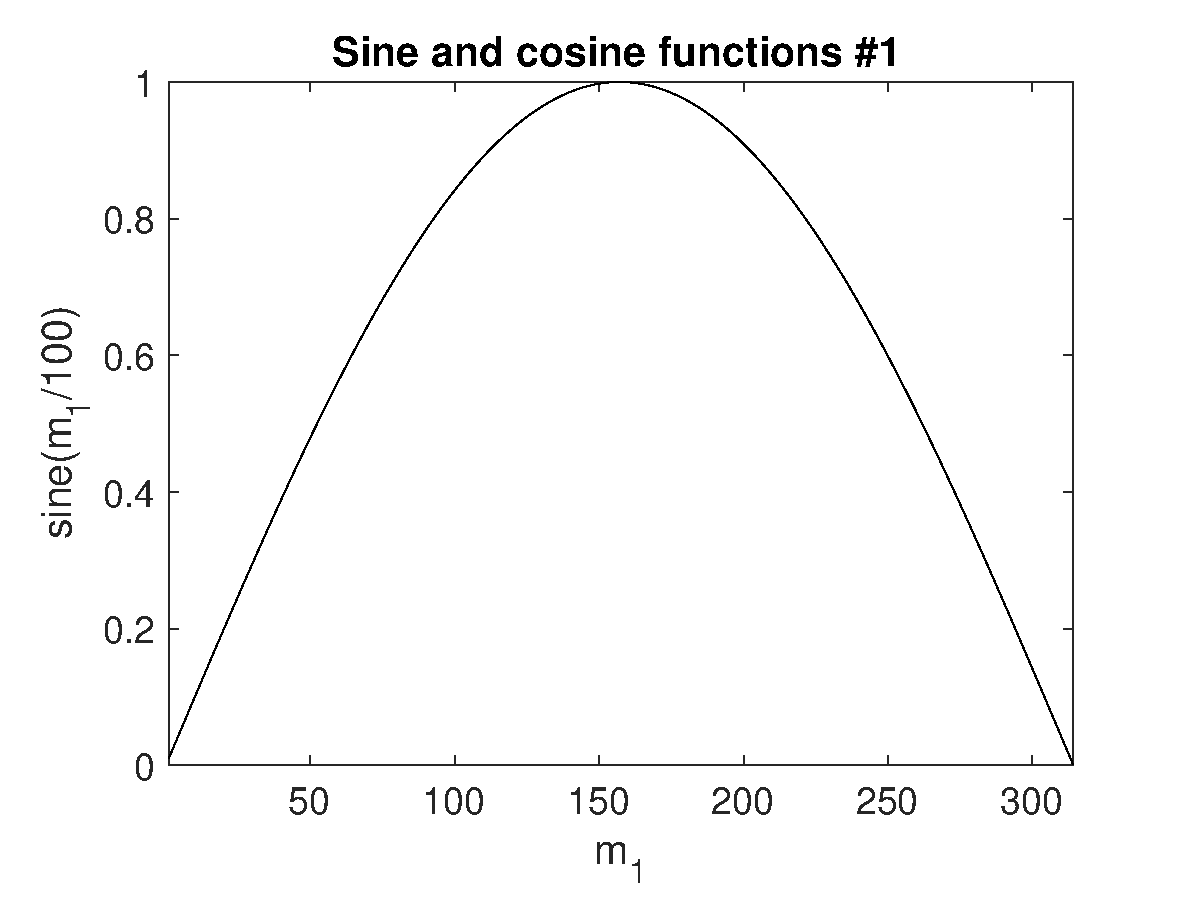
\includegraphics[width=0.5\textwidth]{xGraphfig1}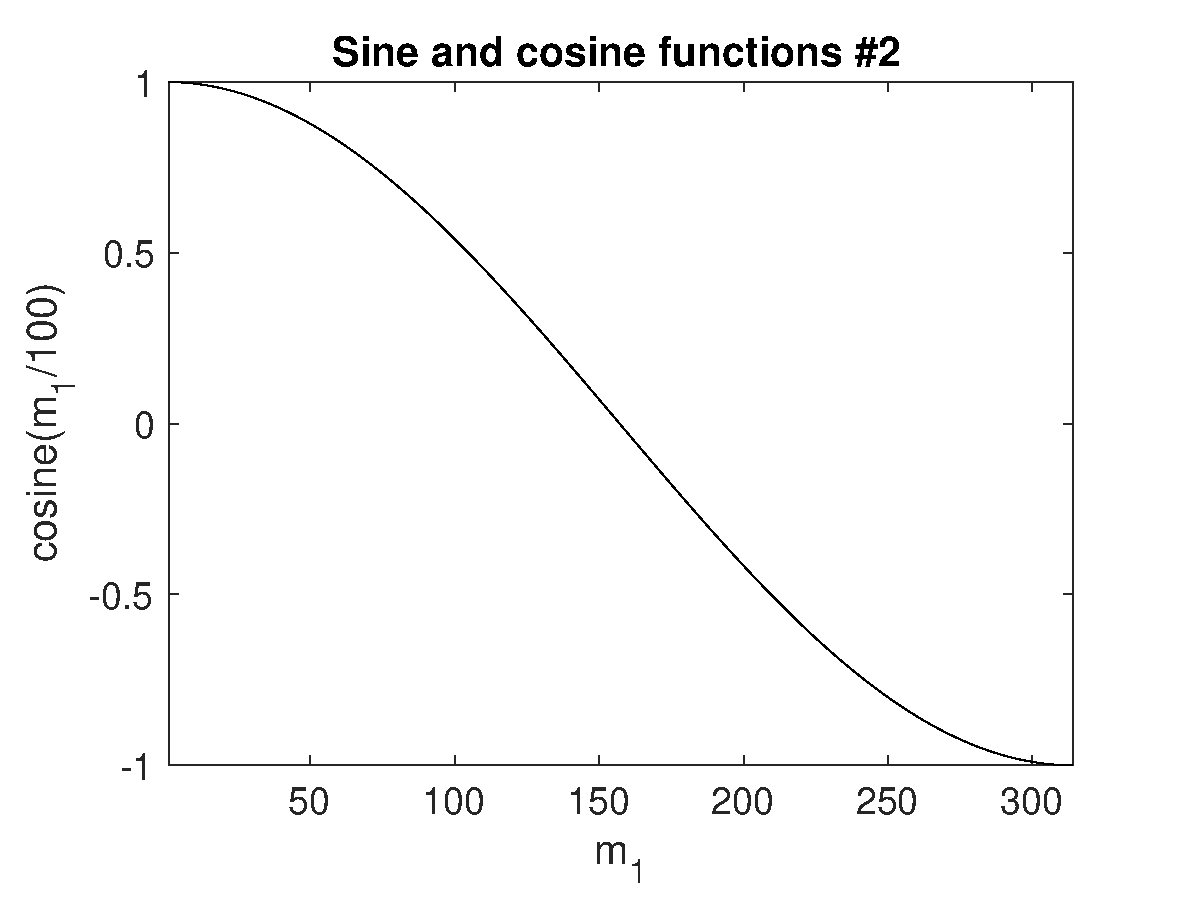
\includegraphics[width=0.5\textwidth]{xGraphfig2}

\caption{\emph{Example: xgraph output of two plots.}}
\vspace{10pt}
 
\end{figure}

Note that in this case the default setting of \emph{p.errors=0 }is
used, with no check index used in the data arrays, because these are
simple graphs without error-bars or comparisons.

\subsection{xGRAPH data arrays}

The data input to \emph{xGRAPH }can come from a file, or from data
generated directly from any compatible program.

The data is stored in a cell array $data$ with structure: 
\[
data\{s\}\{n\}(\ell,\mathbf{j},c)
\]
Each member of the outer cell array \emph{data\{s\}} defines a number
of related sets of graphical data, all described by common parameters
\emph{input\{s\}}. Comparisons and errors are plotted if there are
errors and comparison data in the input, indexed by \emph{c}. This
generates comparison plots, as well as error totals and $\chi$- squared
error estimate when there are statistical variances available.

An individual member of \emph{data\{s\}\{n\}} is a multidimensional
array, called a \emph{graph} in the xSPDE User's guide. For each \emph{graph},
multiple different plots with different dimensionality can be obtained
from the dataset \emph{data\{s\}\{n\}}, either through projections
and slices or by generating additional data defined with graphics
functions. Either or both alternatives are available.

Note that: 
\begin{itemize}
\item If a sequence has one member, the outer cell array can be omitted. 
\item In this simplified case, if there is only one \emph{graph} array,
the inner cell array can be omitted. 
\end{itemize}
The graphics data for a single dataset is held in a multidimensional
real array, where: 
\begin{itemize}
\item $\ell$ is the index for lines in the graph. Even for one line, the
first dimension is retained. 
\item $\mathbf{j}=j_{1},\ldots j_{d}$ is the array index in each dimension,
where $d\ge1$. 
\item Averages in momentum space have the momentum origin as the central
index. 
\item If integrals or spatial averages are used, the corresponding dimension
has one index $j_{d}=1$. 
\item With probabilities, extra dimensions are added to $\mathbf{j}$ to
store the bin indices. 
\item \emph{c} indexes error-checks and comparisons. If not present, omit
\emph{p.errors} and the last dimension. 
\item If $c>p.errors$, the extra fields are comparison inputs, where $p.errors$
is the largest data index. 
\end{itemize}
When the optional comparison fields are used, an input parameter $errors$
is required to indicate the maximum error index, to distinguish data
from comparisons. Parameter structures from xSIM have $errors=3$
set to allow for both sampling errors and discretization errors. If
this is omitted, the default is $errors=0$, which implies that there
is no error or comparison data

If $errors>0$, the last index can have larger values with $c>errors$,
for comparisons. The special case of $errors=1$ is used if the data
has no error bars, but there are comparisons in the data. Larger indices
are used to index the comparison data, which can also have two types
of errors. The largest usable last index is $errors+3$.

It is possible to directly plot the \emph{raw }data using xGRAPH.
One can even combine the raw data with a graphics parameter input.
But since the raw data has no error estimates - it is raw data - one
must set $p.errors=0$, since the xsim output parameters have a normal
setting of $p.errors=3$. This will give a single trajectory.

However, the raw data from a simulation typically includes many trajectories
if\emph{ $ensembles(1)>0$}. One must select particular trajectory
datasets from the raw cell array, to plot just one.

\subsection{Input parameters and defaults}

A sequence of graph parameters is obtained from inputs in a cell array,
as \emph{input = \{in1, in2, ...\}}. The input parameters of each
simulation in the sequence are specified in a Matlab structure. The
inputs are numbers, vectors, strings, functions and cell arrays. All
metadata has preferred values, so only changes from the preferences
need to be input. The resulting data is stored internally as a sequence
of structures in a cell array, to describe the simulation sequence.

The graphics parameters are also stored in the cell array \emph{input}
as a sequence of structures \emph{p.} This only need to be input when
the graphs are generated and can be changed at a later time to alter
the graphics output. A sequence of simulations is graphed from \emph{input}
specifications.

If there is one simulation, just one structure can be input, without
the sequence braces. The standard way to input each parameter value
is:

\[
p.label=parameter
\]

The standard way to input a function handle is:

\[
p.label=@function
\]

The inputs are scalar or vector parameters or function handles. Quantities
relating to graphed averages are cell arrays, indexed by the graph
number. The available inputs, with their default values in brackets,
are given below.

Simulation metadata, including default values that were used in a
particular simulation, can be included in the input data files. This
is done in both the \emph{.mat} and the \emph{.h5} output files generated
by xSIM, so the entire graphics input can be reconstructed or changed.

Parameters can be numbers, vectors, strings or cell arrays. Conventions
that are used are that: 
\begin{itemize}
\item All input parameters have default values 
\item Vector inputs of numbers are enclosed in square brackets, \emph{{[}...{]}}. 
\item Cell arrays of strings, functions or vectors are enclosed in curly
brackets. 
\item Vector or cell array inputs with only one member don’t require brackets. 
\item Incomplete parameter inputs are completed with the last used default
value. 
\item Function definitions can be handles pointing elsewhere, or defined
inline. 
\end{itemize}
If any inputs are omitted, there are default values which are set
by the internal function\emph{ xgpreferences}. The defaults can be
changed by editing \emph{xgpreferences}.

In the following descriptions, \emph{graphs} is the total number of
graphed variables of all types. The space coordinate, image, image-type
and transverse data can be omitted if there is no spatial lattice,
that is, if the dimension variable is set to one.

For uniformity, the graphics parameters that reference an individual
data object are cell arrays. These are indexed over the graph number
using braces \emph{\{\}}. If a different type of input is used, like
a scalar or matrix, xSPDE will attempt to convert the type to a cell
array.

Axis labels are cell arrays, indexed over dimension. The graph number
used to index these cell arrays refers to the data object. In each
case there can be multiple generated plots, depending on the graphics
input.

\subsection{Cascaded plots}

The xGRAPH function generates a default range of graphs, but this
can be modified to suit the user. In the simplest case of one dimension,
one graph dataset will generate a single plot. For higher dimensions,
a cascade of plots is generated to allow visualization, starting from
3D movies, then 3D static plots and finally 2D slices. These can also
be user modified.

Note that for all probabilities, the plot dimension is increased by
the bin range dimensionality.

\subsection{Plot dimensions}

The \emph{pdimension} input sets the maximum plotted dimensions. For
example, $pdimension\{1\}=1$ means that only plots vs $r_{1}$ are
output for the first function plotted. Default values are used for
the non-plotted dimensions, unless there are axes specified, as indicated
below.

The graphs cascade down from higher to lower dimensions, generating
different types of graphs. Each type of graph is generated once for
each function index.

\subsection{Plot axes}

The graphics axes that are used for plotting and the points plotted
are defined using the optional \emph{axes}\textbf{\emph{ }}input parameters,
where $axes\{n\}$ indicates the \emph{n}-th specified graph or set
of generated graph data.

If there are no \emph{axes}\textbf{\emph{ }}inputs, or the \emph{axes}
inputs are zero - for example, $axes\{1\}=\{0,0,0\}$ - only the lowest
dimensions are plotted, up to \emph{3}. If either the data or \emph{axes}\textbf{\emph{
}}inputs project one point in a given dimension, - for example, $axes\{1\}=\{0,31,-1,0\}$,
this dimension is suppressed in the plots, which reduces the effective
dimension of the data - in this case to two dimensions.

Examples: 
\begin{itemize}
\item $axes\{1\}=\{0\}$ - For function 1, plot all the first dimensional
points; higher dimensions get defaults. 
\item $axes\{2\}=\{-2,0\}$ - For function 2, plot the maximum value of
$r_{1}$ (the default) and all higher-dimensional x-points. 
\item $axes\{3\}=\{1:4:51,32,64\}$ - For function 3, plot every 4-th $x_{1}$
point at $x_{2}$ point 32, $x_{3}$ point 64 
\item $axes\{4\}=\{0,2:4:48,0\}$ - For function 4, plot every $x_{1}$
point , every 4-th $x_{2}$ point, and all $x_{3}$-points. 
\end{itemize}
Points labelled $-1$ indicates a default `typical' point, which is
the midpoint. If one uses $-2$, this is the last point.

Lower dimensions are replaced by corresponding higher dimensions if
there are \emph{dimensions} or \emph{axes} that are suppressed. Slices
can be taken at any desired point, not just the midpoint. The notation
of $axes\{1\}=\{6:3:81\}$, is used to modify the starting, interval,
and finishing points for complete control on the plot points.

The graphics results depend on the resulting \textbf{effective} dimension,
which is equal to the actual input data dimension unless there is
an \emph{axes} suppression, described above. Since the plot has to
include a data axis, the plot itself will usually have an extra data
axis.

One can plot only three axes directly using standard graphics tools.
The strategy to deal with the higher effective dimensionality is as
follows. For simplicity, ``time'' is used to label the first effective
dimension, although in fact any first dimension is possible: 
\begin{description}
\item [{\emph{dimensions~=~1}}] For one lattice dimension, a 2D plot
of observable\emph{ vs t} is plotted, with data at each lattice point
in time. Exact results, error bars and sampling error bounds are included
if available. 
\item [{\emph{dimensions~=~2}}] For two lattice dimensions, a 3D image
of observable\emph{ vs x,t} is plotted. A movie of distinct 2D graphic
plots is also possible. Otherwise, a slice through $x=0$ is used
tp reduce the lattice dimension to $1$. 
\item [{\emph{dimensions~=~3}}] For three lattice dimensions, if $images>1$,
a movie of distinct 3D graphic images of observables are plotted as
$images$ slices versus the first plot dimension. Otherwise, a slice
through the chosen point, is used at the highest dimension to reduce
the lattice dimension to $2$. 
\item [{\emph{dimensions~=~4,5..}}] For higher lattice dimensions, a
slice through a chosen point, or the default midpoint is used to reduce
the lattice dimension to $3$. 
\end{description}
As explained above, in addition to graphs versus $x_{1}$ the \textbf{xGRAPH}
function can generate \emph{images }(3D)\emph{ }and \emph{transverse}
(2D) plots at specified points, up to a maximum given by the number
of points specified. The number of these can be individually specified
for each graph number. The images available are specified as\emph{
imagetype}$=1,\ldots4$, giving: 
\begin{enumerate}
\item 3D perspective plots (Matlab \emph{surf} - the default) 
\item 2D filled color plots (Matlab \emph{contourf} ) 
\item contour plots (Matlab \emph{contour} ) 
\item pseudo-color plots (Matlab \emph{pcolor} ) 
\end{enumerate}
Error bars, sampling errors and multiple lines for comparisons are
only graphed for 2D plots. Error-bars are not plotted when they are
below a user-specified size, with a default of $1\%$ of the maximum
range, to improve graphics quality. Higher dimensional graphs do not
output error-bar data, but they are still recorded in the data files.

\subsection{Probabilities and parametric plots}

Probability data can be input and plotted like any other data. It
is typically generated from simulation programs using the $binranges$
data for binning. It is plotted like any other graph, with any dimension,
except that the total dimension is extended by the number of variables
or lines in the \emph{observe} function.

\subsection{Chi-squared plots}

In addition the program can make a\emph{ }$\chi^{2}$ plot, which
is a plot of the $\chi^{2}$ comparison with a comparison probability
density against space and/or time. This allows a test of the simulated
data against a known target probability distribution, provided that
the following input data conditions are satisfied: 
\begin{itemize}
\item The input data dimension exceeds the p.\emph{dimensions} parameter, 
\item The switch p.\emph{chisqplot }is set to $1$or 2, and 
\item The input data includes comparison function data. 
\end{itemize}
The\emph{ }$\chi^{2}$ plots, depending on $p.chisqplot$ are: 
\begin{enumerate}
\item a plot of $\chi^{2}$ and $k$, where $k$ is the number of valid
data points, 
\item a plot of $\sqrt{2\chi^{2}}$ and $\sqrt{2k-1}$, which should have
a unit variance. 
\end{enumerate}
Here, for one point in space and time, with $m$ bins, $N_{j}$ counts
per bin and $E_{j}$ expected counts: 
\begin{equation}
\chi^{2}=\sum_{j=1}^{m}\frac{\left(N_{j}-E_{j}\right)^{2}}{E_{j}}.
\end{equation}

The number $k$ is the number of valid counts, with $N_{j},E_{j}>mincount$.
This is partly determined from the requirement that the probability
count data per bin is greater than the $p.mincount$ parameter. The
default is set to give a number of samples $>10$. The program prints
a summary that sums over of all the $\chi^{2}$ data.

The $p.scale\{n\}$ parameter gives the number of counts per bin at
unit probability density. This is needed to set the scale of the $\chi^{2}$
results, ie, $N_{j}=scale\{n\}\times p_{j}$, where $p_{j}$ is the
probability density that is compared and plotted in the simulation
data. Note that a uniform bin size is assumed here, to give a uniform
scaling.

\subsection{Comparisons with variances}

It can be useful to compare two probability distributions with different
variances. For one point in space and time, with $m$ bins, $p_{j}$
probability density and $e_{j}$ expected probability density, 
\begin{equation}
\chi^{2}=\sum_{j=1}^{m}\frac{\left(p_{j}-e_{j}\right)^{2}}{\sigma_{j}^{2}+\sigma_{e,j}^{2}}.
\end{equation}
In this case, $\sigma_{j}^{2}$ and $\sigma_{e,j}^{2}$ are the sampling
errors in the simulation data and comparison data, so that built-in
error fields in the data are used to work out the $\chi^{2}$ results.
This option is chosen if $p.scale\{n\}=0$, and the cutoff for the
data is then specified so that $p_{j},e_{j}>p.cutoffs\{n\}$. This
only has a $\chi^{2}$ distribution if points are independent.

\subsection{Maximum likelihood}

It is also possible to plot the $G^{2}$ or maximum likelihood plot
of the data, which is an alternative means to compare distributions,
where 
\begin{equation}
G^{2}=2\sum_{j=1}^{m}N_{j}\ln\left(N_{j}/E_{j}\right).
\end{equation}
The expected values $E_{j}$ are automatically scaled so that $\sum N_{j}=\sum E_{j},$with
the same minimum count cutoff that is used for the $\chi^{2}$ data.
The result is similar to the $\chi^{2}$ results. It is obtained if
p.\emph{gsqplot }is set to $1$ or 2 and requires for the input that
$p.scale\{n\}>0.$ It is sometimes regarded as a preferred method
for comparisons.

\subsection{Parametric plots}

Any input dataset can be converted to a parametric plot, where a second
data input is plotted along the horizontal axis instead of the time
coordinate. It is also possible to substitute a second data input
for the x-axis data if a parametric plot in space is required instead.
This allows visualization of how one type of data changes as a function
of a second type of data input.

The two datasets that are plotted must have the same number of lines,
that is, the first index range should be the same, in order that multiple
lines can be compared. This is achieved where required using the \emph{p.scatters}
input in the simulation code. The details of the parametric plot are
specified using the input: \emph{ 
\begin{equation}
p.parametric\{n\}=[n1,p2]
\end{equation}
}

Here $n$ is the graph number which is plotted, and must correspond
to an input dataset. The number $n1$ is the graph number of the observable
that is plotted on the horizontal axis, ignoring functional transformations.
The second number is the axis number where the parametric value is
substituted, which can be the time (axis 1) or the x-coordinate (axis
2), if present.

In all cases the vertical axis is used to plot the original data.
The specified horizontal axis is used for the parametric variable.
Only vertical error-bars are available. An example is given in xAMPLES/SDE\_1/SHO,
which is a noise-driven harmonic oscillator, with several lines plotted
of $x$ vs \emph{y}.

\section{Parameter reference\label{sec:Parameter-reference}}

\subsection{\emph{axes\{n\}}}
\begin{description}
\item [{Default:}] \emph{\{0,0,0,..\}} 
\end{description}
Gives the axis points plotted for the $n$-th plotted function, in
each dimension. Each entry value is a vector range for a particular
plot and dimension. Thus, \emph{p = 5} gives the fifth point only,
and a vector input \emph{p = 1:4:41} plots every fourth point. Single
points generate graphics projections, allowing the other dimensions
to be plotted. Zero or negative values are shorthand. For example,
\emph{p = -1} generates a default point at the midpoint, \emph{p =
-2} the endpoint, and \emph{p = 0} is the default value that gives
the vector for the every axis point. For each graph type, i.e. \emph{n=1,..graphs}
the axes can be individually specified in each dimension, \emph{d=1,..dimension}s.
If more than three axes are specified to be vectors, only the first
three are used, and others are set to default values in the plots. 
\begin{description}
\item [{Example:}] \emph{p.axes\{4\} = \{1:2:10,0,0,-1\}} 
\end{description}

\subsection{\emph{diffplot\{n\}}}
\begin{description}
\item [{Default:}] \emph{0} 
\end{description}
Differences are plotted as a comparison dashed line on $2D$ plots
as a default. Otherwise, a separate difference plot is obtained which
is unnormalized (\emph{diffplot = 1)}, or normalized\emph{ }(\emph{diffplot
= 2) }by the total RMS errors. If \emph{diffplot = 3}, the comparison
data is plotted directly as an additional graph. 
\begin{description}
\item [{Example:}] \emph{p.diffplot\{3\} = 2} 
\end{description}

\subsection{\emph{errors}}
\begin{description}
\item [{Default:}] \emph{0} 
\end{description}
Indicates if the last index in the graphics input data arrays is used
for error-bars and/or comparisons. Should be set to zero if there
is no error or comparison data. If non-zero, this will give the highest
last index used for errors. The standard \emph{xsim} output sets \emph{$p.errors=3$
}automatically. As a special case, \emph{$p.errors=1$ }is used to
indicate that there is comparison data but no error data.

If \emph{$p.errors>0$ }, the data indexed up to \emph{p.errors} gives
the data, then a maximum of two types of error bars. Up to three further
index values, up to \emph{$p.errors+3$,} are available to index all
comparison data and its error fields. The maximum last index value
used is $6$. 
\begin{description}
\item [{Example:}] \emph{p.errors = 2} 
\end{description}

\subsection{\emph{esample\{n\}}}
\begin{description}
\item [{Default:}] \emph{1} 
\end{description}
This sets the type and size of sampling errors that are plotted. If
\emph{esample = 0}, no sampling error lines are plotted, just the
mean. If $esample=-n$, $\pm n\sigma$ sampling errors are included
in the error-bars. If $esample=n$, separate upper and lower $\pm n\sigma$
sampling error lines are plotted. In both cases, the magnitude of
esample sets the number of standard deviations used. 
\begin{description}
\item [{Example:}] \emph{p.esample\{3\} = -1} 
\end{description}

\subsection{\emph{font\{n\}}}
\begin{description}
\item [{Default:}] \emph{18} 
\end{description}
This sets the default font sizes for the graph labels, indexed by
graph. This can be changed per graph. 
\begin{description}
\item [{Example:}] \emph{p.font\{4\}=18} 
\end{description}

\subsection{\emph{functions}}
\begin{description}
\item [{Default:}] number of functional transformations 
\end{description}
This gives the maximum number of output graph functions and is available
to restrict graphical output. The default is the length of the cell
array of input data. Normally, the default will be used. 
\begin{description}
\item [{Example:}] \emph{p.functions = 10} 
\end{description}

\subsection{\emph{glabels\{n\}}}
\begin{description}
\item [{Default:}] \emph{xlabels} or \emph{klabels} 
\end{description}
Graph-dependent labels for the independent variable labels. This is
a nested cell array with first dimension of \emph{graphs} and second
dimension of \emph{dimension}s. This is used to replace the global
values of \emph{xlabels} or \emph{klabels} if the axis labels change
from graph to graph, for example, if the coordinates have a functional
transform. These can be set for an individual coordinate on one graph
if needed. 
\begin{description}
\item [{Example:}] \emph{p.glabels\{4\}\{2\} = 'x\textasciicircum 2'} 
\end{description}

\subsection{\emph{graphs}}
\begin{description}
\item [{Default:}] observables to plot 
\end{description}
This gives the observables to plot. The default is a vector of indices
from one to the length of the cell array of observe functions. Normally
not initialized, as the default is used. Mostly used to reduce graphical
output on a long file. 
\begin{description}
\item [{Example:}] \emph{p.graphs = 10} 
\end{description}

\subsection{\emph{gtransforms\{n\}}}
\begin{description}
\item [{Default:}] {[}0,0,...{]} 
\end{description}
This switch specifies the Fourier transformed graphs and axes for
graphics labeling. Automatically equal to \emph{ftransforms} if from
an earlier xSIM input, but can be changed. If altered for a given
graph, all the axis Fourier switches should be reset. This is ignored
if there is no \emph{dimensions} setting to indicate space dimensions. 
\begin{description}
\item [{Example:}] \emph{p.gtransforms\{1\} = {[}0,0,1{]}} 
\end{description}

\subsection{\emph{headers\{n\}}}
\begin{description}
\item [{Default:}] \emph{''} 
\end{description}
This is a string variable giving the graph headers for each type of
function plotted. The default value is an empty string. Otherwise,
the header string that is input is used. Either is combined with the
simulation name and a graph number to identify the graph. This is
used to include simulation headers to identify graphs in simulation
outputs. Graph headers may not be needed in a final published result.
For this, either edit the graph, or use a space to make plot headers
blank:\emph{ p.headers\{n\} = ' '}, or \emph{p.name = ' '} . 
\begin{description}
\item [{Example:}] \emph{p.headers\{n\} = 'my\_graph\_header'} 
\end{description}

\subsection{\emph{images\{n\}}}
\begin{description}
\item [{Default:}] \emph{0} 
\end{description}
This is the number of 3D, transverse o-x-y images plotted as discrete
time slices. Only valid if the input data dimension is greater than
2. If present, the coordinates not plotted are set to their central
value when plotting the transverse images. This input should have
a value from zero up to a maximum value of the number of plotted points.
It has a vector length equal to \emph{graphs.} 
\begin{description}
\item [{Example:}] \emph{p.images\{4\} = 5} 
\end{description}

\subsection{\emph{imagetype\{n\}}}
\begin{description}
\item [{Default:}] \emph{1} 
\end{description}
This is the type of transverse o-x-y movie images plotted. It has
a vector length equal to \emph{graphs}. 
\begin{itemize}
\item \emph{imagetype =} \emph{1 }gives a perspective surface plot 
\item \emph{imagetype =} \emph{2}, gives a 2D plot with colors 
\item \emph{imagetype =} 3 gives a contour plot with 10 equally spaced contours 
\item \emph{imagetype =} 4 gives a pseudo-color map 
\end{itemize}
\begin{description}
\item [{Example:}] \emph{p.imagetype\{n\} = 1, 2, 3, 4} 
\end{description}

\subsection{\emph{klabels}}
\begin{description}
\item [{Default:}] \emph{\{'\textbackslash omega', 'k\_x', 'k\_y', 'k\_z'\}``
or ``\{'k\_1', 'k\_2', 'k\_3', 'k\_4',...\}} 
\end{description}
Labels for the graph axis Fourier transform labels, vector length
of \emph{dimension}s. The numerical labeling default is used when
the ``\emph{p.numberaxis}`` option is set. Note, these are typeset
in Latex mathematics mode! When changing from the default values,
all the required new labels must be set. 
\begin{description}
\item [{Example:}] \emph{p.klabels= \{'\textbackslash Omega', 'K\_x',
'K\_y',\}} 
\end{description}

\subsection{\emph{legends\{n\}}}
\begin{description}
\item [{Default:}] \emph{\{'',''\}} 
\end{description}
Graph-dependent legends, specified as a nested cell array of strings
for each line. 
\begin{description}
\item [{Example:}] \emph{p.legends\{n\} = \{labels(1), ..., labels(lines)\}} 
\end{description}

\subsection{\emph{limits\{n\}}}
\begin{description}
\item [{Default:}] \emph{\{0,0,0,0; ...\}} 
\end{description}
Graph-dependent limits specified as a cell array with dimension \emph{graphs}.
Each entry is a cell array of graph limits indexed by the dimension,
starting from $d=1$ for the time dimension. The limits are vectors,
indexed as 1,2 for the lower and upper plot limits. This is useful
if the limits required change from graph to graph. If an automatic
limit is required for either the upper or lower limit, it is set to
\emph{inf. }

An invalid, scalar or empty limit vector, like {[}0,0{]} or $0$ or
{[}{]} is ignored, and an automatic graph limit is used. 
\begin{description}
\item [{Example:}] \emph{p.limits\{n\} = \{{[}t1,t2{]},{[}x1,x2{]},{[}y1,y2{]}
...,\}} 
\end{description}

\subsection{\emph{linestyle\{n\}}}
\begin{description}
\item [{Default:}] \emph{\{'-k','-{}-k',':k','-.k','-ok','-{}-ok',':ok','-.ok','-+k','-{}-+k'\}} 
\end{description}
Line types for each line in every two-dimensional graph plotted. If
a given line on a two-dimensional line is to be removed completely,
set the relevant line-style to zero. For example, to remove the first
line from graph 3, set p.linestyle\{3\} =\{0\}. This is useful when
generating and changing graphics output from a saved data file. The
linestyle uses Matlab terminology. It allows setting the line pattern,
marker symbols and color for every line. The default lines are black
(\emph{'k'}), but any other color can be used instead.

The specifiers must be chosen from the list below, eg, '-ok', although
the marker can be omitted if not required. 
\begin{itemize}
\item Line patterns: '-' (solid), '--' (dashed), ':' (dotted) ,'-.' (dash-dot) 
\item Marker symbols: '+','o','{*}','.','x','s','d','\textasciicircum ','v','\textgreater
','\textless ','p' 
\item Colors: 'r','g','b','c','m','y','k','w' 
\end{itemize}
\begin{description}
\item [{Example:}] \emph{p.linestyle\{4\} = \{'-k','-{}-ok',':g','-.b',\}} 
\end{description}

\subsection{\emph{linewidth\{n\}}}
\begin{description}
\item [{Default:}] 0.5 
\end{description}
Line width for plotted lines in two-dimensional graphs. For example,
to make the lines wider in graph 3, set p.linewidth\{3\} =1. This
is useful for changing graphics output appearance if the default lines
are too thin. 
\begin{description}
\item [{Example:}] \emph{p.linewidth\{n\} = 1} 
\end{description}

\subsection{\emph{minbar\{n\}}}
\begin{description}
\item [{Default:}] \emph{\{0.01, ...\}} 
\end{description}
This is the minimum relative error-bar that is plotted. Set to a large
value to suppress unwanted error-bars, although its best not to ignore
the error-bar information! This can be changed per graph. 
\begin{description}
\item [{Example:}] \emph{p.minbar\{n\} = 0} 
\end{description}

\subsection{\emph{name}}
\begin{description}
\item [{Default:}] '' 
\end{description}
Name used to label simulation graphs, usually corresponding to the
equation or problem solved. This can be removed from individual graphs
by using \emph{headers\{n\}} equal to a single blank space. The default
is a null string. To remove all headers globally, set \emph{name}
equal to a single blank space: \emph{name = ' '.} 
\begin{description}
\item [{Example:}] \emph{p.name = 'Wiener process simulation'} 
\end{description}

\subsection{\emph{olabels\{n\}}}
\begin{description}
\item [{Default:}] \emph{'a'} 
\end{description}
Cell array of labels for the graph axis observables and functions.
These are text labels that are used on the graph axes. The default
value is \emph{'a\_1}' if the default observable is used, otherwise
it is blank. This is overwritten by any subsequent label input when
the graphics program is run: 
\begin{description}
\item [{Example:}] \emph{p.olabels\{4\} = 'v'} 
\end{description}

\subsection{\emph{parametric\{n\}}}
\begin{description}
\item [{Default:}] \emph{{[}0,0{]}} 
\end{description}
Cell array that defines parametric plots, for each graph number. The
first number is the graph number of the alternative observable plotted
on the horizontal axis. The second number is the axis number where
the parametric value is substituted, which can be the time (axis 1)
or the x-coordinate (axis 2), if present.

If both are zero, the plot against an independent space-time coordinate
is calculated as usual. If nonzero, a parametric plot is made for
two-dimensional plots. In all cases the vertical axis is used to plot
the original data. The specified horizontal axis is used for the parametric
variable. Only vertical error-bars are available. Can be usefully
combined with \emph{scatters\{n\}} to plot individual trajectories,
but the number of scatters should be the same in each of the two graphs
that are parametrically plotted against each other. 
\begin{description}
\item [{Example:}] \emph{p.parametric\{n\} = {[}p1,p2{]} \textgreater
= 0} 
\end{description}

\subsection{\label{subsec:pdimension}\emph{pdimension\{n\}}}
\begin{description}
\item [{Default:}] \emph{3} 
\end{description}
This is the maximum plotted space-time dimension for each plotted
quantity. The purpose is eliminate unwanted graphs. For example, it
is useful to reduce the maximum dimension when averaging in space.
Higher dimensional graphs are not needed, as the data is duplicated.
Averaging can be useful for checking conservation laws, or for averaging
over homogeneous data to reduce sampling errors. All graphs are suppressed
if it is set to zero. Any three dimensions can be chosen to be plotted,
using the \emph{axes} parameter to suppress the unwanted data points
in other dimensions. 
\begin{description}
\item [{Example:}] \emph{p.pdimension\{4\} = 2} 
\end{description}

\subsection{\emph{saveeps}}
\begin{description}
\item [{Default:}] 0 
\end{description}
If set to $1$, all plots are saved to the current folder as .eps
files, numbered consecutively. It is best to use the \emph{close all}
command first to remove unwanted displayed xFIGURES, before running
\emph{xgraph} with this option. 
\begin{description}
\item [{Example:}] \emph{p.saveeps =1} 
\end{description}

\subsection{\emph{savefig}}
\begin{description}
\item [{Default:}] 0 
\end{description}
If set to $1$, all plots are saved to the current folder as .fig
files, numbered consecutively. It is best to use the \emph{close all}
command first to remove unwanted displayed xFIGURES, before running
\emph{xgraph} with this option. 
\begin{description}
\item [{Example:}] \emph{p.savefig =1} 
\end{description}

\subsection{\emph{transverse\{n\}}}
\begin{description}
\item [{Default:}] \emph{0} 
\end{description}
This is the number of 2D transverse images plotted as discrete time
slices. Only valid if \emph{dimensions} is greater than 2. If present,
the $y,z$-coordinates are set to their central values when plotting
transverse images. Each element can be from 0 up to the number of
plotted time-points. The cell array has a vector length equal to \emph{graphs}. 
\begin{description}
\item [{Example:}] \emph{p.transverse\{n\}= 6} 
\end{description}

\subsection{\emph{verbose}}
\begin{description}
\item [{Default:}] 0 
\end{description}
Print flag for output information while running xGRAPH. Print options
are: 
\begin{itemize}
\item Minimal if \emph{verbose = -1}: Prints just the start-up time and
hard error messages 
\item Brief if \emph{verbose = 0}: Additionally prints the final, total
chi-squared errors where present 
\item Informative if \emph{verbose = 1}: Also prints the graph progress
indicators 
\item Full if \emph{verbose = 2}: Prints everything including the internal
parameter structure data. 
\end{itemize}
In summary, if \emph{verbose = 0}, most output is suppressed except
the final data, \emph{verbose = 1} displays a progress report, and
\emph{verbose = 2} additionally generates a readable summary of the
graphics parameter input. 
\begin{description}
\item [{Example:}] \emph{p.verbose = 0} 
\end{description}

\subsection{\emph{xlabels}}
\begin{description}
\item [{Default:}] \emph{\{'t', 'x', 'y', 'z'\}} or \{\emph{'x\_1', 'x\_2',
'x\_3', 'x\_4'},...\} 
\end{description}
Global labels for the independent variable labels, vector length equal
to \emph{dimension}s. The numerical labeling default is used when
the \emph{numberaxis} option is true. These are typeset in Latex mathematics
mode. When changing from the default values, all the required new
labels must be set. 
\begin{description}
\item [{Example:}] \emph{p.xlabels = \{'tau'\}} 
\end{description}

\subsection{\emph{gfunction\{n\} (d,p)}}

This is a cell array of graphics function handles. Use when a graph
is needed that is a functional transformation of the observed averages.
The default value generates the \emph{n-th }graph \emph{data} array
directly from the \emph{n-th }input \emph{data}. The input is the
data cell array for all the graphs in the current sequence number
with their graph parameters \emph{x}, and the output is the \emph{n-th
}data array that is plotted.

An arbitrary number of functions of these observables can be plotted,
including vector observables. The input to graphics functions is the
observed data averages or functions of averages in a given sequence,
each stored in a cell array $d\{n\}(\ell,\mathbf{j},c)$. If there
are more graphics functions than input data cells, this generate additional
data for plotting.

\subsection{\emph{xfunctions\{n\} \{nd\} (ax,p)}}

This is a nested cell array of axis transformations. Use when a graph
is needed with an axis that is a function of the original axes. The
input is the original axis coordinates, and the output is the new
coordinate set. The default value generates the input axes. Called
as \emph{xfunctions\{n\}\{nd\}(ax,p)} for the \emph{n}-th graph and
axis direction \emph{dir}, where \emph{ax} is a vector of coordinates
for that axis.There is one graphics function for each separate graph
dimension or axis. The default value is the coordinate vector $xk\{nd\}$
stored in the input parameter structure p, or else the relevant index
if \emph{xk\{nd\}} is omitted.

\section{xGRAPH structure}

The graphics function, $xgraph$, plots the simulation data. The general
structure is:

\begin{align*}
\mathbf{xgraph} & \rightarrow\mathbf{xgpreferences}\,\,(checks\,inputs)\\
 & \rightarrow\mathbf{xmultigraph}\leftrightarrow\mathbf{xreduce\leftrightarrow\mathbf{xcompress}}\,\,(structures\,data\,arrays)\\
 & \rightarrow\mathbf{ximages}\rightarrow\mathbf{xtransverse}\rightarrow\mathbf{xplot3}\rightarrow\mathbf{xplot2}\,\,(graphs\,all\,data)
\end{align*}

Most graphics functions simply work, but two important functions are
listed here for reference.

\subsection{\emph{xgraph(data,input)}}

The\emph{ xgraph} function graphs multidimensional data files. 
\begin{itemize}
\item Input: graphics data cells \emph{data}, input parameter cells \emph{input}. 
\item Output: graphs, displayed and/or stored as \emph{eps} or \emph{fig}
files. 
\item If no numeric \emph{data} present, reads data from a file named \emph{data}. 
\item If \emph{data} is present but without any \emph{input} parameters
it plots using default parameters. 
\item First data dimension is the line index, last dimension are the error-bars
and comparisons 
\item Needs: x\emph{read, xmakecell, xgpreferences, xmultiplot} 
\end{itemize}

\subsection{\emph{input = xgpreferences (input,oldinput)}}

The \emph{xgpreferences} function sets default values for graphics
inputs. 
\begin{itemize}
\item Input: \emph{input} cell array and optionally previous inputs from
a datafile, \emph{oldinput}. 
\item Note that each cell array is a sequence of graphics parameter structures 
\item Output: the updated plus default graphics parameters 
\item Called by: \emph{xgraph} 
\item Needs: \emph{xprefer}, \emph{xcprefer} 
\end{itemize}
\newpage{}

\chapter{Examples and batch testing\label{sec:Examples}}

A variety of examples are given in the xAMPLES folder distributed
with xSPDE. These can all be run using \emph{Batchtest.m}, which has
a typical runtime of $50-100s$, and runs $35$ different case studies.
This shows your distribution is intact. All the graphs produced are
deleted. It lists the different examples available, some of which
are given below.

The batch testing code will run each different example sequentially.
It prints the RMS relative errors for the step-size, sampling and
difference error, as well as the total RMS error combining all three,
the chi-square error normalised by the number of points, and the timing.
The geometric mean of the $35$ RMS total errors is computed as a
benchmark.

As Matlab random noise is reproducible with a fixed seed, this geometric
mean error is fixed. The total is printed to more than six decimals
for verification, and an error is indicated if it varies by a factor
of more than $\pm10^{-3}$. Due to different random noise algorithms
used in some Octave versions, the Octave error may vary by up to $\pm20\%$.

\section{SDE examples}

\subsection{Kubo}

This solves a multiplicative SDE with initial condition $a\left(0\right)=1$
and:

\begin{equation}
\frac{\partial a}{\partial t}=iaw(t)\,.\label{eq:SDE-3}
\end{equation}

The function uses the RK4 algorithm together with both vector and
series ensembles, then stores the computed averages with a comparison
of the variance and an exact solution, 
\begin{equation}
\left\langle a^{n}\right\rangle =e^{-tn^{2}/2}.
\end{equation}

\begin{center}
\doublebox{\begin{minipage}[t]{0.9\columnwidth}%
\texttt{function {[}e{]} = Kubo()}

\texttt{p.name = 'Kubo oscillator';}

\texttt{p.ensembles = {[}1000,8{]};}

\texttt{p.method = @RK4;}

\texttt{p.initial = @(w,p) 1;}

\texttt{p.deriv = @(a,w,p) 1i{*}w.{*}a(1,:) ;}

\texttt{p.file = 'Kubo.mat';}

\texttt{p.observe\{2\} = @(a,p) a.\textasciicircum 2;}

\texttt{p.olabels\{2\} = \{'\textless a\textasciicircum 2\textgreater
'\};}

\texttt{p.compare = \{@(p) exp(-p.t/2),@(p) exp(-2{*}p.t)\};}

\texttt{e = xsim(p);}

\texttt{p2.name = 'Kubo oscillator edited title';}

\texttt{xgraph(p.file,p2);}

\texttt{end}%
\end{minipage}} 
\par\end{center}

\paragraph{Notes}
\begin{itemize}
\item The algorithm is changed from the default to RK4. 
\item The data is stored to 'Kubo.mat'. 
\item This is re-read and edited using a second parameter structure, p2. 
\end{itemize}
\begin{figure}[H]
\centering{}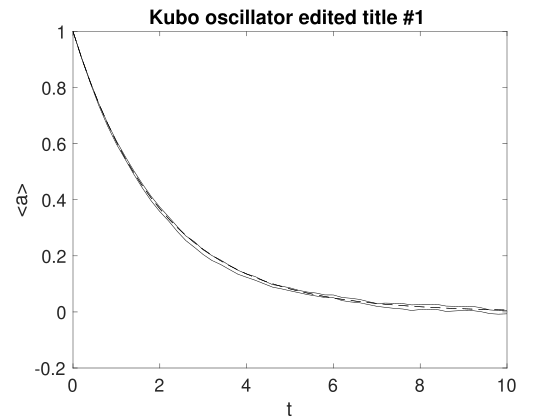
\includegraphics[width=0.75\textwidth]{Kubo-example1}\\
 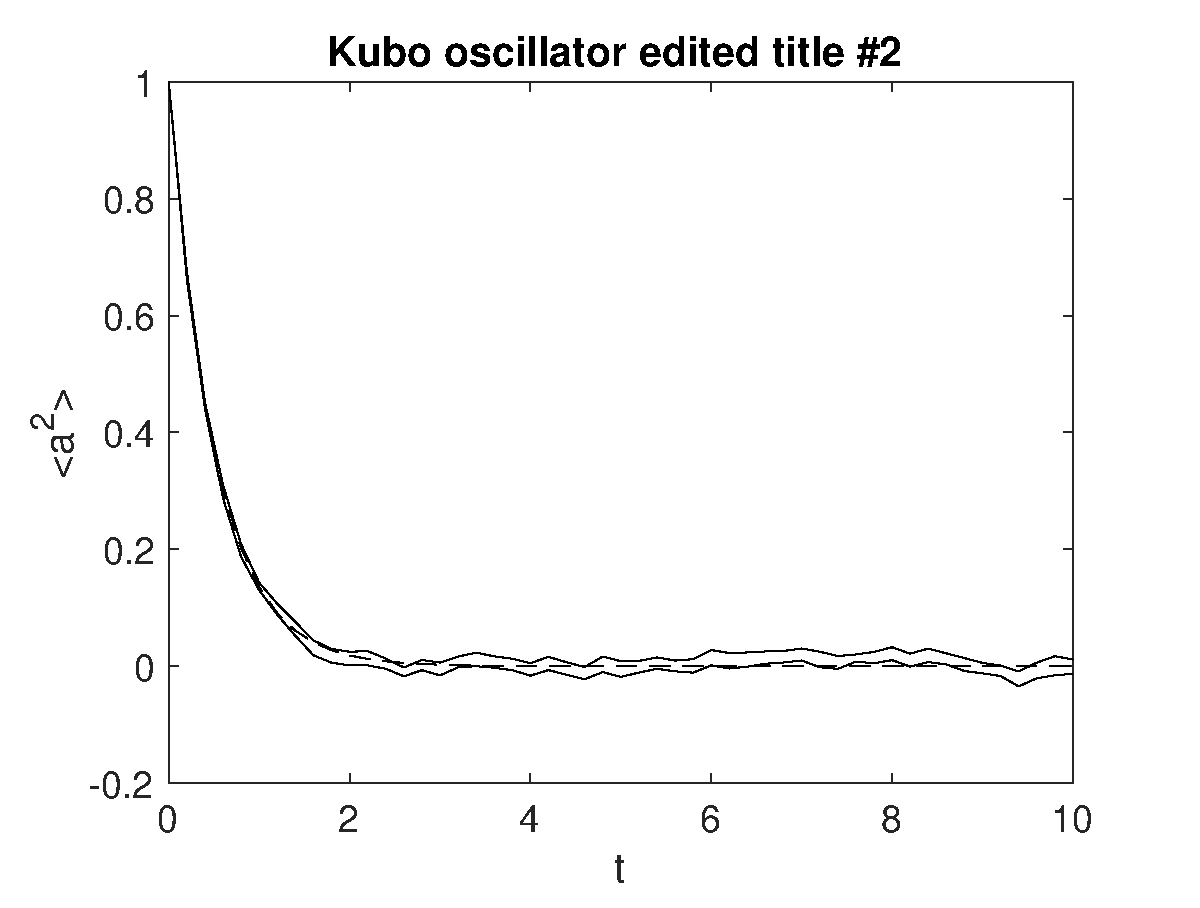
\includegraphics[width=0.75\textwidth]{Kubo-example2}

\caption{\emph{Example: Kubo oscillator. The graph shows the sampling error-bars
as two parallel lines. The discretization error-bars are less than
the minimum, and are not shown.}}
\vspace{10pt}
 
\end{figure}

\newpage{}

\subsection{Loss/Gain with noise}

This solves an SDE with a complex Gaussian distributed initial condition
having $\left\langle \left|a\left(0\right)\right|^{2}\right\rangle =1$
and a sequence of SDE equations, such that 
\begin{equation}
\frac{\partial a}{\partial t}=\begin{cases}
-a+w_{1}(t)+iw_{2}(t) & 0<t<4\\
a+w_{1}(t)+iw_{2}(t) & 4<t<8
\end{cases}\,.\label{eq:SDE-3-1-1}
\end{equation}

The computed variance is compared with an exact solution, 
\begin{equation}
\left\langle a^{2}\right\rangle =\begin{cases}
1 & 0<t<4\\
2e^{2\left(t-4\right)t}-1 & 4<t<8
\end{cases}.
\end{equation}

. 
\begin{center}
\doublebox{\begin{minipage}[t]{0.9\columnwidth}%
\texttt{function {[}e{]} = Gain()}

\texttt{p.name = 'Loss with noise';}

\texttt{p.ranges = 4;}

\texttt{p.noises = {[}2,0{]};}

\texttt{p.ensembles = {[}10000,1,10{]};}

\texttt{p.initial = @(w,\textasciitilde ) (w(1,:)+1i{*}w(2,:))/sqrt(2);}

\texttt{p.deriv = @(a,w,p) -a + w(1,:)+1i{*}w(2,:);}

\texttt{p.observe = \{@(a,\textasciitilde ) a.{*}conj(a)\};}

\texttt{p.olabels = \{'\textbar a\textbar\textasciicircum 2'\};}

\texttt{p.compare = \{@(p) 1\};}

\texttt{p2 = p;}

\texttt{p2.steps = 2;}

\texttt{p2.name = 'Gain with noise';}

\texttt{p2.deriv = @(a,w,\textasciitilde ) a + w(1,:)+1i{*}w(2,:);}

\texttt{p2.compare = \{@(p) 2{*}exp(2{*}(p.t-4))-1\};}

\texttt{e = xspde(\{p,p2\});}

\texttt{end}%
\end{minipage}} 
\par\end{center}

\paragraph{Notes}
\begin{itemize}
\item Low and high level parallel ensembles optimize use of multi-core vector
hardware. 
\item Two distinct simulations are run in series, with a change in the equation. 
\item The simulation name is changed in sequence 2, to distinguish the graphical
outputs 
\end{itemize}
\begin{figure}[H]
\centering{}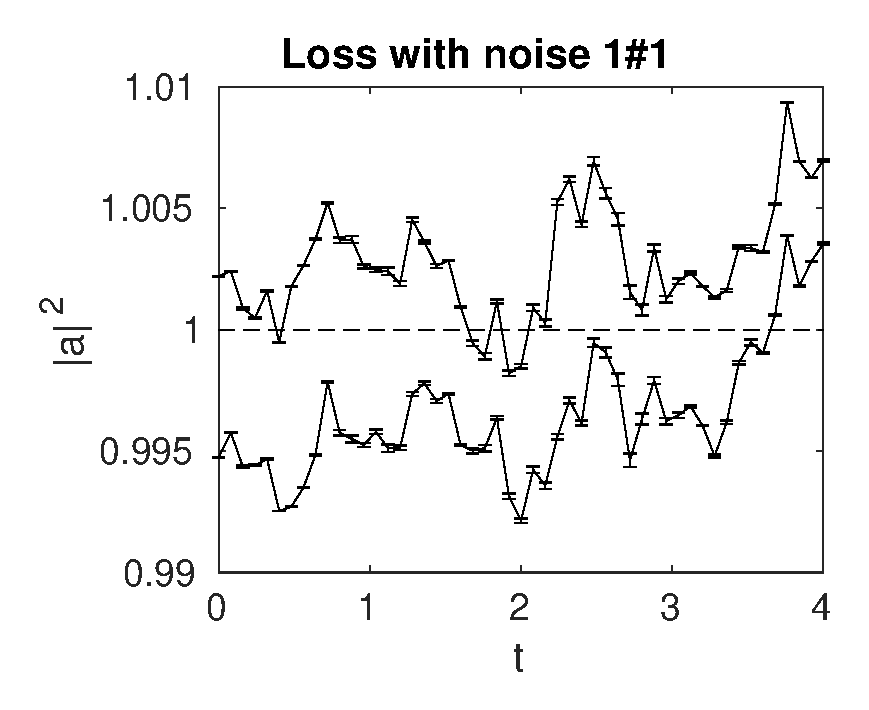
\includegraphics[width=0.75\textwidth]{Gain-example1}\\
 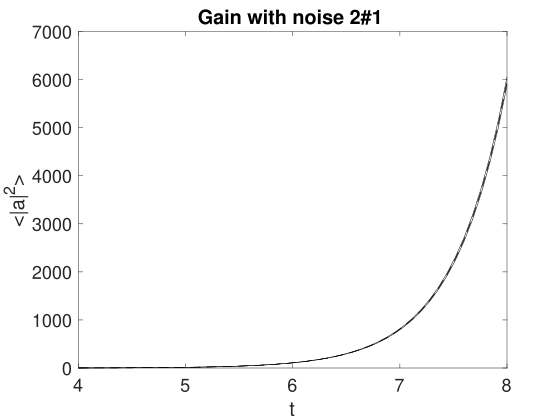
\includegraphics[width=0.75\textwidth]{Gain-example2}

\caption{\emph{Top figure: amplitude squared with loss balanced by noise. Bottom
figure, amplitude squared with gain. Graphs show excellent agreement
with theory up to the sampling errors of less than $\pm0.005$ in
the initial phase, shown by the parallel lines, with step errors of
order $\pm0.001$ indicated by error-bars.}}
\vspace{10pt}
 
\end{figure}

\pagebreak{}

\section{Spectral examples}

\subsection{Equilibrium}

This solves an SDE with a complex Gaussian initial condition having
$\left\langle \left|a\left(0\right)\right|^{2}\right\rangle =1$ and:

\begin{equation}
\frac{\partial a}{\partial t}=-a+w_{1}(t)+iw_{2}(t)\,.\label{eq:SDE-3-1}
\end{equation}

The equation is such that the initial distribution is also the equilibrium
probability distribution. The computed ordinary and spectral variances
are compared with exact solutions and graphed, where 
\begin{align}
\lim_{t\rightarrow\infty}\left\langle \left|a\left(t\right)\right|^{2}\right\rangle  & =1.\nonumber \\
\left\langle \left|a\left(\omega\right)\right|^{2}\right\rangle  & =\frac{T}{\pi\left(1+\omega^{2}\right)}.
\end{align}

\begin{center}
\doublebox{\begin{minipage}[t]{0.9\columnwidth}%
\texttt{function {[}e{]} = Equilibrium()}

\texttt{p.name = 'Equilibrium spectrum';}

\texttt{p.points = 101;}

\texttt{p.ranges = 100;}

\texttt{p.seed = 241;}

\texttt{p.noises = {[}2,0{]};}

\texttt{p.ensembles = {[}100,5{]};}

\texttt{p.initial = @(w,\textasciitilde ) (w(1,:)+1i{*}w(2,:))/sqrt(2);}

\texttt{p.deriv = @(a,w,\textasciitilde ) -a + w(1,:)+1i{*}w(2,:);}

\texttt{p.observe\{1\} = @(a,\textasciitilde ) a.{*}conj(a);}

\texttt{p.observe\{2\} = @(a,\textasciitilde ) a.{*}conj(a);}

\texttt{p.transforms = \{0,1\};}

\texttt{p.olabels = \{'\textbar a(t)\textbar\textasciicircum 2','\textbar
a(\textbackslash omega)\textbar\textasciicircum 2'\};}

\texttt{p.compare = \{@(p) 1, @(p)p.ranges(1)./(pi{*}(1+p.w.\textasciicircum 2))\};}

\texttt{e = xspde(p);}

\texttt{end}%
\end{minipage}} 
\par\end{center}

\paragraph{Notes}
\begin{itemize}
\item A fixed random seed is input using the \emph{p.seed} parameter. 
\item The \emph{p.transforms} cell array gives a Fourier transform for \emph{p.observe\{2\}}
only. 
\item A small number of ensembles and time-steps is used to improve error
visibility. 
\end{itemize}
\begin{figure}[H]
\centering{}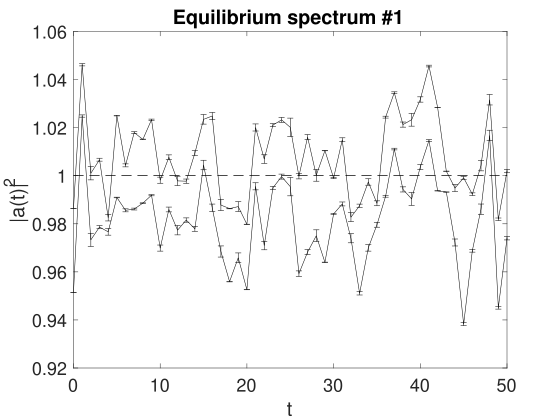
\includegraphics[width=0.75\textwidth]{Equilibrium-example1}\\
 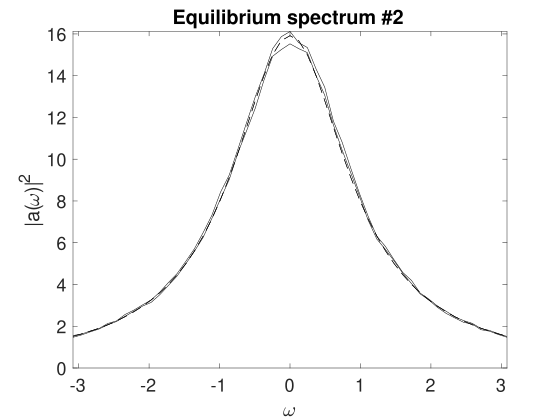
\includegraphics[width=0.75\textwidth]{Equilibrium-example2}

\caption{\emph{Top figure: Mean amplitude squared, showing invariant behavior
with time, apart from sampling errors. Bottom figure: Mean spectrum
as a function of frequency. The dashed lines are exact results, solid
lines are upper and lower sampling error bounds $(\pm\sigma)$, from
sampling the stochastic equations, the error-bars are errors due to
the step-size. Error bars are less than the minimum size for graphics
display in the bottom figure.}}
\vspace{10pt}
 
\end{figure}

\pagebreak{}

\subsection{Quantum}

This solves an SDE for a quantum harmonic oscillator in the (truncated)
Wigner phase-space calculus. It is initialized as a vacuum state,
corresponding to a complex Gaussian initial condition having $\left\langle \left|a\left(0\right)\right|^{2}\right\rangle =1$.
It is subject to vacuum noise, here realized by the auxiliary field
$a_{in}$. An output field is given through the input-output relations
and is realized by the auxiliary field $a_{out}$.

\begin{align}
\frac{\partial a}{\partial t} & =-a+\sqrt{2}a_{in}.\nonumber \\
a_{in} & =\frac{1}{2}\left(w_{1}(t)+iw_{2}(t)\,\right)\nonumber \\
a_{out} & =\sqrt{2}a-a_{in}
\end{align}

The computed spectral variances are compared with exact solutions
and graphed, where: 
\begin{align}
\frac{2\pi}{T}\left\langle \left|a\left(\omega\right)\right|^{2}\right\rangle  & =\frac{1}{\left(1+\omega^{2}\right)}.\nonumber \\
\left\langle \left|a_{in}\left(\omega\right)\right|^{2}\right\rangle  & =\frac{1}{2}\nonumber \\
\left\langle \left|a_{out}\left(\omega\right)\right|^{2}\right\rangle  & =\frac{1}{2}.
\end{align}


\paragraph{Notes}
\begin{itemize}
\item Demonstrates how to include defined fields 
\item There are $4$ steps per point, to give better accuracy due to finite
steps 
\item The observe functions are all transformed, and include defined fields. 
\end{itemize}
\begin{center}
\doublebox{\begin{minipage}[t]{0.9\columnwidth}%
\texttt{function e = Quantum()}

\texttt{p.name = 'Quantum harmonic oscillator spectrum';}

\texttt{p.points = 160;}

\texttt{p.steps = 4;}

\texttt{p.ranges = 120;}

\texttt{p.fields = 1;}

\texttt{p.auxfields = 2;}

\texttt{p.noises = 2;}

\texttt{p.ensembles = {[}400,1,12{]};}

\texttt{p.initial = @(w,\textasciitilde ) (w(1,:)+1i{*}w(2,:))/(2);}

\texttt{p.a1 = @(w) (w(1,:)+1i{*}w(2,:))/2;}

\texttt{p.deriv = @(a,w,\textasciitilde ) -a(1,:)+sqrt(2){*}p.a1(w);}

\texttt{p.define = @(a,w,p) {[}p.a1(w);sqrt(2){*}a(1,:)-p.a1(w){]};}

\texttt{T = @(p) p.ranges(1);}

\texttt{p.observe\{1\} = @(a,p) (2.{*}pi/T(p)){*}a(1,:).{*}conj(a(1,:));}

\texttt{p.observe\{2\} = @(a,p) (2.{*}pi/T(p)){*}a(2,:).{*}conj(a(2,:));}

\texttt{p.observe\{3\} = @(a,p) (2.{*}pi/T(p)){*}a(3,:).{*}conj(a(3,:));}

\texttt{p.transforms = \{1,1,1\};}

\texttt{p.olabels\{1\} = '\textbar a(\textbackslash omega)\textbar\textasciicircum 2';}

\texttt{p.olabels\{2\} = '\textbar a\_\{in\}(\textbackslash omega)\textbar\textasciicircum 2';}

\texttt{p.olabels\{3\} = '\textbar a\_\{out\}(\textbackslash omega)\textbar\textasciicircum 2';}

\texttt{p.compare\{1\} = @(p) 1./(1+p.w.\textasciicircum 2);}

\texttt{p.compare\{2\} = @(p) 0.5;}

\texttt{p.compare\{3\} = @(p) 0.5;}

\texttt{e = xspde(p);}

\texttt{end}%
\end{minipage}} 
\par\end{center}

\begin{figure}[H]
\begin{centering}
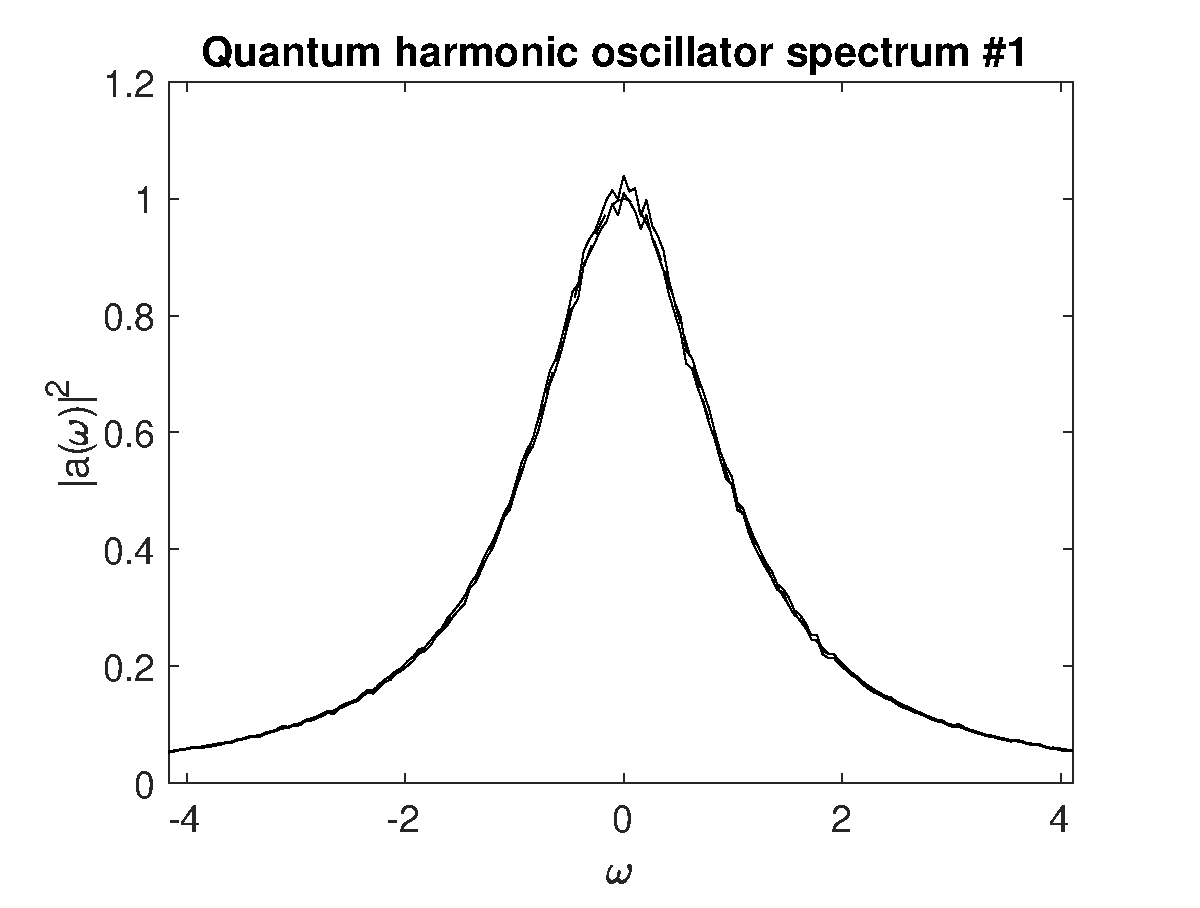
\includegraphics[width=0.75\textwidth]{Quantum-example1} 
\par\end{centering}
\centering{}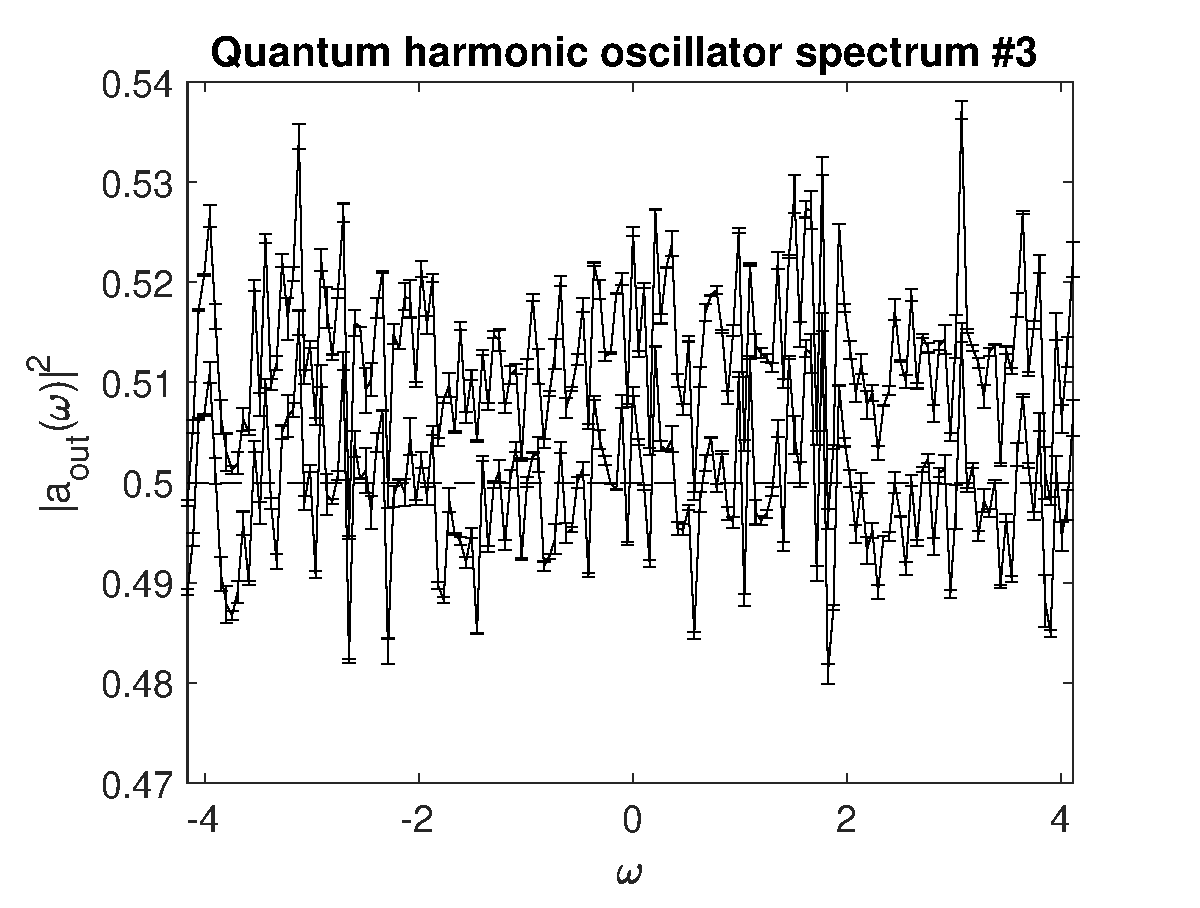
\includegraphics[width=0.75\textwidth]{Quantum-example2}

\caption{\emph{Top figure: Spectral density of the quantum state. Bottom figure:
Spectral density of the output field. The solid lines indicate upper
and lower sampling error bounds $(\pm\sigma)$, from sampling the
stochastic equations. The dashed lines are exact results, the error-bars
indicate step-size errors. Error bars are less than the minimum size
for display in the top figure.}}
\vspace{10pt}
 
\end{figure}

\pagebreak{}

\section{Probability examples}

\subsection{Probability density, Wiener process}

Solves an SDE with an initial condition $\left\langle a\left(0\right)\right\rangle ^{2}=\frac{1}{4}$
and

\begin{equation}
\dot{a}=w(t)\,.
\end{equation}

Records the probability density and compares this with an exact solution:

\begin{eqnarray}
P\left(x,t\right) & = & \frac{1}{\sqrt{2\pi\sigma^{2}\left(t\right)}}e^{-\frac{x^{2}}{2\sigma^{2}\left(t\right)}}\nonumber \\
\sigma^{2}\left(t\right) & = & \frac{1}{4}+t\,.
\end{eqnarray}


\paragraph{Notes}
\begin{itemize}
\item The script outputs a 3D plot of $P\left(x,t\right)$, together with
the time evolution of $P\left(0,t\right)$ 
\item There are 5 ``transverse'' plots of transient probabilities at intermediate
times. 
\item Legends are plotted to identify the simulated and the analytic comparison
lines. 
\end{itemize}
\begin{center}
\doublebox{\begin{minipage}[t]{0.9\columnwidth}%
\texttt{function e = Wienerprob()}

\texttt{p.name = 'Wiener SDE distribution';}

\texttt{p.noises = 1;}

\texttt{p.points = 10;}

\texttt{p.ensembles = {[}10000,10{]};}

\texttt{p.initial = @(v,p) v/2;}

\texttt{p.sig = @(p) .25 + p.r\{1\};}

\texttt{p.deriv = @(a,w,p) w;}

\texttt{p.observe\{1\} = @(a,p) a;}

\texttt{p.compare\{1\} = @gaussprob;}

\texttt{p.transverse\{1\} = 5;}

\texttt{p.olabels\{1\} = 'P(x)';}

\texttt{p.binranges\{1\} = \{-5:0.25:5\};}

\texttt{p.legends\{1\} = \{'Sampled P(x,\textbackslash tau) \textbackslash pm
\textbackslash sigma',...}

\texttt{'Exact P(x,\textbackslash tau)'\};}

\texttt{p.xlabels = \{'\textbackslash tau','x'\};}

\texttt{e = xspde(p);}

\texttt{end}

\texttt{\%}

\texttt{function p = gaussprob(p)}

\texttt{p = exp(-(p.r\{2\}.\textasciicircum 2)./(2{*}p.sig(p)))./sqrt(2{*}pi{*}p.sig(p));}

\texttt{end}%
\end{minipage}} 
\par\end{center}

\begin{figure}[H]
\begin{centering}
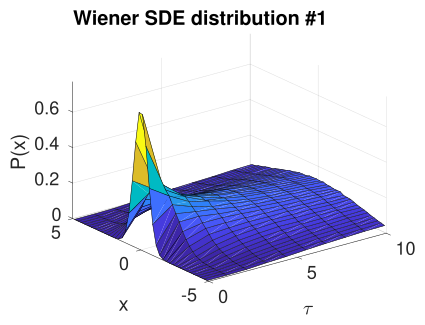
\includegraphics[width=0.75\textwidth]{Wienerprob1} 
\par\end{centering}
\begin{centering}
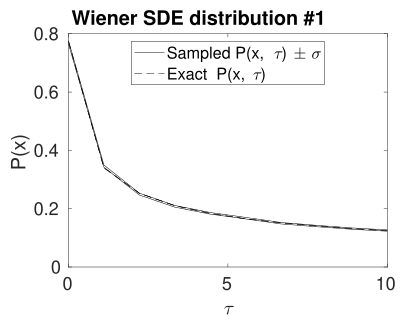
\includegraphics[width=0.75\textwidth]{Wienerprob3} 
\par\end{centering}
\centering{}

\caption{\emph{Top figure: 3D plot of the computed probability density of the
simulated Wiener process as a function of time ($\tau$) and \textquotedblleft position\textquotedblright{}
($x$). Bottom figure: Time evolution of the computed probability
density for $x=0$. The solid lines indicate upper and lower sampling
error bounds, while the dashed line indicates theoretical predictions.}}
\vspace{10pt}
 
\end{figure}

\begin{figure}[H]
\begin{centering}
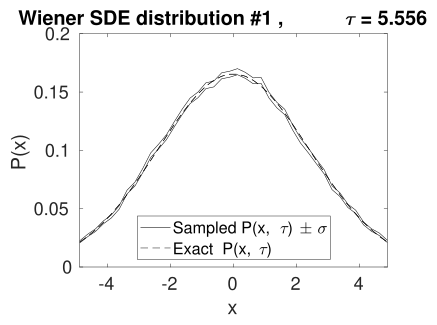
\includegraphics[width=0.75\textwidth]{Wienerprob2} 
\par\end{centering}
\begin{centering}
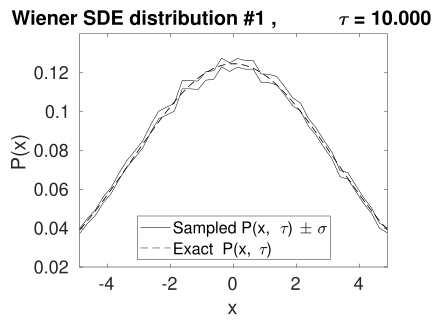
\includegraphics[width=0.75\textwidth]{Wienerprob4} 
\par\end{centering}
\centering{}

\caption{\emph{Top and bottom figure: Computed probability densities of the
simulated Wiener process at $\tau=5.556$ and $\tau=10$, respectively.
In total, 5 of these transverse plots are generated, however, only
2 are presented here.}}
\vspace{10pt}
 
\end{figure}

\pagebreak{}

\section{SPDE examples}

\subsection{Nonlinear Schrodinger equation with Neumann boundary conditions\label{subsec:Nonlinear-Schrodinger-equation}}

This solves a (1+1)-dimensional PSDE with an initial condition of
$a\left(t=0,x\right)=sech\left(x\right)$ and

\begin{eqnarray}
\frac{\partial a}{\partial t} & = & i\cdot\left(a\cdot\left(\left|a\right|^{2}-\frac{1}{2}\right)+\frac{1}{2}\frac{\partial^{2}a}{\partial x^{2}}\right)\,.
\end{eqnarray}
The solution is subject to Neumann boundary conditions with boundary
values at zero

\begin{eqnarray}
\frac{\partial a}{\partial x}\left(t,\pm x_{m}\right) & = & 0\,.
\end{eqnarray}

The equation is a deterministic nonlinear Schrodinger equation, which
applies to nonlinear optics, Bose-Einstein condensates and plasma
physics. The observables are $o_{1}\equiv\left|a\right|^{2}$ and
$o_{2}\equiv\int_{-x_{m}}^{x_{m}}\left|\frac{\partial}{\partial x}a\right|^{2}dx$.

\paragraph{Notes}
\begin{itemize}
\item The boundary conditions are specified with \emph{p.boundaries\{2\},
}which is the x-dimension. 
\item The integration differential $dx$ does not have to be entered, as
this is the default. 
\item Three transverse graphs were specified, but they aren't reproduced
here. 
\item As there is only one field, which is the default, this does not need
to be given. 
\item Since there is no noise, the default integration method was RK4. 
\end{itemize}
\begin{center}
\doublebox{\begin{minipage}[t]{0.9\columnwidth}%
\texttt{function {[}e{]} = SolitonDerivN()}

\texttt{p.dimensions = 2;}

\texttt{p.points = {[}101,101{]};}

\texttt{p.ranges = {[}10,15{]};}

\texttt{p.initial = @(v,p) sech(p.x);}

\texttt{p.observe\{1\} = @(a,p) a.{*}conj(a);}

\texttt{p.observe\{2\} = @(a,p) Int(abs(D1(a,2,p)).\textasciicircum 2,p);}

\texttt{p.olabels = \{'\textbar a\textbar\textasciicircum 2','\textbackslash int
\textbar da/dx\textbar\textasciicircum 2 dx'\};}

\texttt{p.name = 'NLS soliton:spectral method + Neumann';}

\texttt{p.boundaries\{2\} = {[}-1,-1{]};}

\texttt{p.transverse = \{3\};}

\texttt{p.deriv = @(a,\textasciitilde ,p) 1i{*}a.{*}(conj(a).{*}a);}

\texttt{p.linear = @(p) 0.5{*}1i{*}(p.Dx.\textasciicircum 2-1);}

\texttt{e = xspde(p);}

\texttt{end}%
\end{minipage}} 
\par\end{center}

\newpage{}

\begin{figure}[H]
\begin{centering}
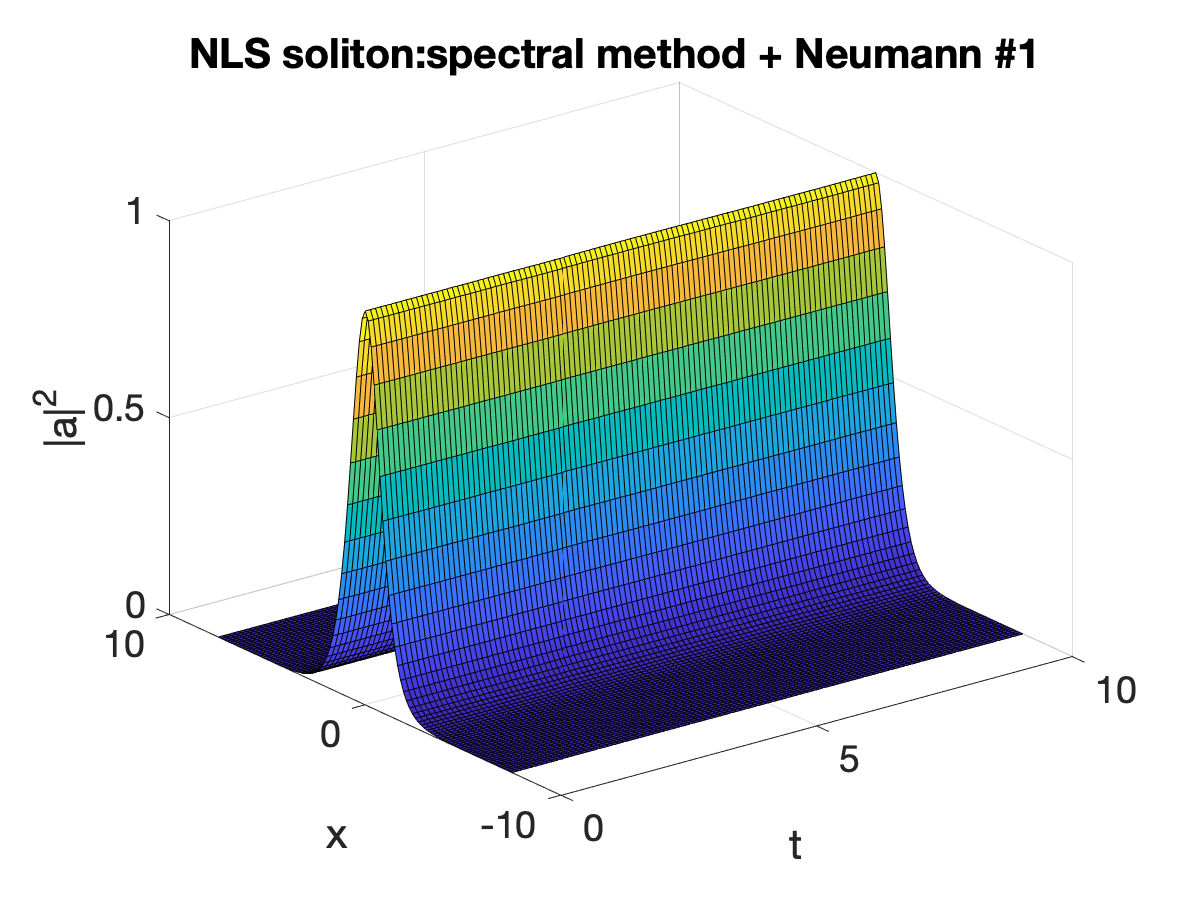
\includegraphics[width=0.75\textwidth]{NLS_Neumann} 
\par\end{centering}
\centering{}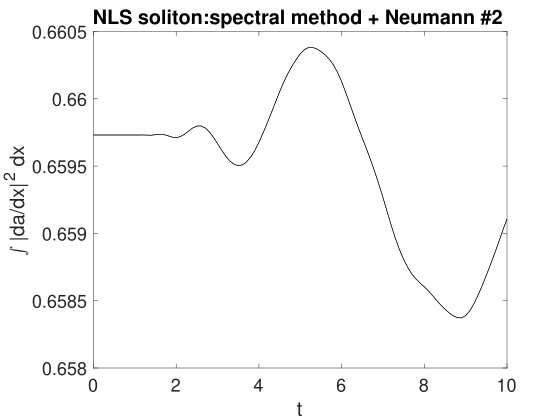
\includegraphics[width=0.75\textwidth]{NLS_Neumann_deriv}

\caption{\emph{Top figure: Evolution of the field modulus squared of an NLS
soliton with Neumann boundaries. }\protect \protect \\
 \emph{Bottom figure: Evolution of the integrated modulus squared
of the gradient for an NLS soliton with Neumann boundaries, showing
how the reflected fields at the boundaries change the result even
though this is not readily visible above.}}
\vspace{10pt}
 
\end{figure}

\pagebreak{}

\subsection{Planar noise growth}

This solves a (1+2)-dimensional PSDE describing the growth of noise
in a planar vector field with a diffraction term giving rise to noise
dispersion. There are $240$ trajectories in the total ensemble. The
equation is:

\begin{eqnarray}
\frac{\partial\mathbf{a}}{\partial t} & = & \frac{i}{2}\left(\frac{\partial^{2}}{\partial x^{2}}+\frac{\partial^{2}}{\partial x^{2}}\right)\mathbf{a}+\mathbf{\eta}\left(t,x\right)\,.
\end{eqnarray}
The initial conditions are that $\mathbf{a}=\left(\mathbf{v}_{x}+i\mathbf{v}_{y}\right)/\sqrt{2}$,
where: 
\begin{equation}
\left\langle v_{i}\left(\mathbf{x}\right)v_{j}\left(\mathbf{x}'\right)\right\rangle =\delta\left(\mathbf{x}-\mathbf{x}'\right)\delta_{ij}
\end{equation}
the noise correlations are that $\mathbf{\eta}=\left(\mathbf{w}_{x}+i\mathbf{w}_{y}\right)/\sqrt{2}$,
where:

\begin{eqnarray}
\left\langle w_{i}\left(\mathbf{r}\right)w_{j}\left(\mathbf{r}'\right)\right\rangle  & = & \delta\left(t-t'\right)\delta_{ij}\left(\mathbf{x}-\mathbf{x}'\right)
\end{eqnarray}

The solution has periodic boundary conditions. The noise correlations
for the second field are specified in momentum space. As there are
no filters specified, the noise terms are delta-correlated in both
momentum ($\mathbf{k}$) and in space ($x$). The exact results for
comparison for the correlations within each field are similar in position
and momentum space: 
\begin{align}
\left\langle \left|a_{i}\left(t,\mathbf{x}\right)\right|^{2}\right\rangle  & =\left(1+t\right)/\Delta A_{x}.\nonumber \\
\left\langle \left|a_{i}\left(t,\mathbf{k}\right)\right|^{2}\right\rangle  & =\left(1+t\right)/\Delta A_{k}.
\end{align}

Here, $\Delta A_{x,k}$ is the area of a lattice cell in space or
momentum space respectively. This is $\Delta A_{x}=1/49$ for the
parameters used here. On integration, the correlation is proportional
to $N_{s}$, the number of points in the spatial lattice, which is
$35^{2}=1225$ for the spatial lattice used here:

\begin{align}
\int\left\langle \left|a_{i}\left(t,\mathbf{x}\right)\right|^{2}\right\rangle d\mathbf{x}=\int\left\langle \left|a_{i}\left(t,\mathbf{k}\right)\right|^{2}\right\rangle d\mathbf{k} & =N_{s}\left(1+t\right).
\end{align}


\paragraph{Notes}
\begin{itemize}
\item All three types of ensemble are used 
\item The much lower sampling error after integration is evident in the
graphs 
\item Spatially resolved graphs show larger sampling errors 
\item The integration method is mid-point, as it is stochastic. 
\item Two k-space noises are specified, but they aren't filtered. 
\item Under these conditions, x-space and k-space noise are identical. 
\end{itemize}
\begin{center}
\doublebox{\begin{minipage}[t]{0.9\columnwidth}%
\texttt{function {[}e{]} = Planar()}

\texttt{p.name = 'Planar noise growth';}

\texttt{p.dimensions = 3;}

\texttt{p.fields = 2;}

\texttt{p.ranges = {[}1,5,5{]};}

\texttt{p.points = 10;}

\texttt{p.noises = {[}2,2{]};}

\texttt{p.ensembles = {[}10,2,12{]};}

\texttt{p.initial = @Initial;}

\texttt{p.deriv = @D\_planar;}

\texttt{p.linear = @Linear;}

\texttt{p.observe\{1\} = @(a,p) Int(a(1,:).{*}conj(a(1,:)),p);}

\texttt{p.observe\{2\} = @(a,p) Int(a(2,:).{*}conj(a(2,:)),p.dk,p);}

\texttt{p.observe\{3\} = @(a,p) real(Ave(a(1,:).{*}conj(a(2,:)),p));}

\texttt{p.observe\{4\} = @(a,p) a(2,:).{*}conj(a(2,:));}

\texttt{p.transforms = \{{[}0,0,0{]},{[}0,1,1{]},{[}0,1,1{]}\};}

\texttt{p.olabels\{1\} = '\textless\textbackslash int\textbar a\_1(x)\textbar\textasciicircum 2
d\textasciicircum 2x\textgreater ';}

\texttt{p.olabels\{2\} = '\textless\textbackslash int\textbar a\_2(k)\textbar\textasciicircum 2
d\textasciicircum 2k\textgreater ';}

\texttt{p.olabels\{3\} = '\textless\textless{} a\_1(k)a\textasciicircum{*}\_2(k)\textgreater\textgreater
';}

\texttt{p.olabels\{4\} = '\textless\textbar a\_2(x)\textbar\textasciicircum 2\textgreater
';}

\texttt{p.compare\{1\} = @(p) (1+p.t){*}p.nspace;}

\texttt{p.compare\{2\} = @(p) (1+p.t){*}p.nspace;}

\texttt{p.compare\{3\} = @(p) 0.0;}

\texttt{e = xspde(p);}

\texttt{end}~\\
 \ 

\texttt{function a0 = Initial(v,\textasciitilde )}

\texttt{a0(1,:) = (v(1,:)+1i{*}v(2,:))/sqrt(2);}

\texttt{a0(2,:) = (v(3,:)+1i{*}v(4,:))/sqrt(2);}

\texttt{end}~\\
 \ 

\texttt{function da = D\_planar(\textasciitilde ,w,\textasciitilde )
\%\%Derivatives}

\texttt{da(1,:) = (w(1,:)+1i{*}w(2,:))/sqrt(2);}

\texttt{da(2,:) = (w(3,:)+1i{*}w(4,:))/sqrt(2);}

\texttt{end }~\\
 \ 

\texttt{function L = Linear(p)}

\texttt{lap = p.Dx.\textasciicircum 2+p.Dy.\textasciicircum 2;}

\texttt{L(1,:) = 1i{*}0.5{*}lap(:);}

\texttt{L(2,:) = 1i{*}0.5{*}lap(:);}

\texttt{end}%
\end{minipage}} 
\par\end{center}

\begin{figure}[H]
\begin{centering}
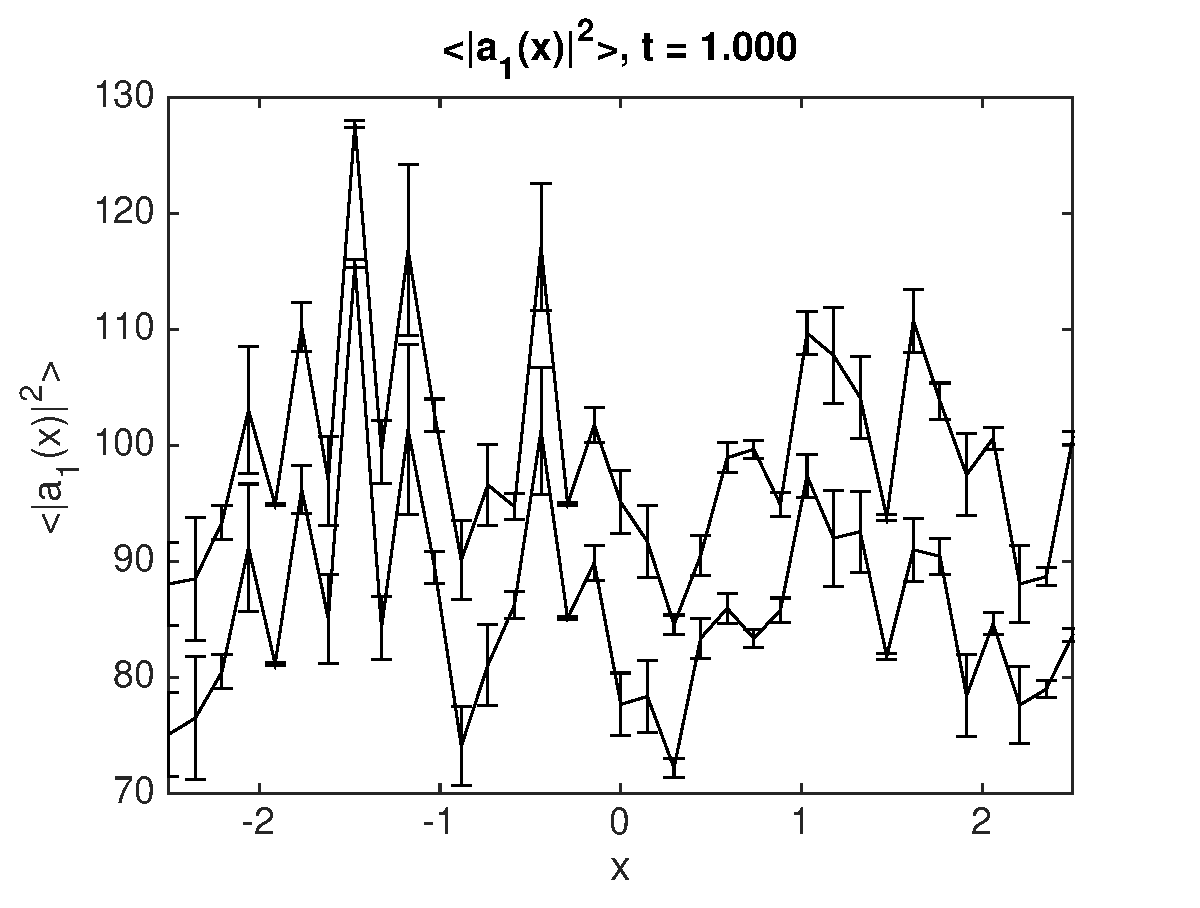
\includegraphics[width=0.75\textwidth]{Planar1} 
\par\end{centering}
\centering{}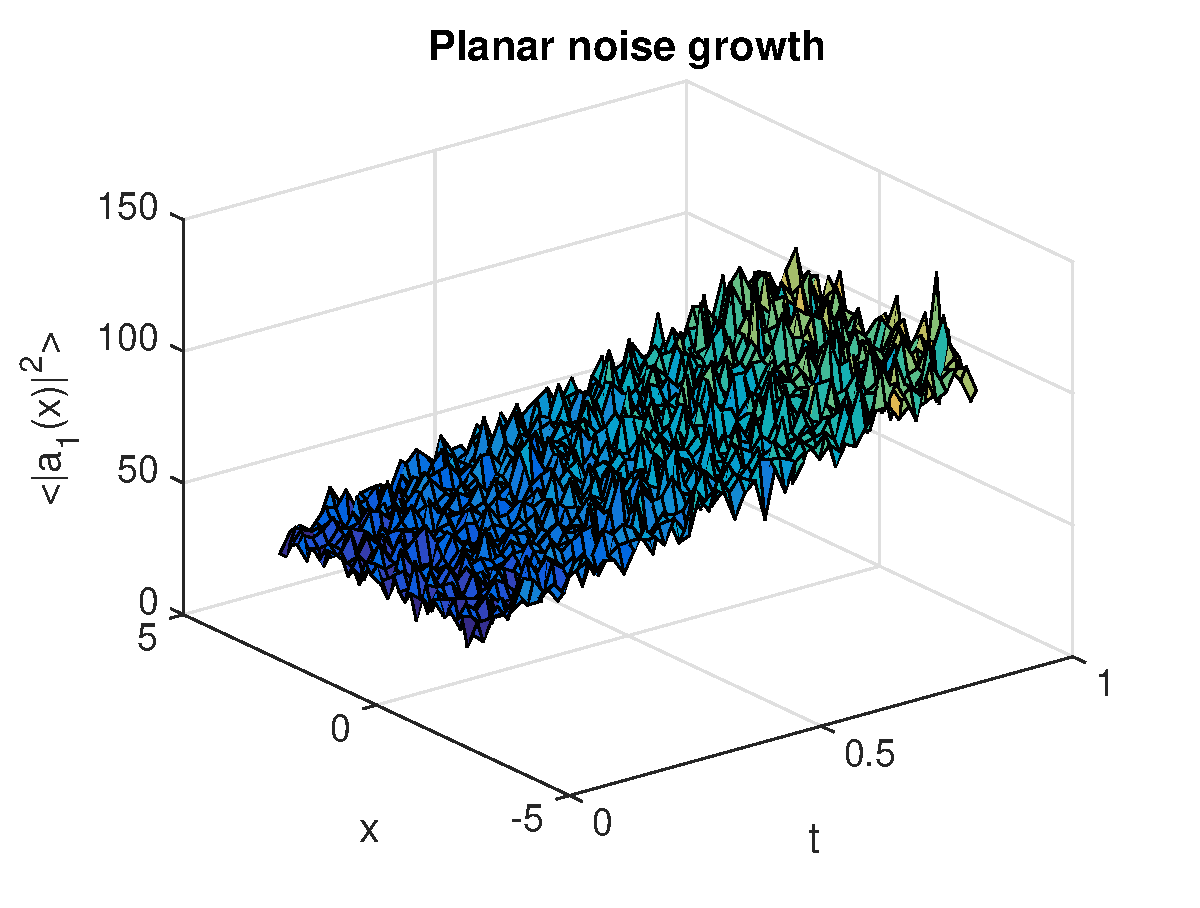
\includegraphics[width=0.75\textwidth]{Planar2}

\caption{\emph{Top and bottom figure: Time evolution of the integrated modulus
square of the first and second field, respectively. The solid lines
indicate upper and lower bounds of the stochastic error, which the
dashed lines indicate theoretical predictions.}}
\vspace{10pt}
 
\end{figure}

\begin{figure}[H]
\begin{centering}
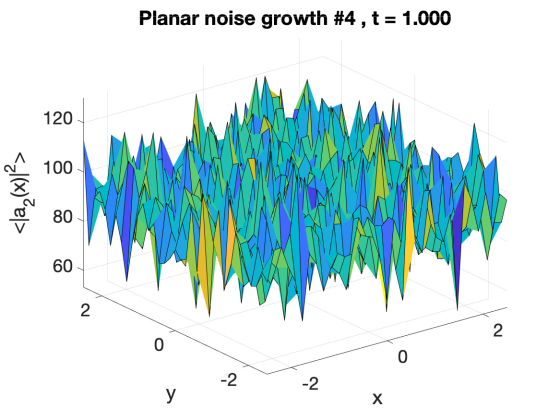
\includegraphics[width=0.75\textwidth]{Planar4image} 
\par\end{centering}
\centering{}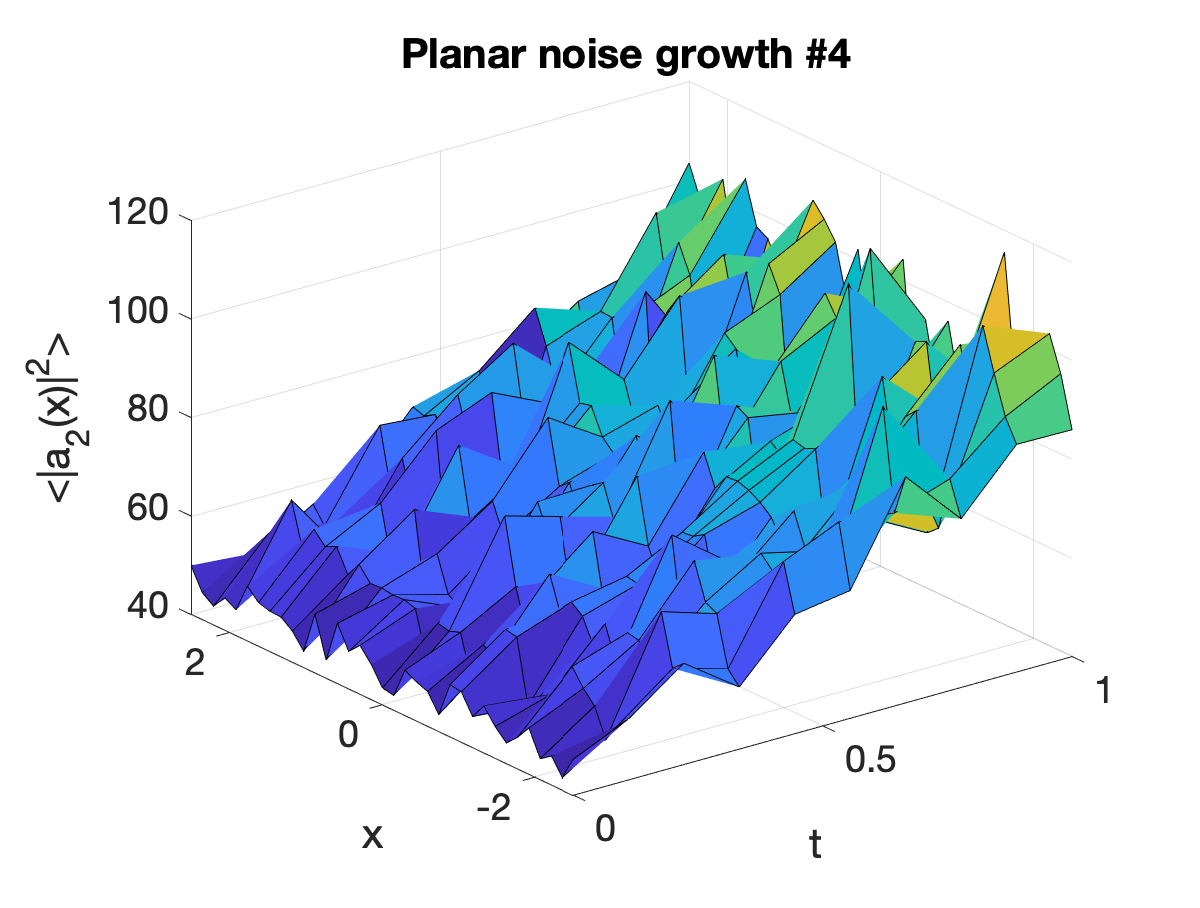
\includegraphics[width=0.75\textwidth]{Planar4}

\caption{\emph{Top figure: 3D plot of the modulus square of $a_{2}$ at $t=1$
as a function of $x$ and $y$. Bottom figure: 3D plot of the modulus
square of $a_{2}$ for $y=0$ as a function of $x$ and $t$.}}
\vspace{10pt}
 
\end{figure}

\pagebreak{}

\subsection{Gross-Pitaevskii equation with vortex formation}

This solves a (1+2)-dimensional PDE called the Gross-Pitaevskii equation.
In addition to the standard GPE terms, it includes the vortex forming
term $\left(\mathbf{x}\times\nabla\right)a$. There is just one ensemble
member, to demonstrate how a single trajectory can be imaged. The
equation is:

\begin{eqnarray}
\frac{\partial a}{\partial t} & = & \left(\frac{1}{2}\nabla^{2}a-\left\Vert \left(\left(V\left(\mathbf{x}\right)+200\left|a\right|^{2}\right)+0.6i\cdot\left(\mathbf{x}\times\nabla\right)\right)a\right\Vert \right)\nonumber \\
V\left(\mathbf{x}\right) & = & 0.35\left(x^{2}+y^{2}\right)\nonumber \\
\left\Vert b\left(\mathbf{x}\right)\right\Vert  & = & \frac{b\left(\mathbf{x}\right)}{\int\left|b\right|^{2}d\mathbf{x}}\,.
\end{eqnarray}

Here,$\left\Vert \cdot\right\Vert $ is the normalized derivative
and $\times$ indicates the two-dimensional cross-product. The system
is initialized as

\begin{eqnarray}
a\left(t=0,\mathbf{x}\right) & = & 0.1\cdot\exp\left(-V\left(\mathbf{x}\right)\right)\,.
\end{eqnarray}


\paragraph{Notes}
\begin{itemize}
\item This is a deterministic partial differential equation case 
\item The $15$ intermediate\emph{ steps }used are necessary to reduce integration
errors 
\item The trap potential is an inline function, and is not a parameter 
\item Normalization is used because otherwise particle number is not conserved 
\item The output includes transverse \emph{images }to show how the vortices
develop 
\item Different \emph{imagetypes} are used to show different 3D features 
\end{itemize}
\begin{center}
\doublebox{\begin{minipage}[t]{0.9\columnwidth}%
\texttt{function {[}e{]} = GPEvortex2D()}

\texttt{p.name = 'GPEvortex2D';}

\texttt{p.dimensions = 3;}

\texttt{p.fields = 1;}

\texttt{p.points = {[}50,40,40{]};}

\texttt{p.ranges = {[}15,16,16{]};}

\texttt{p.steps = 15;}

\texttt{g = 200;}

\texttt{om = 0.6;}

\texttt{L = @(a,p) 1i{*}(p.x.{*}D1(a,3,p)-p.y.{*}D1(a,2,p));}

\texttt{V = @(p) 0.35{*}(p.x.\textasciicircum 2+p.y.\textasciicircum 2);}

\texttt{p.initial = @(v,p) 0.1{*}exp(-V(p));}

\texttt{rho = @(a) g{*}conj(a).{*}a;}

\texttt{p.deriv = @normda;}

\texttt{p.da1 = @(a,w,p) -a.{*}(V(p)+rho(a))+om{*}L(a,p);}

\texttt{p.linear = @(p) 0.5{*}(p.Dx.\textasciicircum 2+p.Dy.\textasciicircum 2);}

\texttt{p.observe\{1\} = @(a,p) a(1,:).{*}conj(a(1,:));}

\texttt{p.observe\{2\} = @(a,p) a(1,:).{*}conj(a(1,:));}

\texttt{p.images = \{2,2\};}

\texttt{p.imagetype = \{1,2\};}

\texttt{p.olabels = \{'\textbar a\textbar\textasciicircum 2','\textbar
a\textbar\textasciicircum 2'\};}

\texttt{e = xspde(p);}

\ 

\texttt{function b = normda(a,w,p)}

\texttt{\% b = NORMDA(a,z,p) is a normalized derivative}

\texttt{\% Takes a derivative and returns a normalized step}

\texttt{b = a+p.da1(a,w,p){*}p.dtr;}

\texttt{norm = sqrt(Int(abs(b).\textasciicircum 2,p.dx,p));}

\texttt{b = (b./norm-a)/p.dtr;}

\texttt{end}

\texttt{end}%
\end{minipage}} 
\par\end{center}

\begin{figure}[H]
\begin{centering}
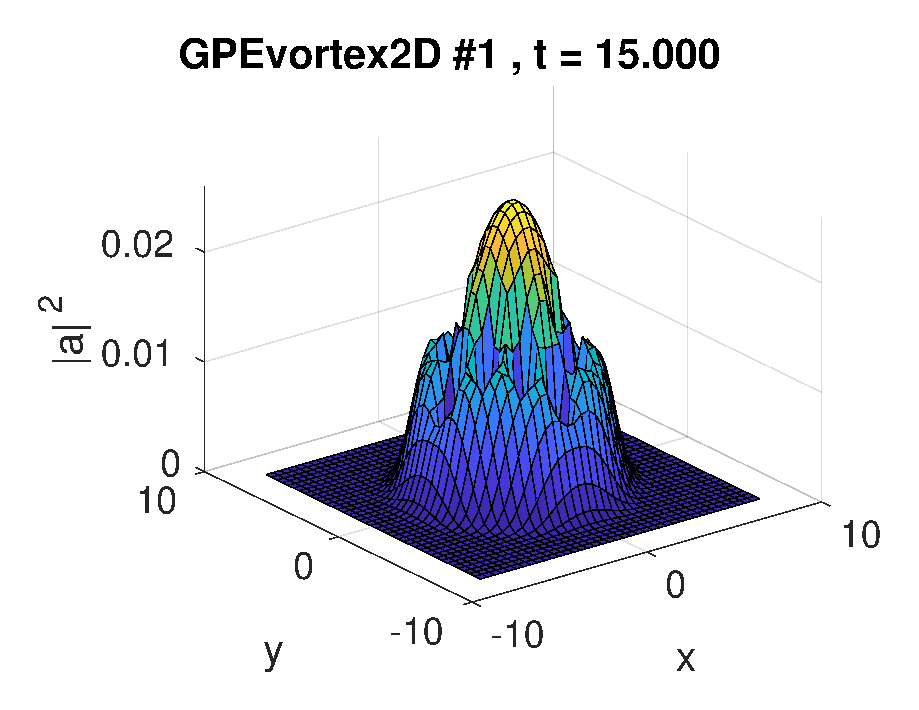
\includegraphics[width=0.75\textwidth]{GPE-vortex-example1} 
\par\end{centering}
\centering{}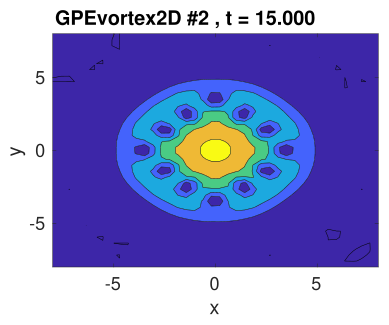
\includegraphics[width=0.75\textwidth]{GPE-vortex-example2}

\caption{\emph{Top and bottom figure: The computed solution for $\left|a\right|^{2}$
at $t=15$ as a function of $x,y$ as a 3D plot (top) and as a color
map (bottom).}}
\vspace{10pt}
 
\end{figure}

\begin{figure}[H]
\begin{centering}
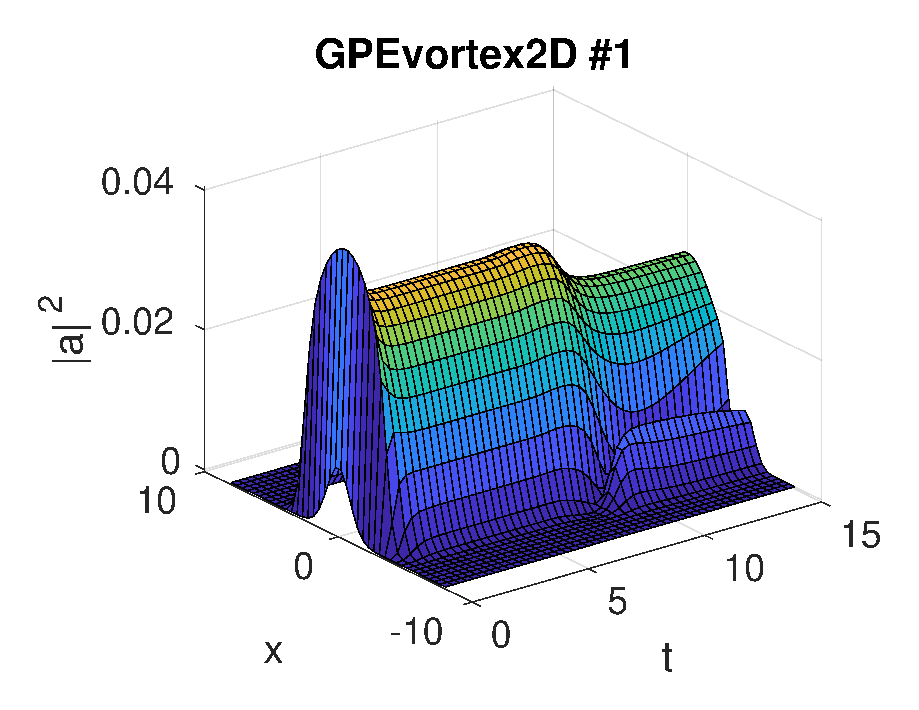
\includegraphics[width=0.75\textwidth]{GPE-vortex-example3} 
\par\end{centering}
\centering{}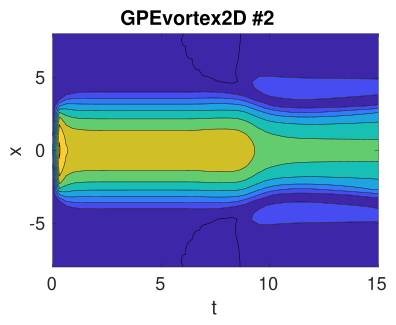
\includegraphics[width=0.75\textwidth]{GPE-vortex-example4}

\caption{\emph{Top and bottom figure: The computed solution for $\left|a\right|^{2}$
for $y=0$ as a function of $x,t$ as a 3D plot (top) and as a color
map (bottom).}}
\vspace{10pt}
 
\end{figure}

\newpage{}

\subsection{Heat equation with finite-difference and propagators \label{subsec:Vector_heat}}

This very simple example solves a (1+1)-dimensional PDE with an initial
condition of $\mathbf{a}\left(t=0,x\right)=\mathbf{f}\left(x\right)$
and

\begin{eqnarray}
\frac{\partial\mathbf{a}}{\partial t} & = & \frac{\partial^{2}\mathbf{a}}{\partial x^{2}}\,.
\end{eqnarray}
The solution is subject to periodic boundary conditions or Dirichlet
and/or Neumann with boundary values at zero, so that $a\left(t,\pm x_{m}\right)=0\,$
or $\partial a/\partial x\left(t,\pm x_{m}\right)=0$. Each component
has different combinations of boundary types. Using spectral methods
the solutions here are exact, up to round-off errors of order $10^{-15}$,
and are also much faster than with finite differences, which is demonstrated
in the example.

In all cases the grid range is from $x=0$ to $x=\pi,$ and the time
duration is from $t=0$ to $t=4$. In the examples, the spectral propagation
error is reduced by more than $10^{10}$ and the time is reduced by
a factor of $20$ compared to the finite-difference methods. The periodic
method has boundaries just outside the grid.

\paragraph*{Dirichlet-Dirichlet}

Here $a_{x}(0)=a_{x}(\pi)=0$, then the exact solution has the form:
\begin{align}
a & =\sum_{n=1}^{\infty}S_{n}\sin\left(nx\right)e^{-n^{2}t}.
\end{align}
Suppose that 
\begin{equation}
a(x,0)=4\sin\left(x\right)+\sin\left(2x\right),
\end{equation}

For this case: 
\begin{equation}
a(x,t)=4\sin\left(x\right)e^{-t}+\sin\left(2x\right)e^{-4t}.
\end{equation}


\paragraph*{Neumann-Neumann}

with $a(0)=a(\pi)=0$, then the exact solution has the form: 
\begin{align}
a & =\sum_{n=0}^{\infty}C_{n}\cos\left(nx\right)e^{-n^{2}t}.
\end{align}
Suppose that 
\begin{equation}
a(x,0)=5+4\cos\left(x\right)+\cos\left(2x\right),
\end{equation}

For this case: 
\begin{equation}
a(x,t)=5+4\cos\left(x\right)e^{-t}+\cos\left(2x\right)e^{-4t}.
\end{equation}


\paragraph*{Dirichlet-Neumann}

Here $a(0)=a_{x}(\pi)=0$, then the exact solution has the form: 
\begin{align}
a & =\sum_{n=1}^{\infty}S_{n}\sin\left((2n-1)x/2\right)e^{-(2n-1)^{2}t/4}.
\end{align}
Suppose that 
\begin{equation}
a(x,0)=4\sin\left(x/2\right)+\sin\left(3x/2\right),
\end{equation}

For this case: 
\begin{equation}
u(x,0)=4\sin\left(x/2\right)e^{-t/4}+\sin\left(3x/2\right)e^{-9t/4}.
\end{equation}


\paragraph*{Neumann-Dirichlet}

Here $a_{x}(0)=a(\pi)=0$, then the general solution has the form:
\begin{align}
a & =\sum_{n=1}^{\infty}C_{n}\cos\left((2n-1)x/2\right)e^{-(2n-1)^{2}t/4}.
\end{align}
Suppose that 
\begin{equation}
a(x,0)=4\cos\left(x/2\right)+\cos\left(3x/2\right).
\end{equation}

For this case: 
\begin{equation}
a(x,t)=4\cos\left(x/2\right)e^{-t/4}+\cos\left(3x/2\right)e^{-9t/4}.
\end{equation}


\paragraph*{Periodic}

Here $a(0)=a(\epsilon\pi)$, where $\epsilon=N/\left(N-1\right)$
accounts for the periodic boundaries being outside the grid range,
then the general solution has the form: 
\begin{align}
a & =\sum_{n=1}^{\infty}S_{n}\sin\left(2nx\right)e^{-4n^{2}t/\epsilon^{2}}\nonumber \\
 & +\sum_{n=0}^{\infty}C_{n}\cos\left(2nx\right)e^{-4n^{2}t/\epsilon^{2}}.
\end{align}
Suppose that 
\begin{equation}
a(x,0)=2+\cos\left(2x/\epsilon\right)+\sin\left(4x/\epsilon\right).
\end{equation}

For this case: 
\begin{equation}
u(x,0)=2+2\cos\left(2x/\epsilon\right)e^{-4t/\epsilon^{2}}+\sin\left(4x/\epsilon\right)e^{-16t/\epsilon^{2}}.
\end{equation}


\paragraph{Notes}
\begin{itemize}
\item This is another deterministic pde case, although noise can be added 
\item Different boundary conditions apply to each component 
\item Sequential integration is used, but the initial condition is just
recycled. 
\item In \emph{p1}, the $40$ intermediate\emph{ steps} are necessary to
reduce finite-difference errors 
\end{itemize}
\doublebox{\begin{minipage}[t]{0.9\columnwidth}%
\texttt{function {[}e{]} = Boundaries()}

\texttt{p.dimensions = 2;}

\texttt{p.points = {[}51,51{]};}

\texttt{p.order = 0;}

\texttt{p.verbose = 1;}

\texttt{p.fields = 5;}

\texttt{p.ranges = {[}4,pi{]};}

\texttt{p.origins = {[}0,0{]};}

\texttt{p.initial = @heat\_in;}

\texttt{p.observe = \{@(a,p) a(1,:),@(a,p) a(2,:),@(a,p) a(3,:)...}

\texttt{@(a,p) a(4,:),@(a,p) a(5,:)\};}

\texttt{p.compare = \{@heat\_1,@heat\_2,@heat\_3,@heat\_4,@heat\_5\};}

\texttt{p.diffplot = \{1,1,1,1,1\};}

\texttt{p.olabels = \{'a, DD','a, NN','a, DN','a, ND','a, PP'\};}

\texttt{p.name = 'Heat test, spectral';}

\texttt{p.boundaries\{2\}= {[}1,1;-1,-1;1,-1;-1,1;0,0{]};}

\texttt{p.linear = @(p) p.Dx.\textasciicircum 2;}

\texttt{p1 = p;}

\texttt{p1.linear = @(p) {[}{]};}

\texttt{p1.deriv = @(a,w,p) D2(a,2,p);}

\texttt{p1.steps = 40;}

\texttt{p1.transfer = @(\textasciitilde ,p,\textasciitilde ,\textasciitilde )
heat\_in(0,p);}

\texttt{p1.name = 'Heat test, finite diffs';}

\texttt{e = xspde(\{p,p1\});}

\texttt{end}

\ 

\texttt{function a = heat\_in(\textasciitilde ,p)}

\texttt{a(1,:) = 4{*}sin(p.x)+sin(2{*}p.x);}

\texttt{a(2,:) = 5+4{*}cos(p.x)+cos(2{*}p.x);}

\texttt{a(3,:) = 4{*}sin(p.x/2)+sin(3{*}p.x/2);}

\texttt{a(4,:) = 4{*}cos(p.x/2)+cos(3{*}p.x/2);}

\texttt{a(5,:) = 2+cos(2{*}p.x/1.02)+sin(4{*}p.x/1.02);}

\texttt{end}

\ 

\texttt{function o = heat\_1(p)}

\texttt{o = 4{*}sin(p.x).{*}exp(-p.t)+sin(2{*}p.x).{*}exp(-4{*}p.t);}

\texttt{end}

\texttt{function o = heat\_2(p)}

\texttt{ o = 5+4{*}cos(p.x).{*}exp(-p.t)+cos(2{*}p.x).{*}exp(-4{*}p.t); }

\texttt{end}

\texttt{function o = heat\_3(p)}

\texttt{ o = 4{*}sin(p.x/2).{*}exp(-p.t/4)+sin(3{*}p.x/2).{*}exp(-9{*}p.t/4); }

\texttt{end}

\texttt{function o = heat\_4(p)}

\texttt{ o = 4{*}cos(p.x/2).{*}exp(-p.t/4)+cos(3{*}p.x/2).{*}exp(-9{*}p.t/4); }

\texttt{end}

\texttt{function o = heat\_5(p)}

\texttt{o = 2+cos(2{*}p.x/1.02).{*}exp(-4{*}p.t/1.02\textasciicircum 2)+...}

\texttt{sin(4{*}p.x/1.02).{*}exp(-16{*}p.t/1.02\textasciicircum 2); }

\texttt{end}%
\end{minipage}}

\newpage{}

\begin{figure}[H]
\centering{}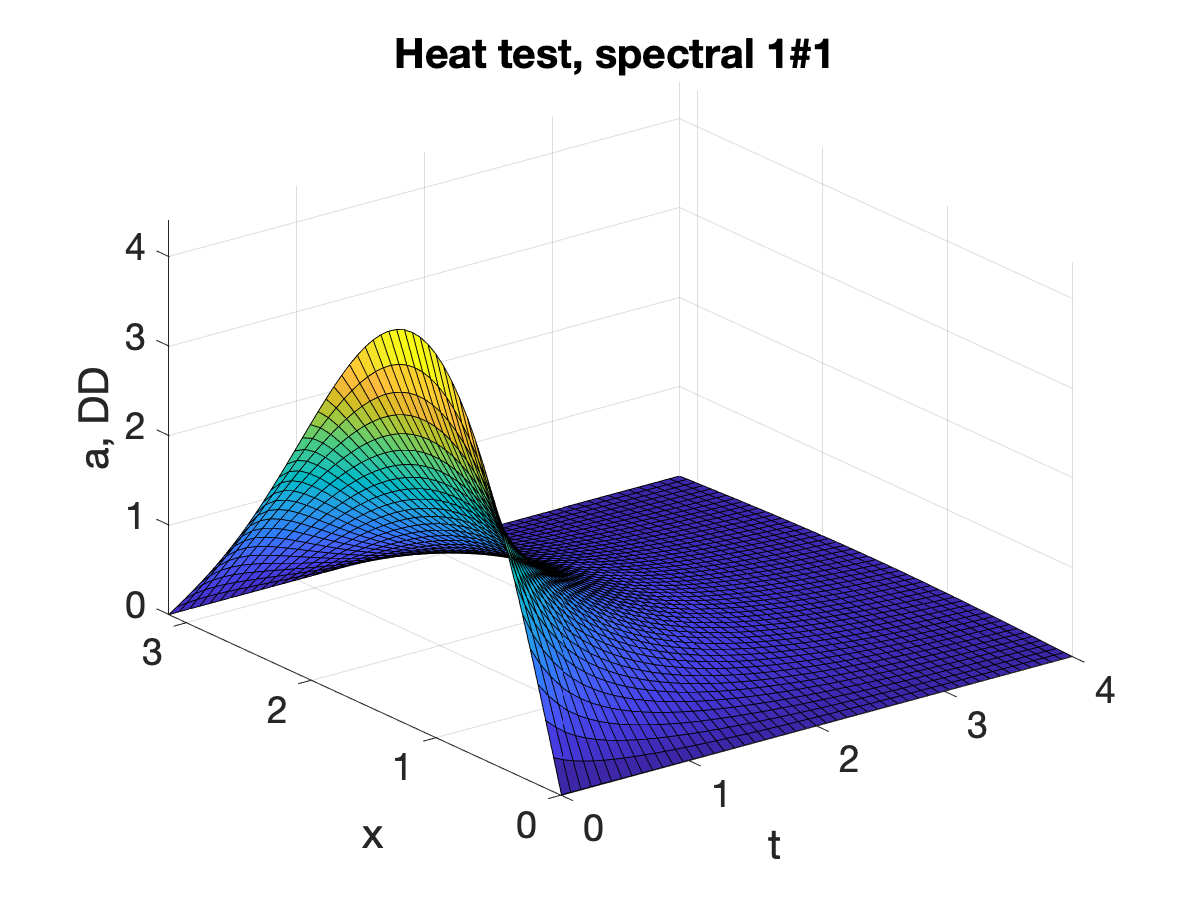
\includegraphics[width=0.75\textwidth]{Boundaries}

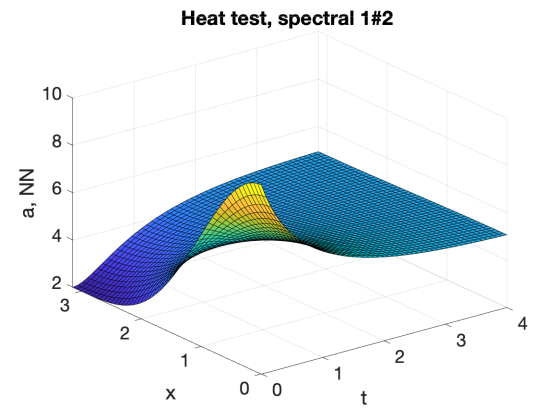
\includegraphics[width=0.75\textwidth]{BoundariesNN}

\caption{\emph{Top figure: Spectral solution for $a$ as a function of time
and position with Dirichlet-Dirichlet boundaries. Bottom figure: Plot
of the solution with Neumann-Neumann boundaries.}}
\vspace{10pt}
 
\end{figure}

\pagebreak{}

\section{Projection examples}

\subsection{SDE with catenoid projection}

This solves an SDE with 3 field variables $\mathbf{a}=\left(a_{1},a_{2},a_{3}\right)^{T}$.
The Stratonovich diffusion equation is 
\begin{eqnarray}
\frac{\partial\mathbf{a}}{\partial t} & = & \mathcal{P}_{\mathbf{a}}^{\parallel}\left[\mathbf{w}\right]\,,
\end{eqnarray}
where $\mathcal{P}_{\mathbf{a}}^{\parallel}\left[\cdot\right]$ indicates
a projected onto the surface of a catenoid manifold defined by 
\begin{eqnarray}
f & =x_{1}^{2}+x_{2}^{2}-\sinh^{2}\left(x_{3}\right)-1 & =0\,.
\end{eqnarray}
The initial condition is given by $\mathbf{a}\left(o\right)=\left(1,0,0\right)^{T}$.
Here $\mathbf{w}=\left(w_{1},w_{2},w_{3}\right)^{T}$ consists of
3 independent noise variables

\paragraph{Notes}
\begin{itemize}
\item This is a projected sde case 
\item The Euclidean distance from the initial point is computed 
\item This is compared with the predicted analytic value $\left\langle R^{2}\right\rangle =2t$. 
\end{itemize}
\begin{center}
\doublebox{\begin{minipage}[t]{0.9\columnwidth}%
\texttt{function {[}e{]} = Catenoid}

\texttt{p.name = '3D Catenoid diffusion';}

\texttt{p.iterproj = 3;}

\texttt{p.X0 = {[}1,0,0{]}';}

\texttt{p.fields = 3;}

\texttt{p.ranges = 5;}

\texttt{p.points = 51;}

\texttt{p.ensembles = {[}400, 10{]};}

\texttt{p.compare\{2\} = @(p) 2{*}p.t;}

\texttt{p.deriv = @(a, w, p) w;}

\texttt{p.initial = @(w, p) p.X0;}

\texttt{p.observe\{2\} = @(a, p) sum((p.X0-a).\textasciicircum 2,1);}

\texttt{p.diffplot\{2\} = 1;}

\texttt{p.function\{1\} = @(o, p) o\{2\}.\textasciicircum 2;}

\texttt{p.olabels = \{'\textbackslash langle R\textasciicircum 2
\textbackslash rangle\textasciicircum 2','\textbackslash langle
R\textasciicircum 2 \textbackslash rangle'\};}

\texttt{p.project = @Catproj;}

\texttt{p.method = @MPnproj;}

\texttt{e = xspde(p);}

\texttt{end}%
\end{minipage}} 
\par\end{center}

\begin{center}
\begin{figure}[H]
\centering{}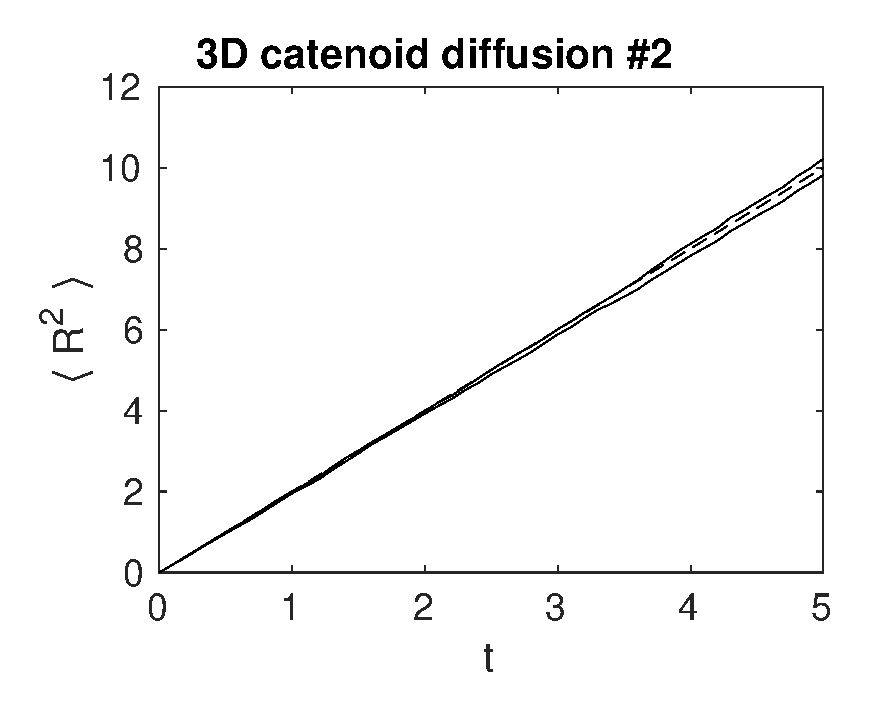
\includegraphics[width=0.75\textwidth]{Catenoid-example1}

\caption{\emph{Computed time evolution of the catenoid squared Euclidean diffusion
distance $\left|\mathbf{x}_{0}-\mathbf{x}\left(t\right)\right|^{2}$,
where $\mathbf{x}_{0}=\left(1,0,0\right)^{T}$, as a function of time.
The solid lines indicate the stochastic error bounds while the dashed
line indicates the theoretical prediction.}}
\vspace{10pt}
 
\end{figure}
\par\end{center}

\begin{center}
\begin{figure}[H]
\centering{}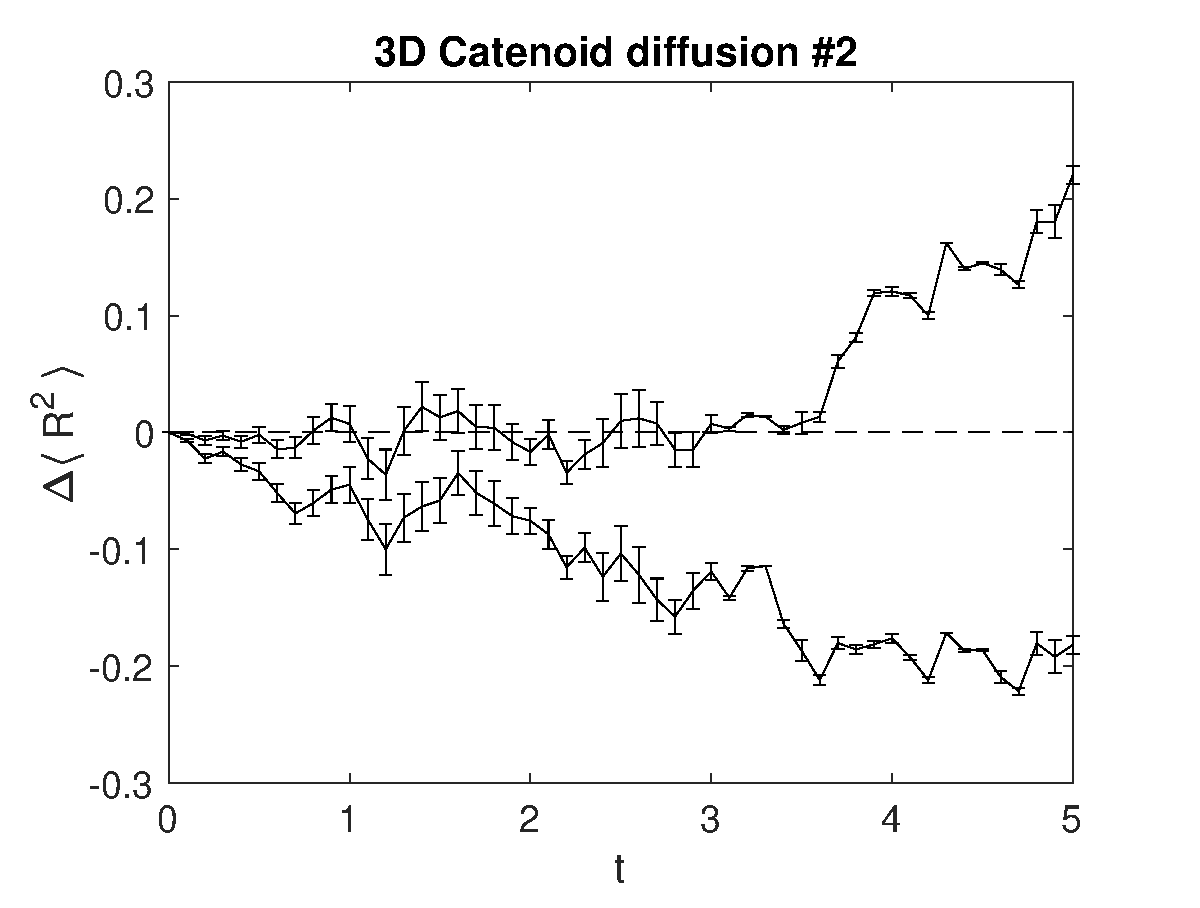
\includegraphics[width=0.75\textwidth]{Catenoid-example2}

\caption{\emph{Differences between the computed time evolution of the catenoid
squared Euclidean distance $\left|\mathbf{x}_{0}-\mathbf{x}\left(t\right)\right|^{2}$
and the exact result. The solid lines indicate the stochastic error
bounds, error-bars are the time-step errors, while the dashed line
indicates the theoretical prediction.}}
\vspace{10pt}
 
\end{figure}
\par\end{center}

\pagebreak{}

\section{Quantum examples}

\subsection{Linear decay, complex SSE}

This solves a standard Lindblad master equation for linear decay with
initial condition $\psi_{j}=\delta_{Nj}$ and $L=\sqrt{\gamma}a$,
$\hat{H}=\hat{a}^{\dagger}\hat{a}$; for $N=6$ , $\gamma=0.25$:
\[
\dot{\rho}=-i[\hat{H},\rho]+2L\rho L^{\dagger}-L^{\dagger}L\rho-\rho L^{\dagger}L
\]

The corresponding Stratonovich SSE is given by:

\[
\frac{d}{dt}\left|\Psi\right\rangle =-i\hat{H}\left|\Psi\right\rangle +\left[\left\langle L^{\dagger}L\right\rangle _{\Psi}-L_{m}^{\dagger}L_{m}+\left(\sqrt{2}\xi+2\left\langle L^{\dagger}\right\rangle _{\Psi}\right)\left(L-\left\langle L_{m}\right\rangle \right)\right]\left|\Psi\right\rangle 
\]

where: 
\[
\left\langle \xi_{j}\left(t\right)\xi_{j}^{*}\left(t'\right)\right\rangle =\delta_{kj}\delta\left(t-t'\right).
\]
The function uses the MPS algorithm together with the SSE derivative,
and compares it with the solution that 
\[
\left\langle \hat{n}\right\rangle =\left\langle \hat{n}\left(0\right)\right\rangle e^{-2t\kappa}.
\]

Both the sparse and functional methods give identical results.

\paragraph{Sparse operator method}
\begin{center}
\doublebox{\begin{minipage}[t]{0.9\columnwidth}%
\texttt{function {[}e{]} = SSElinsp}

\texttt{\%Uses SSE for linear decay with sparse methods}

\texttt{p.name = 'SSE-sparse decay, N=6 initially';}

\texttt{p.N = 6;}

\texttt{p.nmax = p.N+1;}

\texttt{p.ranges = 2;}

\texttt{p.a = mkbose(p);}

\texttt{p.quantum = 1;}

\texttt{p.sparse = 1;}

\texttt{p.ensembles = {[}100,1, 10{]};}

\texttt{p.gamma\{1\} = @(p)0.25;}

\texttt{p.compare\{1\} = @(p) p.N{*}exp(-2{*}p.t{*}p.gamma\{1\});}

\texttt{p.L\{1\} = p.a;}

\texttt{p.H = @(p)p.a\{1\}'{*}p.a\{1\};}

\texttt{p.diffplot = 1;}

\texttt{p.initial = @(w,p) {[}0,0,0,0,0,0,1{]}';}

\texttt{p.expect\{1\} = @(p) p.a\{1\}'{*}p.a\{1\};}

\texttt{p.olabels = \{'\textbackslash langle N \textbackslash rangle','\textbackslash langle
N \textbackslash rangle'\};}

\texttt{e = xsde(p);}

\texttt{end}%
\end{minipage}} 
\par\end{center}

\begin{flushleft}
With the sparse method, the function 'mkbose' is used to create the
operator matrix cell array '\emph{p.a}', before it is used. These
are only generated as needed. For large numbers of modes they can
use a large amount of storage, even though they are sparse matrices.
The use of p.L\{1\} indicates the first decay type is a linear loss,
but there could be other dissipative processes as well. 
\par\end{flushleft}

The use of \emph{p.quantum=1 }shows that it is a stochastic wavefunction
problem, while \emph{p.sparse=1 }indicates the use of sparse matrices.

\paragraph{Function operator method}
\begin{flushleft}
\doublebox{\begin{minipage}[t]{0.9\columnwidth}%
\texttt{function {[}e{]} = SSElin}

\texttt{\%Uses an SSE to solve for a linear decay}

\texttt{p.name = 'SSE linear decay, N=6 initial photons';}

\texttt{p.N = 6;}

\texttt{p.nmax = p.N+1;}

\texttt{p.ranges = 2;}

\texttt{p.quantum = 1;}

\texttt{p.ensembles = {[}100, 10{]};}

\texttt{p.gamma\{1\} = @(p) 0.25;}

\texttt{p.H = @(psi,p) n(1,psi);}

\texttt{p.compare = @(p) p.N{*}exp(-2{*}p.t{*}p.gamma\{1\});}

\texttt{p.L\{1\} = @a;}

\texttt{p.diffplot = 1;}

\texttt{p.initial = @(w,psi) {[}0,0,0,0,0,0,1{]}';}

\texttt{p.expect = @(psi,p) n(1,psi);}

\texttt{p.olabels = \{'\textbackslash langle N \textbackslash rangle'\};}

\texttt{e = xsde(p);}

\texttt{end}%
\end{minipage}} 
\par\end{flushleft}

\begin{flushleft}
With the function method, the function '\emph{mkbose}' is not required.
Instead, the effect of the operators is obtained through a function
call to the handle '\emph{@a}' . For large numbers of modes this method
uses a reduced amount of memory as there is no stored matrix involved
in this case. 
\par\end{flushleft}

One cannot simply write \emph{p.H=@n }here, because the Hamiltonian
is a function of the wavefunction $psi$ and the parameters \emph{p,
}while the number operator is a function of the mode number and the
wavefunction. For Linblad operators, these arguments are inserted
automatically.

The flag \emph{p.diffplot =1 }is used by the graphics code to create
a plot of the difference between the comparison solution and the simulation.

Note that one can determine the relative size of the sampling errors
and step-size errors from the difference plot, although these are
also printed out.

\begin{figure}[H]
\begin{centering}
\includegraphics[width=0.6\textwidth]{SSElin1}\\
 \includegraphics[width=0.6\textwidth]{SSElin2} 
\par\end{centering}
\caption{\emph{Example: Linear decay, including a comparison with the exact
result, below. The graph shows the sampling error-bars as two parallel
lines. The discretization error-bars are less than the minimum, and
are not shown.}}
\vspace{10pt}
 
\end{figure}

\pagebreak{}

\subsection{Time-dependent decay, real SSE}

This solves a Lindblad master equation for linear time-dependent decay
with two modes. and real noises, corresponding to homodyne detection.
The initial condition is $\psi_{j}=\delta_{Nj}$ and $L_{1}=a$, for
$\bm{N}=[3,6]$ .

The decay rates are: 
\begin{align*}
\gamma_{1} & =[0.5,1]*t
\end{align*}
As above, the sparse and functional methods give identical results,
but the sparse method is faster. For comparison purposes, the following
results are expected: 
\[
\bm{N}=[3e^{-t^{2}/2},6e^{-t^{2}}]
\]


\paragraph{Sparse operator method}
\begin{center}
\doublebox{\begin{minipage}[t]{0.9\columnwidth}%
\texttt{function e = SSElin2spr}

\texttt{\%Uses a sparse SSE to solve for a linear two-mode decay}

\texttt{p.name = 'SSE sparse real, N = 3,6';}

\texttt{p.N = 3;}

\texttt{p.Om = 1;}

\texttt{p.noises = 4;}

\texttt{p.ranges = 2;}

\texttt{p.nmax = {[}p.N+1,2{*}p.N+1{]};}

\texttt{p.a = mkbose(p);}

\texttt{p.quantum = 1;}

\texttt{p.sparse = 1;}

\texttt{p.ensembles = {[}100,1,10{]};}

\texttt{p.alpha\{1\} = {[}1,1{]};}

\texttt{p.gamma\{1\} = @(p) {[}0.5,1{]}{*}p.t;}

\texttt{p.L\{1\} = p.a;}

\texttt{p.H = @(p) p.Om{*}(p.a\{1\}'{*}p.a\{1\}+p.a\{2\}'{*}p.a\{2\});}

\texttt{p.initial = @(\textasciitilde ,p) kron({[}0,0,0,1{]},{[}0,0,0,0,0,0,1{]})';}

\texttt{p.expect\{1\} = @(p) p.a\{1\}'{*}p.a\{1\};}

\texttt{p.expect\{2\} = @(p) p.a\{2\}'{*}p.a\{2\};}

\texttt{p.compare\{1\} = @(p) p.N{*}exp(-p.t.\textasciicircum 2/2);}

\texttt{p.compare\{2\} = @(p) 2{*}p.N{*}exp(-p.t.\textasciicircum 2);}

\texttt{p.diffplot = \{1,1\};}

\texttt{p.olabels = \{'\textless{} n\_1 \textgreater ','\textless{}
n\_2 \textgreater '\};}

\texttt{e = xsde(p);}

\texttt{end}%
\end{minipage}} 
\par\end{center}

The use of \emph{p.quantum=1 }shows that it is a stochastic wavefunction
problem, while \emph{p.sparse=1 }indicates sparse matrices, and \emph{p.alpha
= \{{[}1,1{]}\} }specifies that all channels have real noises.

\paragraph{Function operator method}
\begin{flushleft}
\doublebox{\begin{minipage}[t]{0.9\columnwidth}%
\texttt{function e = SSElin2r}

\texttt{\%Uses a non-sparse SSE to solve for a linear two-mode decay}

\texttt{p.name = 'SSE, N = 3,6';}

\texttt{p.N = 3;}

\texttt{p.Om = 1;}

\texttt{p.ranges = 2;}

\texttt{p.nmax = {[}p.N+1,2{*}p.N+1{]};}

\texttt{p.quantum = 1;}

\texttt{p.ensembles = {[}100, 10{]};}

\texttt{p.gamma\{1\} = @(p){[}0.5,1{]}{*}p.t;}

\texttt{p.alpha\{1\} = {[}1,1{]};}

\texttt{p.L\{1\} = @a;}

\texttt{p.H = @(psi,p) p.Om{*}(n(1,psi)+n(2,psi));}

\texttt{p.initial = @(\textasciitilde ,p) kron({[}0,0,0,1{]}',{[}0,0,0,0,0,0,1{]});}

\texttt{p.expect\{1\} = @(psi,p) n(1,psi);}

\texttt{p.expect\{2\} = @(psi,p) n(2,psi);}

\texttt{p.compare\{1\} = @(p) p.N{*}exp(-p.t.\textasciicircum 2/2);}

\texttt{p.compare\{2\} = @(p) 2{*}p.N{*}exp(-p.t.\textasciicircum 2);}

\texttt{p.olabels = \{'n\_1','n\_2'\};}

\texttt{e = xsde(p);}

\texttt{end}%
\end{minipage}} 
\par\end{flushleft}

\begin{flushleft}
With the function method, the function '\emph{mkbose}' is not required.
Instead, the effect of the operators is obtained through a function
call to the handles '\emph{@a}' and '\emph{@a}2' . For large numbers
of modes this method uses a reduced amount of memory as there is no
stored matrix involved in this case. 
\par\end{flushleft}

\begin{figure}[H]
\begin{centering}
\includegraphics[width=0.75\textwidth]{SSElin2r_1}\\
 \includegraphics[width=0.75\textwidth]{SSElin2r_2} 
\par\end{centering}
\caption{\emph{Example: SSE linear decay, with a time-dependent decay rate..
Top graph has $N=3$ , lower graph has $N=6.$}}
\vspace{10pt}
 
\end{figure}

\pagebreak{}

\subsection{Nonlinear decay, real SSE}

This solves a Lindblad master equation for nonlinear decay with two
modes and two decay channels. The initial condition is $\psi_{j}=\delta_{Nj}$
and $L_{1}=a$, $L_{2}=a^{2}$, for $N=[3,6]$ .

The decay rates are: 
\begin{align*}
\gamma_{1} & =[0.01,0.01]\\
\gamma_{2} & =[.5,.25],
\end{align*}
The function uses the MPS algorithm with the SSE derivative, and has
real noise terms. The sparse and functional methods give identical
results, but the sparse method is faster.

\paragraph{Sparse operator method}
\begin{center}
\doublebox{\begin{minipage}[t]{0.9\columnwidth}%
\texttt{function e = SSEnonlin2spr}

\texttt{\%Uses a real sparse SSE to solve for nonlinear two-mode decay}

\texttt{p.name = 'Real sparse SSE, M=2, N=3,6';}

\texttt{p.nmax = {[}4,7{]};}

\texttt{p.steps = 8;}

\texttt{p.a = mkbose(p);}

\texttt{p.a2 = mkbose(1:2,2,p);}

\texttt{p.ensembles = {[}10,10,10{]};}

\texttt{p.quantum = 1;}

\texttt{p.sparse = 1;}

\texttt{p.gamma = \{@(p){[}0.01,0.01{]},@(p){[}.5,.25{]}\};}

\texttt{p.alpha = \{{[}1,1{]},{[}1,1{]}\};}

\texttt{p.L = \{p.a,p.a2\};}

\texttt{p.initial = @(\textasciitilde ,p) kron({[}0,0,0,1{]},{[}0,0,0,0,0,0,1{]})';}

\texttt{p.expect\{1\} = @(p) p.a\{1\}'{*}p.a\{1\};}

\texttt{p.expect\{2\} = @(p) p.a\{2\}'{*}p.a\{2\};}

\texttt{p.olabels = \{'n\_1','n\_2'\};}

\texttt{e = xsde(p);}

\texttt{end}%
\end{minipage}} 
\par\end{center}

\begin{flushleft}
With the sparse method, the function 'mkbose' is used twice to create
the operator matrix cell array '\emph{p.a}', and '\emph{p.a}2' before
they are used. 
\par\end{flushleft}

The use of \emph{p.quantum=1 }shows that it is a stochastic wavefunction
problem, while \emph{p.sparse=1 }indicates sparse matrices, and \emph{p.alpha
= \{{[}1,1{]},{[}1,1{]}\} }specifies that all channels have real noises.

\paragraph{Function operator method}
\begin{flushleft}
\doublebox{\begin{minipage}[t]{0.9\columnwidth}%
\texttt{function e = SSEnonlin2r}

\texttt{\%Uses an SSE to solve for a linear two-mode decay}

\texttt{p.name = 'Real nonlinear SSE, 2-modes, N = 3,6';}

\texttt{p.nmax = {[}4,7{]};}

\texttt{p.steps = 8;}

\texttt{p.ensembles = {[}10,10,10{]};}

\texttt{p.quantum = 1;}

\texttt{p.gamma = \{@(p){[}0.01,0.01{]},@(p) {[}.5,.25{]}\};}

\texttt{p.L = \{@a,@a2\};}

\texttt{p.alpha = \{{[}1,1{]},{[}1,1{]}\};}

\texttt{p.initial = @(\textasciitilde ,p) kron({[}0,0,0,1{]}',{[}0,0,0,0,0,0,1{]});}

\texttt{p.expect\{1\} = @(psi,p) n(1,psi);}

\texttt{p.expect\{2\} = @(psi,p) n(2,psi);}

\texttt{p.olabels = \{'n\_1','n\_2'\};}

\texttt{e = xsde(p);}

\texttt{end}%
\end{minipage}} 
\par\end{flushleft}

\begin{flushleft}
With the function method, the function '\emph{mkbose}' is not required.
Instead, the effect of the operators is obtained through a function
call to the handles '\emph{@a}' and '\emph{@a}2' . For large numbers
of modes this method uses a reduced amount of memory as there is no
stored matrix involved in this case. 
\par\end{flushleft}

\begin{figure}[H]
\begin{centering}
\includegraphics[width=0.75\textwidth]{SSEnonlin1}\\
 \includegraphics[width=0.75\textwidth]{SSEnonlin2} 
\par\end{centering}
\caption{\emph{Example: SSE nonlinear decay, with a small linear decay., real
noise and either odd or even number starting points.Top graph has
$N=3$ , lower graph has $N=6.$}}
\vspace{10pt}
 
\end{figure}


\section*{Acknowledgements}

We would like to thank the many users and researchers whose feedback
was invaluable, including Rodney Polkinghorne, Simon Kiesewetter,
Bogdan Opanchuk, King Ng, Alex Dellios, Run Yan Teh, Manushan Thenabadu,
Margaret Reid, Jesse van Rhijn and Thomas Rodriguez. This work was
funded through the Australian Research Council Discovery Project scheme
under Grants DP180102470 and DP190101480. The authors also wish to
thank NTT Research and the Templeton Foundation for their financial
and technical support.

\bibliographystyle{SciPost_bibstyle}
\bibliography{xSPDE4}

\end{document}
